\documentclass[11pt]{article}
\usepackage[web]{../problem-collection}
\begin{document}

\begin{titlepage}
    \centering
    \vspace{10cm}
    {\sffamily\Huge \mbox{180 EESTI FÜÜSIKAOLÜMPIAADI}\\ PÕHIKOOLI ÜLESANNET AASTATEST\\ 2006 -- 2020?\par}
    \vspace{1cm}
    {\Large koos vihjete ja lahendustega\par}
    \vfill
    {\Large Koostas Raimond Pääru}

    \vfill

    % Bottom of the page
    {\large 2019}
\end{titlepage}

\raggedbottom % Because of twosided
\mbox{}\vfill

\textcopyright~Autoriõigused: ...

\vfill

Toimetas ja kontrollis Roland Erich Uriko

Kirjastanud Tallinna Tehnikaülikooli eelõppeosakond
\vspace{0.5\baselineskip}
\newpage

\tableofcontents
\newpage

{\setlength{\parindent}{24pt}
\section{Sissejuhatus}

Siia on koondatud 180 põhikooli ülesannet Eesti füüsikaolümpiaadi piirkonnavoorudest ja lõppvoorudest.
Igale ülesandele on juurde kirjutatud lühike vihje.
Juhul kui õpilane jääb ülesannet lahendades toppama, on tal võimalik vihjet lugeda ning teisele katsele minna.

Ülesanded on jaotatud teemade kaupa ning teemasiseselt raskuse järgi. Raskustaset tähistatakse kuni viie tärniga.
Ülesannete lihtsamaks otsimiseks on ülesannete numbrite ette pandud Ü vihjete ette V ja lahenduste ette L.
Näiteks ülesande 69 teksti number on kujul Ü69.
Iga ülesande juures on kirjas ka selle autor (kui see on teada) ning olümpiaadi vooru lühinimetus, lisaks lühendid P 1, G 1 jne, kus tähed tähistavad põhikooli- ja gümnaasiumiastet.
Näiteks P 9 viitab põhikooliastme 9. ülesandele.
\newpage
\setlength{\parindent}{0pt}

        \section{Ülesanded}
        \ToggleStatement
        \subsection{\protect\StrSubstitute{Elektriõpetus}{-}{ }}

\graphicspath{{Kogumik_new/}}

% Ü1
\ylDisplay{Lüliti} % Ülesande nimi
{Tundmatu autor} % Autor
{piirkonnavoor} % Voor
{2012} % Aasta
{P 3} % Ülesande nr.
{1} % Raskustase
{
% Teema: Elektriõpetus
\ifStatement
Juku tahab ehitada seadet, mis elektrimootori jõul kardinaid akna ette või eest ära tõmbaks. Selleks võttis ta elektrimootori, lüliti ja suure patarei. Kasutatud lüliti võib olla kolmes asendis ja sellel on 6 klemmi. Lambi ja patareiga katsetades sai Juku teada, et erinevates asendites (A, B või C) ühendab lüliti klemme kokku joonisel kujutatud viisil. Mootor muudab suunda, kui temaga ühendatud patarei klemmid ära vahetada. Kuidas peaks ühendama lüliti, patarei ja mootori, et lüliti erinevate asendite korral pöörleks mootor ühtepidi, teistpidi või oleks  paigal? Joonistage kaks elektriskeemi, kus on lülitit erinevalt kasutatud.
\begin{center}
	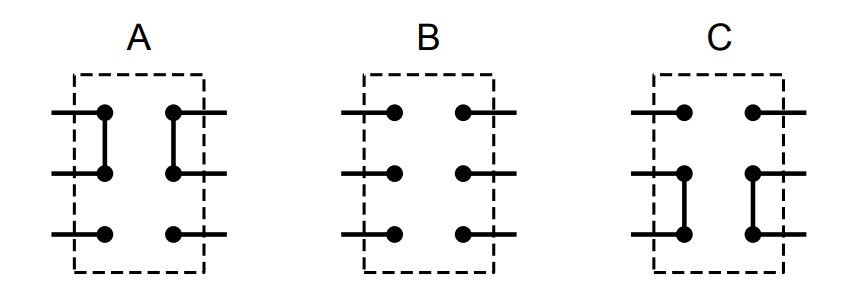
\includegraphics[width=0.5\linewidth]{2012-v2p-03-yl.png}
\end{center}
\fi
}

% Ü2
\ylDisplay{Takistid} % Ülesande nimi
{Tundmatu autor} % Autor
{piirkonnavoor} % Voor
{2006} % Aasta
{P 6} % Ülesande nr.
{2} % Raskustase
{
% Teema: Elektriõpetus
\ifStatement
On kaks takistit. Kui ühendada alalispinge-allikaga eraldi esimene takisti, siis sellel eraldub võimsus $P_1 = 10$ $W$. Kui ühendada eraldi teine takisti, siis takistil eraldub võimsus $P_2 = 15$ $W$. Kui suur summaarne võimsus eraldub pingeallikaga ühendatud takistitel, kui nad ühendada omavahel: a) rööbiti; b) jadamisi?
\fi
}

% Ü3
\ylDisplay{Takistite ühendused} % Ülesande nimi
{Tundmatu autor} % Autor
{piirkonnavoor} % Voor
{2008} % Aasta
{P 5} % Ülesande nr.
{2} % Raskustase
{
% Teema: Elektriõpetus
\ifStatement
Antud on kolm takistit väärtustega $R_1 = 1$ $\Omega$, $R_2 = 2$ $\Omega$ ja $R_3 = 3$ $\Omega$. Milliseid erinevaid kogutakistuse väärtusi võib saada neid omavahel kahe- või kolmekaupa kõikvõimalikel viisidel ühendades?
\fi
}

% Ü4
\ylDisplay{Pirnid} % Ülesande nimi
{Tundmatu autor} % Autor
{piirkonnavoor} % Voor
{2009} % Aasta
{P 7} % Ülesande nr.
{2} % Raskustase
{
% Teema: Elektriõpetus
\ifStatement
Urmol oli neli pirni, neist kolm uhesugused. Kui Urmo ühendas pirnid joonisel kujutatud viisil tundmatu pingeallikaga, põlesid nad kõik sama võimsusega. Pirnil 1 oli kirjas ”$10$ $W$”. Mis oli kirjas pirnidel $2$, kui on teada, et kõik pirnid on sama nimipingega? Lambi takistuse sõltuvusega temperatuurist mitte arvestada.
\begin{center}
	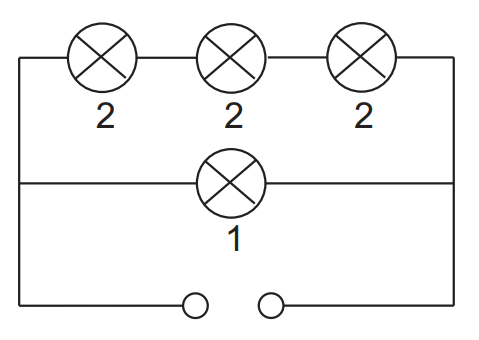
\includegraphics[width=0.5\linewidth]{2009-v2p-07-yl.png}
\end{center}
\fi
}

% Ü5
\ylDisplay{Traat} % Ülesande nimi
{Tundmatu autor} % Autor
{piirkonnavoor} % Voor
{2010} % Aasta
{P 5} % Ülesande nr.
{2} % Raskustase
{
% Teema: Elektriõpetus
\ifStatement
Mikk tahtis teada, kui pikk on pooliks keritud üliõhukese isolatsioonikihiga kaetud raudtraat. Kuna Mikk oli lõpetamas põhikooli, otsustas ta traadi pikkuse määramiseks kasutada oma füüsikateadmisi. Ta võttis traatpooli kooli kaasa ja pärast tunde tegi füüsikakabinetis vajalikud mõõtmised. Selgus, et traadi mass $m = 400$ $g$. Pinge $U = 4$ $V$ rakendamisel traadi otstele tekkis traadis vool tugevusega $I = 0,2$ $A$. Ta leidis füüsikaliste suuruste tabelitest, et raua tihedus $d = 7850$ $kg/m^3$ ja raua eritakistus $\rho = 0,098 \cdot 10 - 6 \Omega \cdot m$. Arvutage traadi pikkus.
\fi
}

% Ü6
\ylDisplay{Vaskrõngas} % Ülesande nimi
{Tundmatu autor} % Autor
{piirkonnavoor} % Voor
{2011} % Aasta
{P 5} % Ülesande nr.
{2} % Raskustase
{
% Teema: Elektriõpetus
\ifStatement
Vasktraadist rõngas ühendatakse vooluringi punktide $A$ ja $B$ kaudu. Rõnga umbermõõt  $l = 60$ $cm$, traadi läbimõõt $d = 0,1$ $mm$ ja eritakistus $\rho = 0,017$ $\Omega \frac{mm^2}{m}$. Kui suur on punktide $A$ ja $B$ vaheline pinge, kui rõnga lühema kaare pikkus on $1/3$ rõnga ümbermõõdust ja voolutugevus rõngast vooluallikaga ühendavates juhtmetes $I = 0,2$ $A$?
\fi
}


% Ü7
\ylDisplay{Küttekeha} % Ülesande nimi
{Tundmatu autor} % Autor
{lõppvoor} % Voor
{2012} % Aasta
{P 6} % Ülesande nr.
{2} % Raskustase
{
% Teema: Elektriõpetus
\ifStatement
Juku tahab endale ehitada võimalikult võimsat veekeetjat. Selleks on tal küttekeha alusplaat, millele saab ühendada takisteid nagu näidatud joonisel, ja $4$ takistit, mille takistused on $30$ $\Omega$, $20$ $\Omega$, $15$ $\Omega$ ja $10$ $\Omega$. Kuidas peaks ta takistid plaadil olevatesse pesadesse paigutama, et saavutada maksimaalne võimsus, kui seadet toidetakse pingega $230$ V, ja pinge rakendatakse kontaktide $A$ ja $B$ vahele? Kui suur on see maksimaalne võimsus?
\begin{center}
	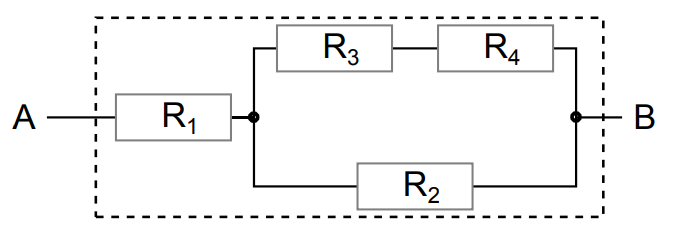
\includegraphics[width=0.5\linewidth]{2012-v3p-06-yl.png}
\end{center}
\fi
}

% Ü8
\ylDisplay{Skeem} % Ülesande nimi
{Tundmatu autor} % Autor
{lõppvoor} % Voor
{2013} % Aasta
{P 2} % Ülesande nr.
{2} % Raskustase
{
% Teema: Elektriõpetus
\ifStatement
Leidke joonisel toodud mõõteriistade näidud. Vooluallika pinge on $U$, kõikide takistite takistused on $R$ ning mõõteriistad on ideaalsed.
\begin{center}
	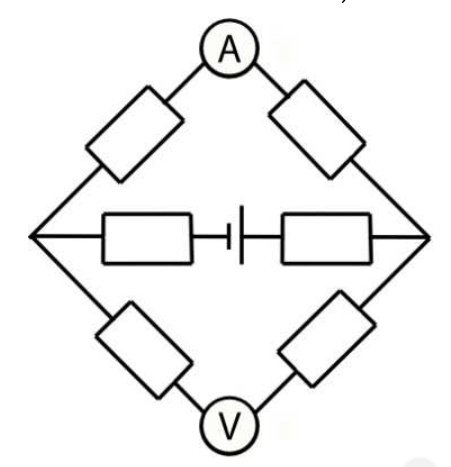
\includegraphics[width=0.5\linewidth]{2013-v3p-02-yl.png}
\end{center}
\fi
}

% Ü9
\ylDisplay{Must kast} % Ülesande nimi
{Tundmatu autor} % Autor
{lõppvoor} % Voor
{2013} % Aasta
{P 5} % Ülesande nr.
{2} % Raskustase
{
% Teema: Elektriõpetus
\ifStatement
Kui joonisel näidatud musta kasti klemmide $A$ ja $B$ külge ühendada patarei pingega $U$ ja klemmide $C$ ja $D$ külge voltmeeter, on voltmeetri näit $U$. Kui ühendada sama patarei klemmide $C$ ja $D$ külge ning voltmeeter klemmide $A$ ja $B$ külge, on voltmeetri näit $U/2$. Teades, et mustas kastis on ainult identsed takistid, joonistage musta kasti skeem!
\begin{center}
	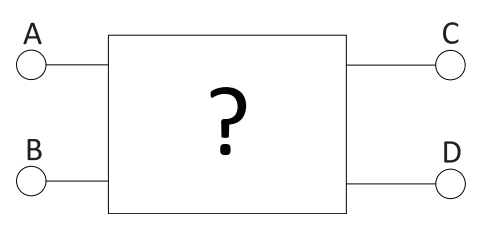
\includegraphics[width=0.5\linewidth]{2013-v3p-05-yl.png}
\end{center}
\fi
}

% Ü10
\ylDisplay{Takistite võimsused} % Ülesande nimi
{Tundmatu autor} % Autor
{lõppvoor} % Voor
{2014} % Aasta
{P 6} % Ülesande nr.
{2} % Raskustase
{
% Teema: Elektriõpetus
\ifStatement
Vooluallikaga muutumatu pingega $U$ ühendati kaks takistit. Kui takistid olid ühendatud jadamisi, oli voolu võimsus vooluringis $2$ W. Kui takistid olid ühendatud rööbiti, oli voolu võimsus vooluringis $9$ W. Arvuta voolu võimsus nendel kahel juhul, kui sama vooluallikaga on ühendatud ainult üks või teine takisti.
\fi
}

% Ü11
\ylDisplay{Elektriskeem} % Ülesande nimi
{Tundmatu autor} % Autor
{lõppvoor} % Voor
{2014} % Aasta
{P 8} % Ülesande nr.
{2} % Raskustase
{
% Teema: Elektriõpetus
\ifStatement
Mitu korda erineb süsteemi maksimaalne ja minimaalne takistus sõltuvalt lülitite asendist? Esimene lüliti saab olla kas asendis $A$ või $B$ ning teine lüliti asendites $C$ või $D$ Kõikide takistite väärtused on $R = 1$ $\Omega$.
\begin{center}
	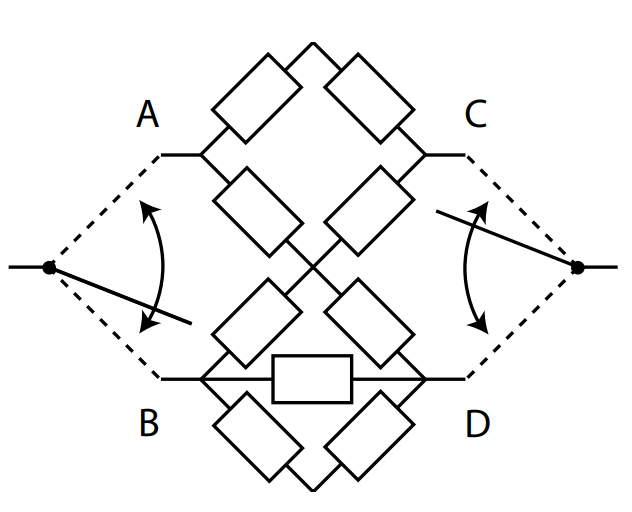
\includegraphics[width=0.5\linewidth]{2014-v3p-08-yl.png}
\end{center}
\fi
}


% Ü12
\ylDisplay{Voltmeeter} % Ülesande nimi
{Tundmatu autor} % Autor
{piirkonnavoor} % Voor
{2016} % Aasta
{P 4} % Ülesande nr.
{2} % Raskustase
{
% Teema: Elektriõpetus
\ifStatement
Voltmeeter on ühendatud joonisel näidatud viisil skeemi, mis koosneb neljast ühesugusest takistist $R$ ning patareist pingega $E = 9$ $V$. Leidke voltmeetri näit.
\begin{center}
	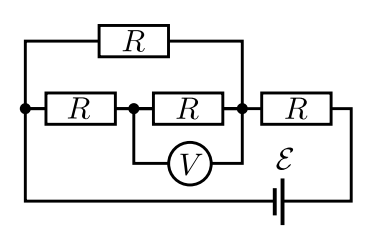
\includegraphics[width=0.5\linewidth]{2016-v2p-04-yl.png}
\end{center}
\fi
}


% Ü13
\ylDisplay{Mõõtepiirkond} % Ülesande nimi
{Tundmatu autor} % Autor
{lõppvoor} % Voor
{2016} % Aasta
{P 3} % Ülesande nr.
{2} % Raskustase
{
% Teema: Elektriõpetus
\ifStatement
Jüri soovis suurendada oma milliampermeetri mõõtepiirkonda. Tema mõõteriista takistus oli $R_A = 3,0$ $\Omega$ ning mõõtepiirkond $0 - 50$ $mA$. Jüri konstureeris uue mõõteriista, ühendades milliampermeetriga rööbiti takisti, mille tegemiseks oli ta kasutanud $s = 2,0$ $mm$ läbimõõduga $l = 20$ $m$ pikkust konstantaantraati, mille eritakistus $\rho = 0,50$ $\frac{\Omega \cdot mm^2}{m}$ . Uue mõõteriistaga voolutugevust mõõtes näitas milliampermeeter $I = 35$ $mA$. Kui suur oli tegelik vool uues mõõteriistas? Kui suur on uue mõõteriista mõõtepiirkond?
\fi
}

% Ü14
\ylDisplay{Juhtmed} % Ülesande nimi
{Tundmatu autor} % Autor
{lõppvoor} % Voor
{2017} % Aasta
{P 4} % Ülesande nr.
{2} % Raskustase
{
% Teema: Elektriõpetus
\ifStatement
Saarevaht saab elamiseks vajaliku elektrienergia katusele paigaldatud päikeseelementidest, mille energia salvestatakse majas asuvasse akusse. Majast kaugusel $l = 50$ $m$ paikneb veinikelder, kuhu saarevaht kogub kaldale uhutud rummipudeleid. Et ka öisel ajal oleks võimalik pudelite etikette selgelt välja lugeda, otsustab saarevaht keldrisse paigaldada hõõglambipirni nimipingega $U = 12$ $V$ ja nimivõimsusega $P = 25$ $W$ ning vedada majast keldrini toitejuhtmed, milleks on saarevahil paraku vaid kasutada valvesüsteemides kasutatav peenike vaskjuhe eritakistusega $\rho = 1,7 \cdot 10^{-8} \cdot m$ ja ristlõikepindalaga $S = 0,20$ $mm^2$. Arvutage, millise võimsusega hakkab põlema keldrisse paigaldatud hõõglamp, kui pinge aku klemmidel on $E = 13$ $V$. Pirni takistuse sõltuvust temperatuurist ei ole vaja arvestada. 
\fi
}

% Ü15
\ylDisplay{Must kast} % Ülesande nimi
{EFO žürii} % Autor
{piirkonnavoor} % Voor
{2019} % Aasta
{P 6} % Ülesande nr.
{2} % Raskustase
{
% Teema: Elektriõpetus
\ifStatement
Kahe väljundklemmiga mustas kastis on mingil viisil ühendatud kolm ühesuguse takistusega takistit ja üks lüliti. Kui mõõta väljundklemmide vahelist takistust, siis sõltuvalt lüliti asendist on tulemuseks kas $15$ $\Omega$ või $20$ $\Omega$. Leidke, kuidas on ühendatud takistid ja lüliti ning milline on takisti takistus.
\fi
}

% Ü16
\ylDisplay{Antikaitse} % Ülesande nimi
{Kaur Aare Saar} % Autor
{piirkonnavoor} % Voor
{2020} % Aasta
{P 9} % Ülesande nr.
{2} % Raskustase
{
% Teema: Elektriõpetus
\ifStatement
Antikaitse (joonisel $AK$) on seade, mis enne aktiveerumist käitub kui avatud lüliti (väga suure takistusega takisti). Kui aga antikaitsele rakendada kõrge pinge, siis see aktiveerub, ning pärast seda käitub jäädavalt kui suletud lüliti. Antikaitsmeid kasutatakse näiteks jadamisi ühendatud jõuluküünaldes, et tagada pärast ühe lambi katkiminekut teiste lampide töötamine. Joonisel on elektriskeem, milles on kokku $n = 16$ jadamisi ühendatud ühesugust küünalt. Pinge skeemi otstel $V = 240$ $V$. Iga küünal on ühendatud rööpselt antikaitsega. Hetkel $t = 0$ küünal $A$ puruneb. Eeldada, et antikaitse aktiveerub, kui sellele on rakendunud pinge, mis on kõrgem kui $21$ $V$ kauemaks kui $\tau = 1$ $ms$, ja et iga küünal on ette nähtud töötama pingel kuni $24$ $V$. Kirjeldage, kuidas muutuvad pinged lampide klemmidel lambi $A$ katkimineku käigus.  Milline on minimaalne lampide arv, mis saavad korraga põleda?
\begin{center}
	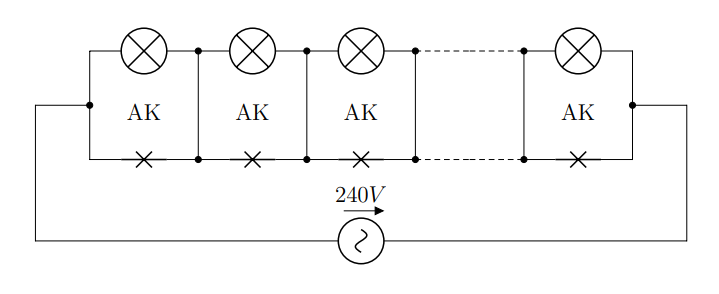
\includegraphics[width=0.5\linewidth]{2020-v2p-09-yl.png}
\end{center}
\fi
}

% Ü17
\ylDisplay{Elektriküünlad} % Ülesande nimi
{Tundmatu autor} % Autor
{piirkonnavoor} % Voor
{2013} % Aasta
{P 7} % Ülesande nr.
{3} % Raskustase
{
% Teema: Elektriõpetus
\ifStatement
Miku ehtis jõulude ajal kuuse elektriküünaldega, milles jadamisi oli ühendatud $20$ lampi nimepingega $12$ $V$ ja nimivõimsusega $15$ $W$. Paari päeva pärast põles uks lampidest läbi. Kuna Mikul samasugust lampi ei olnud, asendas ta läbipõlenud lambi ema õmblusmasina lambiga, mille nimivõimsus oli samuti $15$ $W$, kuid nimipinge $220$ $V$. Mitu korda muutus lambi vahetuse tõttu elektrivoolu võimsus teistes lampides ning millise eredusega põlesid pärast lambi vahetust teised lambid? Pinge elektriküünalde pistiku otstel oli $220$ $V$. Eeldada, et lambi takistus ei sõltu temperatuurist ja pingest.

\ifHint
Esmalt leia valgustite algne tegelik pinge ja võimsus, mis on väiksemad nimipingest ja -võimsusest.
\fi
}

% Ü18
\ylDisplay{Mobiililaadija} % Ülesande nimi
{Tundmatu autor} % Autor
{piirkonnavoor} % Voor
{2014} % Aasta
{P 8} % Ülesande nr.
{3} % Raskustase
{
% Teema: Elektriõpetus
\ifStatement
Leiutajad on pakkunud välja toreda seadme matkainimestele oma telefoni laadimiseks. Ühe saapa talla sisse pannakse mehhanism, mis toimib amortisaatorina. Iga kord kui kannale toetutakse, muundatakse mehaaniline töö väikese elektrigeneraatori abil elektrienergiaks. Oletame, et matkaja mass $m = 60$ $kg$ ja ühe sammu ajal vajub tald kokku $h = 5$ $mm$ võrra. Antud seadme kasutegur $\eta = 0,2$. Matkaja keskmiseks sammupaari pikkuseks ehk kahe järjestikuse samale kannale astumise vahemaaks võtame $d = 1,5$ $m$. Nüüd tuleb vaid ühendada telefon juhtmega saapa külge ja aku laadimine võib alata. Arvestage, et tüüpilises nutitelefonis on liitium-polümeer aku, mis töötab pingel $U = 3,7$ $V$. Samuti arvestage, et kui telefon töötaks keskmisel voolutugevusel $I_k = 130$ $mA$, suudaks aku vastu pidada $T = 10$ tundi. Arvutage, kui pika maa peab matkaja maha kõndima, et tühi telefoni aku uuesti täis laadida.
\fi
}

% Ü19
\ylDisplay{Voltmeeter} % Ülesande nimi
{Tundmatu autor} % Autor
{lõppvoor} % Voor
{2015} % Aasta
{P 3} % Ülesande nr.
{3} % Raskustase
{
% Teema: Elektriõpetus
\ifStatement
 Kui suur on pinge, mida näitab voltmeeter (vt joonis)? Voltmeetri takistus on väga suur. Takistite takistused on vastavalt $R_1 = 15$ $\Omega$, $R_2 = 85$ $\Omega$, $R_3 = 25$ $\Omega$ ja $R_4 = 175$ $\Omega$. Pinge vooluallika klemmidel on $U = 20$ V.
\begin{center}
	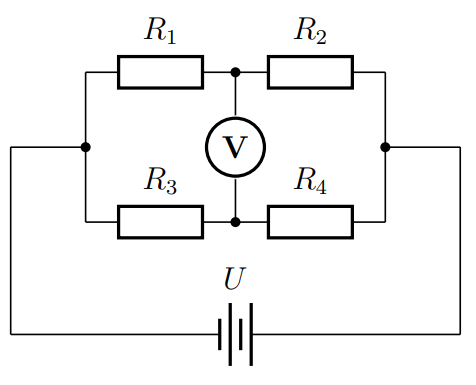
\includegraphics[width=0.5\linewidth]{2015-v3p-03-yl.png}
\end{center}
\fi
}

% Ü20
\ylDisplay{Kaks skeemi} % Ülesande nimi
{Tundmatu autor} % Autor
{lõppvoor} % Voor
{2015} % Aasta
{P 6} % Ülesande nr.
{3} % Raskustase
{
% Teema: Elektriõpetus
\ifStatement
Antud on kaks elektriskeemi (vt joonis), mis erinevad ühe takisti takistuse ja patarei pinge väärtuste poolest. Teada on, et mõlemal skeemil läbib takistit R sama suur vool, kuid esimesel on takistit R1 läbiva voolu tugevus kaks korda suurem kui takistit $3R$ läbiva voolu tugevus ja teisel takistit $R2$ läbiva voolu tugevus viis korda suurem kui takistit $3R$ läbiva voolu tugevus. Leida, kumma patarei pinge on suurem ning kui mitu korda.
\begin{center}
	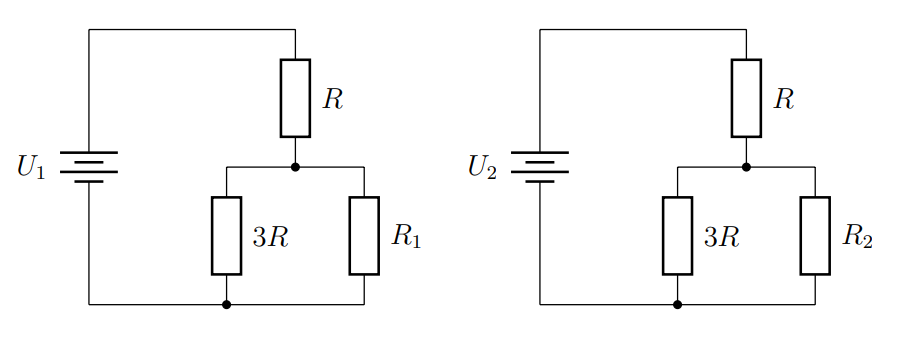
\includegraphics[width=0.5\linewidth]{2015-v3p-06-yl.png}
\end{center}
\fi
}

% Ü21
\ylDisplay{Kaheksa} % Ülesande nimi
{Tundmatu autor} % Autor
{lõppvoor} % Voor
{2016} % Aasta
{P 9} % Ülesande nr.
{3} % Raskustase
{
% Teema: Elektriõpetus
\ifStatement
Juku paigutab takisteid takistusega $R$ number $8$ kuju järgi, nagu näidatud joonisel. Kõik takistid, millel on üks ühine punkt, on elektriliselt ühendatud. Juku mõõdab kõikvõimalike punktide vahel takistust. Millise vähima väärtuse ja milliste punktide vahel ta saab? Lahenduses vaadake läbi kõik võimalikud juhud. 
\begin{center}
	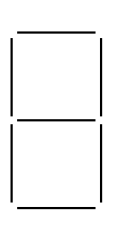
\includegraphics[width=0.5\linewidth]{2016-v3p-09-yl.png}
\end{center}
\fi
}

% Ü22
\ylDisplay{Jõulutuled} % Ülesande nimi
{EFO žürii} % Autor
{piirkonnavoor} % Voor
{2017} % Aasta
{P 8} % Ülesande nr.
{3} % Raskustase
{
% Teema: Elektriõpetus
\ifStatement
Jüri jõulukuuse valgustus koosnes 20 lambist. Iga lamp oli arvestatud pingele $12$ V ning võimsuseks oli $1$ W. Jõuluõhtul põles üks lampidest läbi ning kogu jõulukuuse valgustus kustus. Jüri leidis kiiresti riknenud lambi, kuid uut sellist tema sahtlites ei olnud. Küll leidis ta aga oma sahtlitest kaks sama välimusega lampi, mis mõlemad oli arvestatud pingele $24$ V. Ühe lambi võimsuseks oli $1$ W, teise lambi võimsuseks $5$ W. Jüri arvutas veidi ning keeras pesasse ühe lampidest. Kumma lambi ta kasutusele võttis, et kuuse valgustus säraks peaaegu sama kaunilt (võimalikult sarnase võimsusega) kui enne ühe lambi läbipõlemist? Pinge Jüri korteri seinakontaktis on $240$ V. Lampide takistuse sõltuvust temperatuurist pole tarvis arvestada. Lisa Jüri valiku põhjendus.
\fi
}

% Ü23
\ylDisplay{Takistid} % Ülesande nimi
{Tundmatu autor} % Autor
{lõppvoor} % Voor
{2017} % Aasta
{P 8} % Ülesande nr.
{3} % Raskustase
{
% Teema: Elektriõpetus
\ifStatement
Leidke takistus punktide $A$ ja $B$ vahel. Iga takisti takistus on $R$.
\begin{center}
	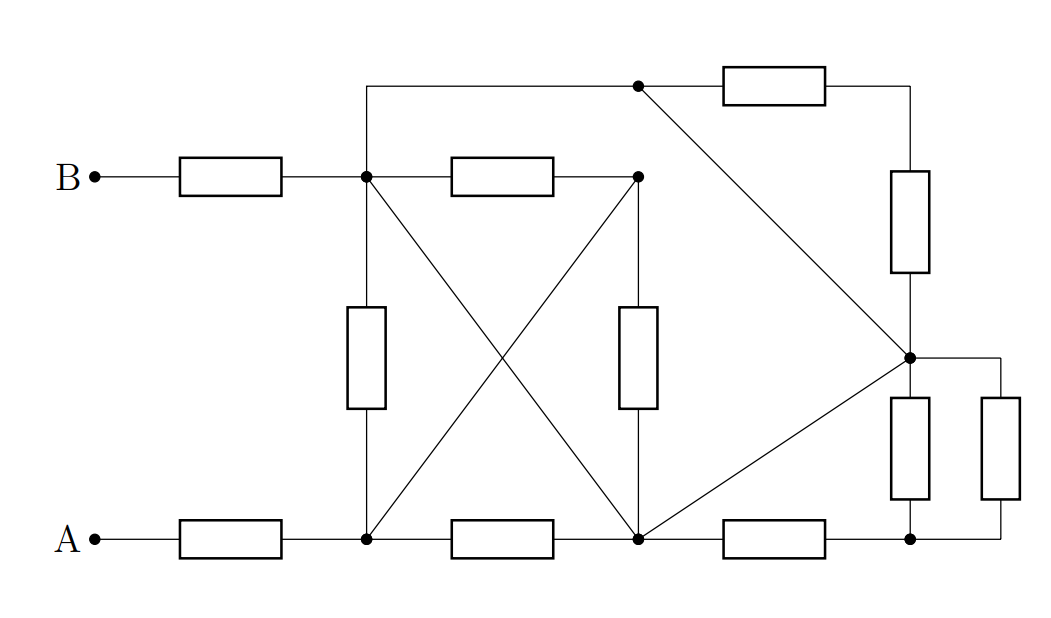
\includegraphics[width=0.5\linewidth]{2017-v3p-08-yl.png}
\end{center}
\fi
}

% Ü24
\ylDisplay{Pinge mõõtmine} % Ülesande nimi
{Tundmatu autor} % Autor
{lõppvoor} % Voor
{2017} % Aasta
{P 9} % Ülesande nr.
{3} % Raskustase
{
% Teema: Elektriõpetus
\ifStatement
Kolm takistit väärtustega $R_1 = 5000$ $\Omega$, $R_2 = 3000$ $\Omega$ ja $R_3 = 1000$ $\Omega$ on ühendatud jadamisi. Pinge takistite jada otstel on $U = 100$ $V$. Mõõtes voltmeetriga pinget takisti $R_2$ klemmidel, saadi pinge väärtuseks $U_2 = 23,8$ $V$. Kui suurt pinget näitab sama voltmeeter siis, kui see ühendada takisti $R_1$ klemmidega?
\fi
}

% Ü25
\ylDisplay{Takisti} % Ülesande nimi
{Jonathan Kalmus} % Autor
{piirkonnavoor} % Voor
{2018} % Aasta
{P 6} % Ülesande nr.
{3} % Raskustase
{
% Teema: Elektriõpetus
\ifStatement
Juku tahab mõõta tundmatu takisti väärtust. Selleks ühendab ta takistiga rööbiti voltmeetri ning ampermeetri jadamisi nagu näidatud joonisel. Ampermeetri näit $I = 15$ $m_A$ ning voltmeetri näit $U = 5$  $V$. Voltmeetri takistus $R_V = 1000$ $\Omega$. Leidke tundmatu takisti väärtus.
\begin{center}
	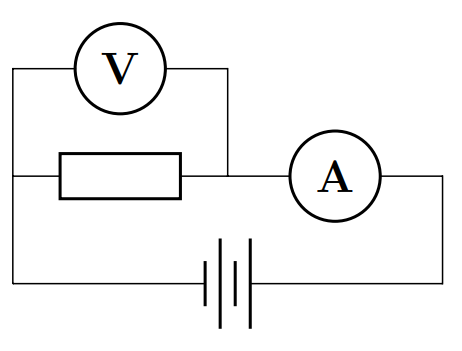
\includegraphics[width=0.5\linewidth]{2018-v2p-06-yl.png}
\end{center}
\fi
}

% Ü26
\ylDisplay{Päikesepaneelid} % Ülesande nimi
{Jonathan Kalmus} % Autor
{lõppvoor} % Voor
{2018} % Aasta
{P 3} % Ülesande nr.
{3} % Raskustase
{
% Teema: Elektriõpetus
\ifStatement
Vasakpoolsel joonisel on toodud ühe päikesepaneeli tootmisvõimsus ööpäeva lõikes ning parempoolsel joonisel linna tarbimisvõimsus ööpäeva lõikes. Hinnata, mitu taolist päikesepaneeli on vaja, et katta kogu linna energiavajadus ööpäeva jooksul. Kui suur peab olema minimaalselt linna energiamahuti, et ööpäevast kõikumist tootmise ja tarbimise vahel kompenseerida?
\begin{center}
	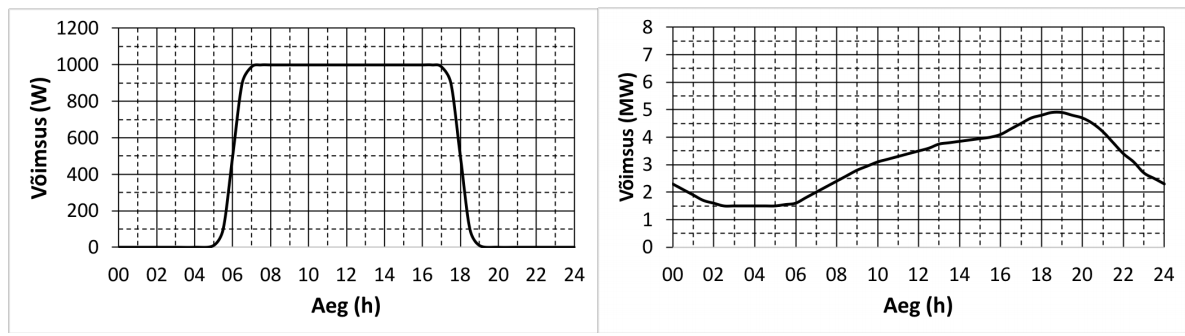
\includegraphics[width=0.5\linewidth]{2018-v3p-03-yl.png}
\end{center}
\fi
}

% Ü27
\ylDisplay{Vooluring} % Ülesande nimi
{Koit Timpmann} % Autor
{lõppvoor} % Voor
{2018} % Aasta
{P 7} % Ülesande nr.
{3} % Raskustase
{
% Teema: Elektriõpetus
\ifStatement
Vooluringis on neli takistit väärtustega $R_1 = 2 \Omega$, $R_2 = 3 \Omega$, $R_3 = 6 \Omega$ ja $R_4 = 7 \Omega$. Punktide $C$ ja $D$ vahel on juhe, mille takistus on $0 \Omega$. Punktide $A$ ja $B$ vahele on rakendatud pinge suurusega $U = 18$ $V$. Kui suur on voolutugevus juhtmes $CD$?
\begin{center}
	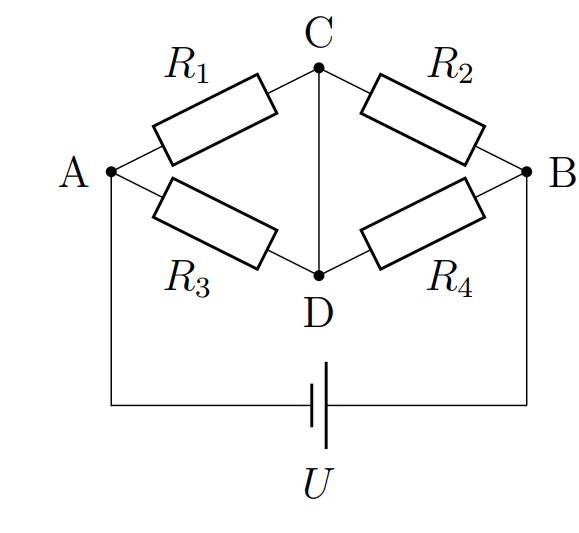
\includegraphics[width=0.5\linewidth]{2018-v3p-07-yl.png}
\end{center}
\fi
}

% Ü28
\ylDisplay{Elektriskeem} % Ülesande nimi
{EFO žürii} % Autor
{piirkonnavoor} % Voor
{2019} % Aasta
{P 7} % Ülesande nr.
{3} % Raskustase
{
% Teema: Elektriõpetus
\ifStatement
Kõigi vooluringis olevate takistite takistus on sama suur. Kui suur on takisti takistus, kui vooluallika pinge $U = 3$ $V$ korral näitab ampermeeter voolutugevuseks $I = 1$ $A$.
\begin{center}
	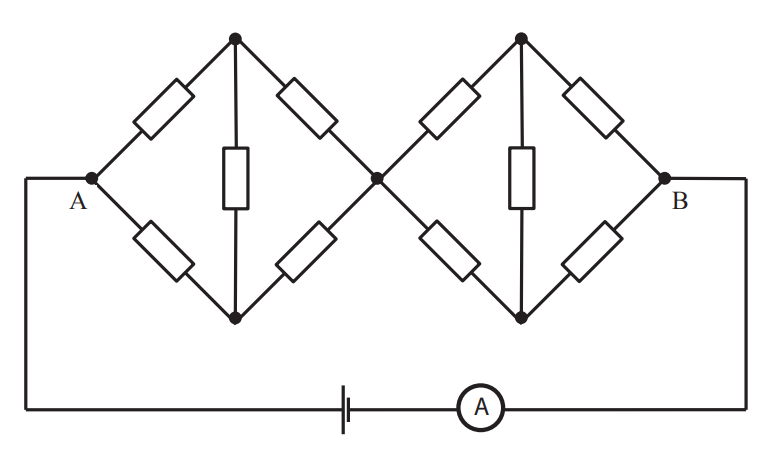
\includegraphics[width=0.5\linewidth]{2019-v2p-07-yl.png}
\end{center}
\fi
}

% Ü29
\ylDisplay{Kontuuri takistus} % Ülesande nimi
{Koit Timpmann} % Autor
{lõppvoor} % Voor
{2019} % Aasta
{P 7} % Ülesande nr.
{3} % Raskustase
{
% Teema: Elektriõpetus
\ifStatement
Kõrvaloleval joonisel esitatud kujund on valmistatud ühesugusest traadist. Kujundi diameetri pikkuse traadijupi elektriline takistus $R = 1$ $\Omega$. Kui suur on vooltugevus kujundi diameetris $AC$, kui pinge punktide $A$ ja $B$ vahel $U = 1,5$ $V$. 
\begin{center}
	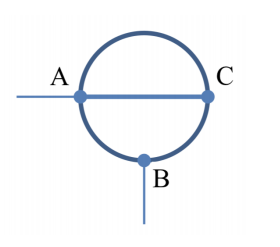
\includegraphics[width=0.5\linewidth]{2019-v3p-07-yl.png}
\end{center}
\fi
}

% Ü30
\ylDisplay{Mikrokuumuti} % Ülesande nimi
{Valter Kiisk} % Autor
{lõppvoor} % Voor
{2019} % Aasta
{P 9} % Ülesande nr.
{3} % Raskustase
{
% Teema: Elektriõpetus
\ifStatement
Mikrokuumuti kujutab endast miniatuurset küttekeha, mis on kantud elektrit mittejuhtiva alusmaterjali pinnale. Küttekeha takistus toatemperatuuril $(t_0 = 20$ $^{\circ}C)$ $R_0 = 50$ $\Omega$. Pärast pinge $U_1 = 1$ $V$ rakendamist saadi voolutugevuseks $I_1 = 12$ $mA$ ning kuumuti temperatuur saavutas väärtuse $t_1 = 420$ $^{\circ}C$. Küttekeha takistus selles temperatuurivahemikus sõltub lineaarselt temperatuurist, st $R_t = R_0 [1 + \alpha (t - t_0)]$, kus $\alpha$ on konstant. Eeldage, et soojuskadude võimsuse on võrdeliseks küttekeha temperatuuri ja toatemperatuuri vahega, st $P_t = k(t - t_0)$, kus $k$ on konstant. 
1) Leidke konstantide $\alpha$ ja $k$ väärtused. 
2) Hinnake võimalikult täpselt kuumuti temperatuur pingel $U = 0,7$ $V$.
\fi
}
\newpage\subsection{\protect\StrSubstitute{Mehaanika}{-}{ }}

% Ü31
\ylDisplay{Trepp} % Ülesande nimi
{Tundmatu autor} % Autor
{lõppvoor} % Voor
{2011} % Aasta
{P 1} % Ülesande nr.
{1} % Raskustase
{
% Teema: Mehaanika
\ifStatement
Juku kõndis vanaema Juulaga trepist üles. Juku kõndis trepist üles kiirusega $v_1$ (korrust/minutis). Kui ta jõudis viiendale korrusele, siis hakkas ta alla tulema kiirusega $v_2$. Juku ja vanaema kohtusid teisel korrusel. Mitmendale korrusele jõuaks Juku ajaga, mis vanaemal kulub viiendale korrusele minekuks? Juku liigub trepist alla kaks korda kiiremini kui üles. Maja esimene korrus asus maapinnal.
\fi
}


% Ü32
\ylDisplay{Liikumine} % Ülesande nimi
{Autor} % Autor
{lõppvoor} % Voor
{2011} % Aasta
{P 2} % Ülesande nr.
{1} % Raskustase
{
% Teema: Mehaanika
\ifStatement
Graafikul on kujutatud liikuva keha kiiruse sõltuvust ajast. Kui suur oli vaadeldava aja jooksul keha suurim kaugus algasendist? Kui kaugel oli keha algasendist vaadeldava ajavahemiku lõpus?
\begin{center}
	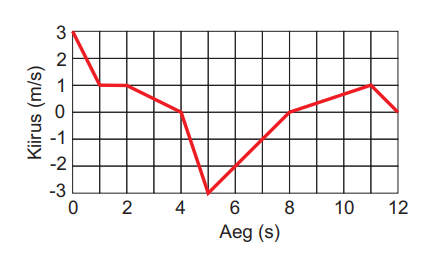
\includegraphics[width=0.5\linewidth]{2011-v3p-02-yl.PNG}
\end{center}
\fi
}



% Ü33
\ylDisplay{Võidusõiduautod} % Ülesande nimi
{Tundmatu autor} % Autor
{piirkonnavoor} % Voor
{2012} % Aasta
{P 6} % Ülesande nr.
{1} % Raskustase
{
% Teema: Mehaanika
\ifStatement
Võidusõiduauto keskmine kiirus ringrajal peetud treeningu jooksul oli $v = 50$ $m/s$. Kui arvutati peale esimese ja teise kõikide ulejäänud sõidetud ringide keskmine kiirus, leiti, et see oli täpselt sama, $50$ $m/s$. Esimese ringi läbimiseks kulus aega $t_1 = 107$ $s$. Kui palju aega kulus teise ringi läbimiseks? Ühe ringi pikkus oli $l = 5150$ $m$.
\fi
}


% Ü34
\ylDisplay{Golfilöök} % Ülesande nimi
{Tundamtu autor} % Autor
{lõppvoor} % Voor
{2012} % Aasta
{P 2} % Ülesande nr.
{1} % Raskustase
{
% Teema: Mehaanika
\ifStatement
Sarivõttega pildistati golfimängijat nii, et iga kahe pildi vahel oli ajavahemik $\tau = 16$ ms. Hinnake golfipalli algkiirust joonise abil. Pall liigub risti vaatesuunaga. Allpool on pilt.
\begin{center}
	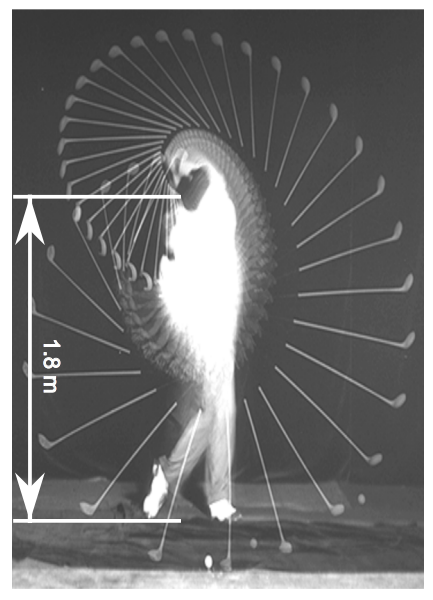
\includegraphics[width=0.5\linewidth]{2012-v3p-02-yl.PNG}
\end{center}
\fi
}


% Ü35
\ylDisplay{Jõe ületamine} % Ülesande nimi
{Tundmatu autor} % Autor
{piirkonnavoor} % Voor
{2014} % Aasta
{P 1} % Ülesande nr.
{1} % Raskustase
{
% Teema: Mehaanika
\ifStatement
Paat sõitis üle jõe, mille laius oli $d = 120$ m, nii, et paadi siht oli kogu aeg risti jõega. Kui suur pidi olema paadi keskmine kiirus jõevoolu suhtes, kui on teada, et paadi maabumiskoht teisel kaldal asetses $s = 12$ m lähtekohast allavoolu? Vee voolukiirus jões oli $u = 0,8$ m/s.
\fi
}

% Ü36
\ylDisplay{Ringrada} % Ülesande nimi
{Tundmatu autor} % Autor
{lõppvoor} % Voor
{2014} % Aasta
{P 1} % Ülesande nr.
{1} % Raskustase
{
% Teema: Mehaanika
\ifStatement
Juhan, Kalle ning Lauri sõidavad ringrajal jalgratastega võidu. Kõik kolm stardivad korraga ühest kohast ning iga rattur sõidab muutumatu kiirusega. On teada, et Kalle teeb Juhanile ringi sisse siis, kui Kalle on just lõpetanud viienda ringi. Lauri teeb Kallele ringi sisse siis, kui Lauri on just lõpetanud kuuenda ringi. Mitu ringi oli Juhan sõitnud, kui Lauri temast esimest korda ringiga möödus?
\fi
}



% Ü37
\ylDisplay{Laua lükkamine} % Ülesande nimi
{Autor} % Autor
{lõppvoor} % Voor
{2014} % Aasta
{P 2} % Ülesande nr.
{1} % Raskustase
{
% Teema: Mehaanika
\ifStatement
 Mees hoiab ühest otsast lauda, mille teine ots lebab külili maa peal oleval tühjal vaadil. Laua lükkamisel hakkab vaat pöörlema ja liikuma mööda horisontaalset maapinda. Vaat maapinnal ei libise, samuti ei libise ka laud vaadil. Kui pika maa peab maha kõndima lauda lükkav mees, et jõuda vaadini? Laua pikkus on $6$ meetrit.
\begin{center}
	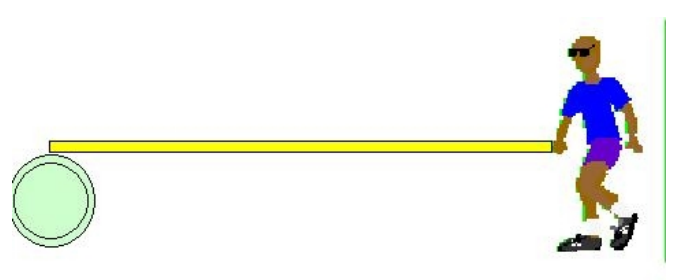
\includegraphics[width=0.5\linewidth]{2014-v3p-02-yl.PNG}
\end{center}
\fi
}


% Ü38
\ylDisplay{Helilaine} % Ülesande nimi
{Tundmatu autor} % Autor
{lõppvoor} % Voor
{2015} % Aasta
{P 1} % Ülesande nr.
{1} % Raskustase
{
% Teema: Mehaanika
\ifStatement
Rõngas on kokku keevitatud kahest eri metallist poolrõngast. Rõnga raadius on $R$. Heli levib ühes metallis kiirusega $v_1$ ja teises metallis kiirusega $v_2$. Kui suure ajavahemiku pärast kohtuvad helilained, mis tekitatakse haamrilöögiga ühe keevituskoha pihta?
\fi
}

% Ü39
\ylDisplay{Kera vees} % Ülesande nimi
{Autor} % Autor
{lõppvoor} % Voor
{2015} % Aasta
{P 2} % Ülesande nr.
{1} % Raskustase
{
% Teema: Mehaanika
\ifStatement
 Kausis on vesi ja selles kera, mis puudutab põhja. Vett on kausis nii palju, et pool kerast on veest väljas. Kera mõjub põhjale jõuga, mis võrdub $\frac{1}{3}$ kera raskusjõust. Kui suur on kera aine tihedus? Vee tihedus on $\rho = 1,0$ $g/cm^3$.
\fi
}

% Ü40
\ylDisplay{Rong} % Ülesande nimi
{Tundmatu autor} % Autor
{piirkonnavoor} % Voor
{2016} % Aasta
{P 2} % Ülesande nr.
{1} % Raskustase
{
% Teema: Mehaanika
\ifStatement
Jaamast sõitu alustanud kaubarong kiirendas ühtlaselt ja saavutas $t_1=15$ minutiga kiiruse $v=80$ $km/h$. Sõitnud $t_2 = 2,5$ tundi ühtlase kiirusega, hakkas ta pidurdama ja ühtlaselt kiirust vähendades peatus $t_3=10$ minuti pärast järgmises jaamas. Kui suur oli rongi keskmine kiirus jaamadevahelisel teel?
\fi
}

% Ü41
\ylDisplay{Kaheksa} % Ülesande nimi
{EFO žürii} % Autor
{piirkonnavoor} % Voor
{2018} % Aasta
{P 2} % Ülesande nr.
{1} % Raskustase
{
% Teema: Mehaanika
\ifStatement
 Kaheksakujulisel ringrajal alustavad kaks drooni võidusõitu ringide ühenduskohast nooltega $A$ ja $B$ näidatud suundades. Mõlema drooni trajektoorid on kaheksakujulised. Kaheksa ülemise osa pikkus on $l_A = 60$ $m$ ning alumise osa pikkus $l_B = 200$ $m$. Mõlemad droonid lendavad kogu aeg ühtlase kiirusega. Esimese drooni kiirus on $v_A = 10$ $m/s$ ning teise drooni kiirus $v_B = 8$ $m/s$. Kui suure teepikkuse $s$ on läbinud droon $A$, kui droonid uuesti kohtuvad? 
\begin{center}
	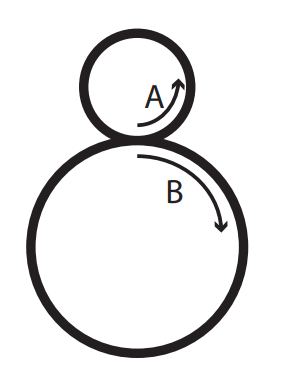
\includegraphics[width=0.5\linewidth]{2018-v2p-02-yl.PNG}
\end{center}
\fi
}


% Ü42
\ylDisplay{Rongid} % Ülesande nimi
{EFO žürii} % Autor
{piirkonnavoor} % Voor
{2019} % Aasta
{P 1} % Ülesande nr.
{1} % Raskustase
{
% Teema: Mehaanika
\ifStatement
Kahe linna vaheline kaugus mööda raudteed on $900$ km. Linnast $A$ väljub kell $22$ kaubarong linna $B$ suunas. Kaubarong sõidab ühtlase kiirusega $90$ km/h. Kolm tundi pärast väljumist teeb rong ühes jaamas pooletunnise peatuse, et lasta endast mööda kiirrong. Pärast seda jätkab kaubarong sõitu endise kiirusega. Kaks tundi pärast kaubarongi väljumist väljub linnast $B$ kiirrong linna $A$ suunas. Kiirrong liigub peatusteta keskmise kiirusega $144$ km/h. Mis kell ja kui kaugel jaamast $A$ rongid kohtuvad?  
\fi
}

% Ü43
\ylDisplay{Päästerõngas} % Ülesande nimi
{EFO žürii} % Autor
{lõppvoor} % Voor
{2020} % Aasta
{P 1} % Ülesande nr.
{1} % Raskustase
{
% Teema: Mehaanika
\ifStatement
Juku tahtis kontrollida oma füüsikaalaste teadmiste õigsust. Ta leppis kokku isa ja tolle sõbraga, et nad sõidaksid paatidega suhteliselt pikal sirgel jõelõigul teineteisele vastu muutumatute kiirustega. Kohtumise hetkel visatakse kummastki paadist välja päästerõngas, sõidetakse edasi täpselt $3$ minutit, siis pööratakse ümber ja jätkatakse sõitu mootori sama võimsusega. Kumb paatidest jõuab enne päästerõngani? Esialgu vastuvoolu sõitva paadi kiiruseks on kohtumise hetkel $12$ km/h ja allavoolu sõitva paadi kiiruseks $20$ km/h.
\fi
}


% Ü44
\ylDisplay{Varras} % Ülesande nimi
{Tundmatu autor} % Autor
{lõppvoor} % Voor
{2011} % Aasta
{P 4} % Ülesande nr.
{2} % Raskustase
{
% Teema: Mehaanika
\ifStatement
Sirge ühtlane varras on ühest otsast jäigalt kinnitatud. Kui varda vabale otsale rakendatakse risti vardaga jõud $F_0$, murdub varras kinnituskohast. Nüüd asetatakse kaks korda pikema varda mõlemad otsad tugedele ning varda keskkohale hakatakse risti vardaga jõudu rakendama. Millise jõu $F$ korral ja kustkohast murdub varras seekord?
\fi
}


% Ü45
\ylDisplay{Lauatennisepall} % Ülesande nimi
{Tundmatu autor} % Autor
{lõppvoor} % Voor
{2011} % Aasta
{P 5} % Ülesande nr.
{2} % Raskustase
{
% Teema: Mehaanika
\ifStatement
Lauatennisepall läbimõõduga $d = 30$ mm ja massiga $m = 5$ g suruti vette sügavusele $H = 30$ cm. Kui pall sel sügavusel lahti lasti, hüppas see veest välja kõrgusele $h = 10$ cm. Kui palju energiat muundus siseenergiaks palli ja vee hõõrdumise tõttu? Hõõrdumist õhuga lugeda tühiseks, vee tihedus $\rho_v = 1000$ $kg/m^3$.
\fi
}

% Ü46
\ylDisplay{Kolksatused} % Ülesande nimi
{Tundmatu autor} % Autor
{piirkonnavoor} % Voor
{2012} % Aasta
{P 5} % Ülesande nr.
{2} % Raskustase
{
% Teema: Mehaanika
\ifStatement
Raudteerööbas on $25$ $m$ pikk. Kui pika aja vältel tuleks lugeda vaguni ühe telje rataste kolksatusi, et nende arv võrduks vaguni kiirusega kilomeetrites tunnis?
\fi
}


% Ü47
\ylDisplay{Tünn} % Ülesande nimi
{Tundmatu autor} % Autor
{piirkonnavoor} % Voor
{2012} % Aasta
{P 7} % Ülesande nr.
{2} % Raskustase
{
% Teema: Mehaanika
\ifStatement
Vees ujuva tühja plekktünni ruumalast on $\frac{1}{10}$ vee sees. Pärast tünni täitmist tundmatu vedelikuga jääb tünn vee peale ujuma, kuid nüüd on vee sees $\frac{9}{10}$ tünni ruumalast. Kui suur on tünni valatud vedeliku tihedus? Vee tihedus on $1000 \frac{kg}{m3}$.
\fi
}

% Ü48
\ylDisplay{Koer} % Ülesande nimi
{Tundmatu autor} % Autor
{lõppvoor} % Voor
{2012} % Aasta
{P 4} % Ülesande nr.
{2} % Raskustase
{
% Teema: Mehaanika
\ifStatement
Poiss on koos oma koeraga rannas. Joonisel kujutatud hetkel kutsub ta koera enda juurde, kuid koer soovib teel poisi juurde korraks ka veest läbi hüpata. Millise minimaalse ajaga jõuab ta sel juhul poisini? Koer jookseb kiirusega $v = 4,0$ m/s.
\begin{center}
	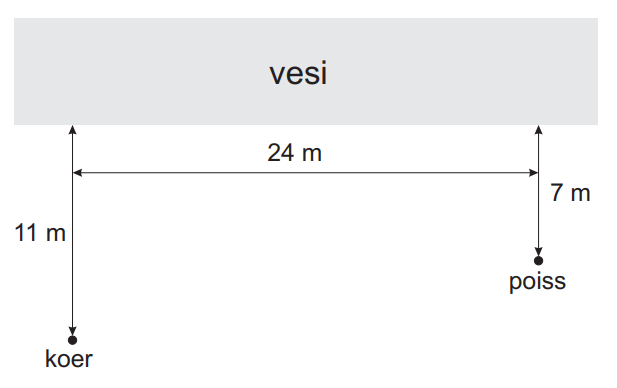
\includegraphics[width=0.5\linewidth]{2012-v3p-04-yl.PNG}
\end{center}
\fi
}

% Ü49
\ylDisplay{Ujuv anum} % Ülesande nimi
{Tundmatu autor} % Autor
{lõppvoor} % Voor
{2013} % Aasta
{P 1} % Ülesande nr.
{2} % Raskustase
{
% Teema: Mehaanika
\ifStatement
Risttahukakujulisse anumasse põhja pindalaga $S_1$ asetatakse ujuma väiksem risttahukakujuline anum põhjapindalaga $S_2$. Selle tulemusel tõusis veetase suures anumas kõrguse $\triangle h$ võrra. Siis hakati väiksemasse anumasse vett valama. Milline on minimaalne kaugus väiksemas anumas oleva vee pinna ja väikese anuma ääre vahel nii, et see veel ei upuks? 
\fi
}

% Ü50
\ylDisplay{Bussid} % Ülesande nimi
{Tundmatu autor} % Autor
{lõppvoor} % Voor
{2013} % Aasta
{P 3} % Ülesande nr.
{2} % Raskustase
{
% Teema: Mehaanika
\ifStatement
Jalgrattur Rein tegi maantee ääres trenni. Mööda teed tulid talle vastu bussid, mis lahkusid algpeatusest iga $15$ minuti tagant. Vähemalt mitu bussi tuli Reinule treeningu jooksul vastu, kui ta sõitis $30$ $km/h$ ja läbis 120 km? Busside sõidukiirus oli $90$ km/h.
\fi
}

% Ü51
\ylDisplay{Parv} % Ülesande nimi
{Tundmatu autor} % Autor
{piirkonnavoor} % Voor
{2014} % Aasta
{P 5} % Ülesande nr.
{2} % Raskustase
{
% Teema: Mehaanika
\ifStatement
Tiigivees asetseb männipuidust parv pindalaga $S = 3$ $m^2$ . Parvel lamab inimene massiga $m = 70$ kg. Arvutage parve paksus, kui on teada, et parve ülemine äär on täpselt tasa veepinnaga. Vee ning männipuidu tihedused on vastavalt $\rho_v = 1000$ $kg/m^3$ ja $\rho_m = 400$ $kg/m3$.
\fi
}

% Ü52
\ylDisplay{Püstolkuulipilduja} % Ülesande nimi
{Tundmatu autor} % Autor
{piirkonnavoor} % Voor
{2014} % Aasta
{P 7} % Ülesande nr.
{2} % Raskustase
{
% Teema: Mehaanika
\ifStatement
Korraldati katse, milles mõõdeti püstolkuulipilduja kuulide keskmist kiirust ja laskude arvu minutis. Selleks sõitsid kahel paralleelsel raudteel vastassuunas rongid. Rong, millest tulistati, sõitis katse ajal muutumatu kiirusega $72$ km/h ja rong, mis oli märklauaks, muutumatu kiirusega $36$ km/h. Rongide kaugus teineteisest oli $60$ m. Esimene lask tehti hetkel, kui rongiga risti oleva püstolkuulipilduja toru ots oli täpselt vastakuti teisele rongile joonistatud märgiga. Kuuliaukude asukohtade mõõtmisel täheldati, et esimene kuul oli tabanud rongi $2,25$ m märgist eemal ja kõikide teiste kuuliaukude kaugus üksteisest oli $2,5$ m. Kui suur on püstolkuulipilduja kuuli lennukiirus ja mitu lasku teeb püstolkuulipilduja minutis?
\fi
}

% Ü53
\ylDisplay{Liiklusummik} % Ülesande nimi
{Tundmatu autor} % Autor
{lõppvoor} % Voor
{2014} % Aasta
{P 4} % Ülesande nr.
{2} % Raskustase
{
% Teema: Mehaanika
\ifStatement
Autod seisavad punase fooritule taga tiheda kolonnina, kus kahe järjestikuse auto esiotste vaheline kaugus on keskmiselt $l_0 = 6$ m ning autode rivi pikkus $L_0 = 150$ m. Peale rohelise tule süttimist hakkavad autod järjest liikuma ning saavutavad kiiruse $v = 50$ km/h. Kiiruse $v$ saavutanud autode esiotste vaheline kaugus $l = 30$ m. Lihtsuse mõttes jätke arvestamata autode kiirendamisele kuluv aeg. Kui kaua alates rohelise tule süttimisest peab viimane auto ootama, enne kui saab liikuma hakata? Kas ta jõuab üle ristmiku juba esimese rohelise tulega või peab uuesti punase tule taha ootama jääma? Rohelise tule kestus on $t = 1$ min. 
\fi
}

% Ü54
\ylDisplay{Töö} % Ülesande nimi
{Tundmatu autor} % Autor
{piirkonnavoor} % Voor
{2016} % Aasta
{P 3} % Ülesande nr.
{2} % Raskustase
{
% Teema: Mehaanika
\ifStatement
Mingi töö tegemiseks kasutati järjestikku kahte seadet. Esimese seadmega tehti ära $25$ \% kogu tööst, ülejäänud töö tehti seadmega, mille võimsus oli $N_2$ $= 2000$ W. Arvutus naitas, et kahe seadme keskmine võimsus kogu töö tegemisel oli olnud $N = 1600$ W. Kui suure osa kogu tööajast töötati esimese seadmega ja kui suur oli selle voimsus $N_1$?
\fi
}

% Ü55
\ylDisplay{Lennuk} % Ülesande nimi
{Tundmatu autor} % Autor
{lõppvoor} % Voor
{2016} % Aasta
{P 2} % Ülesande nr.
{2} % Raskustase
{
% Teema: Mehaanika
\ifStatement
Lennuk lendab otsejoones linnast $A$ linna $B$. Millisel juhul läbib lennuk linnadevahelise vahemaa edasi-tagasi kiiremini ja mitu korda? Esimesel juhul puhub linna $B$ poolt linna $A$ suunas tuul kiirusega $90$ $km/h$ ja teisel juhul puhub sama kiirusega tuul risti linnadevahelise sihiga. Kui tuult ei ole, lendab lennuk ühtlase kiirusega $400$ $km/h$. Mõlemal juhul arvestage ainult lennuaega.
\fi
}

% Ü56
\ylDisplay{Rehvid} % Ülesande nimi
{EFO žürii} % Autor
{piirkonnavoor} % Voor
{2017} % Aasta
{P 1} % Ülesande nr.
{2} % Raskustase
{
% Teema: Mehaanika
\ifStatement
Jüri autole olid ette nähtud $15$-tollised veljed, mille rehvi läbimõõt on $627$ mm. Jüri armastas uhkeldada ja kui tuli aeg autole uued rehvid osta, ostis ta oma autole $16$-tollised veljed, mille rehvi läbimõõt on $652$ mm. Mitme sekundi võrra muutub uute rehvidega $1$ km läbimise aeg, kui auto sõidab spidomeetri järgi kiirusega $90$ km/h? Auto spidomeeter mõõdab kiirust auto ratta pöörete järgi. 
\fi
}

% Ü57
\ylDisplay{Ujumine kanalis} % Ülesande nimi
{EFO žürii} % Autor
{piirkonnavoor} % Voor
{2017} % Aasta
{P 3} % Ülesande nr.
{2} % Raskustase
{
% Teema: Mehaanika
\ifStatement
Voolava veega kanalis on esimene pool kaks korda laiem kui teine pool. Kanali pikkus on $l$ ning sügavus on igal pool sama. Pärivoolu ujudes läbib Juku kanali esimese poole ajaga $t_1$ ning teise poole ajaga $t_2$. Milline on Juku ujumiskiirus $v$ seisvas vees?
\fi
}

% Ü58
\ylDisplay{Kuulikesed} % Ülesande nimi
{EFO žürii} % Autor
{piirkonnavoor} % Voor
{2017} % Aasta
{P 5} % Ülesande nr.
{2} % Raskustase
{
% Teema: Mehaanika
\ifStatement
Kangkaalu otstes asuvad ühesugused anumad. Üks anum täidetakse ääreni väikeste vasest kuulikestega ning teine sama suurte kaadmiumist kuulikestega. Kui kaadmiumist kuulikestega anum täidetakse ääreni veega, on kangkaal tasakaalus. Leidke, millise osakaalu $k$ moodustavad kuulikesed anuma koguruumalast k = Vk/Vanum . Vee tihedus $\rho_v = 1,0$ $g/cm^3$, vase tihedus $\rho_{Cu} = 9,0$ $g/cm^3$ , kaadmiumi tihedus $\rho_{Cd} = 8,6$ $g/cm^3$.
\fi
}

% Ü59
\ylDisplay{Rongid} % Ülesande nimi
{Autor} % Autor
{lõppvoor} % Voor
{2017} % Aasta
{P 3} % Ülesande nr.
{2} % Raskustase
{
% Teema: Mehaanika
\ifStatement
Kiirusega $v_1 = 144$ km/h liikuva reisirongi juht nägi $l = 200$ m kaugusel enda ees samal rööpapaaril liikuvat kaubarongi, mis liikus kiirusega $v_2 = 72$ km/h. Otsasõidu vältimiseks hakkas juht reisirongi ühtlaselt pidurdama, nii et iga sekundi jooksul vähenes rongi kiirus $v = 1$ m/s võrra. Kui kaugel kohast, kus reisirongi vedurijuht märkas kaubarongi, jõuab reisirong kaubarongile järele? Kas selliselt pidurdades õnnestus reisirongil kaubarongile otsasõitu vältida? Põhjendage!
\fi
}

% Ü60
\ylDisplay{Keha tihedus} % Ülesande nimi
{Autor} % Autor
{lõppvoor} % Voor
{2017} % Aasta
{P 5} % Ülesande nr.
{2} % Raskustase
{
% Teema: Mehaanika
\ifStatement
Dünamomeetri otsas rippuv keha sukeldati täielikult veeanumasse, mille ristlõike pindala on $S = 120$ $cm^2$. Selle tulemusena suurenes rõhk anuma põhjale $\triangle p = 500$ Pa võrra. Vette sukeldatud keha korral oli dünamomeetri näit $F = 9$ N. Leidke keha keskmine tihedus? Vee tihedus on $\rho = 1000$ $kg/m^3$.
\fi
}


% Ü61
\ylDisplay{Jäätunud nael} % Ülesande nimi
{Autor} % Autor
{lõppvoor} % Voor
{2017} % Aasta
{P 6} % Ülesande nr.
{2} % Raskustase
{
% Teema: Mehaanika
\ifStatement
Metallist nael massiga $m$ asub jäätüki sees. Jäätükk asetatakse toatemperatuuril vette silindrikujulisse anumasse, mille põhja pindala on $S$. Algul püsib jäätükk vee peal, kuid mõne aja möödudes vajub see anuma põhja. Kui kogu jää oli ära sulanud, oli veetase anumas langenud $\triangle h$ võrra. Leidke metalli tihedus $\rho _m$. Vee tihedus on $\rho_v$.
\fi
}

% Ü62
\ylDisplay{Jalgrattur} % Ülesande nimi
{EFO žürii} % Autor
{piirkonnavoor} % Voor
{2018} % Aasta
{P 1} % Ülesande nr.
{2} % Raskustase
{
% Teema: Mehaanika
\ifStatement
Graafikul on esitatud jalgratturi kiiruse sõltuvus ajast. Kui suur oli jalgratturi keskmine kiirus kogu sõidu vältel?
\begin{center}
	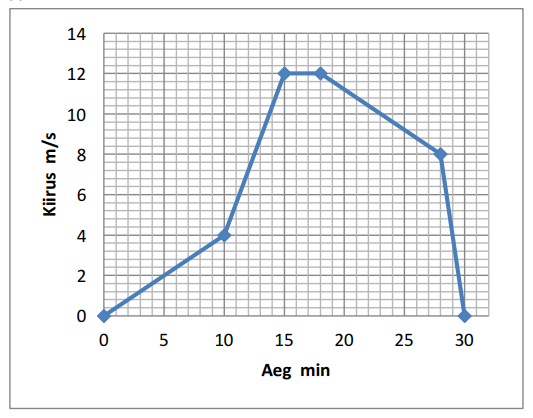
\includegraphics[width=0.5\linewidth]{2018-v2p-01-yl.PNG}
\end{center}
\fi
}


% Ü63
\ylDisplay{Kaks kuulikest} % Ülesande nimi
{EFO žürii} % Autor
{piirkonnavoor} % Voor
{2018} % Aasta
{P 3} % Ülesande nr.
{2} % Raskustase
{
% Teema: Mehaanika
\ifStatement
Kaks kuulikest alustavad samaaegselt võrdsete kiirustega liikumist mööda joonisel näidatud pindu. Kumma kuulikese kiirus on punkti $B$ jõudes suurem või on nende kiirused võrdsed? Kumb kuulike jõuab punkti $B$ varem või jõuavad nad punkti $B$ samaaegselt? Hõõrdejõudu pole vaja arvestada. Põhjendage vastust.
\begin{center}
	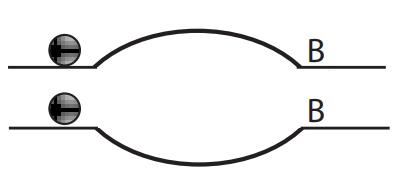
\includegraphics[width=0.5\linewidth]{2018-v2p-03-yl.PNG}
\end{center}
\fi
}


% Ü64
\ylDisplay{Tanker} % Ülesande nimi
{Koit Timpmann} % Autor
{lõppvoor} % Voor
{2018} % Aasta
{P 1} % Ülesande nr.
{2} % Raskustase
{
% Teema: Mehaanika
\ifStatement
Vaiksel merel lähenes sadamale $L = 300$ m pikkune tanker, mis sõitis ühtlase kiirusega $v_1$ sirgjoonelisel kursil. Laevale sõitis vastu samal sihil piirivalve kaater, mis liikus kiirusega $v_2 = 90$ km/h. Kaater sõitis laeva ninast sabani, pööras ümber ja sõitis sama teed tagasi. Kaatril kulus laeva kõrval edasi-tagasi sõitmiseks $t = 25$ s. Kui suure kiirusega $v_1$ sõitis tanker? Ümberpööramiseks kulunud aega ei ole vaja arvestada. 
\fi
}

% Ü65
\ylDisplay{Kaks matkaselli} % Ülesande nimi
{Koit Timpmann} % Autor
{lõppvoor} % Voor
{2018} % Aasta
{P 2} % Ülesande nr.
{2} % Raskustase
{
% Teema: Mehaanika
\ifStatement
Kaks matkaselli pidid jõudma võimalikult kiiresti ja üheaegselt $s = 40$ km kaugusel olevasse laagrisse. Kuna neil oli kahe peale ainult üks äbarik jalgratas, otsustasid nad, et sõidavad jalgrattaga vaheldumisi. Kui kaua „igavles” ratas tee ääres, kui matkasellid jooksid kiirusega $v_1 = 8$ km/h ja sõitsid rattaga kiirusega $v_2 = 15$ km/h?
\fi
}

% Ü66
\ylDisplay{Lennujaam} % Ülesande nimi
{Kristjan Kuppart} % Autor
{piirkonnavoor} % Voor
{2019} % Aasta
{P 4} % Ülesande nr.
{2} % Raskustase
{
% Teema: Mehaanika
\ifStatement
Jüri ja Mari astuvad lennujaama transportlindile, mis liigub kiirusega $u = 0,8$ m/s. Kuna Maril on igav, jookseb ta transportlindi lõppu, pöörab kohapeal ümber ning jookseb mööda linti tagasi Jürini. Kui kaugel transportlindi algusest nad kohtuvad, kui Maril kulus lindi algusest lõppu jooksmiseks $t = 40$ s?
\fi
}


% Ü67
\ylDisplay{Plokid} % Ülesande nimi
{Koit Timpmann} % Autor
{lõppvoor} % Voor
{2019} % Aasta
{P 3} % Ülesande nr.
{2} % Raskustase
{
% Teema: Mehaanika
\ifStatement
Süsteem koosneb ühest liikuvast ja ühest liikumatust plokist ning kahest koormisest massidega $m_1 = 150$ $g$ ja $m_2 = 100$ g (vt joonist). Koormisi hoitakse paigal ning lastakse siis lahti. Kui suur on koormise $m_1$ kiirus hetkel, kui see on läbinud vahemaa $s = 0,5$ m. Plokkide massi ja hõõrdumist süsteemis ei ole tarvis arvestada.
\begin{center}
	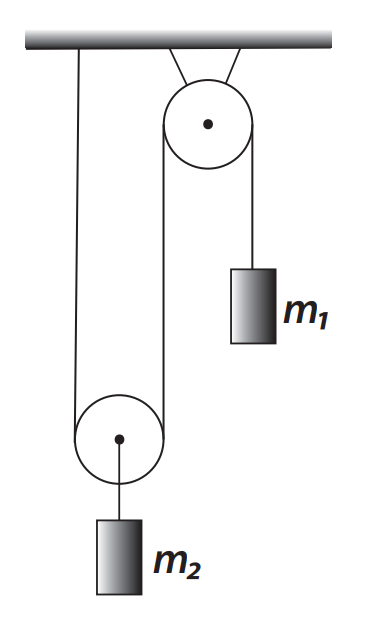
\includegraphics[width=0.5\linewidth]{2019-v3p-03-yl.PNG}
\end{center}
\fi
}

% Ü68
\ylDisplay{Rong} % Ülesande nimi
{Koit Timpmann} % Autor
{lõppvoor} % Voor
{2019} % Aasta
{P 22} % Ülesande nr.
{2} % Raskustase
{
% Teema: Mehaanika
\ifStatement
Paigalseisust liikuma hakanud raske kaubarong suurendab ühtlaselt kiirust. Pärast esimese $1000$ meetri läbimisel on rong saavutanud kiiruse $v = 10,0$ $m/s$. Kui palju suureneb rongi kiirus teisel kilomeetril?
\fi
}

% Ü69
\ylDisplay{Bussid} % Ülesande nimi
{Moorits Mihkel Muru} % Autor
{piirkonnavoor} % Voor
{2020} % Aasta
{P 3} % Ülesande nr.
{2} % Raskustase
{
% Teema: Mehaanika
\ifStatement
Juku sõidab bussiga Tallinnast Berliini ($s = 1558$ km) ja otsustas tee peal ära lugeda mitut Berliin-Tallinn bussi ta näeb vastu tulemas. Kui Berliinist väljuvad Tallinna suunas bussid igal täis- ja pooltunnil (nagu ka Tallinast Berliini) ja busside keskmise kiirused on $v = 85$ km/h, siis mitu bussi Juku kogu tee peale kokku luges?
\fi
}


% Ü70
\ylDisplay{Kanali sild} % Ülesande nimi
{Eero Uustalu} % Autor
{piirkonnavoor} % Voor
{2020} % Aasta
{P 4} % Ülesande nr.
{2} % Raskustase
{
% Teema: Mehaanika
\ifStatement
Laevatatav kanal laiusega $d = 8$ m ja sügavusega $h = 5$ m ristub maanteega kogulaiusega $l = 18$ m ja on viidud maanteest üle sillaga mille miinimumkõrgus maantee pinnast on $k = 7$ m. Sildeava on maantee laiune. Kui suur peaks olema silla kandevõime tonnides, et sellest tohiks üle sõita antud kanalile sobilik laev kogukaaluga $m = 2100$ t? Vee tihedus $\rho = 1000$ $kg/m^3$.
\fi
}

% Ü71
\ylDisplay{Jangtse kiirus} % Ülesande nimi
{EFO žürii} % Autor
{piirkonnavoor} % Voor
{2020} % Aasta
{P 6} % Ülesande nr.
{2} % Raskustase
{
% Teema: Mehaanika
\ifStatement
Pärast seda, kui 2009. aastal valmis Jangtse jõel $2335$ meetri pikkune ja $101$ meetri kõrgune tamm, millega seonduv hüdroelektrijaam on maailma suurim, sai võimalikuks hakata korraldama laevakruiise imelisel Jangtse jõel. Reisikorraldajate väitel läbib laev $650$ km allavoolu kolme ööpäevaga. Ülesvoolu sõites kulub sama vahemaa läbimiseks neli ööpäeva. Kui suur on keskmine voolukiirus ülespaisutatud Jangtse jões?
\fi
}

% Ü72
\ylDisplay{Kohtumispaik} % Ülesande nimi
{EFO žürii} % Autor
{lõppvoor} % Voor
{2020} % Aasta
{P 2} % Ülesande nr.
{2} % Raskustase
{
% Teema: Mehaanika
\ifStatement
Kahe linna vaheline kaugus $s = 180$ km. Linnast $A$ väljub auto linna $B$ suunas. Auto keskmine kiirus terve teekonna ulatuses $v_1 = 75$ km/h. Auto jõuab linna $B$ ning $1,5$ tunni möödudes väljub linnast $B$ tagasi linna $A$ suunas. Ka tagasiteel on auto keskmine kiirus $75$ km/h. Pool tundi pärast esimese auto väljumist linnast $A$ väljub linnast $B$ teine auto linna $A$ suunas. See auto liigub terve tee keskmise kiirusega $v_2 = 80$ km/h. Viibinud $2$ tundi linnas $A$ suundub teine auto tagasi koju liikudes jälle keskmise kiirusega $v_2 = 80$ $km/h$. Kui kaugel linnast $A$ autod kohtuvad autod tagasiteel? 
\fi
}


% Ü73
\ylDisplay{Plokid} % Ülesande nimi
{Tundmatu autor} % Autor
{lõppvoor} % Voor
{2012} % Aasta
{P 7} % Ülesande nr.
{3} % Raskustase
{
% Teema: Mehaanika
\ifStatement
Liikuva ploki abil on võimalik saavutada jõus kahekordne võit (vt joonis). Joonistage sellised plokkide süsteemid, mille kasutamisel koorma tõstmiseks on jõu võit: a) $5$-kordne; b) $2,5$-kordne.
\begin{center}
	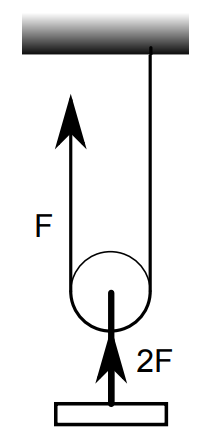
\includegraphics[width=0.5\linewidth]{2012-v3p-07-yl.PNG}
\end{center}
\fi
}

% Ü74
\ylDisplay{Litter} % Ülesande nimi
{Tundmatu autor} % Autor
{lõppvoor} % Voor
{2012} % Aasta
{P 9} % Ülesande nr.
{3} % Raskustase
{
% Teema: Mehaanika
\ifStatement
Joonisel on kujutis, mille jättis pealtvaates pika säriajaga tehtud fotole lambike, mis oli kinnitatud jääl hõõrdevabalt libisevale ja pöörlevale kettakujulisele litrile. Lambi kinnituskoht asub $a = 4,5$ cm kaugusel litri püstteljest. Lamp põleb tuhmilt siniselt, kuid vilgatab  iga $t = 0,10$ s järel heledamalt punaselt. Fotole on lisatud tundmatu sammuvahega ruudustik. Leidke litri edasiliikumiskiirus.
\begin{center}
	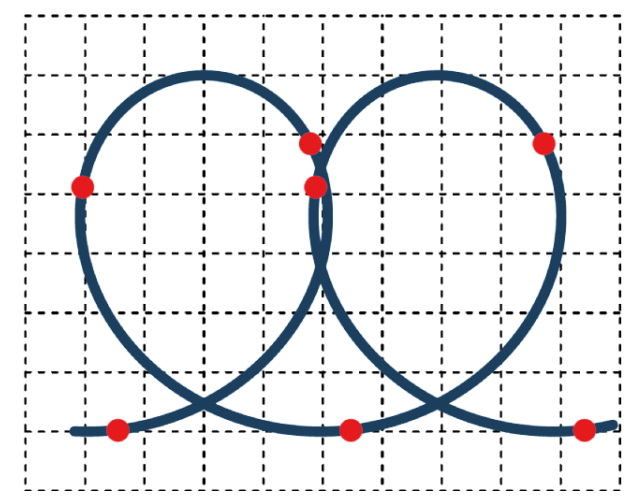
\includegraphics[width=0.5\linewidth]{2012-v3p-09-yl.PNG}
\end{center}
\fi
}


% Ü75
\ylDisplay{Uppuv klots} % Ülesande nimi
{Tundmatu autor} % Autor
{lõppvoor} % Voor
{2012} % Aasta
{P 10} % Ülesande nr.
{3} % Raskustase
{
% Teema: Mehaanika
\ifStatement
Vees ujub vahtrapuust kuup servapikkusega $a = 10$ cm tihedusega $\rho_{vaher} = 700$ $kg/m^3$ . Kuubi sees on silindriline õõnsus läbimõõduga $b = 4,5$ cm (vt. joonist). Õõnsus on alt suletud õhukese korgiga. 
a) Arvutage, kas kuup upub, kui õõnsus täita liivaga? Liiva tihedus on $\rho_{liiv} = 2700$ $kg/m_3$ ja vee tihedus on $\rho_{vesi} = 1000$ $kg/m^3$. 
b) Kui korgile mõjuv summaarne jõud on suurem kui $1,8$ N, läheb kork katki. 
Mis on maksimaalne liiva kõrgus, mida saab õõnsusesse valada?
\begin{center}
	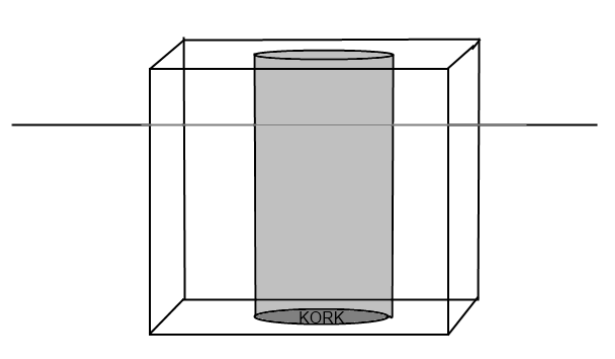
\includegraphics[width=0.5\linewidth]{2012-v3p-10-yl.PNG}
\end{center}
\fi
}

% Ü76
\ylDisplay{Vihm} % Ülesande nimi
{Tundmatu autor} % Autor
{piirkonnavoor} % Voor
{2013} % Aasta
{P 10} % Ülesande nr.
{3} % Raskustase
{
% Teema: Mehaanika
\ifStatement
Tuulevaikse ilmaga vihma käes seisev inimene saab märjaks $t = 2$ minutiga. Kui inimene jookseb kiirusega $v_2 = 18$ km/h, saab ta märjaks $t_2 = 0,5$ minutiga. Kui kiiresti saab inimene märjaks siis, kui kõnnib kiirusega $v_1 = 6$ km/h? Eeldage, et inimese keha on samas asendis seismisel, jooksmisel ja kõndimisel ning et inimest võib lähendada risttahukaga. Märjaks saamine tähendab seda, et inimesele langeb teatud kindel kogus vett.
\fi
}

% Ü77
\ylDisplay{Klapp} % Ülesande nimi
{Tundmatu autor} % Autor
{lõppvoor} % Voor
{2013} % Aasta
{P 8} % Ülesande nr.
{3} % Raskustase
{
% Teema: Mehaanika
\ifStatement
Vett täis anumas asub vertikaalselt õhukeste seintega toru, mille sisemine läbimõõt on $d = 2$ cm. Toru alumine ots on $70$ cm sügavusel vees ja selle vastu on surutud tihedalt õhukene ruudukujuline plaat küljepikkusega $a = 3$ cm. Plaadi pindtihedus (massi ja pindala suhe) $\sigma  = 4,5$ $kg/m^2$ . Torusse valatakse õli tihedusega $rho_õ = 900$ $kg/m^3$ . Kui kõrge õlisamba võib torusse valada, enne kui plaat eraldub toru otsast? Plaadi ja toru paksust ei ole vaja arvestada. Vee tihedus $\rho_v = 1000$ $kg/m^3$. 
\fi
}

% Ü78
\ylDisplay{Paadid} % Ülesande nimi
{Tundmatu autor} % Autor
{lõppvoor} % Voor
{2013} % Aasta
{P 10} % Ülesande nr.
{3} % Raskustase
{
% Teema: Mehaanika
\ifStatement
 Laial jõel sõidavad kaks paati, mõlema kiirused ja kiiruste suunad on konstantsed. Veevoolu kiirus on jões samuti kõikjal üks ja sama ning paralleelne kallastega. Juuresolev foto on tehtud õhust, otse ülevalt alla; paatide asukohad on tähistatud ruudu ja kolmnurgaga, paatidelt vette kukkunud praht aga tähekestega. Üks paat alustas teekonda punktist $A$; on teada, et paadid kohtusid. Milisest jõekalda punktist alustas teekonda teine paat? Lahendus leidke geomeetrilise konstrueerimise teel lisalehel.
\begin{center}
	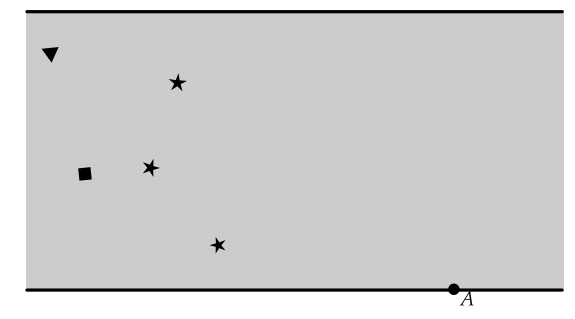
\includegraphics[width=0.5\linewidth]{2013-v3p-10-yl.PNG}
\end{center}
\fi
}


% Ü79
\ylDisplay{Lennukid} % Ülesande nimi
{Tundmatu autor} % Autor
{piirkonnavoor} % Voor
{2014} % Aasta
{P 9} % Ülesande nr.
{3} % Raskustase
{
% Teema: Mehaanika
\ifStatement
Kaks lennukit lendavad samal kõrgusel kiirustega $v_1 = 800$ $km/h$ ja $v_2 = 600$ $km/h$. Vaadeldaval hetkel on lennukite liikumise sihid omavahel risti ning kumbki lennuk paikeb sihtide ristumispunktist kaugusel $a = 20$ $km$. Leidke, milline on lennukite vähim vahekaugus järgneva liikumise jooksul, kui eeldada, et kumbki lennuk kurssi ei muuda.\fi
}

% Ü80
\ylDisplay{Äpardus plokiga} % Ülesande nimi
{Tundmatu autor} % Autor
{lõppvoor} % Voor
{2014} % Aasta
{P 10} % Ülesande nr.
{3} % Raskustase
{
% Teema: Mehaanika
\ifStatement
\begin{center}
	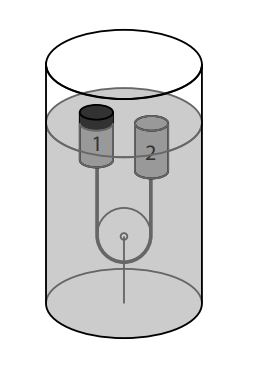
\includegraphics[width=0.5\linewidth]{2014-v3p-10-yl.PNG}
\end{center}
Silindrilises anumas põhjapindalaga $S$ on vesi tihedusega $\rho$. Anuma põhjas on plokk ja üle hõõrdevabalt pöörleva plokiratta on tõmmatud nöör. Nööri otste külge on kinnitatud kaks veest väiksema tihedusega keha. Plokk takistab nende kehade veepinnale kerkimist (vt joonis). Kummagi keha ruumala on $V$ . Ühe keha tihedus on $\rho 1$ ja teise keha tihedus $ \rho 2$, kusjuures $\rho1 < \rho2 < \rho$. Plokinöör on nii pikk, et kumbki kehadest ei puuduta plokki ning nii lühike, et üks keha on tõmmatud üleni vee alla. Kui palju muutub anumas oleva vee tase kui plokinöör katkeb ja mõlemad kehad kerkivad vee pinnale?
\fi
}

% Ü81
\ylDisplay{Kuup vedelikes} % Ülesande nimi
{Tundmatu autor} % Autor
{lõppvoor} % Voor
{2015} % Aasta
{P 4} % Ülesande nr.
{3} % Raskustase
{
% Teema: Mehaanika
\ifStatement
Anum on täidetud kahe mitteseguneva vedelikuga tihedustega $\rho_1$ ja $\rho_2$. Vedelikku lastakse kuup külje pikkusega $l$. Kui sügavale $x$ vajub kuup teise vedelikku, kui kuubi tihedus on $\rho$? On teada, et $\rho_1 < \rho < \rho_2$.
\fi
}

% Ü82
\ylDisplay{Varras} % Ülesande nimi
{Tundmatu autor} % Autor
{lõppvoor} % Voor
{2015} % Aasta
{P 5} % Ülesande nr.
{3} % Raskustase
{
% Teema: Mehaanika
\ifStatement
Varras $AC$ võib pöörelda ümber punkti $B$ ja varras $DF$ ümber punkti $F$. Varda $AC$ otsad on niitidega kinnitatud varda $DF$ külge. On teada, et$ AB = 2a$,$ BC = a$ ja $DF = 4a$. Kui suured on niitides $AD$ ja $CE$ mõjuvad jõud? Varda $DF$ mass $m = 6$ $kg$ ning on jaotunud ühtlaselt üle kogu varda. Varda $AC$ massi ei ole tarvis arvestada.
\begin{center}
	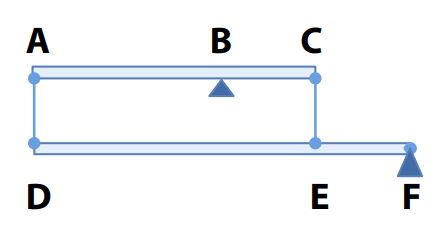
\includegraphics[width=0.5\linewidth]{2015-v3p-05-yl.PNG}
\end{center}
\fi
}

% Ü83
\ylDisplay{Liiklejad} % Ülesande nimi
{Tundmatu autor} % Autor
{lõppvoor} % Voor
{2015} % Aasta
{P 10} % Ülesande nr.
{3} % Raskustase
{
% Teema: Mehaanika
\ifStatement
 Sirgel teel sörgib Ants kiirusega $v_A = 7,0$ km/h. Samal teel sõidab Birgit mopeediga samas suunas kiirusega $v_B = 25$ km/h. Teist sellega lõikuvat sirget teed mööda sõidab jalgrattaga Gerd kiirusega $v_G = 20$ km/h. Vahemaa Antsu ja Gerdi vahel jääb kogu aeg võrdseks vahemaaga Gerdi ja Birgiti vahel. Leidke Gerdi kiirus Birgiti suhtes.
\fi
}

% Ü84
\ylDisplay{Kera vees} % Ülesande nimi
{Tundmatu autor} % Autor
{piirkonnavoor} % Voor
{2016} % Aasta
{P 6} % Ülesande nr.
{3} % Raskustase
{
% Teema: Mehaanika
\ifStatement
Anuma põhjast lahti lastud õõnsusega kera massiga $m$ ja raadiusega $R$ tõusis ühtlase kiirusega vedeliku pinnale. Kui suur lisamass tuleks paigutada kera õõnsusesse, et see vajuks vedelikus põhja sama kiirusega kui enne tõusis. Vedelikus kerale mõjuv takistusjõud on võrdeline kera kiirusega. Vedeliku tihedus on  ja kera ruumala valem $V = \frac{4}{4} \cdot \pi \cdot R3$.
\fi
}

% Ü85
\ylDisplay{Paat vees} % Ülesande nimi
{Tundmatu autor} % Autor
{piirkonnavoor} % Voor
{2016} % Aasta
{P 9} % Ülesande nr.
{3} % Raskustase
{
% Teema: Mehaanika
\ifStatement
Mootorpaat sõidab jõe ääres asuvast külast $A$ ülesvoolu $s = 10$ km kaugusel olevasse teise külasse $B$. Ülesvoolu sõites kulub tal külla $B$ jõudmiseks $t_1 = 4$ h. Allavoolu tagasi sõites saab paadil $t_k = 24$ min pärast kütus otsa ning edasi kulgeb ta jõevoolu kiirusel. Küladevahelise maa läbimiseks kulub paadil tagasi tulles $t_2 = 2$ h. Kui kaugel oli paat külast $A$, kui tal kütus otsa sai?
\fi
}

% Ü86
\ylDisplay{Kütusekulu linnas} % Ülesande nimi
{Tundmatu autor} % Autor
{piirkonnavoor} % Voor
{2016} % Aasta
{P 10} % Ülesande nr.
{3} % Raskustase
{
% Teema: Mehaanika
\ifStatement
Oletame lihtsustavalt, et sõiduauto massiga $m = 1500$ kg peab linnaliikluses valgusfooride, sebrade jms tõttu peatuma iga vahemaa $L = 500$ m tagant. Peatumiste vahel sõidab auto kiirusega $v = 50$ $km/h$. Arvutage välja linnaliikluses sagedastest peatumistest tingitud auto keskmine kütusekulu (liitrit sajale kilomeetrile). Arvestage, et bensiini tihedus $\rho = 0,72$ $kg/dm^3$ ning kütteväärtus $M = 44$ MJ/kg, millest mootor muundab $\eta = 25$\% kasulikuks tööks. Õhutakistusega liikumisel ega kütusekuluga seismisel ärge arvestage. Märkus: Kineetilise energia valem $E_k = \frac{mv^2}{2}$ .\fi
}

% Ü87
\ylDisplay{Glütseriin torus} % Ülesande nimi
{Autor} % Autor
{lõppvoor} % Voor
{2016} % Aasta
{P 7} % Ülesande nr.
{3} % Raskustase
{
% Teema: Mehaanika
\ifStatement
Purki, milles on vesi, on paigutatud vertikaalne lihvitud otstega toru, mida hoitakse kinni. Toru alumise otsa vastas on sileda pinnaga teeküünal. Teeküünla läbimõõt $D = 3,5$ cm, toru läbimõõt $d = 1,5$ cm. Teeküünla kõrgus $h_k = 1,2$ cm ja küünla tihedus $\rho_k = 0,9$ $g/cm^3$ . Torusse on valatud $h = 5$ cm kõrgune sammas glütseriini, mille tihedus on $\rho_g = 1,26$ $g/cm^3$ . Kui sügaval veepinnast $H$ peab olema toru alumine ots, et glütseriin sellest vette ei voolaks? Vee tihedus on $\rho_v = 1,0$ $g/cm^3$.
\fi
}

% Ü88
\ylDisplay{Pidurdus} % Ülesande nimi
{Autor} % Autor
{lõppvoor} % Voor
{2016} % Aasta
{P 8} % Ülesande nr.
{3} % Raskustase
{
% Teema: Mehaanika
\ifStatement
Auto sõidab teel, mille kõrguse muut teepikkuse kohta $k = $ $1/30$ . Ühesuguse algkiiruse ning pidurdusjõu korral jääb auto ülesmäge liikudes seisma $s_1 = 25$ m, allamäge liikudes aga $s_2 = 30$ m jooksul. Mis on auto algkiiruse $v$ väärtus?
\fi
}

% Ü89
\ylDisplay{Kalapüük} % Ülesande nimi
{EFO žürii} % Autor
{piirkonnavoor} % Voor
{2017} % Aasta
{P 7} % Ülesande nr.
{3} % Raskustase
{
% Teema: Mehaanika
\ifStatement
Jaak ja Jüri elavad külas jõe kaldal ning armastavad kalal käia. Ühel päeval nad otsustasid, et üks neist sõidab kalastama allavoolu, teine ülesvoolu. Nad leppisid kokku, et sõidavad paadiga täpselt pool tundi ning hakkavad siis õngitsema. Õngitsemise ajal triivivad paadid veevooluga kaasa. Jaak sõitis ülesvoolu, tema paadi mootor arendas seisvas vees kiirust $24$ km/h. Jüri sõitis allavoolu. Tema paadi mootor arendas seisvas vees kiirust $20$ km/h. Jõe voolukiirus on $2$ km/h. Pärast tunniajast õngitsemist hakkas Jüri kalastuskohas vihma sadama. Ta helistas kohe Jaagule ja teatas, et hakkab koju sõitma. Jaak tahtis küla sadamasillale jõuda samaaegselt Jüriga ja arvutas, et võib veel veidi kala püüda, enne kui sõitma hakkab. Kui kaua võis Jaak veel kala püüda, et jõuda külasse samaaegselt Jüriga?
\fi
}

% Ü90
\ylDisplay{Drooni vari} % Ülesande nimi
{Autor} % Autor
{lõppvoor} % Voor
{2017} % Aasta
{P 10} % Ülesande nr.
{3} % Raskustase
{
% Teema: Mehaanika
\ifStatement
Õhtusel ajal seisab Juku tenniseväljaku ääres, mille laius on $a $ning vaatleb, kuidas tema sõber lennutab drooni. On teada, et drooni kiiruse horisontaalkomponent on kogu lennu vältel $v$ ning horisontaalkomponendi suund ei muutu. Samuti on teada, et Päike asub otse drooni taga ja päikesekiired langevad maapinnale maapinna suhtes nurga $\alpha$ all. Algul lendab droon ühtlase kiirusega $v$ paralleelselt maapinnaga. Drooni vari ületab tenniseväljaku ajaga $t_1$. Droon jätkab lendamist sirgjoonelisel trajektooril, kuid mitte enam paralleelselt maapinnaga. Drooni vari liigub uuesti üle tenniseväljaku, nüüd eelnevaga vastassuunas. Teisel juhul ületab vari tenniseväljaku ajaga $t_2$. Kui palju muutus drooni lennukõrgus $h$ ajavahemiku $t_2$ jooksul?
\fi
}

% Ü91
\ylDisplay{Kontraktsioon} % Ülesande nimi
{EFO žürii} % Autor
{piirkonnavoor} % Voor
{2018} % Aasta
{P 5} % Ülesande nr.
{3} % Raskustase
{
% Teema: Mehaanika
\ifStatement
Omavahel segatakse vett ja piiritust nii, et tekkinud lahuse ruumala $V = 1 dm^3$ ning lahuses on massi järgi $p = 44,1\%$ piiritust. Leidke tekkinud lahuse tihedus $rho$? Arvestage, et lahuste kokkuvalamisel esineb $\gamma = 6 \%$-line kontraktsioon – saadud lahuse ruumala on $6 \%$ väiksem kui vee ja piirituse ruumalade summa enne kokku valamist. Vee tihedus $\rho_v = 1000$ $kg/m^3$ ning piirituse tihedus $\rho_p = 790$ $kg/m^3$.
\fi
}

% Ü92
\ylDisplay{Kuup vedelikes} % Ülesande nimi
{Koit Timpmann} % Autor
{lõppvoor} % Voor
{2018} % Aasta
{P 4} % Ülesande nr.
{3} % Raskustase
{
% Teema: Mehaanika
\ifStatement
Anumas on kaks mittesegunevat vedelikku, milles heljub tahkest ainest kuup küljepikkusega $l = 10$ $cm$. Ühe vedeliku tihedus on $\rho_1 = 0,8$ $g/cm^3$, teise vedeliku tihedus $\rho_2 = 1,2$ $g/cm^3$ ja kuubi aine tihedus $\rho_k = 1,1$ $g/cm^3$ . Ülemise vedelikukihi paksus on suurem kuubi külje pikkusest. Kui sügaval alumises vedelikus asetseb kuup?
\fi
}


% Ü93
\ylDisplay{Veejuga} % Ülesande nimi
{Jonatan Kalmus} % Autor
{lõppvoor} % Voor
{2018} % Aasta
{P 8} % Ülesande nr.
{3} % Raskustase
{
% Teema: Mehaanika
\ifStatement
Vertikaalsest kraanist voolab vesi välja algkiirusega $v_0$. Leidke, millisel kaugusel $h$ kraanist on veejoa läbimõõt poole väiksem kui kraanist väljudes. Raskuskiirendus on $g$.
\fi
}

% Ü94
\ylDisplay{Keha vees} % Ülesande nimi
{Koit Timpmann} % Autor
{lõppvoor} % Voor
{2019} % Aasta
{P 6} % Ülesande nr.
{3} % Raskustase
{
% Teema: Mehaanika
\ifStatement
Õpetaja näitas tunnis katset. Kangkaalu ühes kaalukausis oli klaas veega, teises kaalukausis statiiv, mille varda küljes rippus alumiiniumist keha. Kaal oli tasakaalus. Nüüd lasi õpetaja statiivivarda koos selle otsas rippuva kehaga alla, nii et keha sukeldus üleni klaasis olevasse vette. Kui suure massiga lisakoormis tuleb ühele kaalukausile asetada, et kaal oleks uuesti tasakaalus? Kummale? Rippuva keha mass $m = 135$ g. Alumiiniumi tihedus $\rho Al = 2700$ $kg/m^3$ , vee tihedus $\rho_v = 1000$ $kg/m^3$.
\begin{center}
	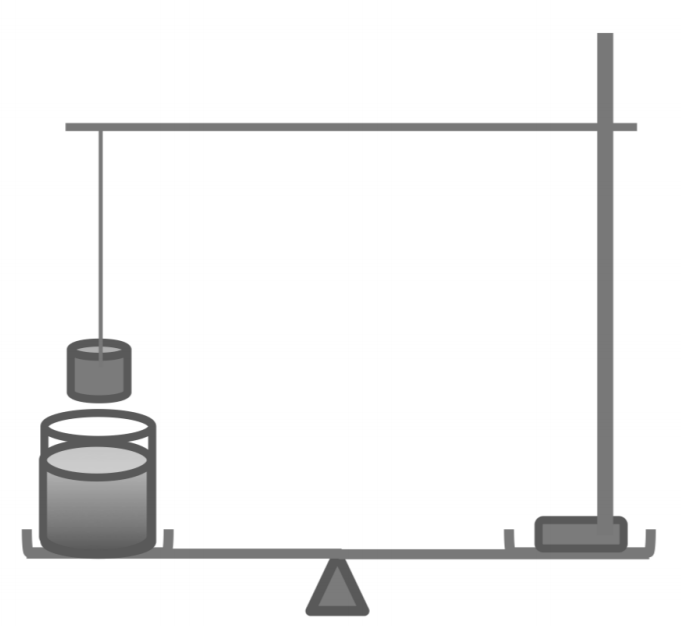
\includegraphics[width=0.5\linewidth]{2019-v3p-06-yl.PNG}
\end{center}
\fi
}

% Ü95
\ylDisplay{Keha vees} % Ülesande nimi
{Jonatan Kalmus} % Autor
{lõppvoor} % Voor
{2019} % Aasta
{P 8} % Ülesande nr.
{3} % Raskustase
{
% Teema: Mehaanika
\ifStatement
Joonisel on lennuki algne asukoht märgitud ristiga. Iga tunni järel mõõdeti lennuki kaugust fikseeritud punktist. Saadud kaugused on joonisel märgitud ringjoonena mõõtepunkti ümber. Konstrueerida kõik võimalikud lennuki trajektoorid $7$ h jooksul, kui on teada, et pärast starti lendas lennuk $4$ h otse, muutis seejärel suunda ning lendas ülejäänud aja samuti otse. Eeldada, et lennuki kiirus maapinna suhtes oli ühtlaselt $500$ km/h. Lahendus esitage lisalehel. NB! Suuna muutus võis olla ka väga väike.
\begin{center}
	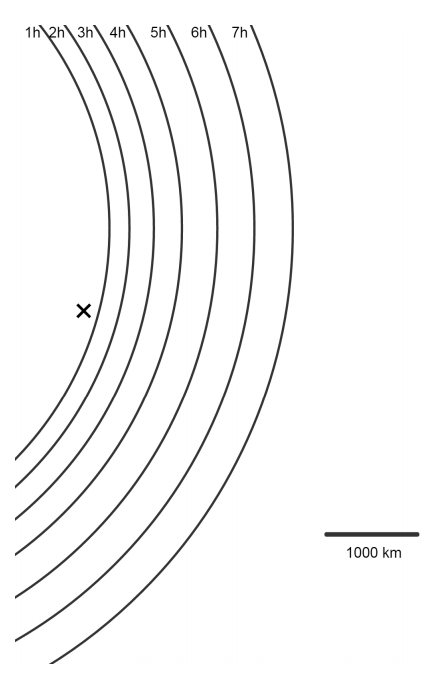
\includegraphics[width=0.5\linewidth]{2019-v3p-08-yl.PNG}
\end{center}
\fi
}
 


% Ü96
\ylDisplay{Ühendatud anumad} % Ülesande nimi
{Kristjan Kuppart} % Autor
{lõppvoor} % Voor
{2019} % Aasta
{P 10} % Ülesande nr.
{3} % Raskustase
{
% Teema: Mehaanika
\ifStatement
Pooleldi veega täidetud omavahel ühendatud anumate ühte harusse valatakse $h = 4$ $cm$ õli. Seejärel asetatakse sinna harusse ujuma ühtlase ristlõikepindalaga puidust klots kõrgusega $L = 10$ $cm$ ja tihedusega $\rho k = 0,5$ $g/cm^3$ . Kui palju tõuseb veetase teises harus võrreldes algse olukorraga, kui klotsi ja haru pindalade suhe $S_h / S_k = 2$? Õli tihedus $\rho_õ = 0,9$ $g/cm^3$ ja vee tihedus $\rho_v = 1$ $g/cm^3$ . Harude ristlõikepindalad on võrdsed ning õli ühest harust teise ei voola.
\fi
}
\newpage\subsection{\protect\StrSubstitute{Soojusõpetus}{-}{ }}

% Ü97
\ylDisplay{Palli soojenemine} % Ülesande nimi
{Tundmatu autor} % Autor
{piirkonnavoor} % Voor
{2013} % Aasta
{P 2} % Ülesande nr.
{1} % Raskustase
{
% Teema: Soojusõpetus
\ifStatement
Kui palju soojeneb $100$ grammine kummist pall (erisoojusega $c = 1400 J/kg^{\circ}C$), mis kukub lauale $4$ meetri kõrguselt ning põrkab tagasi $230$ $cm$ kõrgusele? Eeldada, et pall saab $90\%$ soojushulgast.
\fi
}

% Ü98
\ylDisplay{Lumi} % Ülesande nimi
{Tundmatu autor} % Autor
{piirkonnavoor} % Voor
{2014} % Aasta
{P 6} % Ülesande nr.
{1} % Raskustase
{
% Teema: Soojusõpetus
\ifStatement
Juku otsustas välja uurida, mis temperatuuril $t_l$ on lumi õues kõrguvate hangede sisemuses. Tal endal termomeetrit ei olnud, aga ta teadis, et tema maja ventilatsioonisüsteem hoiab sisetemperatuuri $t_s = 20 ^{\circ} C$ . Esimese asjana lasi ta öö läbi seista kausitäiel veel, et see oleks toatemperatuuril. Järgmisel päeval tõi ta hange sisemusest termosetäie lund ja jagas selle kahte võrdsesse osasse. Ühele osale tilgutas ta peale toatemperatuuril hoitud vett, kuni kogu lumi oli sulanud. Vett kulus selleks $V_1 = 880$ ml. Teise osa sulatas ta ära ja mõõtis saadud vee ruumalaks $V_2 = 210$ ml. Lõpuks otsis ta Wikipediast välja, et vee erisoojus on $c_v = 4180 J/kg^{\circ}C$, jää erisoojus $c_l = 2110 J/kg^{\circ}C$ ja jää sulamissoojus $\lambda = 334$ kJ/kg. Mis temperatuuril $t_l$ oli lumi?
\fi
}

% Ü99
\ylDisplay{Vihm} % Ülesande nimi
{EFO žürii} % Autor
{piirkonnavoor} % Voor
{2018} % Aasta
{P 8} % Ülesande nr.
{1} % Raskustase
{
% Teema: Soojusõpetus
\ifStatement
Kui paksu lumekihi sulataks ära $t = 5$ h jooksul pidevalt sadav vihm temperatuuriga $T = 5$ $^{\circ}$C, kui vihmavee kogunemise kiirus $h = 12$ mm/h? Lume kohevus on selline, et $1$ $cm$ paksune lumekiht annab sulades $1,2$ mm paksuse veekihi. Vee erisoojus $c = 4200 \frac{J}{kg \cdot ^{\circ}}C$, jää sulamissoojus $\lambda = 340$ kJ/kg, vee tihedus $\rho = 1000$ $kg/m^3$ .
\fi
}

% Ü100
\ylDisplay{Külmkapp} % Ülesande nimi
{EFO žürii} % Autor
{piirkonnavoor} % Voor
{2019} % Aasta
{P 2} % Ülesande nr.
{1} % Raskustase
{
% Teema: Soojusõpetus
\ifStatement
Juku tahtis valmistada jäävett ning asetas $V_0 = 1$ $dm^3$ kaevust võetud $t_v = 4^{\circ}$C) vett pudeliga sügavkülma. Nelja tunni pärast võttis Juku külmkapist välja ning kallas vee kannu. Kannus oli $V_1 = 0.5$ $dm^3$ vett. Milline on külmkapi sügavkülma külmutusvõimsus $N$? Jää sulamissoojus $\lambda 340$ kJ/kg, vee erisoojus $c = 4200 \frac{J}{kg \cdot ^{\circ}C}$, vee tihedus $\rho = 1000$ $kg/m^3$.
\fi
}

% Ü101
\ylDisplay{Mahl ja jää} % Ülesande nimi
{Erkki Tempel} % Autor
{lõppvoor} % Voor
{2019} % Aasta
{P 1} % Ülesande nr.
{1} % Raskustase
{
% Teema: Soojusõpetus
\ifStatement
Jukul oli $m_m = 500$ g toatemperatuuril $(t_m = 20^{\circ}$C) olevat mahla. Mahla jahutamiseks lisas ta sinna sisse $m_j = 100$ g jääd temperatuuril $t_j = -18^{\circ}$C. Milline oli mahla temperatuur pärast soojustasakaalu saavutamist? Soojuskadudega väliskeskkonda ei ole vaja arvestada. Mahla erisoojus $c_m = 4200 J/(kg \cdot ^{\circ}C)$, jää erisoojus $c_j = 2100 J/(kg \cdot ^{\circ}C)$ ning jää sulamissoojus $\lambda = 330$ kJ/kg.
\fi
}

% Ü102
\ylDisplay{Glütseriin} % Ülesande nimi
{Tundmatu autor} % Autor
{piirkonnavoor} % Voor
{2010} % Aasta
{P 7} % Ülesande nr.
{2} % Raskustase
{
% Teema: Soojusõpetus
\ifStatement
Paksude seintega anum on pilgeni täidetud glütseriiniga ning tihedalt suletud, kuid anuma seinas on tilluke ava ristlõikepindalaga $s = 0,1$ $mm^2$ . Anumas, glütseriini sees on elektrispiraal, mida kuumutatakse võimsusega $P = 1$ kW. Glütseriini ruumpaisumistegur on $\alpha = 5,1 \cdot 10^{-4} \frac{1}{C}$, tihedus $\rho = 1260 kg/m^3$ ja erisoojus $c = 2350 J/(kg \cdot C)$. Millise kiirusega $v$ väljub glütseriinijuga tillukesest avast? Glütseriini kokkusurutavus ning anuma seinte paisumine lugeda tühiselt väikeseks. Märkus: ruumpaisumistegur kirjeldab ruumala suhtelist suurenemist temperatuuri tõusmisel 1 C võrra.
\fi
}

% Ü103
\ylDisplay{Radiaatorid} % Ülesande nimi
{Tundmatu autor} % Autor
{piirkonnavoor} % Voor
{2011} % Aasta
{P 8} % Ülesande nr.
{2} % Raskustase
{
% Teema: Soojusõpetus
\ifStatement
Kahte radiaatorit läbib ajauhikus võrdne hulk vett. Esimesse radiaatorisse siseneb vesi temperatuuriga $t_{1s} = 45^{\circ}$C ja väljub temperatuuriga $t_{1v} = 35^{\circ}$C. Teise radiaatorisse siseneb vesi temperatuuriga $t_{2s} = 40^{\circ}$C ja väljub temperatuuriga $t_{2v} = 25^{\circ}$C. Kumma radiaatori küttevõimsus on suurem ja mitu korda?
\fi
}

% Ü104
\ylDisplay{Bensiinikulu} % Ülesande nimi
{Tundmatu autor} % Autor
{piirkonnavoor} % Voor
{2012} % Aasta
{P 4} % Ülesande nr.
{2} % Raskustase
{
% Teema: Soojusõpetus
\ifStatement
Leidke kiirusel $v = 90$ km/h sõitva auto bensiinikulu liitrites $s = 100$ km kohta, kui mootoris kütuse põlemisel eralduv  võimsus on sellel kiirusel $P = 58$ kW. Bensiini põlemisel eralduv soojushulk ruumalaühiku kohta on $\rho = 35$ MJ/l.
\fi
}

% Ü105
\ylDisplay{Külmunud tort} % Ülesande nimi
{Tundmatu autor} % Autor
{lõppvoor} % Voor
{2012} % Aasta
{P 3} % Ülesande nr.
{2} % Raskustase
{
% Teema: Soojusõpetus
\ifStatement
Juss vedas talvel majast sauna läbimõõduga $D = 1,2$ cm ja pikkusega $l = 10$ m veetoru. Veetoru lahtisulatamiseks oli ta selle sisse paigutanud vasktraadi läbimõõduga $d = 1,0$ mm. Jää sulatamiseks läheb $60\%$ traadis eralduvast soojusest. Õues on õhutemperatuur $T = -10^{\circ}$C. Kui palju aega kulub kogu veetorus oleva jää sulatamiseks, kui traadi otstele rakendada pinge $U = 12$ V? Jää tihedus on $\rho_j = 920 $ $kg/m^3$ , jää erisoojus on $c_j = 2100$ $\frac{J}{kg \cdot ^{\circ} C}$, jää sulamissoojus $\lambda_j = 340$ $\frac{kJ}{kg}$, vase eritakistus $\rho_{Cu} = 0,017$ $\frac{\Omega \cdot mm^2}{m}$.
\fi
}

% Ü106
\ylDisplay{Hõõrdkeevitus} % Ülesande nimi
{Tundamtu autor} % Autor
{lõppvoor} % Voor
{2012} % Aasta
{P 5} % Ülesande nr.
{2} % Raskustase
{
% Teema: Soojusõpetus
\ifStatement
Suhteliselt uus keevitustehnoloogia on hõõrdkeevitus. See seisneb selles, et üks liidetavatest detailidest pannakse pöörlema ning surutakse vastu teist. Kui tekkinud soojus on detailid peaaegu sulamistemperatuurini kuumutanud, jätakse pöörlev toru seisma ning suure rõhu all moodustub side. Vaatame olukorda, kus kaks vasest torujuppi tahetakse kokku keevitada. Leidke, kui suur hõõrdejõud peab pöörlemisel rakenduma, et tekiks piisavalt suur soojushulk $\triangle t = 6,0$ s jooksul. Toru pöörlemiskiirus on $f = 1200$ pööret minutis. Lihtsustatult võib eeldada, et mõlema toru otsast kuumeneb ühtlaselt $l = 0,50$ cm pikkune jupp. Torude diameeter on $D = 8,0$ cm, seina paksus $d = 5,0$ mm. Torud on alguses teoatemperatuuril $T_0 = 20^{\circ}$C. Liitumine toimub temperatuuril $T_1 = 810^{\circ}C$. Vase tihedus on $\rho = \SI{8.9}{g.cm^3}$ ning erisoojus $c = 390$ $\frac{J}{kg \cdot K}$. Soojuskadudega ümbritsevasse keskkonda mitte arvestada. 
\fi
}

% Ü107
\ylDisplay{Veepudel} % Ülesande nimi
{Tundmatu autor} % Autor
{piirkonnavoor} % Voor
{2013} % Aasta
{P 4} % Ülesande nr.
{2} % Raskustase
{
% Teema: Soojusõpetus
\ifStatement
Külma ilmaga oli autosse ununenud $1,5$ liitrine täis veepudel. Auto juurde tulnud autojuht Koit ei uskunud oma silmi: temperatuur autos oli $-5 ^{\circ}$ C, aga vesi pudelis ei olnud kulmunud. Koidule tuli meelde, et ta oli kunagi kuulnud, et väga puhas vedelik võib olla vedelas olekus ka allpool tahkumistemperatuuri. Selle kontrollimiseks võttis ta pudeli ja raputas seda ning suhteliselt kiiresti muutus selles osa veest jääks. Mitu grammi jääd tekkis pudelisse? Vee erisoojus $c = 4200 J/kg^{\circ}C$ ja tihedus on $\rho = 1000 kg/m^3$, jää sulamissoojus $\lambda = 340$ kJ/kg.
\fi
}

% Ü108
\ylDisplay{Litter} % Ülesande nimi
{Tundmatu autor} % Autor
{lõppvoor} % Voor
{2013} % Aasta
{P 4} % Ülesande nr.
{2} % Raskustase
{
% Teema: Soojusõpetus
\ifStatement
Metallist litter raadiusega $r$ ja algpaksusega $h$ libiseb kahe suure heast soojusisolaatorist plaadi vahel. Plaadid on maapinna suhtes täpselt nii kaldu, et litter libiseks ühtlase kiirusega, ja plaatide vahekaugus on $l$, mis on väga vähe erinev litri paksusest. Kui pika maa saab litter vertikaalsuunas läbida enne kinnijäämist? Litri tihedus on $\rho$, erisoojus on $c$ ja selle lineaarne soojuspaisumistegur on $alpha$. Soojuskaod litrist keskkonda ja plaatidesse võib lugeda tühiseks. Litrile mõjub raskusjõud $mg$, mis on risti maapinnaga. Soojuspaisumistegur väljendab keha joonmõõtme muutust vastavalt valemile $a = a_0(1 + \alpha \triangle T)$, kus $a$ on mõõde ja $\triangle T$ on temperatuuri muutus algsega võrreldes. 
\begin{center}
	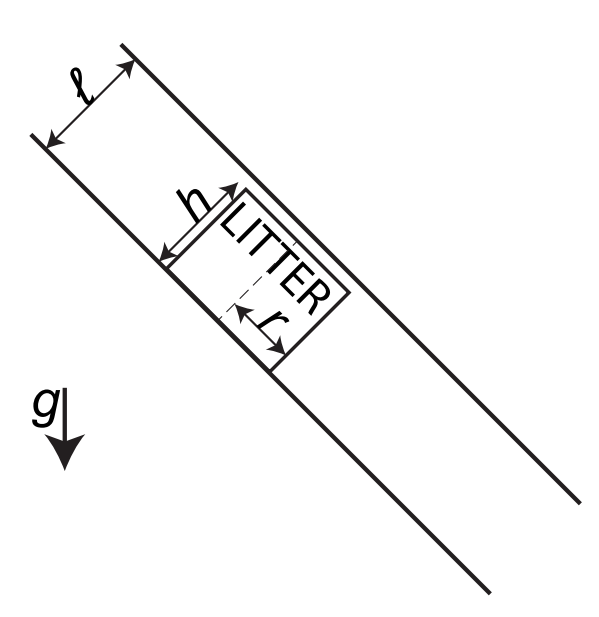
\includegraphics[width=0.5\linewidth]{2013-v3p-04-yl.PNG}
\end{center}
\fi
}

% Ü109
\ylDisplay{Veeboiler} % Ülesande nimi
{Tundmatu autor} % Autor
{piirkonnavoor} % Voor
{2016} % Aasta
{P 5} % Ülesande nr.
{2} % Raskustase
{
% Teema: Soojusõpetus
\ifStatement
Kui majja ei tule eraldi soojaveetoru, siis üks võimalus sooja vee saamiseks on elektrilise läbivooluboileri kasutamine. Boileri võimsus $N = 5,0$ kW ja kasutegur $\eta = 80\%$. Külmaveekraanist tuleva vee temperatuur $t_0 = 14$ $^{\circ}C,$ dušist väljuva vee temperatuur $t = 40 ^{\circ}C$ Mitu liitrit $40 ^{\circ}$ vett võib maksimaalselt dušist väljuda ühes minutis? Vee erisoojus on $c = 4200 J kg \cdot K$ ja tihedus $\rho = 1000 kg/m^3$.
\fi
}


% Ü110
\ylDisplay{Jääst kuup} % Ülesande nimi
{Tundmatu autor} % Autor
{lõppvoor} % Voor
{2016} % Aasta
{P 4} % Ülesande nr.
{2} % Raskustase
{
% Teema: Soojusõpetus
\ifStatement
Jääst kuubi sees on $V = 0,1$ $dm^3$ suurune tühimik. Kuubi temperatuur on $T_0 = 0^{\circ}C$. Kuubi sisse viiakse aeglaselt peene toru kaudu $m_a = 10$ grammi $100 ^{\circ}C$ veeauru. Kui suur tühimik (jäätumata osa) on jääst kuubi sees pärast soojusvahetuse lõppemist? Jää tihedus on $\rho_j = 0,9$ $g/cm^3$ , jää sulamissoojus $\lambda = 340$ kJ/kg, vee keemissoojus $L = 2300$ kJ/kg ning vee erisoojus $c = 4200 J/(kg \cdot ^{\circ}C)$. Soojusvahetust ümbritseva keskkonnaga pole vaja arvestada. 
\fi
}

% Ü111
\ylDisplay{Tilkumine} % Ülesande nimi
{Tundmatu autor} % Autor
{lõppvoor} % Voor
{2017} % Aasta
{P 2} % Ülesande nr.
{2} % Raskustase
{
% Teema: Soojusõpetus
\ifStatement
Plastikanuma põhjas on $m_j = 100$ g jääd temperatuuriga $T_j = -10 ^{\circ}$C. Anuma kohal asuvad külma ja sooja vee kraanid, mis tilguvad. Külma vee kraanist tilgub iga ajavahemiku $t_k = 1$ s möödudes veetilk massiga $m_k = 0,3$ g ning temperatuuriga $T_k = 4 ^{\circ}$C. Sooja vee kraanist tilgub iga ajavahemiku $t_s = 2$ s möödudes veetilk massiga $m_s = 0,3$ g ning temperatuuriga $T_s = 40^{\circ}$C. Millise aja möödudes sulab ära kogu anumas olnud jää? Soojusvahetust väliskeskonnaga ning anuma soojusmahtuvust mitte arvestada. Jää sulamissoojus $\lambda = 330$ kJ/kg, jää erisoojus $c_j = 2100$ $J/(kg \cdot ^{\circ}C)$, vee erisoojus $c_v = 4200$ $J/(kg \cdot ^{\circ}C)$.
\fi
}

% Ü112
\ylDisplay{Saun} % Ülesande nimi
{Richard Luhtaru} % Autor
{piirkonnavoor} % Voor
{2020} % Aasta
{P 5} % Ülesande nr.
{2} % Raskustase
{
% Teema: Soojusõpetus
\ifStatement
Juhan ja Peeter on saunas ning Juhan viskab kuumale kivikerisele külma vett temperatuuriga $10^{\circ}C$. Peeter väidab, et Juhan jahutab kerise niimoodi ära ja ütleb Juhanile, et ta viskaks külma vee asemel kuuma vett temperatuuriga $60 ^{\circ}C$. Juhan aga väidab vastu, et külma ja kuuma vee kasutamisel ei ole erilist vahet (kerise jahtumise erinevus on väiksem kui $10\%$). Kui palju väheneb kerise temperatuur kummalgi juhul, kui visata sinna $V = 200$ $cm^3$ vett? Kas Juhanil on õigus? Vee tihedus $\rho = 1000$ $kg/m^3$ , erisoojus $c_v = 4200$  $\frac{J}{kg \cdot ^{\circ}C}$ ja aurustumissoojus $L = 2300$ $kJ/kg$. Kerisekivide erisoojus $c_k = 700$ $\frac{J}{kg \cdot ^{\circ}C}$ ja kogumass $M = 100$ $kg$. Võib eeldada, et keris on piisavalt kuum ja kogu vesi aurustub ära.
\fi
}

% Ü113
\ylDisplay{Saun} % Ülesande nimi
{Tundmatu autor} % Autor
{piirkonnavoor} % Voor
{2010} % Aasta
{P 9} % Ülesande nr.
{3} % Raskustase
{
% Teema: Soojusõpetus
\ifStatement
Talvel, kui väljas on $0 ^{\circ}$C, suudab saunahoone keris kütta sauna $90^{\circ}$C-ni. 
a) Hinnake, kui soojaks suudab keris sauna kutta, kui väljas on $-20^{\circ}$C.
Maja on joonmõõtmetelt 3 korda suurem kui saun, aga täpselt sama kuju ja sama paksusega seintega. Maja radiaatorid suudavad $-20^{\circ}$C välistemperatuuri juures kutta maja $15^{\circ}$C-ni. 
b) Hinnake, kui kõrgele tõuseks temperatuur majas, kui sinna viia täisvõimsusel kütma ka sauna keris. 
c) Kerise võimsus on $P = 4$ kW. Hinnake, kui suur on maja radiaatorite koguvõimsus. 
Märkus: Soojuskadude võimsus on võrdeline seinte pindalaga ja temperatuuride vahega sees ja väljas.
\fi
}

% Ü114
\ylDisplay{Küttesüsteem} % Ülesande nimi
{Tundmatu autor} % Autor
{piirkonnavoor} % Voor
{2012} % Aasta
{P 8} % Ülesande nr.
{3} % Raskustase
{
% Teema: Soojusõpetus
\ifStatement
Talvel siseneb koolimaja kuttesüsteemi vesi algtemperatuuriga $t_0 = 60^{\circ}$ C ning väljub sealt temperatuuriga $t_1 = 40^{\circ}$ C. Koolimaja soojuskadude võimsus on $N = 100$ kW. Kooli siseneva ja sealt väljuva veetoru sisediameeter on $D = 100$ mm. Leidke veevoolu kiirus neis torudes. Vee erisoojus $c = 4200 \frac{J}{(kg \cdot ^{\circ}C)}$, tihedus $\rho = 1000 kg/m^3$ .
\fi
}

% Ü115
\ylDisplay{Maja} % Ülesande nimi
{Autor} % Autor
{lõppvoor} % Voor
{2013} % Aasta
{P 6} % Ülesande nr.
{3} % Raskustase
{
% Teema: Soojusõpetus
\ifStatement
Maja koosneb kahest ühesugusest toast, mis on sümmeetrilised neid eraldava vaheseina suhtes. Mõlemas toas on radiaator võimsusega $P$. Väljas on temperatuur $T_0$. Kui lülitada sisse üks radiaator, siis pärast soojenemist on temperatuur radiaatoriga toas $T_1$ ja teises $T_2$. Leidke temperatuur $T_3$, milleni soojenevad toad, kui töötavad mõlemad radiaatorid. Eeldage, et soojusvahetuse võimsus pinnaühiku kohta on võrdeline temperatuuride vahega. Põrand ja lagi on hästi soojustatud. 
\begin{center}
	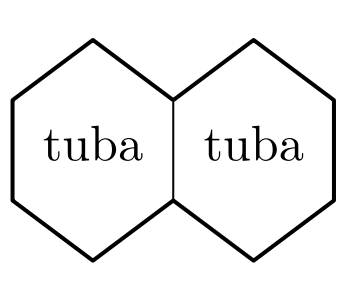
\includegraphics[width=0.5\linewidth]{2013-v3p-06-yl.PNG}
\end{center}
\fi
}

% Ü116
\ylDisplay{Jääst klaas} % Ülesande nimi
{Tundmatu autor} % Autor
{lõppvoor} % Voor
{2014} % Aasta
{P 5} % Ülesande nr.
{3} % Raskustase
{
% Teema: Soojusõpetus
\ifStatement
Jääst klaasi massiga $m_k = 20$ g ning temperatuuriga $t_0 = 0^{\circ}$C kallatakse $m_A=200$ g vedelikku $A$ temperatuuriga  $t_A = 25^{\circ}$C. Mitme protsendine vedeliku $A$ vesilahus tekib klaasis pärast soojusvahetuse lõppemist? Jää sulamissoojus $\lambda_{jaa} = 330$ kJ/kg, vedeliku $A$ erisoojus $c_A = 2400 J/kg \cdot ^{\circ}C$.
\fi
}

% Ü117
\ylDisplay{Vee kuumutamine} % Ülesande nimi
{Tundmatu autor} % Autor
{lõppvoor} % Voor
{2015} % Aasta
{P 7} % Ülesande nr.
{3} % Raskustase
{
% Teema: Soojusõpetus
\ifStatement
Pliidil olevas nõus kuumutatakse $M = 0,5$ kg vett. Vees olev termomeeter näitab, et vee temperatuur jääb püsivalt ühtlaseks $T_1 = 80 ^{\circ}$C juures. Vett kuumutatakse edasi ning vette lisatakse $m = 20$ g jää graanuleid (jää temperatuur on $T_{j} = 0 ^{\circ}$C, misjärel vee temperatuur hakkab enam-vähem püsiva kiirusega langema ning aja $t = 5,0$ min pärast on vee temperatuur langenud $T_2 = 75^{\circ}$C. Seejärel hakkab vee temperatuur tõusma ning tõuseb tagasi $T_1 = 80^{\circ}$C juurde, kus vee temperatuur enam ei muutu. Kui suure võimsusega kütab pliit potis olevat vett, eeldades et soojuskadude võimsus on võrdeline vee ja väliskeskkonna temperatuuride vahega. Õhu temperatuur on $T_0 = 20^{\circ}$C.
\fi
}

% Ü118
\ylDisplay{Soojusvaheti} % Ülesande nimi
{Tundmatu autor} % Autor
{lõppvoor} % Voor
{2016} % Aasta
{P 6} % Ülesande nr.
{3} % Raskustase
{
% Teema: Soojusõpetus
\ifStatement
Tagasivoolu soojusvahetis jahutatakse sissetulevat naftat temperatuuriga $T_n = 90 ^{\circ}C$ temperatuurini $20^{\circ}$C. Jahutusvesi liigub soojusvahetis vastupidises suunas naftaga ja siseneb soojusvahetisse temperatuuriga $T_v = 10 ^{\circ}C$. Vesi liigub kiirusega $v_v = 6 m^3/min$ ja nafta kiirusega $v_n = 15 m^3/min$. Leidke, millise temperatuuriga väljub soojusvahetist vesi? Vee erisoojus $c_v = 4200 \frac{J}{kg \cdot ^{\circ}C}$ , nafta erisoojus $c_n = 1800 \frac{J}{kg \cdot ^{\circ}C}$. Vee tihedus $\rho_v = 1000 kg/m^3$ ja nafta tihedus $\rho_n = 850$ $kg/m^3$
\fi
}

% Ü119
\ylDisplay{Kuulike vees} % Ülesande nimi
{EFO žürii} % Autor
{piirkonnavoor} % Voor
{2017} % Aasta
{P 9} % Ülesande nr.
{3} % Raskustase
{
% Teema: Soojusõpetus
\ifStatement
Jää-vee anumas ujuvad paksu jää kihiga kaetud vasest kuulikesed. Üks selline jääga kaetud kuulike (kogumassiga $m = 30$ g) asetatakse vette ruumalaga $V_v = 200$ ml ning temperatuuriga $T_v = 5 ^{\circ}$C. Mõne aja pärast vajub kuulike vee alla ning jääb sinna heljuma. Kui suur on vasest kuulikese mass $m_{Cu}$? Soojusvahetust väliskeskkonnaga mitte arvestada. Vee tihedus $\rho_v = 1,0$ $g/cm^3$ , jää tihedus $\rho_j = 0,9$ $g/cm^3$, vase tihedus $\rho_Cu = 9,0$ $g/cm^3$ vee erisoojus $c_v = 4200  \frac{J}{kg \cdot ^{\circ}C}$, vase erisoojus $c_{Cu} = 390 \frac{J}{kg \cdot ^{\circ}C}$, jää sulamissoojus $\lambda = 330$ kJ/kg.
\fi
}

% Ü120
\ylDisplay{Punker} % Ülesande nimi
{Mihkel Kree} % Autor
{piirkonnavoor} % Voor
{2017} % Aasta
{P 10} % Ülesande nr.
{3} % Raskustase
{
% Teema: Soojusõpetus
\ifStatement
Saarel toodab elektrit suletud punkrisse paigaldatud diiselgeneraator, mille soojuskadudest $P = 300$ W läheb punkri õhu soojendamiseks. Vältimaks punkri ülekuumenemist, paigaldakse ruumi ventilaator võimsusega $N = 5,0$ W, mis suunab õhku punkrist välja läbi toru sisediameetriga $d$. Kui suur peab olema toru läbimõõt $d$, et õhu temperatuur punkris ei ületaks $t_1 = 30$ $^{\circ}$C, samas kui välisõhu temperatuur on $t_0 = 20$ $^{\circ}$C? Soojuskadudega läbi punkri seinte mitte arvestada. Õhu tihedus $\rho = 1,2$ $kg/m^3$ ning erisoojus konstantsel rõhul $c_p = 1,0$ $\frac{kJ}{kg \cdot K}$.
\fi
}

% Ü121
\ylDisplay{Jää sulamine} % Ülesande nimi
{Koit Timpmann} % Autor
{lõppvoor} % Voor
{2018} % Aasta
{P 6} % Ülesande nr.
{3} % Raskustase
{
% Teema: Soojusõpetus
\ifStatement
Jäätükk massiga $m = 100$ g ja temperatuuriga $t_0 = 0^{\circ}$C ümbritseti soojusisolatsiooni kihiga ja paigutati hüdraulilise pressi alla, kus sellele jäätükile avaldati rõhku $p = 550$ atm ($1$ atm on rõhk, mis on võrdne õhurõhuga normaaltingimustel). Leidke selles protsessis tekkiva vee mass, kui on teada, et jää sulamistemperatuuri alanemine on võrdeline jääle avaldatud rõhuga ning rõhu suurenemisel $\triangle p = 138$ atm alaneb jää sulamistemperatuur $\triangle t = 1^{\circ}$C võrra. Jää erisoojus $c = 2100 J/(kg \cdot ^{\circ}C)$ ja sulamissoojus on $\lambda = 330$ kJ/kg.
\fi
}

% Ü122
\ylDisplay{Jääst nõu} % Ülesande nimi
{Erkki Tempel} % Autor
{lõppvoor} % Voor
{2018} % Aasta
{P 10} % Ülesande nr.
{3} % Raskustase
{
% Teema: Soojusõpetus
\ifStatement
Vees temperatuuriga $0^{\circ}$C ujub jääst kuup massiga $m_j = 1,5$ kg, mille sees on tühimik ruumalaga $V = 12$ $cm^3$. Tühimikku valatakse hästi aeglaselt elavhõbedat temperatuuriga $t$. Täpselt sel hetkel, kui tühimik täitub elavhõbedaga, vajub jääst kuup põhja. Leidke tühimikku kallatud elavhõbeda temperatuur $t$. Jää tihedus $\rho_j = 900$ $kg/m^3$ , vee tihedus $\rho_v = 1000$ $kg/m^3$, elavhõbeda tihedus $\rho_{Hg} = 13 600$ $kg/m^3$ , elavhõbeda erisoojus $c = 140$ $J/(kg\cdot ^{\circ}C)$, jää sulamissoojus $\lambda = 330$ kJ/kg. Soojusvahetust väliskeskkonnaga mitte arvestada.
\fi
}
\newpage\subsection{\protect\StrSubstitute{Valgusõpetus}{-}{ }}

% Ü123
\ylDisplay{Päiksekiir kaevupõhjas} % Ülesande nimi
{Tundmatu autor} % Autor
{piirkonnavoor} % Voor
{2000} % Aasta
{P 1} % Ülesande nr.
{1} % Raskustase
{
% Teema: Valgusõpetus
\ifStatement
Sügava kaevupõhja valgustamiseks päikesekiirtega kasutati tasapeeglit, mis oli paigutatud $25^{\circ}$ nurga all vertikaalsuuna suhtes. Kui suure nurga all maapinnast asus Päike?
\fi
}

% Ü124
\ylDisplay{Münt tassis} % Ülesande nimi
{Tundmatu autor} % Autor
{piirkonnavoor} % Voor
{2001} % Aasta
{P 1} % Ülesande nr.
{1} % Raskustase
{
% Teema: Valgusõpetus
\ifStatement
Tassi põhjas asub münt. Kui eemalduda tassist, siis teatud kaugusel kaob münt tassi serva varju. Kui aga nüüd valada tassi vett, siis võime uuesti münti samast vaatepunktist näha. Seletage antud nähtust.
\fi
}

% Ü125
\ylDisplay{Vedelikud} % Ülesande nimi
{Tundmatu autor} % Autor
{piirkonnavoor} % Voor
{2002} % Aasta
{P 2} % Ülesande nr.
{1} % Raskustase
{
% Teema: Valgusõpetus
\ifStatement
Klaasis on kaks kihti erinevat läbipaistvat vedelikku, mille vahel on terav horisontaalne piirjoon. Kuidas valguskiire abil teha kindlaks, kummas vedelikus on valguse levimise kiirus suurem?
\fi
}
 
 



% Ü126
\ylDisplay{Silm} % Ülesande nimi
{Tundmatu autor} % Autor
{piirkonnavoor} % Voor
{2004} % Aasta
{P 3} % Ülesande nr.
{1} % Raskustase
{
% Teema: Valgusõpetus
\ifStatement
Tasapeegel asub laual. Vaatame tasapeeglisse ja suleme ühe silma. Asetame peeglile 10-sendilise mundi nii, et see kataks suletud silma kujutise. Avame nüüd pead liigutamata suletud silma ja suleme teise silma. Kus asub nüüd münt näo kujutise suhtes? Põhjendage nähtut. Vahendid: tasapeegel, 10-sendine münt.
\fi
}

% Ü127
\ylDisplay{Peegeldused} % Ülesande nimi
{Tundmatu autor} % Autor
{piirkonnavoor} % Voor
{2006} % Aasta
{P 7} % Ülesande nr.
{1} % Raskustase
{
% Teema: Valgusõpetus
\ifStatement
Juku näeb peeglist hõõglambi kujutist (suunas A). Sama lambi kujutist märkab ta ka peegli ees olevalt peegeldavalt lauapinnalt (suunas B). Konstrueerige lambi asukoht eraldi lehel oleval joonisel.
\begin{center}
	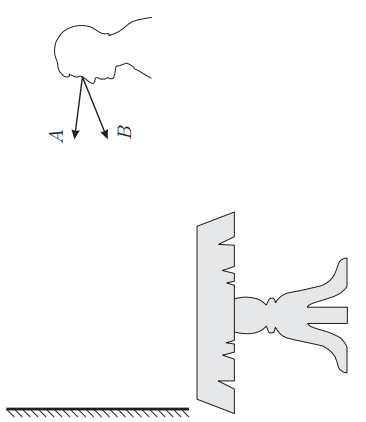
\includegraphics[width=0.5\linewidth]{2006-v2p-07-yl.PNG}
\end{center}
\fi
}


% Ü128
\ylDisplay{Autod peeglis} % Ülesande nimi
{Tundmatu autor} % Autor
{piirkonnavoor} % Voor
{2007} % Aasta
{P 4} % Ülesande nr.
{1} % Raskustase
{
% Teema: Valgusõpetus
\ifStatement
 Toas on vastasseintes maast laeni tasapeeglid. Kristi veeretab põrandal mänguautot risti peeglitega. Akki märkab ta, et peeglites on palju liikuvaid autosid. Milline on auto teise kujutise kiirus esimese kujutise suhtes kummaski peeglis, kui Kristi lükkab autot ühe peegli poole kiirusega $v = 0,5$ m/s?
\fi
}


% Ü129
\ylDisplay{Peeglid} % Ülesande nimi
{Autor} % Autor
{lõppvoor} % Voor
{2010} % Aasta
{P 1} % Ülesande nr.
{1} % Raskustase
{
% Teema: Valgusõpetus
\ifStatement
Kaks paralleelset tasapeeglit on paigutatud vastamisi vahekaugusega $d = 3$ m. Peeglite vahel seisev inimene näeb endast mitut kujutist, millest osa paikneb tema poole seljaga ja osa näoga. Kui kaugel paiknevad teineteisest kaks samas suunas vaatavat järjestikust kujutist?
\fi
}


% Ü130
\ylDisplay{Peegel} % Ülesande nimi
{Tundmatu autor} % Autor
{piirkonnavoor} % Voor
{2012} % Aasta
{P 1} % Ülesande nr.
{1} % Raskustase
{
% Teema: Valgusõpetus
\ifStatement
Suure ruumi seinal on $2,0 m$ laiune peegel. Peegli kõrval, $0,5 m$ kaugusel peeglist ja $1,0 m$ kaugusel seinast, seisab inimene. Mööda peegli keskjoont tuleb peegli poole tema tuttav. Kui kaugel peeglist on peeglile lähenev inimene, kui tuttavad märkavad teineteist peeglis?
\begin{center}
	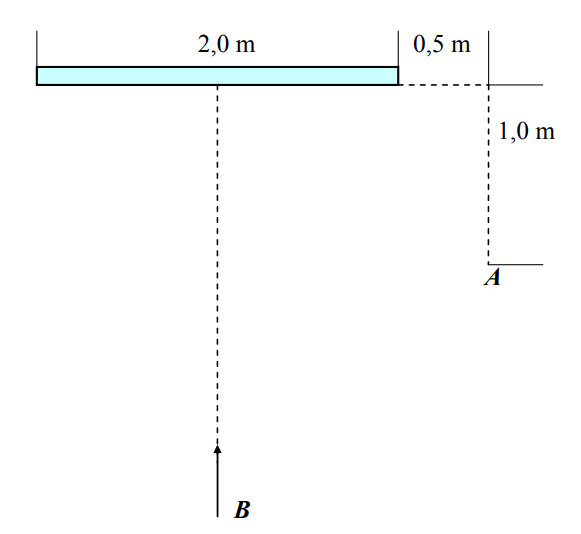
\includegraphics[width=0.5\linewidth]{2012-v2p-01-yl.PNG}
\end{center}
\fi
}


% Ü131
\ylDisplay{Küünlaleek} % Ülesande nimi
{Autor} % Autor
{lõppvoor} % Voor
{2012} % Aasta
{P 1} % Ülesande nr.
{1} % Raskustase
{
% Teema: Valgusõpetus
\ifStatement
Kõrgusega $h = 3,0$ cm küünlaleegi ja ekraani vahele paigutatakse õhuke kumerlääts nii, et ekraanile tekib leegi terav kujutis kõrgusega $h_1 = 6,0$ cm. Pärast läätse mõningat liigutamist tekkis ekraanile taas leegi terav kujutis. Leidke selle kõrgus $h_2$ nüüd.
\fi
}

% Ü132
\ylDisplay{Peegel} % Ülesande nimi
{Tundmatu autor} % Autor
{lõppvoor} % Voor
{2012} % Aasta
{P 8} % Ülesande nr.
{1} % Raskustase
{
% Teema: Valgusõpetus
\ifStatement
Joonisel on näidatud optiline süsteem, mis koosneb peeglist, koondavast läätsest, esemest ja valgust blokeerivast barjäärist. Konstrueerige lisalehel eseme tõeline kujutis.
\begin{center}
	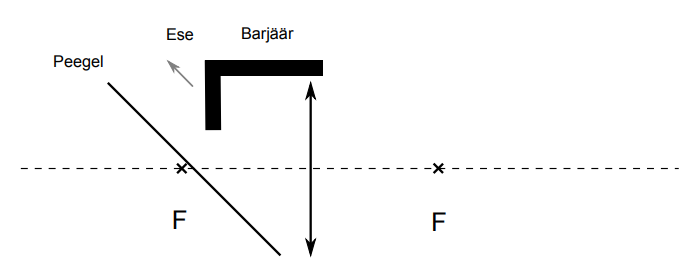
\includegraphics[width=0.5\linewidth]{2012-v3p-08-yl.PNG}
\end{center}
\fi
}


% Ü133
\ylDisplay{Lääts} % Ülesande nimi
{Tundmatu autor} % Autor
{piirkonnavoor} % Voor
{2013} % Aasta
{P 1} % Ülesande nr.
{1} % Raskustase
{
% Teema: Valgusõpetus
\ifStatement
Olgu meil kumerlääts optilise tugevusega $D = 10$ dptr. Kui kaugele läätsest tekib Kuu kujutis? Kui kaugele läätsest tekib Päikese kujutis? Kuu orbiidi raadiuseks võtta $r = 3,8 \cdot 105$ km, Maa orbiidi raadiuseks võtta $R = 1,5 \cdot 108$ km.
\fi
}
 


% Ü134
\ylDisplay{Kujutis kumerläätsega} % Ülesande nimi
{Tundmatu autor} % Autor
{piirkonnavoor} % Voor
{2014} % Aasta
{P 2} % Ülesande nr.
{1} % Raskustase
{
% Teema: Valgusõpetus
\ifStatement
Kumerläätsega tekitatakse valgusallika kujutis. Kui valgusallikas asub punktis $A$, tekib kujutis punktis $B$. Kui aga valgusallikas paigutada punkti $B$ tekib kujutis punktis $C$. Kas punkt $C$ langeb kokku punktiga $A$? Põhjendage. Valgusallika asukoha muutmisega ei muutu läätse asukoht.
\fi
}


% Ü135
\ylDisplay{Kujutis tasapeeglis} % Ülesande nimi
{Tundmatu autor} % Autor
{piirkonnavoor} % Voor
{2014} % Aasta
{P 3} % Ülesande nr.
{1} % Raskustase
{
% Teema: Valgusõpetus
\ifStatement
Kärbes lendab peegli poole kiirusega $v = 1$ $m/s$ nii, et kiirus on risti peegli tasandiga. Kui kiiresti peab peegel liikuma, et kärbse kujutis jääks paigale?
\fi
}

% Ü136
\ylDisplay{Kärbes peeglis} % Ülesande nimi
{Tundmatu autor} % Autor
{piirkonnavoor} % Voor
{2016} % Aasta
{P 1} % Ülesande nr.
{1} % Raskustase
{
% Teema: Valgusõpetus
\ifStatement
Kärbes lendab tasapeegli poole risti peegli pinnaga kiirusega $v$. Peegel liigub kulgevalt kärbse liikumisega samas suunas. Kui suure kiirusega $v'$ peaks liikuma peegel, et kärbse kujutis peeglis jääks liikumatuks?
\fi
}

% Ü137
\ylDisplay{Miku ja kärbes} % Ülesande nimi
{Tundmatu autor} % Autor
{piirkonnavoor} % Voor
{2003} % Aasta
{P 5} % Ülesande nr.
{2} % Raskustase
{
% Teema: Valgusõpetus
\ifStatement
Toa seinal on $1$ m laiune peegel. Miku seisab toas näoga seina poole, $3$ m kaugusel seinast ja $2$ m kaugusel peegli keskristsirgest. Akki näeb Miku peegli servas peeglist eemale lendava kärbse kujutist. Kui kiiresti peaks Miku taganema peegliga seinast eemale, et näha kogu 1 oma liikumise aja jooksul kärbse kujutist peegli servas, kui kärbes lendab piki peegli pinna keskristsirget peeglist eemale kiirusega $0,5$ m/s?
\begin{center}
	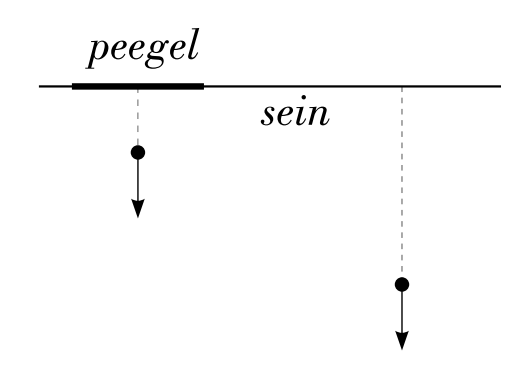
\includegraphics[width=0.5\linewidth]{2003-v2p-05-yl.PNG}
\end{center}
\fi
}
 


% Ü138
\ylDisplay{Akvaarium} % Ülesande nimi
{Tundmatu autor} % Autor
{piirkonnavoor} % Voor
{2009} % Aasta
{P 3} % Ülesande nr.
{2} % Raskustase
{
% Teema: Valgusõpetus
\ifStatement
Akvaariumi kohal on kaks punktvalgusallikat. Joonisel on näidatud kala vari ja poolvari akvaariumi põhjal. Lisalehel skitseerida punktvalgusallikate ligikaudsed asukohad.
\begin{center}
	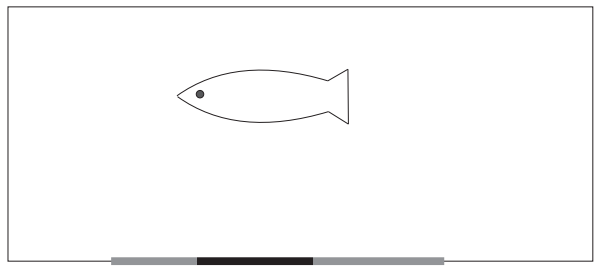
\includegraphics[width=0.5\linewidth]{2009-v2p-03-yl.PNG}
\end{center}
\fi
}


% Ü139
\ylDisplay{Tasapeeglid} % Ülesande nimi
{Tundmatu autor} % Autor
{piirkonnavoor} % Voor
{2011} % Aasta
{P 2} % Ülesande nr.
{2} % Raskustase
{
% Teema: Valgusõpetus
\ifStatement
Kaks vertikaalset tasapeeglit asuvad teineteise kõrval, küljed koos, peegelpinnad
$150^{\circ}$ nurga all. Uhele peeglile langeb $20^{\circ}$ nurga all peegelpinna suhtes peenike horisontaalne valgusvihk. Valgus peegeldub mõlemalt peeglilt. Mitme kraadi võrra on teiselt peeglilt peegeldunud valgusvihu suund erinev esimesele peeglile langenud valgusvihu suunast?
\fi
}


% Ü140
\ylDisplay{Valgusvihu laiendi} % Ülesande nimi
{Tundmatu autor} % Autor
{piirkonnavoor} % Voor
{2013} % Aasta
{P 5} % Ülesande nr.
{2} % Raskustase
{
% Teema: Valgusõpetus
\ifStatement
Laserist väljub paralleelne valgusvihk diameetriga $d = 2$ mm. Kasutades kumer- ja nõgusläätse muudetakse see paralleelseks valgusvihuks läbimõõduga $D = 6$ mm. Visandage optiline süsteem valgusvihu laiendamiseks ja arvutage nõgusläätse optiline tugevus, kui kasutatava kumerläätse fookuskaugus on $f = 15$ cm.
\fi
}


% Ü141
\ylDisplay{Läätsed} % Ülesande nimi
{Tundmatu autor} % Autor
{lõppvoor} % Voor
{2014} % Aasta
{P 3} % Ülesande nr.
{2} % Raskustase
{
% Teema: Valgusõpetus
\ifStatement
Optiline süsteem koosneb kumerläätsest fookuskaugusega $f_1$ ning nõgusläätsest fookuskaugusega $f_2$, kusjuures $f_1 = -4f_2$. Läätsed on paigutatud nii, et nende optilised peateljed ühtivad ning nende vaheline kaugus on $1,5f_1$. Ese asub kumerläätsest kaugusel $2f_1$. Konstrueerige eseme kujutis optilises süsteemis. 
\begin{center}
	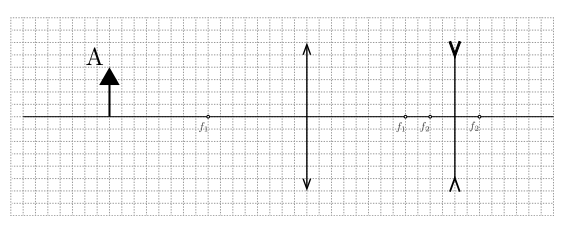
\includegraphics[width=0.5\linewidth]{2014-v3p-03-yl.PNG}
\end{center}
\fi
}
 


% Ü142
\ylDisplay{Hõbetatud lääts} % Ülesande nimi
{Tundmatu autor} % Autor
{lõppvoor} % Voor
{2016} % Aasta
{P 1} % Ülesande nr.
{2} % Raskustase
{
% Teema: Valgusõpetus
\ifStatement
Tasakumera läätse kumera tahu kõverusraadius on $50$ $cm$. Selle läätse optiline tugevus on $1$ $dpt$. Läätse kumer pind kaetakse hõbeda kihiga ning sellest tekib peegelpind. Kui suureks kujuneb selle keha optiline tugevus pärast kumera pinna hõbedaga katmist?
\fi
}


% Ü143
\ylDisplay{Läätsede süsteem} % Ülesande nimi
{EFO žürii} % Autor
{piirkonnavoor} % Voor
{2017} % Aasta
{P 4} % Ülesande nr.
{2} % Raskustase
{
% Teema: Valgusõpetus
\ifStatement
Kaks läätse optiliste tugevustega $D_1 = 10$ $dpt$ ja $D_2 = 5$ $dpt$ asuvad teineteisest $60$ $cm$ kaugusel. Läätsede optilised peateljed ühtivad. Ese asub esimese läätse ees, sellest $20$ $cm$ kaugusel optilisel peateljel. Kui kaugele teise läätse taha tekib optilise süsteemi poolt tekitatud kujutis, kui suur see on võrreldes esemega ning kas see on ümberpööratud või päripidine? 
\begin{center}
	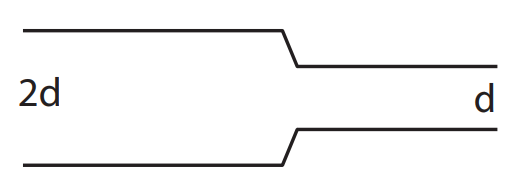
\includegraphics[width=0.5\linewidth]{2017-v2p-04-yl.PNG}
\end{center}
\fi
}


% Ü144
\ylDisplay{Optiline süsteem} % Ülesande nimi
{Tundmatu autor} % Autor
{lõppvoor} % Voor
{2017} % Aasta
{P 1} % Ülesande nr.
{2} % Raskustase
{
% Teema: Valgusõpetus
\ifStatement
Optiline süsteem koosneb kumerpeeglist ja kumerläätsest. Valguspunkt (taskulambipirni hõõgniit) asub kumerläätse optilisel peateljel läätsest kaugemal kui läätse fookuskaugus. Konstrueerige optilise süsteemi joonis, kus valguspunkti kujutis tekiks läätse fookusesse läätse ees. Selgitage lahendust.
\fi
}


% Ü145
\ylDisplay{Jope} % Ülesande nimi
{Andres Põldaru} % Autor
{piirkonnavoor} % Voor
{2019} % Aasta
{P 3} % Ülesande nr.
{2} % Raskustase
{
% Teema: Valgusõpetus
\ifStatement
Juku tahab peeglist vaadata, kuidas talle uus jope selga sobib. Peegel on aga väike ja sealt paistab ainult pool jopet. Põhjendage, kas peeglile lähemale/kaugemale minnes on jopet rohkem näha. 
\fi
}


% Ü146
\ylDisplay{Peegel} % Ülesande nimi
{Jaan Kalda} % Autor
{piirkonnavoor} % Voor
{2019} % Aasta
{P 5} % Ülesande nr.
{2} % Raskustase
{
% Teema: Valgusõpetus
\ifStatement
Optilises skeemis on kujutatud kolme valguskiire viit fragmenti. Samuti on teada, et skeemis on tasapeegel, mis on joonise tasandiga risti. Rekonstrueerige peegli asukoht. 
\begin{center}
	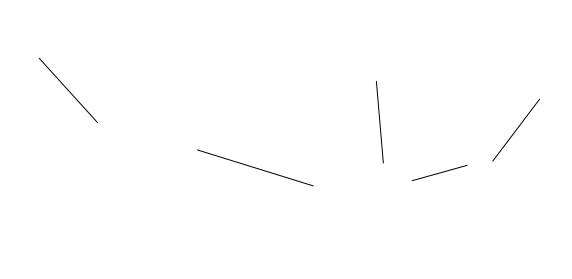
\includegraphics[width=0.5\linewidth]{2019-v2p-05-yl.PNG}
\end{center}
\fi
}


% Ü147
\ylDisplay{Prillid} % Ülesande nimi
{Autor} % Autor
{lõppvoor} % Voor
{2011} % Aasta
{P 8} % Ülesande nr.
{3} % Raskustase
{
% Teema: Valgusõpetus
\ifStatement
Juku on lühinägelik ja kasutab prille optilise tugevusega $D_1 = -4$ dpt. Ükskord proovis ta oma prillide asemel ette vanaema lugemisprille, mille optiline tugevus on $D_2 = +4$ dpt. Juku märkas, et vanaema prille kandes läheb pilt veel udusemaks, kuid neid peast teatud kaugusel hoides näeb ta ka kaugeid objekte teravalt. Mis oli prillide suurim kaugus silmast, mille korral Juku veel kaugeid objekte teravalt nägi? Mis oli läbi vanaema prillide nähtud pildi juures ebaharilik? Prille tavapärasel viisil kandes on silma kaugus prilliklaasist tühiselt väike.
\fi
}


% Ü148
\ylDisplay{Lääts} % Ülesande nimi
{Tundmatu autor} % Autor
{piirkonnavoor} % Voor
{2012} % Aasta
{P 10} % Ülesande nr.
{3} % Raskustase
{
% Teema: Valgusõpetus
\ifStatement
Klaasist kaksiknõgusa läätse optilisel peateljel paikneb väikeste mõõtmetega valgusallikas. Millist abivahendit, mis asub valgusallika ja nõgusläätse vahel, ja kuidas kasutades, saab nõgusläätse taha tekitada koonduva valgusvihu ja valgusallika tõelise kujutise? Põhjendage vastust joonisega.
\fi
}


% Ü149
\ylDisplay{Kujutis} % Ülesande nimi
{Tundmatu autor} % Autor
{piirkonnavoor} % Voor
{2013} % Aasta
{P 18} % Ülesande nr.
{3} % Raskustase
{
% Teema: Valgusõpetus
\ifStatement
Konstrueerige ruudu $ABCD$ kujutis kumerläätsega.
\begin{center}
	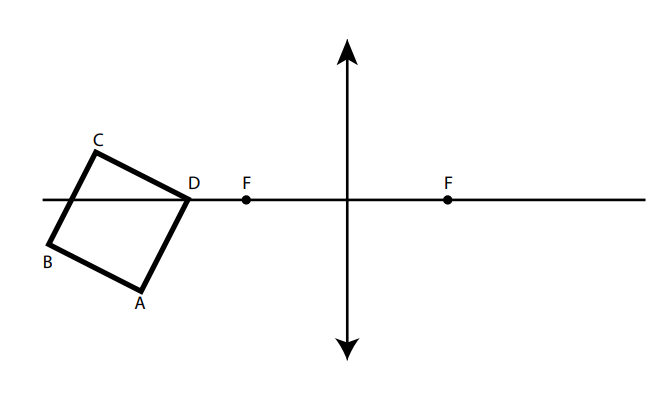
\includegraphics[width=0.5\linewidth]{2013-v2p-18-yl.PNG}
\end{center}
\fi
}

% Ü150
\ylDisplay{Läätsed} % Ülesande nimi
{Tundmatu autor} % Autor
{lõppvoor} % Voor
{2013} % Aasta
{P 7} % Ülesande nr.
{3} % Raskustase
{
% Teema: Valgusõpetus
\ifStatement
Jukul on suur hulk nõgusläätsi, mille fookuskauguste leidmiseks ta konstrueeris lihtsa
süsteemi. Ta suunas optilise peateljega paralleelse laserikiire läbimõõduga $2R$ tuntud
fookuskaugusega $f_1$ koondava läätse keskpunkti, pärast mida koondus laserkiir ühte punkti
ekraanil. Kui nüüd panna fookuskaugusega $f_2$ nõguslääts võrdsele kaugusele koondavast
läätsest ja ekraanist, on laserkiire läbimõõt ekraanil $2r$. Leidke $f_2$ eeldusel, et $2f_2 < f_1$.
\begin{center}
	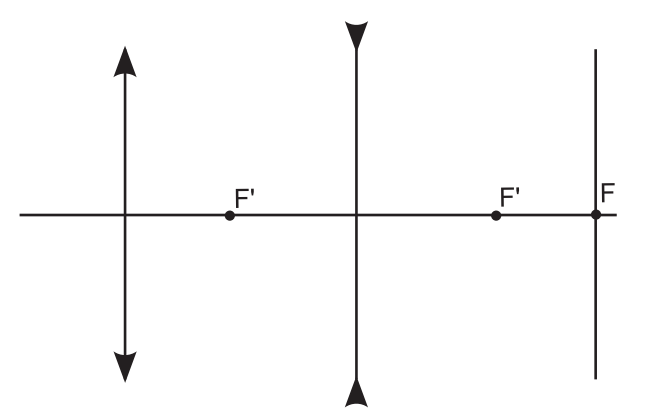
\includegraphics[width=0.5\linewidth]{2013-v3p-07-yl.png}
\end{center}
\fi
}

% Ü151
\ylDisplay{Projektor} % Ülesande nimi
{Tundmatu autor} % Autor
{lõppvoor} % Voor
{2013} % Aasta
{P 9} % Ülesande nr.
{3} % Raskustase
{
% Teema: Valgusõpetus
\ifStatement
Kodukinoprojektori paigutamisel võib tekkida olukord, kus kujutis tekib ekraani suhtes liiga kõrgele või madalale. Kui üritada kujutist projektori kallutamisega õigesse kohta nihutada, siis venib see trapetsikujuliseks. Mõned projektorid võimaldavad kujutise asukohta siiski ilma moonutusi tekitamata ristsuunas liigutada. Selleks nihutatakse projektori objektiivi optilise peateljega ristuvas suunas, jättes kõik ülejäänud detailid paigale. Vaatame lihtsat projektorit, mis koosneb kumerläätsest fookuskaugusega $f = 60$ $mm$ ja sellest teatud kaugusele paigutatud minikuvarist. Lääts tekitab endast $4L = 4$ $m$ kaugusele paigutatud ekraanile minikuvari terava suurendatud kujutise. Kui palju ja mis suunas tuleb läätse liigutada, et kujutis nihkuks ekraanil $\triangle$$Y$ = $20$ cm võrra kõrgemale?
\fi
}

% Ü152
\ylDisplay{Läätse skeem} % Ülesande nimi
{Tundmatu autor} % Autor
{piirkonnavoor} % Voor
{2014} % Aasta
{P 10} % Ülesande nr.
{3} % Raskustase
{
% Teema: Valgusõpetus
\ifStatement
Joonisel on kujutatud kaks sellist kiirt, mis lähtuvad punktvalgusallikast $A$ ning on läbinud läätse. Lääts asub sirgel $S$. Konstrueerige läätse fookuse asukoht.
\begin{center}
	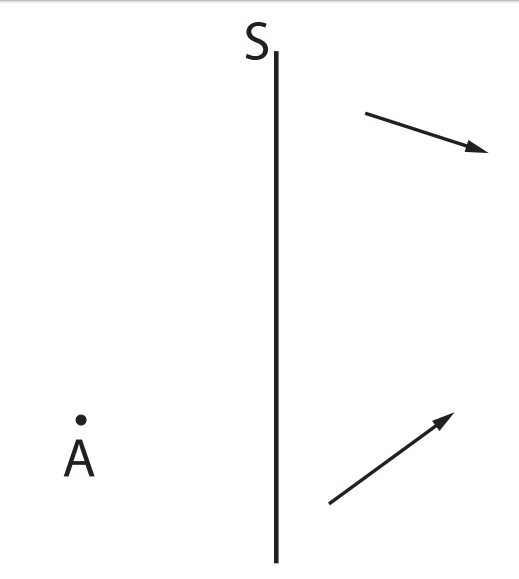
\includegraphics[width=0.5\linewidth]{2014-v2p-10-yl.PNG}
\end{center}
\fi
}


% Ü153
\ylDisplay{Kärbes peeglites} % Ülesande nimi
{Tundmatu autor} % Autor
{lõppvoor} % Voor
{2014} % Aasta
{P 7} % Ülesande nr.
{3} % Raskustase
{
% Teema: Valgusõpetus
\ifStatement
Kahe tasapeegi vaheline nurk on $120$$^{\circ}$  (vt joonist). Punktis $A$ asub vaatleja ning mööda sirget $s$ lendab edasi ja tagasi kärbes. Kärbse teatud asukohtade korral näeb vaatleja peeglites kahte kärbse kujutist. Tähistage sirgel $s$ see piirkond, mil tekib kaks kujutist.
\begin{center}
	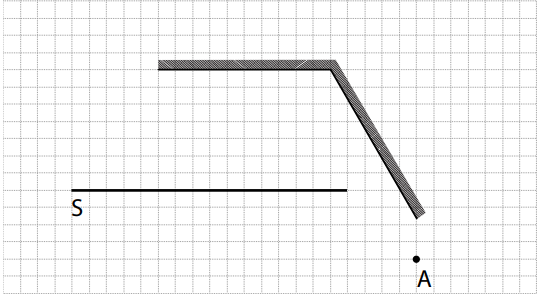
\includegraphics[width=0.5\linewidth]{2014-v3p-07-yl.PNG}
\end{center}
\fi
}


% Ü154
\ylDisplay{Läätse fookuskaugus} % Ülesande nimi
{Tundmatu autor} % Autor
{lõppvoor} % Voor
{2014} % Aasta
{P 9} % Ülesande nr.
{3} % Raskustase
{
% Teema: Valgusõpetus
\ifStatement
Nõguspeegliga puutub tihedalt kokku kumerlääts. Optilisel peateljel asub valguspunkt $S$. Valguspunktist väljuvad kiired läbivad läätse, peegelduvad peeglilt ja läbides uuesti läätse koonduvad samas punktis $S$. Arvutage läätse fookuskaugus, kui peegli kõverusraadius on $1$ m ja punkt $S$ asub läätsest $20$ cm kaugusel.
\fi
}

% Ü155
\ylDisplay{Laser ja lääts} % Ülesande nimi
{Tundmatu autor} % Autor
{lõppvoor} % Voor
{2015} % Aasta
{P 8} % Ülesande nr.
{3} % Raskustase
{
% Teema: Valgusõpetus
\ifStatement
Laser asub läätsest $2,5$ $f$ kaugusel ning optilisest peateljest kaugusel $f$, kus $f$ on läätse fookuskaugus. Laser on $45$$^{\circ}$ nurga all optilise peatelje suhtes. Teiselpool läätse olevale ekraanile tekib valgustäpp $0,5f$ võrra allpool optilist peatelge. Laserit liigutatakse paralleelselt peateljega $2f$ võrra läätse poole (laseri nurk ei muutu). Samal ajal liigutatakse ka ekraani paralleelselt optilise peateljega. Selle tulemusena asub valgustäpp ekraanil sama koha peal, kus alguses. Millise kauguse võrra nihutati ekraani? Kas oli võimalik, et ekraani ja laseri liigutamise ajal asus valgustäpp kogu aeg samas ekraani punktis?
\begin{center}
	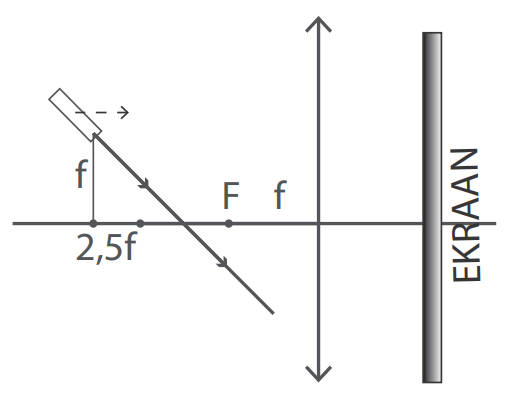
\includegraphics[width=0.5\linewidth]{2015-v3p-08-yl.PNG}
\end{center}
\fi
}

% Ü156
\ylDisplay{Ring ja ellips} % Ülesande nimi
{Tundmatu autor} % Autor
{lõppvoor} % Voor
{2015} % Aasta
{P 9} % Ülesande nr.
{3} % Raskustase
{
% Teema: Valgusõpetus
\ifStatement
Juuresoleval joonisel on kujutatud ring ja sellest koondava läätse poolt tekitatud kujutis. Leidke läätse keskpunkt, optiline peatelg ja fookus.
\begin{center}
	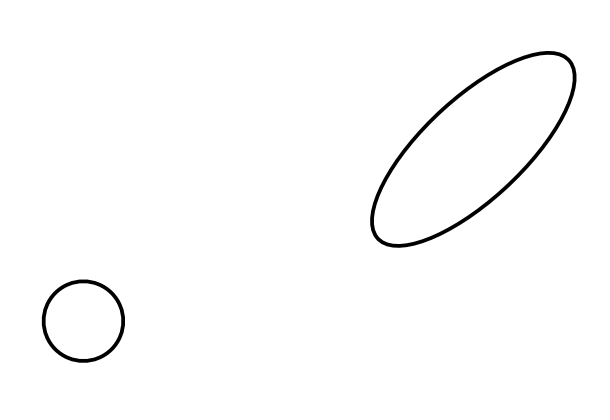
\includegraphics[width=0.5\linewidth]{2015-v3p-09-yl.PNG}
\end{center}
\fi
}


% Ü157
\ylDisplay{Nõguslääts} % Ülesande nimi
{Tundmatu autor} % Autor
{piirkonnavoor} % Voor
{2016} % Aasta
{P 7} % Ülesande nr.
{3} % Raskustase
{
% Teema: Valgusõpetus
\ifStatement
Punkt $A$ ja selle kujutis $A'$ asuvad läätse optilisest peateljest vastavalt $3$ cm ja $1$ cm kaugusel. Punkti $A$ ja selle kujutise kaugus mööda optilist peatelge on $10$ cm. Kui suur on läätse fookuskaugus, kui tegemist on nõgusläätsega?
\fi
}

% Ü158
\ylDisplay{Läätse fookus} % Ülesande nimi
{Tundmatu autor} % Autor
{piirkonnavoor} % Voor
{2016} % Aasta
{P 8} % Ülesande nr.
{3} % Raskustase
{
% Teema: Valgusõpetus
\ifStatement
Joonisel on näidatud punkt $A$, kus laserkiir lõikab pärast läätsede läbimist optilist peatelge. Konstrueerige nõgusläätse fookuse $F_n$ asukoht. Lahendage ülesanne lisalehel.
\begin{center}
	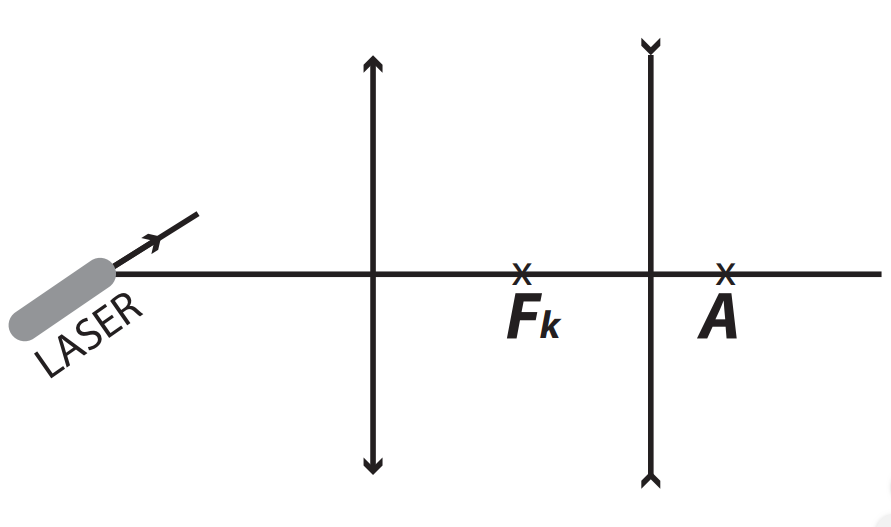
\includegraphics[width=0.5\linewidth]{2016-v2p-08-yl.PNG}
\end{center}
\fi
}


% Ü159
\ylDisplay{Sfäärilised peeglid} % Ülesande nimi
{Tundmatu autor} % Autor
{lõppvoor} % Voor
{2016} % Aasta
{P 10} % Ülesande nr.
{3} % Raskustase
{
% Teema: Valgusõpetus
\ifStatement
Joonisel on kujutatud kahe sfäärilise peegli optilised peateljed ja valguspunkti $A$ ja selle kujutise $A'$ asukohad kummagi peegli jaoks eraldi. Konstrueerige kummagi peegli pinna lõikepunkt optilise peateljega ja peeglite optilised keskpunktid.
\begin{center}
	\includegraphics[width=0.5\linewidth]{2016-v3p-10-yl.PNG}
\end{center}
\fi
}


% Ü160
\ylDisplay{Kujutis läätsega} % Ülesande nimi
{EFO žürii} % Autor
{piirkonnavoor} % Voor
{2017} % Aasta
{P 2} % Ülesande nr.
{3} % Raskustase
{
% Teema: Valgusõpetus
\ifStatement
Konstrueerige ese $AB$, mille kujutis $A'B'$ on antud. 
\begin{center}
	\includegraphics[width=0.5\linewidth]{2017-v2p-02-yl.PNG}
\end{center}
\fi
}


% Ü161
\ylDisplay{Diaprojektor} % Ülesande nimi
{EFO žürii} % Autor
{piirkonnavoor} % Voor
{2017} % Aasta
{P 6} % Ülesande nr.
{3} % Raskustase
{
% Teema: Valgusõpetus
\ifStatement
Diaprojektori objektiivi fookuskaugus on $40$ $mm$. Diapositiivi näitamisel on ekraanile tekkiv kujutis diapositiivist $80$ korda suurem. Kui kaugele objektiivi fokaaltasandist on paigutatud diapositiiv? Diapositiiv on sarnane fotoga, on üks kaader filmilindist, millel esemete värvused vastavad nende tegelikele värvustele ja mida diaprojektori abil saab projitseerida ekraanile.
\fi
}

% Ü162
\ylDisplay{Prillid} % Ülesande nimi
{Tundmatu autor} % Autor
{lõppvoor} % Voor
{2017} % Aasta
{P 7} % Ülesande nr.
{3} % Raskustase
{
% Teema: Valgusõpetus
\ifStatement
Kui Jüri loeb raamatut prillide abil, mille fookuskaugus on $2/3$ meetrit, hoiab ta raamatut $25$ cm kaugusel silmadest. Kui kaugel silmadest peab ta sama raamatut hoidma, et lugeda seda ilma prillideta pingutades silmi nagu eelmisel lugemisel.
\fi
}


% Ü163
\ylDisplay{Tasapinnaline plaat} % Ülesande nimi
{EFO žürii} % Autor
{piirkonnavoor} % Voor
{2018} % Aasta
{P 4} % Ülesande nr.
{3} % Raskustase
{
% Teema: Valgusõpetus
\ifStatement
Tasapinnaline plaat lõigati kaheks tükiks nagu on näidatud joonisel. Tekkisid kumerlääts ja nõguslääts. Pärast seda nihutati läätsed teineteisest eemale. Mis juhtub paralleelsete kiirte kimbuga, kui see langeb läätsede süsteemile: \\
a) koondava läätse poolt; \\
b) hajutava läätse poolt. \\
Kirjeldage juhte, kui läätsede vahemaa on fookuskaugusest suurem ja väiksem (Kokku neli juhtu).
\ifSolution
\begin{center}
	\includegraphics[width=0.5\linewidth]{2018-v2p-04-yl.PNG}
\end{center}
\fi
}


% Ü164
\ylDisplay{Paat} % Ülesande nimi
{Sandra Schumann} % Autor
{piirkonnavoor} % Voor
{2018} % Aasta
{P 7} % Ülesande nr.
{3} % Raskustase
{
% Teema: Valgusõpetus
\ifStatement
Juku on paadiga tiigil pindalaga $S = 20$ $m^2$ . Poiss viskab paadis oleva ankru vette. Leidke, kui palju ja mis suunas muutub veetase tiigis, kui 
\newline
a) ankrut paadiga ühendav tross on piisavalt pikk, et ankur toetuks tiigi põhja;
\newline
b) tross ei ole piisavalt pikk, et ankur toetuks tiigi põhja. Ankru ruumala koos trossiga $V_A = 0,003$ $m^3$ . Vee tihedus $\rho_v = 1000$ $kg/m^3$ ja ankru tihedus $\rho_A = 7900$ $kg/m^3$.
\fi
}

% Ü165
\ylDisplay{Kaks valgusallikat} % Ülesande nimi
{EFO žürii} % Autor
{piirkonnavoor} % Voor
{2018} % Aasta
{P 9} % Ülesande nr.
{3} % Raskustase
{
% Teema: Valgusõpetus
\ifStatement
Kaks punktikujulist valgusallikat asuvad kumerläätse optilisel peateljel erinevates punktides. Nendest valgusallikatest läätse abil tekitatud kujutised kattuvad. On teada, et üks valgusallikas asub läätse keskpunktist $a = 18$ cm kaugusel. Kui kaugel sellest valgusallikast asub teine valgusallikas? Läätse fookuskaugus $f = 9$ cm.
\fi
}


% Ü166
\ylDisplay{Kujutis} % Ülesande nimi
{EFO žürii} % Autor
{piirkonnavoor} % Voor
{2018} % Aasta
{P 10} % Ülesande nr.
{3} % Raskustase
{
% Teema: Valgusõpetus
\ifStatement
Joonisel on kujutatud läätse keskpunkt $O$, fookus $F$ ning kujutis $A'B'$ . Konstrueerige kujutise tekitanud ese.
\begin{center}
	\includegraphics[width=0.5\linewidth]{2018-v2p-10-yl.PNG}
\end{center}
\fi
}


% Ü167
\ylDisplay{Lääts ja selle fookus} % Ülesande nimi
{Koit Timpmann} % Autor
{lõppvoor} % Voor
{2018} % Aasta
{P 5} % Ülesande nr.
{3} % Raskustase
{
% Teema: Valgusõpetus
\ifStatement
Joonisel on kujutatud valguspunkt, sellest läätse abil saadud kujutis ning läätse optiline peatelg $O_1$$O_2$. Konstrueerige läätse ja selle fookuse asukohad kõikide võimalike juhtude jaoks. Esitage lahendus lisalehel.
\begin{center}
	\includegraphics[width=0.5\linewidth]{2018-v3p-05-yl.PNG}
\end{center}
\fi
}

% Ü168
\ylDisplay{Peegelpõhi} % Ülesande nimi
{Andra Schumann} % Autor
{lõppvoor} % Voor
{2018} % Aasta
{P 9} % Ülesande nr.
{3} % Raskustase
{
% Teema: Valgusõpetus
\ifStatement
Peegelpõhjaga tühja anumasse paigutatakse koondav klaaslääts nii, et läätse optiline peatelg on risti anuma põhjaga. Läätse kaugus anuma põhjast on $l = 10 cm$. Läätsele suunatakse paralleelne valgusvihk, mis koondub pärast läätse läbimist mingis punktis $A$. Siis valatakse anum vett täis (lääts jääb vee alla). Valgusvihk koondub endiselt samas punktis $A$. Leidke läätse fookuskaugus $f$ õhus. Klaasi murdumisnäitaja $n_k = 1,49$, vee murdumisnäitaja $n_v = 1,33$, õhu oma $n_0 = 1,0$. Murdumisnäitaja näitab, kui mitu korda on valguse kiirus vaakumis suurem kui aines.
\begin{center}
$f_v = f \cdot \cfrac{n_k n_v - n_0 n_v}{n_k n_0 - n_0 n_v}$
\end{center}
\fi
}

% Ü169
\ylDisplay{Näiv kujutis} % Ülesande nimi
{EFO žürii} % Autor
{piirkonnavoor} % Voor
{2019} % Aasta
{P 8} % Ülesande nr.
{3} % Raskustase
{
% Teema: Valgusõpetus
\ifStatement
Punktvalgusallikas asub läätse optilisel peateljel nii, et tekkinud näiv kujutis asub läätsele kaks korda lähemal kui valgusallikas. Leidke konstrueerimise teel läätse fookus.
\fi
}


% Ü170
\ylDisplay{Kärbes lendab} % Ülesande nimi
{EFO žürii} % Autor
{piirkonnavoor} % Voor
{2019} % Aasta
{P 9} % Ülesande nr.
{3} % Raskustase
{
% Teema: Valgusõpetus
\ifStatement
Kärbes asub kumerläätsest kümnekordse fookuskauguse kaugusel ning läätse optilisest peateljest kolme fookuskauguse kaugusel ning hakkab liikuma otse oma kujutise poole. Kui kaugel läätse tasandist asub kärbes hetkel, kui tema tõeline kujutis liigub kärbse suhtes \\
a) kõige aeglasemalt; \\
b) kõige kiiremini? Kui suur on kärbse kujutise kiirus nendel hetkedel?
\fi
}


% Ü171
\ylDisplay{Kujutise kiirus} % Ülesande nimi
{koit Timpmann} % Autor
{lõppvoor} % Voor
{2019} % Aasta
{P 5} % Ülesande nr.
{3} % Raskustase
{
% Teema: Valgusõpetus
\ifStatement
Punkt $A$ liigub kiirusega $v = 2$ cm/s risti läätse optilise peateljega. Kui suure kiirusega liigub selle punkti kujutis? Punkti $A$ projektsioon optilisele peateljele asub läätse keskpunktist $a = 15$ cm kaugusel ja läätse fookuskaugus $f = 10$ cm.
\begin{center}
	\includegraphics[width=0.5\linewidth]{2019-v3p-05-yl.PNG}
\end{center}
\fi
}

% Ü172
\ylDisplay{Kaksiklääts} % Ülesande nimi
{EFO žürii} % Autor
{piirkonnavoor} % Voor
{2020} % Aasta
{P 7} % Ülesande nr.
{3} % Raskustase
{
% Teema: Valgusõpetus
\ifStatement
Õhukese läätsega, mille optiline tugevuse $D = 5$ dpt tekitatakse ekraanile esemega täpselt sama suur kujutis. Nüüd asetatakse läätse kõrvale teine samasugune lääts (tekib kaksiklääts). Kui palju ja kuhu poole peab nihutama ekraani, et ekraanile tekiks uuesti terav kujutis?
\fi
}

% Ü173
\ylDisplay{Noole kujutis} % Ülesande nimi
{Oleg Košik} % Autor
{piirkonnavoor} % Voor
{2020} % Aasta
{P 8} % Ülesande nr.
{3} % Raskustase
{
% Teema: Valgusõpetus
\ifStatement
Konstrueerige noole $AB$ kujutis kumerläätses. Kas kujutis on tegelik või näiv?
\begin{center}
	\includegraphics[width=0.5\linewidth]{2020-v2p-08-yl.PNG}
\end{center}
\fi
}


% Ü174
\ylDisplay{Läätsede süsteem} % Ülesande nimi
{EFO žürii} % Autor
{piirkonnavoor} % Voor
{2020} % Aasta
{P 10} % Ülesande nr.
{3} % Raskustase
{
% Teema: Valgusõpetus
\ifStatement
Jüri tahtis ekraanile tekitada küünlaleegi suurendatud kujutist. Ta paigutas kumerläätse küünlaleegist kahekordse fookuskauguse kaugusele. Lähemale küünlale ta läätse panna ei saanud. Tekkinud kujutis ei olnud suurendatud. Jüri leidis kapist nõgusläätse ja asetanud selle kumerläätse ja ekraani vahele, saigi ekraanile küünlaleegi suurendatud kujutise. Joonistage valguskiirte käik Jüri katses ja vastake järgmisele küsimusele. Kuidas sõltub sellise skeemi korral kujutise suurus nõgusläätse fookuskaugusest?
\fi
}

\newpage\subsection{\protect\StrSubstitute{Võnkumine}{-}{ }}

% Ü175
\ylDisplay{Värvitilgad} % Ülesande nimi
{Tundmatu autor} % Autor
{piirkonnavoor} % Voor
{2009} % Aasta
{P 1} % Ülesande nr.
{1} % Raskustase
{
% Teema: Võnkumine
\ifStatement
Ühtlaselt ja sirgjooneliselt liikuva horisontaalse laua kohal on kaks paigalseisvat düüsi, millest tilgub lauale värvi. Värvitilgad langevad samast düüsist vvõrdsete ajavahemike järel. Joonisel on kujutatud teatud osa lauast värvitilkade jälgedega (täpid $A$, $B$, $C$, $D$). Mitu korda erinevad tilkade langemise sagedused (ajaühikus langenud tilkade arv) erinevatest düüsidest?
\begin{center}
	\includegraphics[width=0.5\linewidth]{2009-v2p-01-yl.PNG}
\end{center}
\fi
}

% Ü176
\ylDisplay{Maa pöörlemisperiood} % Ülesande nimi
{Tundmatu autor} % Autor
{piirkonnavoor} % Voor
{2014} % Aasta
{P 4} % Ülesande nr.
{2} % Raskustase
{
% Teema: Võnkumine
\ifStatement
Keskmiseks päikeseööpäevaks ehk tavatähenduses ööpäevaks nimetatakse keskmist perioodi, mille jooksul Päike näib Maaga seotud vaatleja jaoks tegevat taevas täisringi. Keskmise päikeseööpäeva pikkuseks on $24$ $h$ ehk $86 400$ $s$. Maal kulub ühe tiiru tegemiseks ümber Päikese $365,256$ keskmist päikeseööpäeva. Maa pöörlemissuund ümber oma telje ühtib selle tiirlemissuunaga Päikese ümber. Leidke nende andmete põhjal Maa pöörlemisperiood sekundi täpsusega.


\ifHint
Päikese näivat liikumist taevas põhjustavad nii Maa pöörlemine kui ka tiirlemine. Maa tiirlemise tõttu erineb Maa täispöörete arv aastas ühe võrra keskmiste päikeseööpäevade arvust. Kuna Maa tiirlemise suund ühtib Maa pöörlemise suunaga, siis teeb Maa ühe aasta jooksul ühe täispöörde rohkem.
\fi
}

% Ü177
\ylDisplay{Pendel} % Ülesande nimi
{Tundmatu autor} % Autor
{piirkonnavoor} % Voor
{2011} % Aasta
{P 10} % Ülesande nr.
{3} % Raskustase
{
% Teema: Võnkumine
\ifStatement
Pendel pandi väikese amplituudiga võnkuma ning stopperiga registreeriti neid hetki, kui pendel läbis vasakult poolt tulles oma tasakaalupunkti. Kaks järjestikust sellist sundmust toimusid hetkedel  $t_1 = 3,19$ s ja $t_2 =  5,64$ s. Pendlil lasti mõnda aega segamatult võnkuda, seejärel saadi kaheks järjestikuseks näiduks $t_3 =  61,14$ s ja $t_4 =  63,54$ s. Leidke võimalikult täpselt pendli võnkeperiood.
\fi
}

% Ü178
\ylDisplay{Kajalood} % Ülesande nimi
{Tundmatu autor} % Autor
{lõppvoor} % Voor
{2016} % Aasta
{P 5} % Ülesande nr.
{3} % Raskustase
{
% Teema: Võnkumine
\ifStatement
Vertikaalsuunas sukelduva allveelaeva kajalood kiirgab veekogu põhja suunas lühikesi heliimpulsse kestvusega $t_0$ sekundit. Põhjast tagasipeegeldunud registreeritud heliimpulsside kestvus on aga $t$ sekundit. Kui suur on allveelaeva sukeldumise kiirus $u$, kui heli levimise kiirus vees on $v$?
\fi
}


% Ü179
\ylDisplay{Film} % Ülesande nimi
{EFO žürii} % Autor
{piirkonnavoor} % Voor
{2019} % Aasta
{P 10} % Ülesande nr.
{3} % Raskustase
{
% Teema: Võnkumine
\ifStatement
Filmis näidatakse, kuidas poiss sõidab jalgrattaga. Kui poiss hakkab sõitma, veerevad rattad õiget pidi. Kiiruse kasvades paistavad rattad pöörlevat tagurpidi. Veel suurema kiiruse $v = v_0$ puhul näib, nagu ei pöörleks rattad üldse. Leidke kiirus $v_0$, kui on teada, et ratta ümbermõõt on $p = 2,5$ m ning rattal on $N = 36$ kodarat. Filmis vahetuvad kaadrid sagedusega $f = 24$ Hz (kaadrit sekundis).
\fi
}
\newpage\normalsize\section{Vihjed}
        \ToggleHint
        
% V1
\ylDisplay{Lüliti} % Ülesande nimi
{Tundmatu autor} % Autor
{piirkonnavoor} % Voor
{2012} % Aasta
{P 3} % Ülesande nr.
{1} % Raskustase
{
% Teema: Elektriõpetus

\ifHint
Toide on vaja lüliti plokile ühendada nii, et ühes asendis on plussklemm ühendatud mootori parema poolega ja miinusklemm vasaku poolega, et mootor töötaks ühtepidi, kuid teises asendis on pluss- ja miinusklemm ühendatud vastupidi, et mootor töötaks samuti vastassuunas.
\fi
}

% V2
\ylDisplay{Takistid} % Ülesande nimi
{Tundmatu autor} % Autor
{piirkonnavoor} % Voor
{2006} % Aasta
{P 6} % Ülesande nr.
{2} % Raskustase
{
% Teema: Elektriõpetus

\ifHint
Arvestada tuleb, et rööpühendusel on pinge konstantne ning jadaühendusel on kogupinge osapingete summa.
\fi
}

% V3
\ylDisplay{Takistite ühendused} % Ülesande nimi
{Tundmatu autor} % Autor
{piirkonnavoor} % Voor
{2008} % Aasta
{P 5} % Ülesande nr.
{2} % Raskustase
{
% Teema: Elektriõpetus

\ifHint
Kokku on võimalik takisteid ühendada 14 erinevat viisi.
\fi
}

% V4
\ylDisplay{Pirnid} % Ülesande nimi
{Tundmatu autor} % Autor
{piirkonnavoor} % Voor
{2009} % Aasta
{P 7} % Ülesande nr.
{2} % Raskustase
{
% Teema: Elektriõpetus

\ifHint
Võrdse nimipinge korral on nimivõimsused takistusega pöördvõrdelised.
\fi
}

% V5
\ylDisplay{Traat} % Ülesande nimi
{Tundmatu autor} % Autor
{piirkonnavoor} % Voor
{2010} % Aasta
{P 5} % Ülesande nr.
{2} % Raskustase
{
% Teema: Elektriõpetus

\ifHint
Lahendamisel tuleb lähtuda Ohm'i seadusest ja takistuse sõltuvusest materjalist, selle pikkusest ja ristlõike pindalast.
\fi
}

% V6
\ylDisplay{Vaskrõngas} % Ülesande nimi
{Tundmatu autor} % Autor
{piirkonnavoor} % Voor
{2011} % Aasta
{P 5} % Ülesande nr.
{2} % Raskustase
{
% Teema: Elektriõpetus

\ifHint
Rõnga kaared kui takistid on elektriliselt ühendatud rööbiti.
\fi
}


% V7
\ylDisplay{Küttekeha} % Ülesande nimi
{Tundmatu autor} % Autor
{lõppvoor} % Voor
{2012} % Aasta
{P 6} % Ülesande nr.
{2} % Raskustase
{
% Teema: Elektriõpetus

\ifHint
Maksimaalse võimsuse jaoks takistus minimeerida.
\fi
}

% V8
\ylDisplay{Skeem} % Ülesande nimi
{Tundmatu autor} % Autor
{lõppvoor} % Voor
{2013} % Aasta
{P 2} % Ülesande nr.
{2} % Raskustase
{
% Teema: Elektriõpetus

\ifHint
Ülesande lahendamisel aitab, kui skeem joonistada ümber lihtsamate jada- ja rööpühendustest koosneva segaühendusena.
\fi
}

% V9
\ylDisplay{Must kast} % Ülesande nimi
{Tundmatu autor} % Autor
{lõppvoor} % Voor
{2013} % Aasta
{P 5} % Ülesande nr.
{2} % Raskustase
{
% Teema: Elektriõpetus

\ifHint
Ülesande lahendusel piisab ainult kahe takisti lisamisest süsteemi.
\fi
}

% V10
\ylDisplay{Takistite võimsused} % Ülesande nimi
{Tundmatu autor} % Autor
{lõppvoor} % Voor
{2014} % Aasta
{P 6} % Ülesande nr.
{2} % Raskustase
{
% Teema: Elektriõpetus

\ifHint
Võimsus on võrdeline pinge ruudu ja pöördvõrdeline takistusega
\fi
}

% V11
\ylDisplay{Elektriskeem} % Ülesande nimi
{Tundmatu autor} % Autor
{lõppvoor} % Voor
{2014} % Aasta
{P 8} % Ülesande nr.
{2} % Raskustase
{
% Teema: Elektriõpetus

\ifHint
Ülesande lahendamisel aitab, kui skeem joonistada ümber lihtsamate jada- ja rööpühendustest koosneva segaühendusena.
\fi
}


% V12
\ylDisplay{Voltmeeter} % Ülesande nimi
{Tundmatu autor} % Autor
{piirkonnavoor} % Voor
{2016} % Aasta
{P 4} % Ülesande nr.
{2} % Raskustase
{
% Teema: Elektriõpetus

\ifHint
Leia esmalt rööpühenduse ja seejärel ahela kogutakistus ning seeläbi saad leida voolutugevuse.
\fi
}


% V13
\ylDisplay{Mõõtepiirkond} % Ülesande nimi
{Tundmatu autor} % Autor
{lõppvoor} % Voor
{2016} % Aasta
{P 3} % Ülesande nr.
{2} % Raskustase
{
% Teema: Elektriõpetus

\ifHint
Kuna pinge on nii mõõteriista kui ka takisti klemmidel sama suurusega, siis on voolutugevuste ja takistuste vaheline suhe sama.
\fi
}

% V14
\ylDisplay{Juhtmed} % Ülesande nimi
{Tundmatu autor} % Autor
{lõppvoor} % Voor
{2017} % Aasta
{P 4} % Ülesande nr.
{2} % Raskustase
{
% Teema: Elektriõpetus

\ifHint
Kuna tegemist on võrdlemisi pika ja peenikese juhtmega, siis peame me arvesse võtma juhtme takistust, mis on jadamisi lambi takistusega.
\fi
}

% V15
\ylDisplay{Must kast} % Ülesande nimi
{EFO žürii} % Autor
{piirkonnavoor} % Voor
{2019} % Aasta
{P 6} % Ülesande nr.
{2} % Raskustase
{
% Teema: Elektriõpetus

\ifHint
Kuna lüliti asend muudab takistust, siis peab lüliti ühendama süsteemist välja vähemalt ühe takisti nii, et süsteemist läheb vool ikkagi läbi.
\fi
}

% V16
\ylDisplay{Antikaitse} % Ülesande nimi
{Kaur Aare Saar} % Autor
{piirkonnavoor} % Voor
{2020} % Aasta
{P 9} % Ülesande nr.
{2} % Raskustase
{
% Teema: Elektriõpetus

\ifHint
Igal ajahetkel peab kogu pingelangus olema $240$ V.
\fi
}

% V17
\ylDisplay{Elektriküünlad} % Ülesande nimi
{Tundmatu autor} % Autor
{piirkonnavoor} % Voor
{2013} % Aasta
{P 7} % Ülesande nr.
{3} % Raskustase
{
% Teema: Elektriõpetus

\ifHint
Esmalt leia valgustite algne tegelik pinge ja võimsus, mis on väiksemad nimipingest ja -võimsusest.
\fi
}

% V18
\ylDisplay{Mobiililaadija} % Ülesande nimi
{Tundmatu autor} % Autor
{piirkonnavoor} % Voor
{2014} % Aasta
{P 8} % Ülesande nr.
{3} % Raskustase
{
% Teema: Elektriõpetus

\ifHint
Mehaaniline töö, mis on võrdeline inimese raskusjõuga ja talla kokku vajumisega, muundatakse elektrienergiaks, mis on võrdeline kasuteguri, pinge, voolutugevuse ja ajaga.
\fi
}

% V19
\ylDisplay{Voltmeeter} % Ülesande nimi
{Tundmatu autor} % Autor
{lõppvoor} % Voor
{2015} % Aasta
{P 3} % Ülesande nr.
{3} % Raskustase
{
% Teema: Elektriõpetus

\ifHint
Voltmeetri näidu saab leides esimese ja kolmanda takisti pingete vahe.
\fi
}

% V20
\ylDisplay{Kaks skeemi} % Ülesande nimi
{Tundmatu autor} % Autor
{lõppvoor} % Voor
{2015} % Aasta
{P 6} % Ülesande nr.
{3} % Raskustase
{
% Teema: Elektriõpetus

\ifHint
Takisti $R_1$ ja takisti $3R$ otstel olev pinge on sama, sest nad on ühendatud paralleelselt. Sama kehtib ka takistite $R_2$ ja $3R$ kohta.
\fi
}

% V21
\ylDisplay{Kaheksa} % Ülesande nimi
{Tundmatu autor} % Autor
{lõppvoor} % Voor
{2016} % Aasta
{P 9} % Ülesande nr.
{3} % Raskustase
{
% Teema: Elektriõpetus

\ifHint
Tehes skeemis ühe takistuse takistust väiksemaks, siis kogutakistus kas väheneb või jääb samaks.
\fi
}

% V22
\ylDisplay{Jõulutuled} % Ülesande nimi
{EFO žürii} % Autor
{piirkonnavoor} % Voor
{2017} % Aasta
{P 8} % Ülesande nr.
{3} % Raskustase
{
% Teema: Elektriõpetus

\ifHint
Alusta ülesande lahendamist kõikide lampide takistuste leidmisest.
\fi
}

% V23
\ylDisplay{Takistid} % Ülesande nimi
{Tundmatu autor} % Autor
{lõppvoor} % Voor
{2017} % Aasta
{P 8} % Ülesande nr.
{3} % Raskustase
{
% Teema: Elektriõpetus

\ifHint
Ülesande lahendamiseks on mõistlik esialgset skeemi lihtsustada, hinnates, millised vooluringi osad võiks skeemilt välja jätta ning millised saaks lihtsamateks osadeks taandada.
\fi
}

% V24
\ylDisplay{Pinge mõõtmine} % Ülesande nimi
{Tundmatu autor} % Autor
{lõppvoor} % Voor
{2017} % Aasta
{P 9} % Ülesande nr.
{3} % Raskustase
{
% Teema: Elektriõpetus

\ifHint
Kui oleks tegemist ideaalse voltmeetriga, siis peaks pinge jagunema takistite klemmidel proportsionaalselt, aga kuna mõõdetud pinge on sellest oluliselt väiksem, mõjutab mõõtmisi voltmeetri takistus. Voltmeetri takistuse leidmiseks tuleb kõigepealt leida voolutugevus takistites.
\fi
}

% V25
\ylDisplay{Takisti} % Ülesande nimi
{Jonathan Kalmus} % Autor
{piirkonnavoor} % Voor
{2018} % Aasta
{P 6} % Ülesande nr.
{3} % Raskustase
{
% Teema: Elektriõpetus

\ifHint
Takisti väärtus on voltmeetri sisetakistusega samas suurusjärgus ning seetõttu ei saa seda ignoreerida.
\fi
}

% V26
\ylDisplay{Päikesepaneelid} % Ülesande nimi
{Jonathan Kalmus} % Autor
{lõppvoor} % Voor
{2018} % Aasta
{P 3} % Ülesande nr.
{3} % Raskustase
{
% Teema: Elektriõpetus

\ifHint
Energiamahuti peab suutma talletada kogu päevase ületoodangu ehk selle osa paneelide poolt toodetud energiast, mida linn koheselt ära ei tarbi.
\fi
}

% V27
\ylDisplay{Vooluring} % Ülesande nimi
{Koit Timpmann} % Autor
{lõppvoor} % Voor
{2018} % Aasta
{P 7} % Ülesande nr.
{3} % Raskustase
{
% Teema: Elektriõpetus

\ifHint
Kuna juhtmel $CD$ takistus puudub, võime vooluringi punktid $C$ ja $D$ lugeda samaks, mille korral on kaks rööbiti ühendatud takistit ühendatud teise rööpühendusega jadamisi.
\fi
}

% V28
\ylDisplay{Elektriskeem} % Ülesande nimi
{EFO žürii} % Autor
{piirkonnavoor} % Voor
{2019} % Aasta
{P 7} % Ülesande nr.
{3} % Raskustase
{
% Teema: Elektriõpetus

\ifHint
Ruudu kaks vastastippu (ülemine ja alumine) on ka takistiga ühendatud, kuid selles takistis voolu ei ole. Skeemi ülemine ja alumine haru on sümmeetrilised, seega on pinge nii ülemise kui ka alumise haru esimese takisti otstel sama suur ning vertikaalselt paikneva takisti otstel pinge puudub. Seetõttu ei teki vertikaalselt paiknevas takistis elektrivoolu ning selle takisti takistust ei ole tarvis arvestada. Ruudu ülemiste takistite jada ja alumiste takistite jada on ühendatud rööbiti.
\fi
}

% V29
\ylDisplay{Kontuuri takistus} % Ülesande nimi
{Koit Timpmann} % Autor
{lõppvoor} % Voor
{2019} % Aasta
{P 7} % Ülesande nr.
{3} % Raskustase
{
% Teema: Elektriõpetus

\ifHint
Vooluahela paremaks mõistmiseks on mõistlik kujutada elektriskeem erinevate takistite rööp- ja jadaühendusskeemina.
\fi
}

% V30
\ylDisplay{Mikrokuumuti} % Ülesande nimi
{Valter Kiisk} % Autor
{lõppvoor} % Voor
{2019} % Aasta
{P 9} % Ülesande nr.
{3} % Raskustase
{
% Teema: Elektriõpetus

\ifHint
Takistuse leidmiseks temperatuuril $t_1 = 420 ^{\circ}C$ tuleb kasutada Ohm'i seadust ning seejärel saab etteantud valmitest avaldada otsitavad tegurid.
\fi
}

% V31
\ylDisplay{Trepp} % Ülesande nimi
{Tundmatu autor} % Autor
{lõppvoor} % Voor
{2011} % Aasta
{P 1} % Ülesande nr.
{1} % Raskustase
{
% Teema: Mehaanika

\ifHint
Kui esimene korrus asub maapinnal, siis teisele korrusele jõudmiseks tuleb tõusta ühe korruse võrra ja viiendale korrusele jõudmiseks on vaja tõusta $4$ korrust.
\fi
}


% V32
\ylDisplay{Liikumine} % Ülesande nimi
{Autor} % Autor
{lõppvoor} % Voor
{2011} % Aasta
{P 2} % Ülesande nr.
{1} % Raskustase
{
% Teema: Mehaanika

\ifHint
Ülevalpool ajatelge olev graafiku joon kirjeldab liikumist positiivses suunas, allpool ajatelge olev joon negatiivses suunas. Kuna liikumise iseloom igal etapil on erinev, tuleb arvutada iga etapi jooksul läbitud teepikkus arvestades ka liikumise suunda. Teepikkust võib arvutada graafiku joone ja ajatelje vahelise pindala kaudu.
\fi
}



% V33
\ylDisplay{Võidusõiduautod} % Ülesande nimi
{Tundmatu autor} % Autor
{piirkonnavoor} % Voor
{2012} % Aasta
{P 6} % Ülesande nr.
{1} % Raskustase
{
% Teema: Mehaanika

\ifHint
Keskmine kiirus on võrdne kogu teepikkuse ja kogu aja jagatisega.
\fi
}


% V34
\ylDisplay{Golfilöök} % Ülesande nimi
{Tundamtu autor} % Autor
{lõppvoor} % Voor
{2012} % Aasta
{P 2} % Ülesande nr.
{1} % Raskustase
{
% Teema: Mehaanika

\ifHint
Tuleb võtta arvesse, et heledaim valge täpp meile infot ei anna, sest see näitab vaid golfipalli algasendit enne seda, kui kepp teda lõi. Kahele järjestikkusele pildile on jäädvustunud heledast pallist paremale jäävad kaks tuhmimat valget palli kujutist. Nende ajaline vahe on $\tau$ ning me saame mõõta pallide vahekauguse joonlauaga.
\fi
}


% V35
\ylDisplay{Jõe ületamine} % Ülesande nimi
{Tundmatu autor} % Autor
{piirkonnavoor} % Voor
{2014} % Aasta
{P 1} % Ülesande nr.
{1} % Raskustase
{
% Teema: Mehaanika

\ifHint
Paadi liikumine koosneb kahest kompnendist: risti liikumine üle jõe ja allavoolu liikumine.
\fi
}

% V36
\ylDisplay{Ringrada} % Ülesande nimi
{Tundmatu autor} % Autor
{lõppvoor} % Voor
{2014} % Aasta
{P 1} % Ülesande nr.
{1} % Raskustase
{
% Teema: Mehaanika

\ifHint
Ülesande saab lahendada pelgalt loogilise arutluse teel ilma konkreetseid valemeid kasutamata.
\fi
}



% V37
\ylDisplay{Laua lükkamine} % Ülesande nimi
{Autor} % Autor
{lõppvoor} % Voor
{2014} % Aasta
{P 2} % Ülesande nr.
{1} % Raskustase
{
% Teema: Mehaanika

\ifHint
Vaadi ühe täispöördega liigub selle keskpunkt edasi vaadi ümbermõõduga võrdse teepikkuse võrra. Sama aja jooksul liigub laua vaadile toetuv ots vaadi keskpunkti suhtes edasi sama teepikkuse võrra. 
\fi
}


% V38
\ylDisplay{Helilaine} % Ülesande nimi
{Tundmatu autor} % Autor
{lõppvoor} % Voor
{2015} % Aasta
{P 1} % Ülesande nr.
{1} % Raskustase
{
% Teema: Mehaanika

\ifHint
Metallis, kus heli levib kiiremini, läbib heli poolrõngast teatud ajaga ning sama ajaga jõuab heli teises metallist mingile maale. Seejärel liiguvad need helid edasi koos samas metallis üksteisele vastu. Vastavatest kiiruse ja teepikkuse valemitest tuletades on võimalik avaldada heli liikumise kogu aeg.
\fi
}

% V39
\ylDisplay{Kera vees} % Ülesande nimi
{Autor} % Autor
{lõppvoor} % Voor
{2015} % Aasta
{P 2} % Ülesande nr.
{1} % Raskustase
{
% Teema: Mehaanika

\ifHint
Ülesande lahendamisel tuleb järgida põhimõtet, et kera poolt kausi põhjale mõjuv jõud on võrdne kera raskusjõu ja temale mõjuva üleslükkejõu vahega.
\fi
}

% V40
\ylDisplay{Rong} % Ülesande nimi
{Tundmatu autor} % Autor
{piirkonnavoor} % Voor
{2016} % Aasta
{P 2} % Ülesande nr.
{1} % Raskustase
{
% Teema: Mehaanika

\ifHint
Rongi poolt läbitud teepikkus on võrdne kiiruse graafiku aluse pindalaga.
\fi
}

% V41
\ylDisplay{Kaheksa} % Ülesande nimi
{EFO žürii} % Autor
{piirkonnavoor} % Voor
{2018} % Aasta
{P 2} % Ülesande nr.
{1} % Raskustase
{
% Teema: Mehaanika

\ifHint
Ülesande lahendamisel tuleb hinnata kui palju on droon $A$ teisest droonist taga pool ning millise suhtelise kiirusega ta seda vahemaad läbib.
\fi
}


% V42
\ylDisplay{Rongid} % Ülesande nimi
{EFO žürii} % Autor
{piirkonnavoor} % Voor
{2019} % Aasta
{P 1} % Ülesande nr.
{1} % Raskustase
{
% Teema: Mehaanika

\ifHint
Esimese ning teise rongi liikumiste kiiruste ja aegade korrutiste summa annab kokku linnade vahelise teepikkuse. Sellest seosest on võimalik avaldada kogu aeg. 
\fi
}

% V43
\ylDisplay{Päästerõngas} % Ülesande nimi
{EFO žürii} % Autor
{lõppvoor} % Voor
{2020} % Aasta
{P 1} % Ülesande nr.
{1} % Raskustase
{
% Teema: Mehaanika

\ifHint
Paatide kiirused ei ole tegelikult antud ülesandes üldse olulised. Lihtsustuse mõttes võib kujutada ka, et veevoolu ei eksisteeri ehk et paadid liiguvad seisvas vees.
\fi
}


% V44
\ylDisplay{Varras} % Ülesande nimi
{Tundmatu autor} % Autor
{lõppvoor} % Voor
{2011} % Aasta
{P 4} % Ülesande nr.
{2} % Raskustase
{
% Teema: Mehaanika

\ifHint
Sümmeetria tõttu on uues olukorras kumbki varda pool eraldi võetuna justkui esimeses situatsioonis: üks ots (varda keskkoht) jäigalt kinnitatud, teisele otsale (varda otspunkt) mõjub jõud $F/2$.
\fi
}


% V45
\ylDisplay{Lauatennisepall} % Ülesande nimi
{Tundmatu autor} % Autor
{lõppvoor} % Voor
{2011} % Aasta
{P 5} % Ülesande nr.
{2} % Raskustase
{
% Teema: Mehaanika

\ifHint
Vees mõjub pallile jõud, mis on võrdne üleslükkejõu ja raskusjõu vahega. Antud jõu tõttu omab pall potentsiaalset energiat veepinna nullnivoo suhtes. Samuti veest välja lennates maksimaalsel kõrgusel seistes, omab pallpotentsiaalset energiat, mis on veepõhjas olevast energiast väiksem siseenergia muutuse võrra.
\fi
}

% V46
\ylDisplay{Kolksatused} % Ülesande nimi
{Tundmatu autor} % Autor
{piirkonnavoor} % Voor
{2012} % Aasta
{P 5} % Ülesande nr.
{2} % Raskustase
{
% Teema: Mehaanika

\ifHint

\fi
}


% V47
\ylDisplay{Tünn} % Ülesande nimi
{Tundmatu autor} % Autor
{piirkonnavoor} % Voor
{2012} % Aasta
{P 7} % Ülesande nr.
{2} % Raskustase
{
% Teema: Mehaanika

\ifHint
Tühjale tünnile ja vedelikuga täidetud tünnile mõjuvad raskusjõud peavad olema võrdsed nendele tünnidele mõjuva üleslükke jõuga. Vedeliku tihedus on avaldatav vedeliku massist, mis lisatakse tünni.
\fi
}

% V48
\ylDisplay{Koer} % Ülesande nimi
{Tundmatu autor} % Autor
{lõppvoor} % Voor
{2012} % Aasta
{P 4} % Ülesande nr.
{2} % Raskustase
{
% Teema: Mehaanika

\ifHint
Lahenduse leidmiseks võiks punkti $P$ asemel kasutada tema peegeldust veepiiri suhtes $P'$ . Selliselt saab konstrueerida täisnurkse kolmnurga, mida lahendama hakata.
\fi
}

% V49
\ylDisplay{Ujuv anum} % Ülesande nimi
{Tundmatu autor} % Autor
{lõppvoor} % Voor
{2013} % Aasta
{P 1} % Ülesande nr.
{2} % Raskustase
{
% Teema: Mehaanika

\ifHint
Väiksem anum upub, kui ta vajub piisavalt sügavale, et vesi saaks hakata sisse voolama. Väikema anuma mass pluss anumas oleva vee mass peab olema võrdne üleslükkejõuga, et täita tasakaalutingimust.
\fi
}

% V50
\ylDisplay{Bussid} % Ülesande nimi
{Tundmatu autor} % Autor
{lõppvoor} % Voor
{2013} % Aasta
{P 3} % Ülesande nr.
{2} % Raskustase
{
% Teema: Mehaanika

\ifHint
Leia kahe järjestikuse bussi vahekaugus ning jalgratturi suhteline kiirus temale vastu liikuvate busside suhtes ning sealt saad leida, millise ajavahemiku tagant tuli talle buss vastu.
\fi
}

% V51
\ylDisplay{Parv} % Ülesande nimi
{Tundmatu autor} % Autor
{piirkonnavoor} % Voor
{2014} % Aasta
{P 5} % Ülesande nr.
{2} % Raskustase
{
% Teema: Mehaanika

\ifHint
Inimesele ja parvele mõjuvate raskusjõudude summa peab olema võrdne parvele mõjuva üleslükkejõuga.
\fi
}

% V52
\ylDisplay{Püstolkuulipilduja} % Ülesande nimi
{Tundmatu autor} % Autor
{piirkonnavoor} % Voor
{2014} % Aasta
{P 7} % Ülesande nr.
{2} % Raskustase
{
% Teema: Mehaanika

\ifHint
Kuuli lennuaeg võrdub kõrvalekaldega märgist jagatud rongide suhtelise kiirusega.
\fi
}

% V53
\ylDisplay{Liiklusummik} % Ülesande nimi
{Tundmatu autor} % Autor
{lõppvoor} % Voor
{2014} % Aasta
{P 4} % Ülesande nr.
{2} % Raskustase
{
% Teema: Mehaanika

\ifHint
Selleks, et leida kogu aega, tuleb hinnata, kui pikk vahemaa on tekkinud esimese ja viimase auto vahele selleks hetkeks, kui viimane auto saab liikuma hakata. Selle põhjal saab hinnata, kui kaua läbis esimene auto seda vahemaad ja kui kaua läbib viimane auto vahemaad ristmikuni.
\fi
}

% V54
\ylDisplay{Töö} % Ülesande nimi
{Tundmatu autor} % Autor
{piirkonnavoor} % Voor
{2016} % Aasta
{P 3} % Ülesande nr.
{2} % Raskustase
{
% Teema: Mehaanika

\ifHint
Keskmine võimsus on võrdelises seoses kogutööga ja pöördvõrdelises seoses kogu ajaga. Kogu aja saab avaldada esimese ja teise masina poolt tehtava töö ajast, mis omakorda avaldub kummagi masina töö ja võimsuse jagatisest.
\fi
}

% V55
\ylDisplay{Lennuk} % Ülesande nimi
{Tundmatu autor} % Autor
{lõppvoor} % Voor
{2016} % Aasta
{P 2} % Ülesande nr.
{2} % Raskustase
{
% Teema: Mehaanika

\ifHint
Kui lennuk sõidab tuulega samas sihis, siis ühes suunas tuleb lennuki tegeliku kiiruse leidmiseks lennuki kiirusest tuule kiirus lahutada ja teises suunas lennates kiirused omavahel liita. Kui tuul on risti lennusihiga, on lennuki tegelik kiirus lennuki ja tuule kiiruste ruutude vahe ruutjuur.
\fi
}

% V56
\ylDisplay{Rehvid} % Ülesande nimi
{EFO žürii} % Autor
{piirkonnavoor} % Voor
{2017} % Aasta
{P 1} % Ülesande nr.
{2} % Raskustase
{
% Teema: Mehaanika

\ifHint
Kuna $d_2$ on suurem kui $d_1$, siis valede rehvide korral sõidab auto kiiremini kui näitab spidomeeter.
\fi
}

% V57
\ylDisplay{Ujumine kanalis} % Ülesande nimi
{EFO žürii} % Autor
{piirkonnavoor} % Voor
{2017} % Aasta
{P 3} % Ülesande nr.
{2} % Raskustase
{
% Teema: Mehaanika

\ifHint
Kuna kanal on teises pooles kaks korda kitsam, kuid sama sügav, siis voolab seal vesi kaks korda kiiremini.
\fi
}

% V58
\ylDisplay{Kuulikesed} % Ülesande nimi
{EFO žürii} % Autor
{piirkonnavoor} % Voor
{2017} % Aasta
{P 5} % Ülesande nr.
{2} % Raskustase
{
% Teema: Mehaanika

\ifHint
Vasest kuulikeste mass peab olema võrdne kaadiumist kuulikeste ja vee massi summaga, et kangkaal oleks tasakaalus.
\fi
}

% V59
\ylDisplay{Rongid} % Ülesande nimi
{Autor} % Autor
{lõppvoor} % Voor
{2017} % Aasta
{P 3} % Ülesande nr.
{2} % Raskustase
{
% Teema: Mehaanika

\ifHint
Kui aja $t$ möödudes on reisirong jõudnud kaubarongile järele ja ei toimu kokkupõrget, siis on nende kiirused sel hetkel võrdsed. Kuna reisirongi kiirus muutus ühtlaselt, saame leida reisirongi keskmise kiiruse kaubarongile järelejõudmisel ja selle põhjal avaldada ka läbitud tee pikkuse.
\fi
}

% V60
\ylDisplay{Keha tihedus} % Ülesande nimi
{Autor} % Autor
{lõppvoor} % Voor
{2017} % Aasta
{P 5} % Ülesande nr.
{2} % Raskustase
{
% Teema: Mehaanika

\ifHint
Vette sukeldatud kehale mõjuva üleslükkejõu tõttu väheneb ka dünamomeeteri näit. Keha sukeldamisel vette surub keha välja oma ruumalaga võrdse koguse vett, mille tulemusel tõuseb veetase anumas ning suureneb rõhk anuma põhjale.
\fi
}


% V61
\ylDisplay{Jäätunud nael} % Ülesande nimi
{Autor} % Autor
{lõppvoor} % Voor
{2017} % Aasta
{P 6} % Ülesande nr.
{2} % Raskustase
{
% Teema: Mehaanika

\ifHint
Veetase muutub tänu sellele, et jää sulamisel selle ruumala väheneb. Vahetult enne uppumist on nael koos jääga pea täielikult vee all ning naela ja jää summaarne mass võrdub väljatõrjutud vedeliku massiga.
\fi
}

% V62
\ylDisplay{Jalgrattur} % Ülesande nimi
{EFO žürii} % Autor
{piirkonnavoor} % Voor
{2018} % Aasta
{P 1} % Ülesande nr.
{2} % Raskustase
{
% Teema: Mehaanika

\ifHint
Keskmine kiirus on kogu teepikkuse ja kogu aja jagatis.
\fi
}


% V63
\ylDisplay{Kaks kuulikest} % Ülesande nimi
{EFO žürii} % Autor
{piirkonnavoor} % Voor
{2018} % Aasta
{P 3} % Ülesande nr.
{2} % Raskustase
{
% Teema: Mehaanika

\ifHint
Kui joonestada graafik kiiruse ja aja vahelisest seosest, siis teepikkus graafikul on võrdne graafiku joone aluse viirutatud pindalaga.
\fi
}


% V64
\ylDisplay{Tanker} % Ülesande nimi
{Koit Timpmann} % Autor
{lõppvoor} % Voor
{2018} % Aasta
{P 1} % Ülesande nr.
{2} % Raskustase
{
% Teema: Mehaanika

\ifHint
Kui kaater liigub tankriga vastassuunas, siis tuleb kaatri ja tankri kiirused liita ning kui kaater liigub samas suunas, siis tuleb vastavad kiirused lahutada, et leida kaatri suhteline kiirus tenkri suhtes.
\fi
}

% V65
\ylDisplay{Kaks matkaselli} % Ülesande nimi
{Koit Timpmann} % Autor
{lõppvoor} % Voor
{2018} % Aasta
{P 2} % Ülesande nr.
{2} % Raskustase
{
% Teema: Mehaanika

\ifHint
Et jõuda laagrisse üheaegselt, peab kumbki matkasell pool teed läbima joostes ja pool jalgrattal.
\fi
}

% V66
\ylDisplay{Lennujaam} % Ülesande nimi
{Kristjan Kuppart} % Autor
{piirkonnavoor} % Voor
{2019} % Aasta
{P 4} % Ülesande nr.
{2} % Raskustase
{
% Teema: Mehaanika

\ifHint
Lihtsustuse mõttes võib antud liikumist vaadata hoopis seisvas taustsüsteemis.
\fi
}


% V67
\ylDisplay{Plokid} % Ülesande nimi
{Koit Timpmann} % Autor
{lõppvoor} % Voor
{2019} % Aasta
{P 3} % Ülesande nr.
{2} % Raskustase
{
% Teema: Mehaanika

\ifHint
Plokkide liikumisel kõrguste vahest tingitud potentsiaalse energia muutus muundub plokkide kineetiliseks energiaks. Plokkide kineetiliste energiate muutuste summa peab olema võrdne potentsiaalsete energiate muutumise summaga.
\fi
}

% V68
\ylDisplay{Rong} % Ülesande nimi
{Koit Timpmann} % Autor
{lõppvoor} % Voor
{2019} % Aasta
{P 22} % Ülesande nr.
{2} % Raskustase
{
% Teema: Mehaanika

\ifHint
Ülesande lahendamisele aitab kaasa kiiruse ja aja vahelist seost kuvava graafiku joonistamine. Kiiruse graafikul on keha poolt läbitud tee võrdne graafiku aluse pindalaga.
\fi
}

% V69
\ylDisplay{Bussid} % Ülesande nimi
{Moorits Mihkel Muru} % Autor
{piirkonnavoor} % Voor
{2020} % Aasta
{P 3} % Ülesande nr.
{2} % Raskustase
{
% Teema: Mehaanika

\ifHint
Esmalt tuleb leida, kui kaua kulub Jukul bussiga sõiduks aega ning siis hinnata, mitu bussi selle aja jooksul väljub. Lisaks peab arvesse võtma, et täpselt sama palju busse on juba enne sõitma hakkamist väljunud ning jõuavad tee peal Jukule vastu. Lõpuks veel lisaks ka see buss, mis väljus Jukuga samal ajal.
\fi
}


% V70
\ylDisplay{Kanali sild} % Ülesande nimi
{Eero Uustalu} % Autor
{piirkonnavoor} % Voor
{2020} % Aasta
{P 4} % Ülesande nr.
{2} % Raskustase
{
% Teema: Mehaanika

\ifHint
Silda koormab ainult tema peal paiknev vesi.
\fi
}

% V71
\ylDisplay{Jangtse kiirus} % Ülesande nimi
{EFO žürii} % Autor
{piirkonnavoor} % Voor
{2020} % Aasta
{P 6} % Ülesande nr.
{2} % Raskustase
{
% Teema: Mehaanika

\ifHint
Kuna vahemaa jääb samaks, siis on allavoolu liikumise suhtelise kiiruse ja aja korrutis võrdne ülesvoolu liikumise kiiruse ja aja korrutisega. Sellest võrdusest on võimalik avaldada laeva ja veevoolu kiiruste omavaheline suhe.
\fi
}

% V72
\ylDisplay{Kohtumispaik} % Ülesande nimi
{EFO žürii} % Autor
{lõppvoor} % Voor
{2020} % Aasta
{P 2} % Ülesande nr.
{2} % Raskustase
{
% Teema: Mehaanika

\ifHint
Ülesande lahendamise lähtuda sellest, et kohtumise hetkeks on mõlemad autod olnud liikvel koos pausidega võrdse aja. Mõlema auto liikumisvõrranditest saab avaldada aja ning panna need võrduma.
\fi
}


% V73
\ylDisplay{Plokid} % Ülesande nimi
{Tundmatu autor} % Autor
{lõppvoor} % Voor
{2012} % Aasta
{P 7} % Ülesande nr.
{3} % Raskustase
{
% Teema: Mehaanika

\ifHint
Mitmekordse jõu võidu saamiseks on vaja sellised plokisüsteemid panna üksteise suhtes järjestikku. Poolekordset võitu saab jällegi, kui ülesandes toodud süsteemi rakendada vastupidiselt.
\fi
}

% V74
\ylDisplay{Litter} % Ülesande nimi
{Tundmatu autor} % Autor
{lõppvoor} % Voor
{2012} % Aasta
{P 9} % Ülesande nr.
{3} % Raskustase
{
% Teema: Mehaanika

\ifHint
Sellest, et trajektoori madalaima ja kõrgeima punkti vahe vertikaalsuunas peab olema $2a$, saame leida ruudustiku sammuvahe.
\fi
}


% V75
\ylDisplay{Uppuv klots} % Ülesande nimi
{Tundmatu autor} % Autor
{lõppvoor} % Voor
{2012} % Aasta
{P 10} % Ülesande nr.
{3} % Raskustase
{
% Teema: Mehaanika

\ifHint
Korgile mõjub liiva raskusjõud ning altpoolt surub seda vesi. Kork kannatab nende jõudude vahet.
\fi
}

% V76
\ylDisplay{Vihm} % Ülesande nimi
{Tundmatu autor} % Autor
{piirkonnavoor} % Voor
{2013} % Aasta
{P 10} % Ülesande nr.
{3} % Raskustase
{
% Teema: Mehaanika

\ifHint
Seisvale inimesele langeb teatud kogus vett, mille ruumala on võrdne horisontaalsele pinnale langeva vee kogusega. Liikuval inimesel lisandub juurde läbi veepiiskade täidetud õhukõndimisel vertikaalse pinna komponent.
\fi
}

% V77
\ylDisplay{Klapp} % Ülesande nimi
{Tundmatu autor} % Autor
{lõppvoor} % Voor
{2013} % Aasta
{P 8} % Ülesande nr.
{3} % Raskustase
{
% Teema: Mehaanika

\ifHint
Et plaat ei eralduks toru otsast, peab olema täidetud tasakaalutingimus. Tasakaalutingimus on täidetud kui plaadile alt poolt mõjuv veerõhumisjõud on võrdne plaadile mõjuva raskusjõu ja õlisamba rõhumisjõu summaga.
\fi
}

% V78
\ylDisplay{Paadid} % Ülesande nimi
{Tundmatu autor} % Autor
{lõppvoor} % Voor
{2013} % Aasta
{P 10} % Ülesande nr.
{3} % Raskustase
{
% Teema: Mehaanika

\ifHint
Kolmnurkne paat on kahe prugiga ühel joonel, seetõttu pidid need sellest paadist olema kukkunud.
\fi
}


% V79
\ylDisplay{Lennukid} % Ülesande nimi
{Tundmatu autor} % Autor
{piirkonnavoor} % Voor
{2014} % Aasta
{P 9} % Ülesande nr.
{3} % Raskustase
{
% Teema: Mehaanika

\ifHint
Lahendus muutub lihtsaks, kui vaatleme ühe lennuki suhtelist liikumist teise suhtes ehk kui kujutame mõtteliselt punase lennukiga $B$ kaasaliikuvat taustsüsteemi.
\fi
}

% V80
\ylDisplay{Äpardus plokiga} % Ülesande nimi
{Tundmatu autor} % Autor
{lõppvoor} % Voor
{2014} % Aasta
{P 10} % Ülesande nr.
{3} % Raskustase
{
% Teema: Mehaanika

\ifHint
Alustuseks hinda anuma põhja poolt süsteemile "vesi pluss kehad" mõjuva jõu muutust. 
\fi
}

% V81
\ylDisplay{Kuup vedelikes} % Ülesande nimi
{Tundmatu autor} % Autor
{lõppvoor} % Voor
{2015} % Aasta
{P 4} % Ülesande nr.
{3} % Raskustase
{
% Teema: Mehaanika

\ifHint
Kuup asub sellisel sügavusel, et esineks jõudude tasakaal, kus kuubi raskusjõu ja kuubi ülemisele pinnale mõjuva vedeliku rõhumisjõu summa on võrdne vedeliku rõhumisjõuga kuubi alumisele pinnale.
\fi
}

% V82
\ylDisplay{Varras} % Ülesande nimi
{Tundmatu autor} % Autor
{lõppvoor} % Voor
{2015} % Aasta
{P 5} % Ülesande nr.
{3} % Raskustase
{
% Teema: Mehaanika

\ifHint
Niidile $EC$ mõjuv jõud on 2 korda suurem niidile $AD$ mõjuvast jõust ning need peavad olema tasakaalus vardale $DF$ tema keskpunktis mõjuva raskusjõuga.
\fi
}

% V83
\ylDisplay{Liiklejad} % Ülesande nimi
{Tundmatu autor} % Autor
{lõppvoor} % Voor
{2015} % Aasta
{P 10} % Ülesande nr.
{3} % Raskustase
{
% Teema: Mehaanika

\ifHint
Antsu, Birgiti ja Gerdi asukhad moodustavad igal ajahetkel võrdhaarse kolmnurga, mille alus asub Antsu ja Birgiti poolt kasutataval teel. Gerdi liikumine koosneb kahest komponendist: Antsu ja Birgitiga paralleelses sihis liikumisest ja nende liikumissuunaga risti liikumisest.
\fi
}

% V84
\ylDisplay{Kera vees} % Ülesande nimi
{Tundmatu autor} % Autor
{piirkonnavoor} % Voor
{2016} % Aasta
{P 6} % Ülesande nr.
{3} % Raskustase
{
% Teema: Mehaanika

\ifHint
Kehale mõjuv takistusjõud on vedelikus tõustes ja vajudes sama, kuid vastupidise suunaga.
\fi
}

% V85
\ylDisplay{Paat vees} % Ülesande nimi
{Tundmatu autor} % Autor
{piirkonnavoor} % Voor
{2016} % Aasta
{P 9} % Ülesande nr.
{3} % Raskustase
{
% Teema: Mehaanika

\ifHint
Vastuvoolu liikumisel tuleb suhtelise kiiruse leidmiseks lahutada paadi kiirusest veevoolu kiirus ja pärivoolu liikudes tuleb paadi ja veevoolu kiirus liita.
\fi
}

% V86
\ylDisplay{Kütusekulu linnas} % Ülesande nimi
{Tundmatu autor} % Autor
{piirkonnavoor} % Voor
{2016} % Aasta
{P 10} % Ülesande nr.
{3} % Raskustase
{
% Teema: Mehaanika

\ifHint
Kogu mootori poolt tehtud töö läheb peatumise järgselt autole kineetilise energia.
\fi
}

% V87
\ylDisplay{Glütseriin torus} % Ülesande nimi
{Autor} % Autor
{lõppvoor} % Voor
{2016} % Aasta
{P 7} % Ülesande nr.
{3} % Raskustase
{
% Teema: Mehaanika

\ifHint
Glütseriin ei voola välja, kui teeküünal püsib paigal, ehk selle alla ja üles mõjuvad jõud on tasakaalus.
\fi
}

% V88
\ylDisplay{Pidurdus} % Ülesande nimi
{Autor} % Autor
{lõppvoor} % Voor
{2016} % Aasta
{P 8} % Ülesande nr.
{3} % Raskustase
{
% Teema: Mehaanika

\ifHint
Auto kineetiline energia kulub pidurdusjõu ületamiseks ning potentsiaalse energia muuduks. Kõrguse muut ning auto poolt läbitud teepikkus on omavahel seotud avaldisega $\triangle h_1 = ks_1$.
\fi
}

% V89
\ylDisplay{Kalapüük} % Ülesande nimi
{EFO žürii} % Autor
{piirkonnavoor} % Voor
{2017} % Aasta
{P 7} % Ülesande nr.
{3} % Raskustase
{
% Teema: Mehaanika

\ifHint
Jaagu lisa kalapüügi ja kojusõiduaeg kokku on võrdne Jüri kojusõidu ajaga. Meeste kalapüügi kohtade kauguste arvutamisel peab arvestama ka veevoolu kiirusega liikumisel ja lisaks paatide triivimisega õngitsemise ajal.
\fi
}

% V90
\ylDisplay{Drooni vari} % Ülesande nimi
{Autor} % Autor
{lõppvoor} % Voor
{2017} % Aasta
{P 10} % Ülesande nr.
{3} % Raskustase
{
% Teema: Mehaanika

\ifHint
Ülesande lahendamiseks tee abistav joonis, mis kuvab drooni liikumise trajektoori ning varju liikumist maapinnal. Ülesande lahendus peitub täisnurksete kolmnurkade lahendamises.
\fi
}

% V91
\ylDisplay{Kontraktsioon} % Ülesande nimi
{EFO žürii} % Autor
{piirkonnavoor} % Voor
{2018} % Aasta
{P 5} % Ülesande nr.
{3} % Raskustase
{
% Teema: Mehaanika

\ifHint
Teades, piirituse massiprotsenti, saab esmalt leida vee ja piirituse masside suhte.
\fi
}

% V92
\ylDisplay{Kuup vedelikes} % Ülesande nimi
{Koit Timpmann} % Autor
{lõppvoor} % Voor
{2018} % Aasta
{P 4} % Ülesande nr.
{3} % Raskustase
{
% Teema: Mehaanika

\ifHint
Ülesannet on võimalik lahendada kahte pidi. Esimesel juhul mõistame, et kehale mõjuvad kolm jõudu - raskusjõud, vedeliku rõhk ülemisele pinnale ja vedeliku rõhk alumisele pinnale. Teisel juhul mõistame, et vedelikus heljuva keha korral võrdub kehale mõjuv raskusjõud kummagi vedeliku poolt mõjuvate üleslükkejõudude summaga
\fi
}


% V93
\ylDisplay{Veejuga} % Ülesande nimi
{Jonatan Kalmus} % Autor
{lõppvoor} % Voor
{2018} % Aasta
{P 8} % Ülesande nr.
{3} % Raskustase
{
% Teema: Mehaanika

\ifHint
Voolamisel kehtib massi jäävus ehk aja $\triangle t$ jooksul läbib pindu erinevaid veejoa ristlõikeid sama kogus vett. Setõttu peab muutuma veevoolu kiirus. Veevoolu kiiruse muutumise tingib potentsiaalse energia muutumine veejoa kõrguse vähenemisel.
\fi
}

% V94
\ylDisplay{Keha vees} % Ülesande nimi
{Koit Timpmann} % Autor
{lõppvoor} % Voor
{2019} % Aasta
{P 6} % Ülesande nr.
{3} % Raskustase
{
% Teema: Mehaanika

\ifHint
Pärast keha vettelaskmist mõjuvad parempoolsele kaalukausile järgmised jõud: statiivile mõjuv raskusjõud + kehale mõjuv raskusjõud – kehale mõjuv üleslükkejõud. Vasakule kaalukausile mõjub klaasile, veele ja keha poolt väljatõrjutud veele mõjuv raskusjõud.
\fi
}

% V95
\ylDisplay{Keha vees} % Ülesande nimi
{Jonatan Kalmus} % Autor
{lõppvoor} % Voor
{2019} % Aasta
{P 8} % Ülesande nr.
{3} % Raskustase
{
% Teema: Mehaanika

\ifHint
Joonisel oleva mõõtkava järgi saab võtta $500$ km vastava pikkuse joonisel. See pikkus tuleb võtta sirkli haarade vahele ja joonestada vastava raadiusega ringjooni märkides sirgjoonega lennuki võimalikke trajektoore.
\fi
}
 


% V96
\ylDisplay{Ühendatud anumad} % Ülesande nimi
{Kristjan Kuppart} % Autor
{lõppvoor} % Voor
{2019} % Aasta
{P 10} % Ülesande nr.
{3} % Raskustase
{
% Teema: Mehaanika

\ifHint
Süsteem on tasakaalus, kui teisse harusse lisandunud veesamba rõhk tasakaalustab õli ja puuklotsi lisamiseset tuleneva rõhu.
\fi
}

% V97
\ylDisplay{Palli soojenemine} % Ülesande nimi
{Tundmatu autor} % Autor
{piirkonnavoor} % Voor
{2013} % Aasta
{P 2} % Ülesande nr.
{1} % Raskustase
{
% Teema: Soojusõpetus

\ifHint
Energia, mis põrkel vabaneb ja muutub soojuseks, saab leida  potentisaalsete energiate vahest alguses ja pärast põrget.
\fi
}

% V98
\ylDisplay{Lumi} % Ülesande nimi
{Tundmatu autor} % Autor
{piirkonnavoor} % Voor
{2014} % Aasta
{P 6} % Ülesande nr.
{1} % Raskustase
{
% Teema: Soojusõpetus

\ifHint
Lumele vee lisamise lõppedes peab olema segu temperatuur $t = 0^{\circ}C$.
\fi
}

% V99
\ylDisplay{Vihm} % Ülesande nimi
{EFO žürii} % Autor
{piirkonnavoor} % Voor
{2018} % Aasta
{P 8} % Ülesande nr.
{1} % Raskustase
{
% Teema: Soojusõpetus

\ifHint
Sulava lumekihi kõrgus avaldub lume massist, mis on võrdne lume tiheduse, kõrguse ja pindala korrutisega. Sulava lume pindala on aga võrdne vihmavee pindalaga ning avaldub vihmavee massist ja selle jahtumisel eralduvast soojushulgast.
\fi
}

% V100
\ylDisplay{Külmkapp} % Ülesande nimi
{EFO žürii} % Autor
{piirkonnavoor} % Voor
{2019} % Aasta
{P 2} % Ülesande nr.
{1} % Raskustase
{
% Teema: Soojusõpetus

\ifHint
Külmkapp võimsusega $N$ peab tegema nelja tunni jooksul töö, mis on võrdne soojushulgaga, mis eraldub 1 liitri vee jahutamisel $ 0^{\circ}$C-ni ja poole liitri vee jäätumisel.
\fi
}

% V101
\ylDisplay{Mahl ja jää} % Ülesande nimi
{Erkki Tempel} % Autor
{lõppvoor} % Voor
{2019} % Aasta
{P 1} % Ülesande nr.
{1} % Raskustase
{
% Teema: Soojusõpetus

\ifHint
Soojustasakaalu saavutamiseks vajalik eneria saadakse mahla jahtumiselt. Mahla jahtumisel eraldunud energia kulub kolmeks protsessiks: jää soojendamiseks sulamistemperatuurini, jää sulatamiseks ja sulanud vee temperatuuri tõstmiseks.
\fi
}

% V102
\ylDisplay{Glütseriin} % Ülesande nimi
{Tundmatu autor} % Autor
{piirkonnavoor} % Voor
{2010} % Aasta
{P 7} % Ülesande nr.
{2} % Raskustase
{
% Teema: Soojusõpetus

\ifHint
Üleiigne ruumala glütseriini väljub ava kaudu, moodustades silindri pikkusega $v \triangle t$ ja ruumalaga $\triangle V = v S \triangle t$.
\fi
}

% V103
\ylDisplay{Radiaatorid} % Ülesande nimi
{Tundmatu autor} % Autor
{piirkonnavoor} % Voor
{2011} % Aasta
{P 8} % Ülesande nr.
{2} % Raskustase
{
% Teema: Soojusõpetus

\ifHint
Kuna mõlemat radiaatorit läbib ajaühikus võrdne kogus vett, määrab võimsuste suhte sisenevate ja väljuvate temperatuuride muutude suhe.
\fi
}

% V104
\ylDisplay{Bensiinikulu} % Ülesande nimi
{Tundmatu autor} % Autor
{piirkonnavoor} % Voor
{2012} % Aasta
{P 4} % Ülesande nr.
{2} % Raskustase
{
% Teema: Soojusõpetus

\ifHint
Ülesande lahendamisel tuleb leida, millise ajaga läbib auto 100 km ja seejärel leida, millise hulga tööd teeb antud mootor selle ajaga.
\fi
}

% V105
\ylDisplay{Külmunud tort} % Ülesande nimi
{Tundmatu autor} % Autor
{lõppvoor} % Voor
{2012} % Aasta
{P 3} % Ülesande nr.
{2} % Raskustase
{
% Teema: Soojusõpetus

\ifHint
Jää sulatamiseks vajalik soojushulk koosneb jää soojendamisest sulamistemperatuurini ja seejärel jää sulatamisest. Selle soojushulga annab jääle traadis elektrivoolu poolt tehtav töö.
\fi
}

% V106
\ylDisplay{Hõõrdkeevitus} % Ülesande nimi
{Tundamtu autor} % Autor
{lõppvoor} % Voor
{2012} % Aasta
{P 5} % Ülesande nr.
{2} % Raskustase
{
% Teema: Soojusõpetus

\ifHint
Hõõrdumisest tekkiv soojushulk on võrdne pöörlemisel tehtava tööga ehk hõõrdejõu ja pöörlemisel läbitud vahemaa korrutisega. See peab olema omakordne võrdne torude soojendamiseks vajamineva soojushulgaga.
\fi
}

% V107
\ylDisplay{Veepudel} % Ülesande nimi
{Tundmatu autor} % Autor
{piirkonnavoor} % Voor
{2013} % Aasta
{P 4} % Ülesande nr.
{2} % Raskustase
{
% Teema: Soojusõpetus

\ifHint
Ülesande põhiline idee seisneb selles, et vesi jäätub temperatuuril $0 ^{\circ}$C. Osa vee jäätumisel eralduvast soojushulgast läheb allajahtunud vee soojendamiseks jäätumistemperatuurile, seega tahkumisel eralduv soojushulk ja allajahtunud vee soojenemiseks kuluv energiahulk peavad olema võrdsed.
\fi
}

% V108
\ylDisplay{Litter} % Ülesande nimi
{Tundmatu autor} % Autor
{lõppvoor} % Voor
{2013} % Aasta
{P 4} % Ülesande nr.
{2} % Raskustase
{
% Teema: Soojusõpetus

\ifHint
Litri ühtlase kiirusega libisemisest järeldub, et kogu potentsiaalse energia muutus teisendub litri soojusenergiaks. 
\fi
}

% V109
\ylDisplay{Veeboiler} % Ülesande nimi
{Tundmatu autor} % Autor
{piirkonnavoor} % Voor
{2016} % Aasta
{P 5} % Ülesande nr.
{2} % Raskustase
{
% Teema: Soojusõpetus

\ifHint
Selleks, et leida millise koguse vett suudab boiler soojendada ühes minutis, tuleb leida millise kasuliku hulga energiat suudab boiler ühe minuti jooksul anda.
\fi
}


% V110
\ylDisplay{Jääst kuup} % Ülesande nimi
{Tundmatu autor} % Autor
{lõppvoor} % Voor
{2016} % Aasta
{P 4} % Ülesande nr.
{2} % Raskustase
{
% Teema: Soojusõpetus

\ifHint
Soojusvahetus lõppeb siis, kui veeaur on kondenseerunud ning jahtunud $^{\circ}C$-ni. Veeauru kondenseerumisel eraldunud soojushulk ning veeauru jahtumisel eraldunud soojushulk lähevad jää sulatamiseks $Q_j = Q_1 + Q_2$.
\fi
}

% V111
\ylDisplay{Tilkumine} % Ülesande nimi
{Tundmatu autor} % Autor
{lõppvoor} % Voor
{2017} % Aasta
{P 2} % Ülesande nr.
{2} % Raskustase
{
% Teema: Soojusõpetus

\ifHint
Kogu jää on sulanud siis, kui kraanidest tilkunud vesi on jahtunud $0 ^{\circ}C$-ni ning eraldunud soojus on läinud anumas oleva jää soojendamiseks $0 ^{\circ}C$-ni ning sulatamiseks.
\fi
}

% V112
\ylDisplay{Saun} % Ülesande nimi
{Richard Luhtaru} % Autor
{piirkonnavoor} % Voor
{2020} % Aasta
{P 5} % Ülesande nr.
{2} % Raskustase
{
% Teema: Soojusõpetus

\ifHint
Kerisekivide jahtumsiel eralduv soojushulk kulub vee soojendamiseks ja aurustamiseks. Sellest võrdsusest saame avaldada kerisekivide temperatuuride muudu.
\fi
}

% V113
\ylDisplay{Saun} % Ülesande nimi
{Tundmatu autor} % Autor
{piirkonnavoor} % Voor
{2010} % Aasta
{P 9} % Ülesande nr.
{3} % Raskustase
{
% Teema: Soojusõpetus

\ifHint
Kui tuba enam ei soojene, on kerise võimsus energia jäävuse seaduse järgi võrdne soojuskadude omaga. Antud seinte puhul määrab kadude võimsus üheselt temeratuurivahe sees ja väljas, sõltumata välistemperatuurist.
\fi
}

% V114
\ylDisplay{Küttesüsteem} % Ülesande nimi
{Tundmatu autor} % Autor
{piirkonnavoor} % Voor
{2012} % Aasta
{P 8} % Ülesande nr.
{3} % Raskustase
{
% Teema: Soojusõpetus

\ifHint
Ajavahemiku $\triangle t$ jooksul peavad radiaatorid andma koolimajale sama koguse soojust, mille kaotab koolimaja selle aja jooksul väliskeskkonda. Radiaatoritest eralduva soojushulga saab leida küttesüsteemi selle aja jooksul läbiva vee ruumala kaudu, millest saab omakorda avaldada veevoolu kiiruse.
\fi
}

% V115
\ylDisplay{Maja} % Ülesande nimi
{Autor} % Autor
{lõppvoor} % Voor
{2013} % Aasta
{P 6} % Ülesande nr.
{3} % Raskustase
{
% Teema: Soojusõpetus

\ifHint
Ülesannet on võimalik lahendada, kui avaldada tundmatu võrdetegur kuna soojusvahetuse võimsus pinnaühiku kohta on võrdeline temperaturride vahega peab ka soojusvahetus läbi terve seina olema võrdeline temperatuuride vahega. Ülesannet on ka võimalik lahendada lihtsamini kui märkame, et tegu on lineaarse süsteemiga ja teame, et lineaarse süsteemi korral kahe lahendi superpositsioon on samuti süsteemi lahend.
\fi
}

% V116
\ylDisplay{Jääst klaas} % Ülesande nimi
{Tundmatu autor} % Autor
{lõppvoor} % Voor
{2014} % Aasta
{P 5} % Ülesande nr.
{3} % Raskustase
{
% Teema: Soojusõpetus

\ifHint
Jääst klaas saab eneriat vedeliku $A$ jahtumisel eraldunud energia arvelt. Vabanenud energia läheb jääst klaasi sulamiseks.
\fi
}

% V117
\ylDisplay{Vee kuumutamine} % Ülesande nimi
{Tundmatu autor} % Autor
{lõppvoor} % Voor
{2015} % Aasta
{P 7} % Ülesande nr.
{3} % Raskustase
{
% Teema: Soojusõpetus

\ifHint
Ülesande lahendamiseks tuleb panna kirja võrrand, kus ühelt poolt vee jahtumisel eralduv energia ning pliidi poolt juurde antava energia summa peab olema võrdne jää sulamiseks, jää soojenemiseks ja soojuskadudeks kuluvate energiate summaga.
\fi
}

% V118
\ylDisplay{Soojusvaheti} % Ülesande nimi
{Tundmatu autor} % Autor
{lõppvoor} % Voor
{2016} % Aasta
{P 6} % Ülesande nr.
{3} % Raskustase
{
% Teema: Soojusõpetus

\ifHint
Nafta jahtumisel eraldunud soojus läheb vee soojendamiseks.
\fi
}

% V119
\ylDisplay{Kuulike vees} % Ülesande nimi
{EFO žürii} % Autor
{piirkonnavoor} % Voor
{2017} % Aasta
{P 9} % Ülesande nr.
{3} % Raskustase
{
% Teema: Soojusõpetus

\ifHint
Soojustasakaal saabub siis, kui vee temperatuur on $0^{\circ}C$. Seega saab leida sulanud jää massi. Kuna jääga kaetud kuulike heljub, siis peab tema keskmine tihedus olema võrdne vee tihedusega. Kuulikese keskmise tiheduse saame leida liites vase ja jää massi ning jagades selle nende ruumalade summaga. 
\fi
}

% V120
\ylDisplay{Punker} % Ülesande nimi
{Mihkel Kree} % Autor
{piirkonnavoor} % Voor
{2017} % Aasta
{P 10} % Ülesande nr.
{3} % Raskustase
{
% Teema: Soojusõpetus

\ifHint
Ventilaatori võimsus läheb toru läbivale õhule kineetilise energia andmiseks ning arvestame, et õhk liigub läbi ventilatsioonitoru kiirusega $v$. Tasakaalu korral peab ventilaatori kaudu väljuv õhk suutmata ära kanda kogu generaatorist eralduva soojusenergia.
\fi
}

% V121
\ylDisplay{Jää sulamine} % Ülesande nimi
{Koit Timpmann} % Autor
{lõppvoor} % Voor
{2018} % Aasta
{P 6} % Ülesande nr.
{3} % Raskustase
{
% Teema: Soojusõpetus

\ifHint
Esmalt tuleb leida jää sulamistemperatuur antud rõhul. Teiseks saame leida tekkiva vee massi võttes arvesse, et jää saab sulada vabanenud soojushulga arvelt.
\fi
}

% V122
\ylDisplay{Jääst nõu} % Ülesande nimi
{Erkki Tempel} % Autor
{lõppvoor} % Voor
{2018} % Aasta
{P 10} % Ülesande nr.
{3} % Raskustase
{
% Teema: Soojusõpetus

\ifHint
Teades, et uppumise korral on elavhõbedaga täidetud jääast kuubi keskmine tihedus võrdne vee tihedusega, saame leida lisatud elavhõbeda massi ning ruumala.
\fi
}

% V123
\ylDisplay{Päiksekiir kaevupõhjas} % Ülesande nimi
{Tundmatu autor} % Autor
{piirkonnavoor} % Voor
{2000} % Aasta
{P 1} % Ülesande nr.
{1} % Raskustase
{
% Teema: Valgusõpetus

\ifHint
Selleks, et valgustada sügava kaevu põhja, peab peeglilt peegeldunud kiir levima vertikaalselt alla.
\fi
}

% V124
\ylDisplay{Münt tassis} % Ülesande nimi
{Tundmatu autor} % Autor
{piirkonnavoor} % Voor
{2001} % Aasta
{P 1} % Ülesande nr.
{1} % Raskustase
{
% Teema: Valgusõpetus

\ifHint
Ülesande lahendus peitub murdumisseaduses.
\fi
}

% V125
\ylDisplay{Vedelikud} % Ülesande nimi
{Tundmatu autor} % Autor
{piirkonnavoor} % Voor
{2002} % Aasta
{P 2} % Ülesande nr.
{1} % Raskustase
{
% Teema: Valgusõpetus

\ifHint
Ülesande lahendus on seotud optilise tiheduse ja murdumisseadusega.
\fi
}
 
 



% V126
\ylDisplay{Silm} % Ülesande nimi
{Tundmatu autor} % Autor
{piirkonnavoor} % Voor
{2004} % Aasta
{P 3} % Ülesande nr.
{1} % Raskustase
{
% Teema: Valgusõpetus

\ifHint
Ülesande lihtsamaks lahendamiseks tuleb konstrueerida joonis ning lahendada probleem läbi tekkivate sarnaste kolmnurkade.
\fi
}

% V127
\ylDisplay{Peegeldused} % Ülesande nimi
{Tundmatu autor} % Autor
{piirkonnavoor} % Voor
{2006} % Aasta
{P 7} % Ülesande nr.
{1} % Raskustase
{
% Teema: Valgusõpetus

\ifHint
Lambi asukoha saab määrata kahe peegeldunud sirge lõikepunktiga. Esiteks tuleb pikendada suunas A lähtuvat kiirt ning see peegeldada peegeltasapinnalt vastavalt peegeldumisseadustele. Teiseks tuleb pikendada suuna B lähtuvat kiirt ning peegeldada seda nii laualt kui ka peegeltasapinnalt.
\fi
}


% V128
\ylDisplay{Autod peeglis} % Ülesande nimi
{Tundmatu autor} % Autor
{piirkonnavoor} % Voor
{2007} % Aasta
{P 4} % Ülesande nr.
{1} % Raskustase
{
% Teema: Valgusõpetus

\ifHint
Eimeses peeglis esimene kujutis läheneb temale ja teine kujutis kaugeneb temast. Mõlemad liiguvad kiirusega $v = 0,5$ m/s.
\fi
}


% V129
\ylDisplay{Peeglid} % Ülesande nimi
{Autor} % Autor
{lõppvoor} % Voor
{2010} % Aasta
{P 1} % Ülesande nr.
{1} % Raskustase
{
% Teema: Valgusõpetus

\ifHint
Samapidised on inimese kujutis peeglis ja selle kujutise teine kujutis.
\fi
}


% V130
\ylDisplay{Peegel} % Ülesande nimi
{Tundmatu autor} % Autor
{piirkonnavoor} % Voor
{2012} % Aasta
{P 1} % Ülesande nr.
{1} % Raskustase
{
% Teema: Valgusõpetus

\ifHint
Kõige kaugemal on inimene peeglist siis, kui tema peegeldust on näha peegli nurgast. Ülesanne lahendub siis sarnaste kolmnurkade kaudu.
\fi
}


% V131
\ylDisplay{Küünlaleek} % Ülesande nimi
{Autor} % Autor
{lõppvoor} % Voor
{2012} % Aasta
{P 1} % Ülesande nr.
{1} % Raskustase
{
% Teema: Valgusõpetus

\ifHint
Kui ese asub kaugusel $a$ läätsest ja tema tegelik kujutis kaugusel $b$ sellest, siis kiirte pööratavuse printsiibi kohaselt kui lääts paigutada kaugusele $b$ esemest, tekib tegelik kujutis kaugusele $a$ läätsest.
\fi
}

% V132
\ylDisplay{Peegel} % Ülesande nimi
{Tundmatu autor} % Autor
{lõppvoor} % Voor
{2012} % Aasta
{P 8} % Ülesande nr.
{1} % Raskustase
{
% Teema: Valgusõpetus

\ifHint
Kõige lihtsam viis ülesande lahendamiseks on kõigepealt konstrueerida eseme (näiv) kujutis peeglis ja konstrueerida sellest läätse abil tekkiv kujutis. Barjäär tagab, et tekib ainult üks tõeline kujutis.
\fi
}


% V133
\ylDisplay{Lääts} % Ülesande nimi
{Tundmatu autor} % Autor
{piirkonnavoor} % Voor
{2013} % Aasta
{P 1} % Ülesande nr.
{1} % Raskustase
{
% Teema: Valgusõpetus

\ifHint
Nii Kuu kui ka Päikese kaugus läätsest on väga suur, seega nendelt lähtunud kiired võib lugeda paralleelseteks
\fi
}
 


% V134
\ylDisplay{Kujutis kumerläätsega} % Ülesande nimi
{Tundmatu autor} % Autor
{piirkonnavoor} % Voor
{2014} % Aasta
{P 2} % Ülesande nr.
{1} % Raskustase
{
% Teema: Valgusõpetus

\ifHint
Ülesande lahendamiseks tuleb kirjeldada, kuidas tekivad kujutised kui ese asetada kuumerläätsel kaugemale kui läätse fookuskaugus ning kuidas siis kui asub läätsele lähemal kui fookuskaugus.
\fi
}


% V135
\ylDisplay{Kujutis tasapeeglis} % Ülesande nimi
{Tundmatu autor} % Autor
{piirkonnavoor} % Voor
{2014} % Aasta
{P 3} % Ülesande nr.
{1} % Raskustase
{
% Teema: Valgusõpetus

\ifHint
Kui mingi ajavahemiku vältel liigub peegel kärbsest eemale kauguse $s$ võrra, eemaldub kärbse kujutis peeglis kärbsest kauguse $2s$ võrra.
\fi
}

% V136
\ylDisplay{Kärbes peeglis} % Ülesande nimi
{Tundmatu autor} % Autor
{piirkonnavoor} % Voor
{2016} % Aasta
{P 1} % Ülesande nr.
{1} % Raskustase
{
% Teema: Valgusõpetus

\ifHint
Kui mingi ajavahemiku vältel liigub peegel kärbsest eemale kauguse $a$ võrra, eemaldub kärbse kujutis peeglis kärbsest kauguse $2a$ võrra.
\fi
}

% V137
\ylDisplay{Miku ja kärbes} % Ülesande nimi
{Tundmatu autor} % Autor
{piirkonnavoor} % Voor
{2003} % Aasta
{P 5} % Ülesande nr.
{2} % Raskustase
{
% Teema: Valgusõpetus

\ifHint
Ülesande lahendamisel tuleb konstrueerida joonis ning kasutada peegeldumise seadust ning kolmnurkade sarnasusi.
\fi
}
 


% V138
\ylDisplay{Akvaarium} % Ülesande nimi
{Tundmatu autor} % Autor
{piirkonnavoor} % Voor
{2009} % Aasta
{P 3} % Ülesande nr.
{2} % Raskustase
{
% Teema: Valgusõpetus

\ifHint
Kala varju ja poolvarju tekitavate kiirte konstrueerimisel tuleb arvestada ka valguse murdumisega veepiiril.
\fi
}


% V139
\ylDisplay{Tasapeeglid} % Ülesande nimi
{Tundmatu autor} % Autor
{piirkonnavoor} % Voor
{2011} % Aasta
{P 2} % Ülesande nr.
{2} % Raskustase
{
% Teema: Valgusõpetus

\ifHint
Ülesande lahendamiseks tasub teha joonis ning pikendada esialgset langevat kiirt ning viimast peegeldunud kiirt. Läbi pikenduste vahelise nurga saab määrata suuna erinevuse.
\fi
}


% V140
\ylDisplay{Valgusvihu laiendi} % Ülesande nimi
{Tundmatu autor} % Autor
{piirkonnavoor} % Voor
{2013} % Aasta
{P 5} % Ülesande nr.
{2} % Raskustase
{
% Teema: Valgusõpetus

\ifHint
Nõgusläätse ja kumerläätse fookused peavad kattuma.
\fi
}


% V141
\ylDisplay{Läätsed} % Ülesande nimi
{Tundmatu autor} % Autor
{lõppvoor} % Voor
{2014} % Aasta
{P 3} % Ülesande nr.
{2} % Raskustase
{
% Teema: Valgusõpetus

\ifHint
Konstrueerimisel peab järgima koondava kumerläätse ja hajutava nõgusläätse seaduspärasusi.
\fi
}
 


% V142
\ylDisplay{Hõbetatud lääts} % Ülesande nimi
{Tundmatu autor} % Autor
{lõppvoor} % Voor
{2016} % Aasta
{P 1} % Ülesande nr.
{2} % Raskustase
{
% Teema: Valgusõpetus

\ifHint
Tekib optiline süsteem, kus liituvad kumerläätse, nõguspeegli ja uuesti kumerläätse optilised tugevused.
\fi
}


% V143
\ylDisplay{Läätsede süsteem} % Ülesande nimi
{EFO žürii} % Autor
{piirkonnavoor} % Voor
{2017} % Aasta
{P 4} % Ülesande nr.
{2} % Raskustase
{
% Teema: Valgusõpetus

\ifHint
Optiliste tugevuste põhjal on võimalik arvutada läätsede fookuskaugused. Tuleb mõista, et kui ese asub kahe fookuskauguse kaugusel läätsest, asub ka selle kujutis kahe fookuskauguse kaugusel läätsest, on ümberpööratud ja eseme suurune.
\fi
}


% V144
\ylDisplay{Optiline süsteem} % Ülesande nimi
{Tundmatu autor} % Autor
{lõppvoor} % Voor
{2017} % Aasta
{P 1} % Ülesande nr.
{2} % Raskustase
{
% Teema: Valgusõpetus

\ifHint
Et kujutis tekiks peegli ees peegli fookuses, peavad peeglilt peegeldunud ja läätsele langevad kiired olema paralleelsed.
\fi
}


% V145
\ylDisplay{Jope} % Ülesande nimi
{Andres Põldaru} % Autor
{piirkonnavoor} % Voor
{2019} % Aasta
{P 3} % Ülesande nr.
{2} % Raskustase
{
% Teema: Valgusõpetus

\ifHint
Ülesande lahenduse paremaks selgitamiseks on mõistlik teha joonis.
\fi
}


% V146
\ylDisplay{Peegel} % Ülesande nimi
{Jaan Kalda} % Autor
{piirkonnavoor} % Voor
{2019} % Aasta
{P 5} % Ülesande nr.
{2} % Raskustase
{
% Teema: Valgusõpetus

\ifHint
Pane tähele, et ükski kiirefragment ei ole teisega samal sirgel. See tähendab, et kõikide kiirefragmentide puhul on tegemist kas erinevate kiirtega või sama kiire fragmentidega enne ja pärast peegeldumist. Et kiiri on kokku ainult kolm, siis vähemalt kaks fragmenti peavad olema pärit samalt kiirelt, üks enne ning teine pärast peegeldumist. 
\fi
}


% V147
\ylDisplay{Prillid} % Ülesande nimi
{Autor} % Autor
{lõppvoor} % Voor
{2011} % Aasta
{P 8} % Ülesande nr.
{3} % Raskustase
{
% Teema: Valgusõpetus

\ifHint
Lühinägelik silm näeb teravalt objekti, mis asub ei asu kaugmal teatud vahemaast. Prillide eesmärgiks on kaugest objektist tekitada kujutis, mis asub silmast samal kaugusel. Lõpmata kaugelt objektilt tulevad kiired on paralleelsed ja kujutise kaugus läätsest on võrdne fookuskauguse absoluutväärtusega.
\fi
}


% V148
\ylDisplay{Lääts} % Ülesande nimi
{Tundmatu autor} % Autor
{piirkonnavoor} % Voor
{2012} % Aasta
{P 10} % Ülesande nr.
{3} % Raskustase
{
% Teema: Valgusõpetus

\ifHint
Nõgusläätse ette tuleb paigutada koondav lääts, mille optiline peatelg ühtib nõgusläätse optilise peateljega.Koondava läätse optilise tugevuse arvuline väärtus peab olema suurem nõgusläätse optilise tugevuse arvulisest väärtusest, sest ainult sel juhul käitub kogu läätsede süsteem valgust koondavana.
\fi
}


% V149
\ylDisplay{Kujutis} % Ülesande nimi
{Tundmatu autor} % Autor
{piirkonnavoor} % Voor
{2013} % Aasta
{P 18} % Ülesande nr.
{3} % Raskustase
{
% Teema: Valgusõpetus

\ifHint
Kõige keerulisem on määrata punkti $D$ kujutise kaugust teisel pool läätse, sest see asub optilisel peateljel. Selleks võib võtta punktist $D$ optilise peateljega ühe ristsirge ning konstrueerida sellelt sirgelt mõne abipunkti kujutis teisele poole. Abipunkti kujutis peab olema samuti samal ristsirgel punkti $D$ kujutisega
\fi
}

% V150
\ylDisplay{Läätsed} % Ülesande nimi
{Tundmatu autor} % Autor
{lõppvoor} % Voor
{2013} % Aasta
{P 7} % Ülesande nr.
{3} % Raskustase
{
% Teema: Valgusõpetus

\ifHint
Kogu pilt on optilise peatelje suhtes sümmeetriline, tänu millele võib tegeleda ainult ühe poolega. Konstrueeri kiirte käik, teades et kõigi nõgusläätse läbivate paralleelsete kiirte pikendused lõikuvad fokaaltasandil.
\fi
}

% V151
\ylDisplay{Projektor} % Ülesande nimi
{Tundmatu autor} % Autor
{lõppvoor} % Voor
{2013} % Aasta
{P 9} % Ülesande nr.
{3} % Raskustase
{
% Teema: Valgusõpetus

\ifHint
Lihtsam on alguses vaadata olukorda, kus lääts on paigal ja liigutatakse minikuvarit. Suurendatud tõelise kujutise tekkimiseks peab minikuvar painema läätsest kaugusel, mis jääb ühe ja kahe fookuskauguse vahele.
\fi
}

% V152
\ylDisplay{Läätse skeem} % Ülesande nimi
{Tundmatu autor} % Autor
{piirkonnavoor} % Voor
{2014} % Aasta
{P 10} % Ülesande nr.
{3} % Raskustase
{
% Teema: Valgusõpetus

\ifHint
Lahenduseks piisab korrektse joonise olemasolust. Läbi läätse liikuvate kiirte lõikepunkti abil on võimalik konstrueerida fookust läbiva kiire liikumine.
\fi
}


% V153
\ylDisplay{Kärbes peeglites} % Ülesande nimi
{Tundmatu autor} % Autor
{lõppvoor} % Voor
{2014} % Aasta
{P 7} % Ülesande nr.
{3} % Raskustase
{
% Teema: Valgusõpetus

\ifHint
Sobiva piirkonna leidmisel tuleb arvestada kõikide võimalike piiripealsete punktidega ning leida nendes olevad kiirte peegeldumisnurgad.
\fi
}


% V154
\ylDisplay{Läätse fookuskaugus} % Ülesande nimi
{Tundmatu autor} % Autor
{lõppvoor} % Voor
{2014} % Aasta
{P 9} % Ülesande nr.
{3} % Raskustase
{
% Teema: Valgusõpetus

\ifHint
Kuna kiired lähtuvad punktist $S$ ja koonduvad uuesti punktis $S$, on $S$ optilise süsteemi fookuseks. Nõguspeegli ja kumerläätse optilised tugevused liituvad.
\fi
}

% V155
\ylDisplay{Laser ja lääts} % Ülesande nimi
{Tundmatu autor} % Autor
{lõppvoor} % Voor
{2015} % Aasta
{P 8} % Ülesande nr.
{3} % Raskustase
{
% Teema: Valgusõpetus

\ifHint
Ülesande lahendamisel tuleb kasutada kolmnurkade sarnasuse reegleid.
\fi
}

% V156
\ylDisplay{Ring ja ellips} % Ülesande nimi
{Tundmatu autor} % Autor
{lõppvoor} % Voor
{2015} % Aasta
{P 9} % Ülesande nr.
{3} % Raskustase
{
% Teema: Valgusõpetus

\ifHint
Läätse keskpunkti leiame kui ringile ja ellipsile tõmmatud puutujate lõikepunkti (puutepunktid peavad olema originaali-kujutise paarid ning neid ühendavad sirged peavad läbima läätse keskpunkti (sirged jooned joonisel).
\fi
}


% V157
\ylDisplay{Nõguslääts} % Ülesande nimi
{Tundmatu autor} % Autor
{piirkonnavoor} % Voor
{2016} % Aasta
{P 7} % Ülesande nr.
{3} % Raskustase
{
% Teema: Valgusõpetus

\ifHint
Ülesande lahendamiseks konstrueeri nõugusläätsesüsteemi kujutav joonis, kus tekkiv kujutis on näiline, samapidine ja vähendatud. Fookuskauguse leidmisel saad kasutada kolmnurkade sarnasust.
\fi
}

% V158
\ylDisplay{Läätse fookus} % Ülesande nimi
{Tundmatu autor} % Autor
{piirkonnavoor} % Voor
{2016} % Aasta
{P 8} % Ülesande nr.
{3} % Raskustase
{
% Teema: Valgusõpetus

\ifHint
Ülesande lahendamisel on vaja konstrueerida laserkiire liikumine läbi läätsede, kasutades selleks abisirgeid, mis on paralleelsed laserkiirega ning läbivad läätsede keskpunkte.
\fi
}


% V159
\ylDisplay{Sfäärilised peeglid} % Ülesande nimi
{Tundmatu autor} % Autor
{lõppvoor} % Voor
{2016} % Aasta
{P 10} % Ülesande nr.
{3} % Raskustase
{
% Teema: Valgusõpetus

\ifHint
Konstrueerimsiel lähtu peegeldumise seadustest.
\fi
}


% V160
\ylDisplay{Kujutis läätsega} % Ülesande nimi
{EFO žürii} % Autor
{piirkonnavoor} % Voor
{2017} % Aasta
{P 2} % Ülesande nr.
{3} % Raskustase
{
% Teema: Valgusõpetus

\ifHint
Esmalt tuleb joonistada risti läätsega tema keskpunkti läbiv optiline peatelg. Seejärel on võimalik "tagurpidi" konstrueerides kujutada eseme asukoht.
\fi
}


% V161
\ylDisplay{Diaprojektor} % Ülesande nimi
{EFO žürii} % Autor
{piirkonnavoor} % Voor
{2017} % Aasta
{P 6} % Ülesande nr.
{3} % Raskustase
{
% Teema: Valgusõpetus

\ifHint
Ülesande lahendamiseks tuleb koostada joonis ning lahendada see sarnaste kolmnurkade seostega.
\fi
}

% V162
\ylDisplay{Prillid} % Ülesande nimi
{Tundmatu autor} % Autor
{lõppvoor} % Voor
{2017} % Aasta
{P 7} % Ülesande nr.
{3} % Raskustase
{
% Teema: Valgusõpetus

\ifHint
Silma ja prilliläätse koos kasutamisel nende optilised tugevused liituvad.
\fi
}


% V163
\ylDisplay{Tasapinnaline plaat} % Ülesande nimi
{EFO žürii} % Autor
{piirkonnavoor} % Voor
{2018} % Aasta
{P 4} % Ülesande nr.
{3} % Raskustase
{
% Teema: Valgusõpetus

\ifHint
Tasaparalleelsele plaadile langev valgus väljub plaadist ikka paralleelsena. Kui me vaatleme nüüd plaati koosnevana kumer- ja nõgusläätsest, mis on teineteisest eemale nihutamata, siis näeme, et kumerlääts koondab valgusvihu. Nõgusläätsel on näiv fookus ja kui nõgusläätse fookus langeb kokku kumerläätse fookusega, siis pärast nõgusläätse on valguskiired paralleelsed. Seega lõigatud kumer- ja nõgusläätsel on sama fookuskaugus.
\fi
}


% V164
\ylDisplay{Paat} % Ülesande nimi
{Sandra Schumann} % Autor
{piirkonnavoor} % Voor
{2018} % Aasta
{P 7} % Ülesande nr.
{3} % Raskustase
{
% Teema: Valgusõpetus

\ifHint
Kuna ankur enda definitsiooni kohaselt upub vees, siis ankru tihedus on väiksem vee tihedusest ja seega  pärast ankru paadist välja viskamist üles tõrjutud vee mass on väiksem kui enne ankru välja viskamist üles tõrjutud vee mass. Seega veetase järves ankrut välja visates alaneb.
\fi
}

% V165
\ylDisplay{Kaks valgusallikat} % Ülesande nimi
{EFO žürii} % Autor
{piirkonnavoor} % Voor
{2018} % Aasta
{P 9} % Ülesande nr.
{3} % Raskustase
{
% Teema: Valgusõpetus

\ifHint
Kui optilisel peateljel paiknev valgusallikas asub läätsest $18$ cm kaugusel, mis on võrdne kahekordse fookuskaugusega, siis selle valgusallika kujutis asub teisel pool läätse läätsest samuti kahe fookuskaugusel. Et kahe valgusallika kujutised kattuksid, peab teine kujutis olema näilik. Ülesanne lahendub lbäi sarnaste kolmnurkade seoste.
\fi
}


% V166
\ylDisplay{Kujutis} % Ülesande nimi
{EFO žürii} % Autor
{piirkonnavoor} % Voor
{2018} % Aasta
{P 10} % Ülesande nr.
{3} % Raskustase
{
% Teema: Valgusõpetus

\ifHint
Esmalt tuleb joonistada optiline peatelg ja lääts. Sellest tuleb mõista, et tegemist on näiva kujutise ning nõgusläätsega. Ainult nõguslääts saab tekitada kujutise läätse ja fookuse vahele.
\fi
}


% V167
\ylDisplay{Lääts ja selle fookus} % Ülesande nimi
{Koit Timpmann} % Autor
{lõppvoor} % Voor
{2018} % Aasta
{P 5} % Ülesande nr.
{3} % Raskustase
{
% Teema: Valgusõpetus

\ifHint
Lahendus võib olla saadud nii kumera kui ka nõgusaläätsega.
\fi
}

% V168
\ylDisplay{Peegelpõhi} % Ülesande nimi
{Andra Schumann} % Autor
{lõppvoor} % Voor
{2018} % Aasta
{P 9} % Ülesande nr.
{3} % Raskustase
{
% Teema: Valgusõpetus

\ifHint
Paneme tähele, et valemi järgi kui keskkonna murdumisnäitaja suureneb, aga läätse murdumisnäitaja jääb samaks, siis läätse fookuskaugus suureneb. Seega on ainus viis, kuidas valguskiired saaksid ka pärast anuma vett täis valamist samas punktis koonduda, see, kui vee sees valguskiired peegelduksid põhjas olevalt peeglilt ja seejärel koonduksid samas punktis, kus enne.
\fi
}

% V169
\ylDisplay{Näiv kujutis} % Ülesande nimi
{EFO žürii} % Autor
{piirkonnavoor} % Voor
{2019} % Aasta
{P 8} % Ülesande nr.
{3} % Raskustase
{
% Teema: Valgusõpetus

\ifHint
Kuna lääts tekitab näiva kujutise, mis asub läätsele lähemal kui ese, peab olema tegemist nõgusläätsega. Seega tuleb punktvalgusallika kiirtekäik konstrueerida vastavalt nõgusläätse seaduspärasustele.
\fi
}


% V170
\ylDisplay{Kärbes lendab} % Ülesande nimi
{EFO žürii} % Autor
{piirkonnavoor} % Voor
{2019} % Aasta
{P 9} % Ülesande nr.
{3} % Raskustase
{
% Teema: Valgusõpetus

\ifHint
Kuna kärbes lendab otse oma kujutise poole, siis peab ta lendama läätse keskpunkti poole. Kärbes ja tema kujutis asuvad alati sirgel.
\fi
}


% V171
\ylDisplay{Kujutise kiirus} % Ülesande nimi
{koit Timpmann} % Autor
{lõppvoor} % Voor
{2019} % Aasta
{P 5} % Ülesande nr.
{3} % Raskustase
{
% Teema: Valgusõpetus

\ifHint
Ülesande lahendamiseks konstrueeri joonis ning kasuta sarnaste kolmnurkade seoseid.
\fi
}

% V172
\ylDisplay{Kaksiklääts} % Ülesande nimi
{EFO žürii} % Autor
{piirkonnavoor} % Voor
{2020} % Aasta
{P 7} % Ülesande nr.
{3} % Raskustase
{
% Teema: Valgusõpetus

\ifHint
Kuna kujutis on täpselt sama suur kui ese, siis peab asuma ese läätsest kahekordse fookuskauguse kaugusel ning ka kujutis asub kahekordse fookuskauguse kaugusel. Kui asetada asetada teine samasugune lääts esimese kõrvale, tekib liitlääts.
\fi
}

% V173
\ylDisplay{Noole kujutis} % Ülesande nimi
{Oleg Košik} % Autor
{piirkonnavoor} % Voor
{2020} % Aasta
{P 8} % Ülesande nr.
{3} % Raskustase
{
% Teema: Valgusõpetus

\ifHint
Ülesande puhul tuleb tähele panna, et osa noolest asub kaugemal kui fookuskaugus ning osa läätsele lähemal, seega on ka tekkiv kujutis osaliselt näiv ning osaliselt tõeline.
\fi
}


% V174
\ylDisplay{Läätsede süsteem} % Ülesande nimi
{EFO žürii} % Autor
{piirkonnavoor} % Voor
{2020} % Aasta
{P 10} % Ülesande nr.
{3} % Raskustase
{
% Teema: Valgusõpetus

\ifHint
Nõguslääts tuleks paigutada kumerläätse taha enne kumerläätse poolt tekitatud kujutist, nii et kumerläätse kujutis jääks nõgusläätse ja selle tagumise fookuse vahele.
\fi
}


% V175
\ylDisplay{Värvitilgad} % Ülesande nimi
{Tundmatu autor} % Autor
{piirkonnavoor} % Voor
{2009} % Aasta
{P 1} % Ülesande nr.
{1} % Raskustase
{
% Teema: Võnkumine

\ifHint
Laua sirgjoonelise liikumise tõottu peavad ühest ja samast düüsist langevate tilkade jäljed asetsema ühel sirgel, erinevate düüside jaoks peavad need sirged olema paralleelsed.
\fi
}

% V176
\ylDisplay{Maa pöörlemisperiood} % Ülesande nimi
{Tundmatu autor} % Autor
{piirkonnavoor} % Voor
{2014} % Aasta
{P 4} % Ülesande nr.
{2} % Raskustase
{
% Teema: Võnkumine

\ifHint
Päikese näivat liikumist taevas põhjustavad nii Maa pöörlemine kui ka tiirlemine. Maa tiirlemise tõttu erineb Maa täispöörete arv aastas ühe võrra keskmiste päikeseööpäevade arvust. Kuna Maa tiirlemise suund ühtib Maa pöörlemise suunaga, siis teeb Maa ühe aasta jooksul ühe täispöörde rohkem.
\fi
}

% V177
\ylDisplay{Pendel} % Ülesande nimi
{Tundmatu autor} % Autor
{piirkonnavoor} % Voor
{2011} % Aasta
{P 10} % Ülesande nr.
{3} % Raskustase
{
% Teema: Võnkumine

\ifHint
Esialgse hinnangu perioodile saame leida $t_2 - t_1$ ja $t_4 - t_3$ keskmisest. Seda kasutades näeme, mitu võnget pidi toimuma ajahetkede $t_1$ ja $t_3$ vahel.
\fi
}

% V178
\ylDisplay{Kajalood} % Ülesande nimi
{Tundmatu autor} % Autor
{lõppvoor} % Voor
{2016} % Aasta
{P 5} % Ülesande nr.
{3} % Raskustase
{
% Teema: Võnkumine

\ifHint
Heliimpulsi poolt läbitud vahemaa laeva suhtes saab leida, kui lahutada seisvast allveelaevast kiiratud heliimpulssi läbitud vahemaast sama ajaga allveelaeva poolt läbitud vahemaa.
\fi
}


% V179
\ylDisplay{Film} % Ülesande nimi
{EFO žürii} % Autor
{piirkonnavoor} % Voor
{2019} % Aasta
{P 10} % Ülesande nr.
{3} % Raskustase
{
% Teema: Võnkumine

\ifHint
Ratas näib seisvat, kui järgmise kaadri ajaks on järgmine kodar jõudnud sama koha peale, kus eelmise kaadri ajal oli eelmine kodar.
\fi
}
\newpage\section{Lahendused}
        \ToggleSolution
        
% L1
\ylDisplay{Lüliti} % Ülesande nimi
{Tundmatu autor} % Autor
{piirkonnavoor} % Voor
{2012} % Aasta
{P 3} % Ülesande nr.
{1} % Raskustase
{
% Teema: Elektriõpetus

\ifSolution
Võimalikud ühendamisviisid on toodud joonisel.
\begin{center}
	\includegraphics[width=0.5\linewidth]{2012-v2p-03-lah.png}
\end{center}
\fi
}

% L2
\ylDisplay{Takistid} % Ülesande nimi
{Tundmatu autor} % Autor
{piirkonnavoor} % Voor
{2006} % Aasta
{P 6} % Ülesande nr.
{2} % Raskustase
{
% Teema: Elektriõpetus

\ifSolution
Olgu vooluallika pinge $U$, takistite takistused $R_1$ ja $R_2$. Vastavalt ülesande tingimustele
$P_1 = \frac{U^2}{R_1}$ ja $P_2 = \frac{U^2}{R_2}$
a) Rööplahenduse korral on mõlemal takistil pinge $U$, seega takistitel eraldub võimsus vastavalt 
$\frac{U^2}{R_1} = P_1$ ja $\frac{U^2}{R_2} = P_2$,
kokku saame $P = P_1 + P_2 = 25$ $W$.

b) Avaldame takistused võimsuste kaudu
$R_1 = \frac{U^2}{P_1}$, $R_2 = \frac{U^2}{P_2}$.
Jadaühenduses on kogutakistus $R = R_1 + R_2 $ ning koguvõimsus seega
$P = \frac{U^2}{R} = \frac{U^2}{R_1 + R_2} = \frac{U^2}{U^2 / P_1 + U^2/P-2} = \frac{1}{1/P_1 + 1/P_2} = 6$ $W$.
\fi
}

% L3
\ylDisplay{Takistite ühendused} % Ülesande nimi
{Tundmatu autor} % Autor
{piirkonnavoor} % Voor
{2008} % Aasta
{P 5} % Ülesande nr.
{2} % Raskustase
{
% Teema: Elektriõpetus

\ifSolution
Võimalikud ühendused ja vastavad takistused ($\times$ tähistab jadaühenduse, $\mid \mid$ rööpühendust):
\begin{center}
$R_1 \mid\mid R_2 = \frac{2}{3} \Omega$,
$R_1 \mid\mid R_3 = \frac{3}{4} \Omega$,
$R_2 \mid\mid R_3 = \frac{6}{5} \Omega$,
$R_1 \mid\mid R_2 \mid\mid R_3 = \frac{6}{11} \Omega$.
\end{center}

\begin{center}
$(R_1 \mid\mid R_2) \times R_3 = \frac{11}{3} \Omega$,
$(R_1 \mid\mid R_3) \times R_2 = \frac{11}{4} \Omega$,
$(R_2 \mid\mid R_3) \times R_1 = \frac{11}{5} \Omega$.
\end{center}

\begin{center}
$(R_1 \times R_2) \mid\mid R_3 = \frac{3}{2} \Omega$,
$(R_2 \times R_3) \mid\mid R_1 = \frac{5}{6} \Omega$,
$(R_1 \times R_3) \mid\mid R_2 = \frac{4}{3} \Omega$.
\end{center}

Seega, kokkuvõttes saame järgmiste takistuste väärtused:
\begin{center}
$\frac{6}{11}$;
$\frac{2}{3}$;
$\frac{3}{4}$;
$\frac{5}{6}$;
$1\frac{1}{5}$;
$1\frac{1}{3}$;
$1\frac{1}{2}$;
$2\frac{1}{5}$;
$2\frac{3}{4}$;
$3$;
$3\frac{2}{3}$;
$4$;
$5$;
$6$
$\Omega$.
\end{center}
\fi
}

% L4
\ylDisplay{Pirnid} % Ülesande nimi
{Tundmatu autor} % Autor
{piirkonnavoor} % Voor
{2009} % Aasta
{P 7} % Ülesande nr.
{2} % Raskustase
{
% Teema: Elektriõpetus

\ifSolution
Olgu pirni 1 takistus $R_1$, pirni 2 takistus $R_2$ ja pingeallika pinge $U$. Siis pirni 1 pinge on $U$ ja pirnidel 2 igaühel pinge $U/3$. Teades, et 
$\frac{U^2}{R_1} = \frac{(U/3)^2}{R_2}$,
saame, et $R_1 = 9 R_2$. Võrdse nimipinge korral on nimivõimsused takistusega pöördvõrdelised, järelikult $P_2 = 9P_1 = 90 W$.
\fi
}

% L5
\ylDisplay{Traat} % Ülesande nimi
{Tundmatu autor} % Autor
{piirkonnavoor} % Voor
{2010} % Aasta
{P 5} % Ülesande nr.
{2} % Raskustase
{
% Teema: Elektriõpetus

\ifSolution
Traadi takistus on $R = \frac{U}{I} = 20 \Omega$. Takistuse valem on $R = \rho \frac{l}{S}$; massi, tiheduse ja ruumala seosest $m = d l S$. Tiesendame neid seoseid:
$S = \frac{\rho l}{R}$, $S = \frac{m}{dl}$.
Seega 
$\frac{\rho l}{R} = \frac{m}{dl}$ $\Rightarrow$ $l = \sqrt{\frac{Rm}{\rho d}}$.
Arvuliselt $l = 102$ $m$.
\fi
}

% L6
\ylDisplay{Vaskrõngas} % Ülesande nimi
{Tundmatu autor} % Autor
{piirkonnavoor} % Voor
{2011} % Aasta
{P 5} % Ülesande nr.
{2} % Raskustase
{
% Teema: Elektriõpetus

\ifSolution
Rõnga takistus $R_{\bigcirc} = \rho \frac{l}{S}$, traadi ristlõikepindala on $S = \frac{\pi d^2}{4}$. Seega $R_{\bigcirc} = \frac{4 \rho l}{\pi d^2}$, mis teeb rõnga takistuseks $R_{\bigcirc} = 1,30 \Omega$. Rõnga osade takistused on vastavalt $2/3$ ja $1/3$ sellest takistusest ehk $R_1 = 0,87$ $\Omega$ ja $R_2 = 0,43$ $\Omega$. Kuna rõnga kaared kui takistid on elektriliselt ühendatud rööbiti, siis vooluringi kogutakistuse $R = \frac{R_1 R_2}{R_1 + R_2}$. Arvuliselt $R = 0,29$ $\Omega$. Lähtudes Ohmi seadusest saame pinge rõnga punktide $A$ ja $B$ vahel $U = IR$ ehk $U = 0,06$ $V$.
\fi
}


% L7
\ylDisplay{Küttekeha} % Ülesande nimi
{Tundmatu autor} % Autor
{lõppvoor} % Voor
{2012} % Aasta
{P 6} % Ülesande nr.
{2} % Raskustase
{
% Teema: Elektriõpetus

\ifSolution
Võimsus konstantse pingeallika korral on $P = U I = U^2 / R$. Seega tuleb maksimaalse võimsuse jaoks takistus minimeerida. Ahelda takistus on leitav kui:
\begin{center}
$R = R_1 + \frac{1}{\cfrac{1}{R_2} + \cfrac{1}{R_3 + R_4}}$.
\end{center}
Parim kombinatsioon on: $R_1 = 10$ $\Omega$, $R_2 = 15$ $\Omega$, $R_3 = 20$ $\Omega$ ja $R_4 =30 \Omega$.
Selle korral on takistuseks $R \approx 21,5$ $\Omega$ ja võimsus $P \approx 2,46 k$.
\fi
}

% L8
\ylDisplay{Skeem} % Ülesande nimi
{Tundmatu autor} % Autor
{lõppvoor} % Voor
{2013} % Aasta
{P 2} % Ülesande nr.
{2} % Raskustase
{
% Teema: Elektriõpetus

\ifSolution
\begin{center}
	\includegraphics[width=0.5\linewidth]{2013-v3p-02-lah.png}
\end{center}
Kujutades skeemi teisiti on näha, et voltmeetriga jadamisi olevad takistid ei mõjuta tulemust, seega vooluringi kogutakistus on $4R$. Ampermeetri näit on seega $I = \frac{U}{4R}$. Voltmeeter mõõdab pinget kahel takistil kokku, seega voltmeetri näit on $U = \frac{U}{4R} 2R = U / 2$.
\fi
}

% L9
\ylDisplay{Must kast} % Ülesande nimi
{Tundmatu autor} % Autor
{lõppvoor} % Voor
{2013} % Aasta
{P 5} % Ülesande nr.
{2} % Raskustase
{
% Teema: Elektriõpetus

\ifSolution
Kui klemmide $A$ ja $B$ külge ühendada patarei ja klemmide $C$ ja $D$ külge voltmeeter, siis läbi takisti $R_2$ vool ei lähe; kogu pinge on voltmeetril, mis näitab $U$. Kui aga patarei ühendada klemmide $C$ ja $D$ külge ja voltmeeter klemmide $A$ ja $B$ külge, jaotub pinge $U$ võrdselt takistite $R_1$ ja $R_2$ vahel. Voltmeeter näitab $U/2$.

\begin{center}
	\includegraphics[width=0.5\linewidth]{2013-v3p-05-lah.png}
\end{center}
\fi
}

% L10
\ylDisplay{Takistite võimsused} % Ülesande nimi
{Tundmatu autor} % Autor
{lõppvoor} % Voor
{2014} % Aasta
{P 6} % Ülesande nr.
{2} % Raskustase
{
% Teema: Elektriõpetus

\ifSolution
Voolu võimsus $N = \frac{U^2}{R}$.
Kogutakistus jadaühendusel $R = R_1 + R_2$.
Kogutakistus rööpühendusel $R = \frac{R_1 \cdot R_2}{R_1 + R_2}$.
Võimsus jadaühendusel $N_j = \frac{U^2}{R_1 + R_2} = 2$ W.
Võimsus rööpühendusel $N_r = \frac{U^2(R_1 + R_2)}{R_1 \cdot R_2} = 9$ W.
Leiame seostest kummagi takistuse väärtused $R_1 = \frac{U^2}{3} \Omega$ ja $R_1 = \frac{U^2}{6} \Omega$.
Siit voolu võimsused, kui on vooluringi ühendatud ainult üks takisti
$N_1 = \frac{U^2}{R_1} = 3$ W 
$N_1 = \frac{U^2}{R_1} = 6$ W
\fi
}

% L11
\ylDisplay{Elektriskeem} % Ülesande nimi
{Tundmatu autor} % Autor
{lõppvoor} % Voor
{2014} % Aasta
{P 8} % Ülesande nr.
{2} % Raskustase
{
% Teema: Elektriõpetus

\ifSolution
\begin{center}
	\includegraphics[width=0.5\linewidth]{2014-v3p-08-lah.png}
\end{center}
Asendites $AC$ (Esimene lüliti asendis $A$ ning teine asendis $C$) on süsteemi takistus $R$. Asendites $BD$ on süsteemi takistus $0,5$ $R$. Asendid $AD$ ning $BC$ on samaväärsed (vt joonis) omades kogutakistust $1 \frac{3}{8} R$ Seega erineb süsteemi maksimaalne ja minimaalne takistus $\frac{1 \cfrac{3}{8}R}{0,5R} = 2,75$ $korda$.
\fi
}


% L12
\ylDisplay{Voltmeeter} % Ülesande nimi
{Tundmatu autor} % Autor
{piirkonnavoor} % Voor
{2016} % Aasta
{P 4} % Ülesande nr.
{2} % Raskustase
{
% Teema: Elektriõpetus

\ifSolution
Rööpühendusega skeemiosa takistus on $R_r = 1/(1/R + 1/2R) = 2/3 R$ ning ahela kogutakistus $R_k = R_r + R = 5/3R$. Ahelat läbiv voolutugevus on seega $I = U/R_k = (3/5)*U/R$. Ahela rööpühendusega osale langeb pinge $U_r = I*R_r = 2/5 U$, mis on sama kummalgi rööpühenduse osal. Sellest pingest omakorda pool langeb voltmeetriga ühendatud takistile. Niisiis, $U_v = 1/2U_r = 1/5 U = 1,8$ $V$.
\fi
}


% L13
\ylDisplay{Mõõtepiirkond} % Ülesande nimi
{Tundmatu autor} % Autor
{lõppvoor} % Voor
{2016} % Aasta
{P 3} % Ülesande nr.
{2} % Raskustase
{
% Teema: Elektriõpetus

\ifSolution
Mõõteriist ja takisti on ühendatud rööbiti. Voolutugevus milliamprites avaldub seega:
\begin{center}
$I_A = \frac{U}{R_A}$.
\end{center}
Voolutugevuse takistis saame avaldada:
\begin{center}
$I_t = I - I_A = \frac{U}{R_t}$.
\end{center}
Kuna pinge on nii mõõteriista kui ka takisti klemmidel sama suurusega, siis
\begin{center}
$\frac{I - I_A}{I_A} = \frac{R_A}{R_t}$,
\end{center}
millest mõõdetud voolutugevuseks saame 
\begin{center}
$I = \frac{I_A (R_t + R_A)}{R_t}$.
\end{center}
Takisti takistuse arvutame seosest:
\begin{center}
$R_t = \rho \frac{4l}{\pi d^2} = 0,032$ $\Omega$.
\end{center}
Seega mõõdetud voolutugevus on:
\begin{center}
$I = \frac{35 mA(0,032 \Omega + 3 \Omega)}{0,032 \Omega} = 3316$ $mA$
\end{center}
Ampermeetri mõõtepiirkond on:
\begin{center}
$\frac{3316 mA}{35 mA} \cdot 50mA = 4737 mA = 4700 mA$.
\end{center}
\fi
}

% L14
\ylDisplay{Juhtmed} % Ülesande nimi
{Tundmatu autor} % Autor
{lõppvoor} % Voor
{2017} % Aasta
{P 4} % Ülesande nr.
{2} % Raskustase
{
% Teema: Elektriõpetus

\ifSolution
Lambi takistuse $r_L$ saame avaldada selle nimipinge $U$ ja nimivõimsuse seosest $P = \frac{U^2}{r_L}$, kust $r_L = \frac{U^2}{P} = 5,76$ $\Omega$. Keldrini veetud kahe juhtsoone kogutakistus on $r_J =\frac{ 2 \rho l}{S} = 8,50$ $\Omega$. Juhtmed ja lamp on ühendatud jadamisi ning ahelat kogutakistusega $r_K = r_L + r_J$ läbib seega vool voolutugevusega $I = \frac{\varepsilon}{r_K}$, millest saame avaldada lambi põlemise võimsuse:
\begin{center}
$P_L = I^2 r_L = \frac{\varepsilon ^2 r_L}{(r_L + r_J)^2} = 4,8$ $W$. 
\end{center}
\fi
}

% L15
\ylDisplay{Must kast} % Ülesande nimi
{EFO žürii} % Autor
{piirkonnavoor} % Voor
{2019} % Aasta
{P 6} % Ülesande nr.
{2} % Raskustase
{
% Teema: Elektriõpetus

\ifSolution
Kuna lüliti asend muudab takistust, siis peab lüliti ühendama süsteemist välja vähemalt ühe takisti nii, et süsteemist läheb vool ikkagi läbi. Seega peab süsteemis esinema rööpühendus. Üheks võimaluseks on ühendada takistid joonisel näidatud viisil. Kui lüliti on avatud, ülemisest takistist vool läbi ei lähe ning kaks alumist takistit on omavahel ühendatud jadamisi. Kui lüliti on suletud, on parempoolsed takistid ühendatud rööbiti. Kuna süsteemi takistused peavad olema sõltuvalt lüliti asendist $15$ $\Omega$ ja $20$ $\Omega$, siis peab olema ühe takisti takistus $10$ $\Omega$. Seega, kui lüliti on avatud, on süsteemi kogutakistus $R_{lahti} = R + R = 20$ $\Omega$. Kui lüliti on suletud, on rööpühenduse kogutakistus $\frac{1}{R_{rööp}} = \frac{1}{R} + \frac{1}{R}$ $\Rightarrow$ $R_{rööp} = 5$ $\Omega$. Süsteemi kogutakistus on seega suletud lüliti korral $R_{kinni} = R + R_{rööp} = 15$ $\Omega$.
\begin{center}
	\includegraphics[width=0.5\linewidth]{2019-v2p-06-lah.png}
\end{center}
\fi
}

% L16
\ylDisplay{Antikaitse} % Ülesande nimi
{Kaur Aare Saar} % Autor
{piirkonnavoor} % Voor
{2020} % Aasta
{P 9} % Ülesande nr.
{2} % Raskustase
{
% Teema: Elektriõpetus

\ifSolution
Igal ajahetkel peab kogu pingelangus olema $240$ V. Algul on see jaotunud kõikide lampide vahel võrdselt, seega igal on lambil pingelangus $\frac{240 V}{16} = 15$ V. Vahemikus $0$ kuni $\tau$ ei liigu läbi ühegi lambi voolu. Seega pingelangus tervetel lampidel on $0$ V. Kuna summaarselt peab pingelangus olema kõikidel lampidel kokku $240$ V, siis on lambil $A$ pingelangus $240$ V. Alates hetkest $\tau$ käitub lambiga $A$ rööpselt ühendatud antikaitse kui suletud lüliti, seega seal pingelangus puudub ja lambil olev pingelangus on $0$ V. Pingelangus teiste lampide vahel jaotub võrdselt, seega kõikidel teistel lampidel on pingelangus $\frac{240 V}{15} = 16$ V. Kui lambil olev pinge tõuseb üle $21$ V, siis antikaitse aktiveerub. Järelikult lampide arv, mis saab korraga põleda peab olema suurem kui $\frac{240 V}{21 V} = 11,4$. Seega korraga saab põleda minimaalselt $12$ lampi. Kui terveks on jäänud vaid $11$ lampi, siis oleks igal lambil pingelangus $\frac{240 V}{11}= 21,8$ V, mis aktiveeriks kõik antikaitsmed, mis lühistaks pingeallika.
\fi
}

% L17
\ylDisplay{Elektriküünlad} % Ülesande nimi
{Tundmatu autor} % Autor
{piirkonnavoor} % Voor
{2013} % Aasta
{P 7} % Ülesande nr.
{3} % Raskustase
{
% Teema: Elektriõpetus

\ifSolution
Esialgu on tegelik pinge iga lambi klemmidel $U_t = \frac{U}{n} = \frac{220V}{20} = 11$ $V$.
Kuna pinge lambil on väiksem nimipingest, on voolu võimsus lambis väiksem lambi nimivõimsusest. Lähtudes seosest $N = \frac{U^2}{R}$ leiame voolu võimsuse töötavates elektriküünalde lampides. $\frac{N_{t_1}}{N_1} = \frac{U^2 _{t_1} R}{RU^2 _1}$,  millest $N_{t_1} = N_1 \frac{U^2 _{t_1}}{U^2_1}$, $N_{t_1} = 12,6$ $W$. 
Leiame $12$ $V$ ja $220$ $V$ lampide takistused.
$R = \frac{U^2}{N}$, $R_1 = \frac{12^2 V^2}{15 W} = 9,6$ $\Omega$ ; $R_2 = \frac{220^2 V^2}{15 W} = 3227$ $\Omega$.
Pärast ühe lambi vahetust on jadamisi ühendatud lampide kogutakistus.
$R = n R_1 + R_2$, $R = 19 \cdot 9,6 \Omega + 3227 \Omega = 3410 \Omega$.
Voolutugevus lampides on $I = \frac{U}{R} = \frac{220 V}{3410 \Omega} = 0,065 \Omega$.
Voolu võimsus $12$ $V$ nimipingega lambis on sel juhul $N_{t_1} = I^2 R_1$, $N_{t_2} = (0,065A)^2 \cdot 9,6 \Omega = 0,04W$.
Voolu võimsus lampides vähenes seega $\frac{N_{t_1}}{N_{t_2}} = \frac{12,6 W}{0,04W} = 315 $ korda.
Kuna $12$ $V$ nimipingega lampides vähenes voolu võimsus 315 korda ja on $15$ $W$ asemel ainult $0,04$ $W$, siis ilmselt lampide hõõgniidid isegi ei hõõdu ning põleb ainult $220$ $V$ nimipingega lamp, kuna selles on vastav voolu võimsus.
\fi
}

% L18
\ylDisplay{Mobiililaadija} % Ülesande nimi
{Tundmatu autor} % Autor
{piirkonnavoor} % Voor
{2014} % Aasta
{P 8} % Ülesande nr.
{3} % Raskustase
{
% Teema: Elektriõpetus

\ifSolution
Leiame ühel sammul saadava energia, arvestades, et kannale toetub jõud $F = m \cdot g$. Vajudes kõrguse $h$ võrra, tehakse tööd $A_1 = mgh$, millest aku laadimiseks saadav elektrienergia on $W_1 = \eta A_1$. Aku täislaadimiseks vajaliku energia leiame keskmise võimsuse $P = UI_k$ ja aja $T$ korrutisena $W = UI_kT$, mille kogumiseks vajalik sammude arv on $N = W\cdot W_1 = \frac{3,7 \cdot 0.13 \cdot 10 \cdot 3600}{(0.2 \cdot 60 \cdot 9.8 \cdot 0.005} \approx 29400$ $m$. Laadimiseks vajaliku jalutuskäigu pikkuseks saame $s = N \cdot d = 44$ $km$.
\fi
}

% L19
\ylDisplay{Voltmeeter} % Ülesande nimi
{Tundmatu autor} % Autor
{lõppvoor} % Voor
{2015} % Aasta
{P 3} % Ülesande nr.
{3} % Raskustase
{
% Teema: Elektriõpetus

\ifSolution
Harus, kus takistid $R_1$ ja $R_2$ on kogutakistus $R_u = R_1 + R_2$, mis on $100$ $\Omega$. Teises harus on kogutakistus $200$ $\Omega$. Esimeses harus on voolutugevus seose $I = I/R = 0,2$ A, teises harus $0,1$ A.
Pinge takistite $R_1$ ja $R_3$ otstes on seose $U = I R$ järgi $U_1 = 3$ V ja $U_3 = 2,5$ V. Seega on voltmeetri otstel pinge $0,5$ V.
\fi
}

% L20
\ylDisplay{Kaks skeemi} % Ülesande nimi
{Tundmatu autor} % Autor
{lõppvoor} % Voor
{2015} % Aasta
{P 6} % Ülesande nr.
{3} % Raskustase
{
% Teema: Elektriõpetus

\ifSolution
Esiteks teame, et kui takisti $R_1$ läbiva voolu tugevus on kaks korda suurem kui voolutugevus läbi takisti $3R$ ja pinge nende otstel on sama, sest nad on ühendatud paralleelselt, siis takistus $R_1$ on kaks korda väiksem kui takistus $3R$. Sama loogika annab, et takistus $R_2$ on viis korda väiksem kui takistus $3R$. Saame võrrandid $\frac{3}{2}R = R_1$ ja $\frac{3}{5}R = R_2$. Nüüd saame leida kahele parallelselt asetatud takistile vastava ekvivalentse takistuse kummalgi skeemil:
\begin{center}
$\frac{1}{R_{ekv1}} = \frac{1}{3R} + \frac{1}{R_1} = \frac{1}{3R} + \frac{2}{3R} = \frac{1}{R}$
\end{center}
\begin{center}
$R_{ekv1} = R$
\end{center}
\begin{center}
$\frac{1}{R_{ekv2}} = \frac{1}{3R} + \frac{1}{R_2} = \frac{1}{3R} + \frac{5}{3R} = \frac{2}{R}$
\end{center}
\begin{center}
${R_{ekv2}} = \frac{R}{2}$.
\end{center}
Saame leida kummalegi skeemile ekvivalentsed takistused: esimese jaoks
\begin{center}
$R + R_{ekv1} = 2R$
\end{center}
ja teise jaoks
\begin{center}
$R + R_{ekv2} = \frac{3R}{2}$.
\end{center}
Viimase asjana teame, et kuna takistit $R$ läbib mõlemal skeemil sama tugevusega vool, siis patareide pinged peavad olema proportsionaalsed just leitud ekvivalentstakistusega. Seega saame, et esimese patarei pinge $U_1$ on suurem kui $U_2$, sest $2R > \frac{3R}{2}$ ning $\frac{U_1}{U_2} = \frac{2R}{\cfrac{3}{2}R} = \frac{4}{3}$.
\fi
}

% L21
\ylDisplay{Kaheksa} % Ülesande nimi
{Tundmatu autor} % Autor
{lõppvoor} % Voor
{2016} % Aasta
{P 9} % Ülesande nr.
{3} % Raskustase
{
% Teema: Elektriõpetus

\ifSolution
\begin{center}
	\includegraphics[width=0.5\linewidth]{2016-v3p-09-lah1.png}
\end{center}
Skeemi vaadates pakume, et kõige väiksem takistus on punktide $C$ ja $D$ vahel, kuna nende vahel on otseühendus ühe takistiga ja veel lisaks rööbiti kaks haru. Paralleelsete ühenduse korral on kogutakistus väiksem kõige väiksema haru takistusest ehk antud juhul peab see tulema väiksem kui $R$. Arvutame selle takistuse välja:
\begin{center}
$\frac{1}{R_{CD}} = \frac{1}{R} + \frac{1}{3R}+\frac{1}{3R}$ $\Rightarrow$  $R_{CD} = \frac{3}{5}R$.
\end{center}
Kõik teised kaks punkti, mida saame valida, sisaldavad ühte nurgapunkti. Et vältida sama takistuse mitu korda analüüsimist ja kuna kujund on igast nurgast vaadatuna samasugune, vaatleme takistusi punkti $A$ ja teiste punktide vahel. 
Takistuste hindamiseks asendame takistid $R_{CD}$, $R_{CE}$, $R_{EF}$ ja $R_{DF}$ nulltakistite ehk lihtsalt juhtmetega. Vastavalt vihjele niiviisi tehes kogutakistus kahe suvalise punkti vahel ei lähe suuremaks. Sisuliselt ühendame punktid $C$, $D$, $E$ ja $F$ kokku. Sellelt skeemilt näeme, et mõõtes kogutakistust A ja suvalise teise punkti X vahel, on meil alati rööbiti takistused R ja 2R ning takistus tuleb sama. Seega tähistame teist punkti X-ga. 
\begin{center}
	\includegraphics[width=0.5\linewidth]{2016-v3p-09-lah2.png}
\end{center}
Uuel skeemil tuleb kogutakistuseks:
\begin{center}
$\frac{1}{R'_{AX}} = \frac{1}{R} + \frac{1}{2R}$  $\Rightarrow$ $\frac{2}{3} R$
\end{center}
Näeme, et
\begin{center}
$\frac{1}{R'_{AX}} = \frac{2}{3} R =\frac{10}{15} R > \frac{9}{15}R = \frac{3}{5}R = R_{CD}$ $\Rightarrow$ $R'_{AX} > R_{CD}$.
\end{center}
Kuna vihje järgi on takistus $R'_{AX}$ väiksem või võrdne kogutakistusega $R_{AX}$ punkti $A$ ja vastava punkti vahel originaalses skeemis (sest vähendasime osasid takistusi nullini), saame, et 
\begin{center}
$R_{AX} \geq R'_{AX} > R_{CD}$ $\Rightarrow$ $R_{AX} > R_{CD}$.
\end{center}
Seega oleme tõestanud, et punktide $C$ ja $D$ vahel mõõdetud takistus $R_{CD}$ on kõige väiksem.
\fi
}

% L22
\ylDisplay{Jõulutuled} % Ülesande nimi
{EFO žürii} % Autor
{piirkonnavoor} % Voor
{2017} % Aasta
{P 8} % Ülesande nr.
{3} % Raskustase
{
% Teema: Elektriõpetus

\ifSolution
Arvutame võimsuse valemist $N = \frac{U^2}{R}$ takistuse $R = \frac{U^2}{N}$.
Arvutame erinevate lampide takistused:
\newline
$12$ V, $1$ W lambi takistus $R_1 = 144$ $\Omega$,
\newline
$24$ V, $1$ W lambi takistus $R_2 = 576$ $\Omega$,
\newline
$24$ V, $5$ W lambi takistus $R_3 = 115$ $\Omega$.
\newline
Kui pesasse keerata lamp $24$ V, $1 W$, siis on lampide kogutakistus $R_{kogu} = 19 R_1 + R_2 = 3312$ $\Omega$. Seega voolutugevus lampides on 
\begin{center}
$I = \frac{U}{R_{kogu}} \approx 0,072$ A.
\end{center}
Iga vana lambi võimsus on nüüd $N = I^2 R_1 = 0,75$ W.
Voolu võimsus uues lambis on $3$ W.
Kui pesasse keerata lamp $24$ V, $5 W$, siis on lampide kogutakistus $R_{kogu} = 19 R_1 + R_3 = 2851$ $\Omega$. Seega voolutugevus lampides on:
\begin{center}
$I = \frac{U}{R_{kogu}} \approx 0,084$ A.
\end{center}
Iga vana lambi võimsus on nüüd $N = I^2 R_1 = 1$ W.
Voolu võimsus uues lambis on $0,81$ W.
Jüri valis lambi $24V, 5W$. Sel juhul kõik teised lambid põlesid sama heledusega, mis enne, kuid uue lambi hõõgniit hõõgus väga vaevaliselt. Kui Jüri oleks valinud lambi  $24V, 1W$, oleks see kohe läbi põlenud, sest voolu võimsus lambis oleks ületanud kolmekordselt lubatud võimsust ja ka teised lambid ei oleks sel juhul põlenud.
\fi
}

% L23
\ylDisplay{Takistid} % Ülesande nimi
{Tundmatu autor} % Autor
{lõppvoor} % Voor
{2017} % Aasta
{P 8} % Ülesande nr.
{3} % Raskustase
{
% Teema: Elektriõpetus

\ifSolution
Tähistame skeemil olevad punktid järgnevalt:
\begin{center}
	\includegraphics[width=0.5\linewidth]{2017-v3p-08-lah1.png}
\end{center}

Punktid $E$ ja $D$ on ühendatud otse juhtmega ja ka läbi takistite, mis asuvad punktidest $D$ ja $G$ paremal. Kui kaks punkti on juhtmega ühendatud, siis on pinge nendes punktides sama. Seega on pinge punktidest $D$ ja $G$ paremal asuvatel takistitel null ja vool neid ei läbi. Võime need takistid ära jätta ja saame järgneva skeemi:
\begin{center}
	\includegraphics[width=0.5\linewidth]{2017-v3p-08-lah2.png}
\end{center}
Mõtleme, kuidas saab vool minna punktist $C$ punkti $4$. Selleks on neli võimalust, liikudes otse punktist $C$ punkti $E$ või läbides punkte $CDE$, $CFE$ või $CFDE$. Iga kord liigub vool läbi ühe takisti. Sisuliselt on tegemist nelja takisti paralleelse ühendusega. Seega on punktide $C$ ja $E$ vaheline takistus $\frac{R}{4}$ ja saame skeemi:
\begin{center}
	\includegraphics[width=0.5\linewidth]{2017-v3p-08-lah3.png}
\end{center}

Selles skeemis on kolm takistit jadamisi ühendatud. Punktide $A$ ja $B$ vahelise kogutakistuse leidmiseks tuleb need kokku liita, mis annab $R + R + \frac{R}{4}= \frac{9}{4}$  $R$.
\fi
}

% L24
\ylDisplay{Pinge mõõtmine} % Ülesande nimi
{Tundmatu autor} % Autor
{lõppvoor} % Voor
{2017} % Aasta
{P 9} % Ülesande nr.
{3} % Raskustase
{
% Teema: Elektriõpetus

\ifSolution
Kui oleks tegemist ideaalse voltmeetriga, siis peaks pinge jagunema takistite klemmidel proportsionaalselt ning pinge takisti R2 klemmidel peaks olema $33,3$ $V$. Kuna mõõdetud pinge on sellest oluliselt väiksem, mõjutab mõõtmisi voltmeetri takistus. Voltmeetri takistuse leidmiseks tuleb kõigepealt leida voolutugevus takistites.
Pingetakistitel $R_1$ ja $R_3$ on $U_1 + U_3 = U - U_2$
$U_1 + U_3 = 100$ $V - 23,9$ $V = 76,2$ $V$.
Takistite $R_1$ ja $R_3$ kogutakistus on $R_3 = 5000$ $\Omega + 1000$ $\Omega = 6000$ $\Omega$.
Seega voolutugevus takistites on
\begin{center}
$ I = \frac{U_1 + U_3}{R_13} = \frac{76,2 V}{6000 \Omega} \approx 0,0127$ $A$.
\end{center}
Takisti $R_2$ ja voltmeeter on ühendatud rööbiti, mille takistuse saame arvutada seosest
\begin{center}
$R_{rööp} = \frac{U_2}{I} = \frac{23,8 V}{0,0127 A} \approx 1874$ $\Omega$.
\end{center}
\begin{center}
Seosest $R_{rööp} = \frac{R_2 \cdot R_v}{R_2 + R_v}$ saame, et $R_v = 4993$ $\Omega$.
\end{center}
Arvutame pinge väärtuse, mida näitab voltmeeter siis, kui on ühendatud takistiga $R_1$.
Vooluringi osa kogutakistus $R = R_{rööp} + R_2 + R_3$.
Arvutustest saame $R_{rööp} = 2498$ $\Omega$ ja kogutakistus $R = 6498$ $\Omega$.
Voolutugevus on nüüd $I = \frac{100 V}{6498 \Omega} \approx 0,0154$ $A$.
Voltmeetri näit $U_1 = I \cdot R_{rööp} \approx 38,5$ $V$
\fi
}

% L25
\ylDisplay{Takisti} % Ülesande nimi
{Jonathan Kalmus} % Autor
{piirkonnavoor} % Voor
{2018} % Aasta
{P 6} % Ülesande nr.
{3} % Raskustase
{
% Teema: Elektriõpetus

\ifSolution
Esimesel hinnagul $R \approx \frac{U}{I} \approx \frac{5}{0,015} \approx 333$ $\Omega$ on takisti väärtus voltmeetri sisetakistusega samas suurusjärgus ning seetõttu ei saa seda ignoreerida. Voltmeetri näit on täpne, sest on ühendatud takistiga otse rööbiti, kuid ampermeeter mõõdab summarset voolu, mis läheb läbi takisti ja voltmeetri. Läbi voltmeetri läheb $I_V = \frac{U}{R_V}$ , seega läbi takisti minev tegelik vool on $I_T = I - I_V$. Takisti tegelikuks väärtuseks saame
\begin{center}
$R_T = \frac{U}{I - I_V}$.
\end{center}
\begin{center}
$R_T = \frac{5}{0,015 - \cfrac{5}{1000}} = 500$ $\Omega$.
\end{center}
\fi
}

% L26
\ylDisplay{Päikesepaneelid} % Ülesande nimi
{Jonathan Kalmus} % Autor
{lõppvoor} % Voor
{2018} % Aasta
{P 3} % Ülesande nr.
{3} % Raskustase
{
% Teema: Elektriõpetus

\ifSolution
\begin{center}
	\includegraphics[width=0.5\linewidth]{2018-v3p-03-lah.png}
\end{center}
Päikesepaneeli energiatoodang ööpäeva jooksul on leitav toodud graafiku aluse pindalana, milleks on $E_{paneel} \approx 12$ $kW/h$. Analoogselt on leitav linna energiakulu ööpäevas, milleks on $E_{linn} \approx 74$ $MW/h$. Sellise energiakoguse tootmiseks vajalik paneelide arv $N = \frac{E_{linn}}{E_{paneel}} \approx \frac{74 \cdot 10^6Wh}{12 \cdot 10^3 Wh} \approx 6000$
Energiamahuti peab suutma talletada kogu päevase ületoodangu ehk selle osa $6000$ paneeli poolt toodetud energiast, mida linn koheselt ära ei tarbi. Optimaalse paneelide arvu korral on see ühtlasi võrdne energiaga, mida linn tarbib siis, kui paneelid energiat ei tooda. Selle energia leidmiseks tuleb linna energiatarbimise graafikule visandada $6000$ päikesepaneeli energiatoodangu graafik. Selleks tuleb ühe paneeli graafiku iga punkti väärtus korrutada paneelide arvuga, mille tulemuseks on sama kujuga, kuid $6000$ korda kõrgem graafikuk. Nüüd tuleb lihtsalt leida kas päeval või öösel kahe graafiku vahele jääv pindala, millele vastab energia $E_{mahuti} \approx 30$ $MW/h$, mis ongi vajalik energiamahuti suurus. Olgu öeldud, et sellise süsteemi rajamisel on väga oluline arvestada kõikumistega nii energia tootmises kui tarbimises, mistõttu peaks nii paneelide arv kui enegriamahuti suurus olema kindlasti suuremad kui ülesandes saadud esmane hinnang.
\fi
}

% L27
\ylDisplay{Vooluring} % Ülesande nimi
{Koit Timpmann} % Autor
{lõppvoor} % Voor
{2018} % Aasta
{P 7} % Ülesande nr.
{3} % Raskustase
{
% Teema: Elektriõpetus

\ifSolution
Kuna juhtmel $CD$ takistus puudub, võime vooluringi punktid $C$ ja $D$ lugeda samaks, mis punktis $C$. Sel juhul on vooluringis rööbiti ühendatud takistused $R_1$ ja $R_3$ ning takistused $R_2$ ja $R_4$ omavahel jadamisi ühendatud. 
Esimese rööpühenduse takistus:
\begin{center}
$R_{AC} = \frac{R_1 R_3}{R_1 + R_3} = 1,5$ $\Omega$.
\end{center}
Teise rööpühenduse takistus
\begin{center}
$R_{CB} = \frac{R_2 R_4}{R_2 + R_4} = 2,1$ $\Omega$.
\end{center}
Vooluringi kogutakistus $R = 3,6$ $\Omega$.
Arvutame vooluringis oleva voolutugevuse:
\begin{center}
$I = \frac{U}{R} = 5$ $A$
\end{center}
Vooluringi otstele rakendatud pinge jaguneb esimesele ja teisele rööpühendusele:
\begin{center}
$U_{AC} = I R_{AC} = 7,5$ $V$
\end{center}
\begin{center}
$U_{CB} = I R_{CB} = 10,5$ $V$.
\end{center}

Kuna takistid $R_1$ ja $R_3$ on rööbiti ühendatud, on pinge mõlema takisti otstel $7,5$ $V$. Takistite $R_2$ ja $R_4$ otstel on pinge $10,5$ $V$.
Ohmi seadusest saame, et voolutugevus takistis $R_1$ on
\begin{center}
$I_2 = \frac{U_2}{R_2} = 3,5$ $A$.
\end{center}
Seega punktist $C$ peab osa elektrivoolust liikuma mööda juhet $CD$ punkti $D$. Voolutugevus juhtmes $CD$ on
\begin{center}
$I_{CD} = I_1 - I_2 = 0,25$ $A$.
\end{center}
\fi
}

% L28
\ylDisplay{Elektriskeem} % Ülesande nimi
{EFO žürii} % Autor
{piirkonnavoor} % Voor
{2019} % Aasta
{P 7} % Ülesande nr.
{3} % Raskustase
{
% Teema: Elektriõpetus

\ifSolution
Vooluringis on neli takistit ühendatud ruudukujuliselt ruudu erinevatesse külgedesse ning üks takisti paikneb ruudu diagonaalil. Selliseid ruute on jadamisi ühendatud kaks. Nii ruudu ülemises kui ka ruudu alumises kahes küljes on kaks takistit ühendatud jadamisi ning kummagi jada takistus on $R_j = R + R = 2R$. Ruudu kaks vastastippu (ülemine ja alumine) on ka takistiga ühendatud, kuid selles takistis voolu ei ole. Skeemi ülemine ja alumine haru on sümmeetrilised, seega on pinge nii ülemise kui ka alumise haru esimese takisti otstel sama suur ning vertikaalselt paikneva takisti otstel pinge puudub. Seetõttu ei teki vertikaalselt paiknevas takistis elektrivoolu ning selle takisti takistust ei ole tarvis arvestada. Ruudu ülemiste takistite jada ja alumiste takistite jada on ühendatud rööbiti. Seega on ruudu kogutakistus $R_r =\frac{2R}{2}= R$. Kaks samasugust ruutu on ühendatud jadamisi. Vooluringi kogutakistus on seega
\begin{center}
$R_k = R + R = 2R$.
\end{center}
Ohmi seadusest
\begin{center}
$I = \frac{U}{R_k}$ 
\end{center}
saame, et
\begin{center}
$R_k = \frac{U}{I} = 3$ $\Omega$ 
\end{center}
ning
\begin{center}
$R = \frac{R_k}{2} = 1,5$ $\Omega$.
\end{center}
\fi
}

% L29
\ylDisplay{Kontuuri takistus} % Ülesande nimi
{Koit Timpmann} % Autor
{lõppvoor} % Voor
{2019} % Aasta
{P 7} % Ülesande nr.
{3} % Raskustase
{
% Teema: Elektriõpetus

\ifSolution
Diagonaali takistus on $R_{diagonaal} = 1$ $\Omega$.
Kuna ringi ümbermõõt $c = \pi d$ ja $R_{AC}$ võrdub poolega ringi ümbermõõdust, siis $R_{AC} = 1,57$ $\Omega$.
$R_{AB}$ ja $R_{CB}$ on mõlemad veerand ringi ümbermõõtu, seega $R_{AB} = R_{CB} = 0,785$ $\Omega$.
Leiame vooluringi kogutakistuse. Takistid $R_{AC}$ ja $R_{diameeter}$ on rööbiti ühendatud, seega nende kogutakistus on:
$R_{roop} = \frac{1}{R_{AC}} + \frac{1}{R_{diameeter}} = 0,61$ $\Omega$.
Nendega on jadamisi ühendatud tekisti $R_{CB}$. Takistite jada takistus $R_{jada} = 0,61 \Omega + 0,785 \Omega = 1,395 \Omega$.
Jadasse on ühendatud takistitega on omakorda rööbiti ühendatud takisti $R_{AB}$. Seega, vooluringi kogutakistus tuleb $R = 0,5$ $\Omega$.

Arvutame kogu voolutugevuse. Ohmi seadusest saame, et 
$I = \frac{U}{R} = 3$ $A$.
Kuna takisti $R_{AB}$ kujutab endast vooluringi ühte haru, siis selle takisti otstel on pinge $1,5$ $V$ ja voolutugevus takisitis on $I_{AB} = \frac{1,5V}{0,785 \Omega} = 1,91$ $A$.
Seega, vooluringi teises harus on voolutugevus 
$I_{ulemine} = I - I_{AB} = 1,09$ $A$.
Pingelang takistil $R_{CB}$ võrdub $U_{CB} = I_{ulemine} \cdot R_{CB} = 0,856 $ $V$.
Pinge otsitaval takistil on võrdne $U_{diameeter} = u- U_{CB} = 0,644$ $V$ ja voolutugevus diagonaalis on võrdne
$I_{diameeter} = \frac{0,644V}{1 \Omega} = 0,64$ $A$
\begin{center}
	\includegraphics[width=0.5\linewidth]{2019-v3p-07-lah.png}
\end{center}
\fi
}

% L30
\ylDisplay{Mikrokuumuti} % Ülesande nimi
{Valter Kiisk} % Autor
{lõppvoor} % Voor
{2019} % Aasta
{P 9} % Ülesande nr.
{3} % Raskustase
{
% Teema: Elektriõpetus

\ifSolution
Temperatuuril $t_1 = 420 ^{\circ}C$ on küttekeha takistus $R_1 = U_1 / I_1 = 83,3 \Omega$, seega saame avaldada takistuse temperatuuriteguri $\alpha$:
\begin{center}
$\alpha = \frac{R_1 - R_0}{R_0(t_1 - t_0)} = 0,001 655 \frac{1}{K}$.
\end{center}
Samadel tingimustel kuumutusvõimsus $P_1 = U_1 I_1 = 0,012$ $W$, järelikult
\begin{center}
$k = \frac{P_1}{t_1 - t_0} = 3 \cdot 10 ^{-5} \frac{W}{K}$.
\end{center}
Pingel $U$ on kuumutusvõimsus $U^2 / R$ endiselt võrdne soojusjuhtivusest tingitud soojusvoo võimsusega $k(t - t_0)$:
\begin{center}
$\frac{U^2}{R} = \frac{U^2}{R_0 + \alpha R_0(t - t_0)} = k(t - t_0)$.
\end{center}
Siit tekib ruutvõrrand otsitava temperatuurivahe $t - t_0$ suhtes:
\begin{center}
$\alpha k R_0 (t - t_0)^2 + k R_0(t - t_0) - U^2 = 0$.
\end{center}
\begin{center}
$t - t_0 = \frac{- k R_0 \pm \sqrt{(k R_0)^2 + 4 \alpha k R_0 U^2}}{2 \alpha k R_0} = \frac{-1 \pm \sqrt{1 + \frac{4 \alpha U^2}{k R_0}}}{2 \alpha}$.
\end{center}
$t - t_0$ ei saa olla negatiivne, seega sobib vaid pluss-märgiga lahend. Võttes $U = 0,7$ $V$, saame
\begin{center}
$t = t_0 + \frac{-1 \pm \sqrt{1 + \frac{4 \alpha U^2}{k R_0}}}{2 \alpha} \approx 255 ^{\circ}C$.
\end{center}
\fi
}

% L31
\ylDisplay{Trepp} % Ülesande nimi
{Tundmatu autor} % Autor
{lõppvoor} % Voor
{2011} % Aasta
{P 1} % Ülesande nr.
{1} % Raskustase
{
% Teema: Mehaanika

\ifSolution
Kui esimene korrus asub maapinnal, siis teisele korrusele jõudmiseks tuleb tõusta ühe korruse võrra ja viiendale korrusele jõudmiseks on vaja tõusta $4$ korrust. Olgu Juula kiirus $v_3$. Juulal ja Jukul kulus teise korruseni jõudmiseks sama aeg:
\begin{center}
$\frac{4}{v_1} + \frac{3}{2v_1} = \frac{1}{v_3}$,
\end{center}
kust leiame $v_1 = 5,5$ $v_3$. Kui Juula jõuab viiendale korrusele, siis oleks Juku tõusnud $\frac{4}{v_3} \times 5,5 v_3 =$ $22$ korrust, seega jõuaks ta $23$. korrusele.
\fi
}


% L32
\ylDisplay{Liikumine} % Ülesande nimi
{Autor} % Autor
{lõppvoor} % Voor
{2011} % Aasta
{P 2} % Ülesande nr.
{1} % Raskustase
{
% Teema: Mehaanika

\ifSolution
Ülevalpool ajatelge olev graafiku joon kirjeldab liikumist positiivses suunas, allpool ajatelge olev joon negatiivses suunas. Kuna liikumise iseloom igal etapil on erinev, tuleb arvutada iga etapi jooksul läbitud teepikkus arvestades ka liikumise suunda. Teepikkust võib arvutada graafiku joone ja ajatelje vahelise pindala kaudu. Kuna enamjaolt on tegemist ühtlaselt muutuva liikumisega, võib teepikkuse leida ka seose
\begin{center}
$s = \frac{v+v_0}{2} t$ abil. 
\end{center}
Keha on algpunktist kõige kaugemal neljanda sekundi lõpus, s.o. $4$ $m$ kaugusel. Keha lõpetab liikumise samas punktis, kus alustas.
\fi
}



% L33
\ylDisplay{Võidusõiduautod} % Ülesande nimi
{Tundmatu autor} % Autor
{piirkonnavoor} % Voor
{2012} % Aasta
{P 6} % Ülesande nr.
{1} % Raskustase
{
% Teema: Mehaanika

\ifSolution
Paneme tähele, et võidusõiduauto keskmine kiirus esimese kahe ringi jooksul peab samuti olema v$ = 50$ $m/s$, ehk siis 
\begin{center}
$v = \frac{2l}{(t_1 + t_2)}$. Sellest saame, et $t_2 = \frac{2l}{v} - t_1 $, $t2 = 99$ $s$.
\end{center}
\fi
}


% L34
\ylDisplay{Golfilöök} % Ülesande nimi
{Tundamtu autor} % Autor
{lõppvoor} % Voor
{2012} % Aasta
{P 2} % Ülesande nr.
{1} % Raskustase
{
% Teema: Mehaanika

\ifSolution
Lendu läinud golfipall on pildile jäädvustunud kolmes punktis. Paneme tähele, et heledaim valge täpp meile aga infot ei anna, sest see näitab vaid golfipalli algasendit enne seda, kui kepp teda lõi! Kahele järjestikkusele pildile on jäädvustunud heledast pallist paremale jäävad kaks tuhmimat valget palli kujutist. Nende ajaline vahe on $\tau$ . Mõõdame pallide vahekauguse $L_1$ joonlauaga. Samuti mõõdame golfimängija pikkust märkivat skaalat või golfimängija pikkust $L_2$. Teades, et skaalajoone pikkusele vastab $h = 1,8$ m saame, et golfipalli nihke pikkus kahe pildi vahel on
\begin{center}
$s = \frac{hL_1}{L_2}$
\end{center}
Selleks nihkeks kulunud aeg oli $\tau$ . Kuna golfipalli kiirus on suur, siis raskuskiirendusega me ei arvesta, loeme, et tegu on kulgliikumisega. Kiiruseks saame
\begin{center}
$v = \frac{s}{\tau} = \frac{hL_1}{\tau L_2} \approx 150$ km/h.
\end{center}
\fi
}


% L35
\ylDisplay{Jõe ületamine} % Ülesande nimi
{Tundmatu autor} % Autor
{piirkonnavoor} % Voor
{2014} % Aasta
{P 1} % Ülesande nr.
{1} % Raskustase
{
% Teema: Mehaanika

\ifSolution
Paat võtab osa kahest liikumisest: sõidab risti jõge ning liigub allavoolu. Jõe laius on $s = 120$ m; allavooolu liikumine $l = 12$ m.
\newline
Sõidu aeg $t = \frac{l}{v_j}$
\newline
Paadi kiirus $v_p = \frac {s}{t} = \frac {s v_j}{l}$
\newline
Pannes arvandmed asemele, saame
\begin{center}
$v_p = \frac{120 m \cdot 0.8 m/s}{12 m}$ $=8$ m/s
\end{center}
\fi
}

% L36
\ylDisplay{Ringrada} % Ülesande nimi
{Tundmatu autor} % Autor
{lõppvoor} % Voor
{2014} % Aasta
{P 1} % Ülesande nr.
{1} % Raskustase
{
% Teema: Mehaanika

\ifSolution
Kui Lauri lõpetas kuuenda ringi, pidi Kalle lõpetama viienda ringi ning seega Juhan neljanda. Näeme, et Lauri läbib kolm ringi selle ajaga, mis Juhanil kulub kahe läbimiseks, järelikult mööduti Juhanist esimest korda ringiga siis, kui ta oli lõpetanud oma teise ringi.
\fi
}



% L37
\ylDisplay{Laua lükkamine} % Ülesande nimi
{Autor} % Autor
{lõppvoor} % Voor
{2014} % Aasta
{P 2} % Ülesande nr.
{1} % Raskustase
{
% Teema: Mehaanika

\ifSolution
Vaadi ühe täispöördega liigub selle keskpunkt edasi teepikkuse $ 2\pi  R$ võrra, kus $R$ on vaadi raadius. Sama aja jooksul liigub laua vaadile toetuv ots vaadi keskpunkti suhtes edasi sama teepikkuse võrra. Kuivõrd vaat pöörleb ja liigub ning laud liigub vaadi suhtes, liigub lauda lükkav mees selle aja jooksul edasi teepikkuse $2 \cdot 2 \pi R$ võrra, mis on kaks korda pikem kui vaadi telje poolt läbitud teepikkus. Seega, et mees jõuaks vaadini, peab ta läbima teepikkuse, mis võrdub laua kahekordse pikkusega ehk $12$ m.
\fi
}


% L38
\ylDisplay{Helilaine} % Ülesande nimi
{Tundmatu autor} % Autor
{lõppvoor} % Voor
{2015} % Aasta
{P 1} % Ülesande nr.
{1} % Raskustase
{
% Teema: Mehaanika

\ifSolution
Selles metallis, kus heli levib kiiremini, kulub poolrõnga läbimiseks aeg $t_1 = \frac{\pi R}{v_1}$. sama ajaga läbib heli teises poolrõngas vahemaa $s = V_2 t_1 = \frac{\pi R v_2}{v_1}$.
Ülejäänu osa rõngast läbivad kaks helilainet koos, ajaga 
\begin{center}
$t_2 = \frac{\pi R - \frac{R v_2}{v_1}}{2v_2}$.
\end{center}
Seega kogu aeg on 
\begin{center}
$t= \frac{\pi R - \frac{R v_2}{v_1}}{2v_2} + \frac{\pi R}{v_1} = \frac{\pi R (v_1 + v_2)}{2v_1 v_2}$
\end{center}
\fi
}

% L39
\ylDisplay{Kera vees} % Ülesande nimi
{Autor} % Autor
{lõppvoor} % Voor
{2015} % Aasta
{P 2} % Ülesande nr.
{1} % Raskustase
{
% Teema: Mehaanika

\ifSolution
Tähistan $\rho -$ kera aine tihedus, $\rho_v -$ vee tihedus.
\begin{center}
$\frac{1}{3}mg = mg- \rho_v g \frac{V}{2}$
\end{center}
\begin{center}
$\frac{1}{3}\rho V g = \rho V g - \rho_v g \frac{V}{2}$
\end{center}
Sellest saame kera aine tiheduseks
\begin{center}
$\rho = \frac{3}{4} \rho_v = 0.75$ $g/cm^3$.
\end{center}
\fi
}

% L40
\ylDisplay{Rong} % Ülesande nimi
{Tundmatu autor} % Autor
{piirkonnavoor} % Voor
{2016} % Aasta
{P 2} % Ülesande nr.
{1} % Raskustase
{
% Teema: Mehaanika

\ifSolution
Keskmine kiirus avaldus järgmisest valemist.
\begin{center}
$v_k = \frac{s}{t} = \frac {s_1 + s_2 + s_3}{t_1 + t_2 + t_3}$
\end{center}
Liikumine koosneb kolmest etapist: kiirenev, ühtlane ja aeglustuv liikumine. Rongi poolt läbitud teepikkus on võrdne kiiruse graafiku aluse pindalaga.
\begin{center}
	\includegraphics[width=0.5\linewidth]{2016-v2p-02-lah.png}
\end{center}
\begin{center}
$v_k = \frac{s}{t} = \frac{\cfrac{vt_1}{2} + vt_2 + \cfrac{vt_2}{2}}{t_1 + t_2 + t_3}$
\end{center}
Vastus $v_k = 74.3$ $km/h$
\fi
}

% L41
\ylDisplay{Kaheksa} % Ülesande nimi
{EFO žürii} % Autor
{piirkonnavoor} % Voor
{2018} % Aasta
{P 2} % Ülesande nr.
{1} % Raskustase
{
% Teema: Mehaanika

\ifSolution
Droon $A$ on droonist $B$ $s_A = 60$ $m$ tagapool. Drooni $A$ suhteline kiirus drooni $B$ suhtes
\begin{center}
$v = 10 m/s - 8 m/s = 2$ m/s.
\end{center}
Seega kulub droonil $A$ droonile $B$ järele jõudmiseks
\begin{center}
$t = v_A t = 10 m/s \cdot 30 s = 300$ m.
\end{center}
\fi
}


% L42
\ylDisplay{Rongid} % Ülesande nimi
{EFO žürii} % Autor
{piirkonnavoor} % Voor
{2019} % Aasta
{P 1} % Ülesande nr.
{1} % Raskustase
{
% Teema: Mehaanika

\ifSolution
Tähistame kaubarongi kiiruse $v_1 = 90$ km/h ja kaubarongi peatuse mingis jaamas $\triangle t_1 = 0,5$ h; reisirongi kiiruse $v_2 = 144$ km/h ja selle kaubarongist hilisema väljumisaja $\triangle t_2 = 2$ h.
\newline
Koostame liikumisvõrrandi:
\begin{center}
$s = v_1(t - \triangle t_1) + v_2 (t - \triangle t_2)$.
\end{center}
Avaldame liikumisvõrrandist kohtumise aja
\begin{center}
$t = \frac{s + v_1 \triangle t_1 + v_2 \triangle t_2}{v_1 + v_2} = 5,27$ h.
\end{center}
Teisendades aja minutitesse, saame, et kahe rongi kohtumise ajaks kell $03:16$ öösel. 
\newline
Arvutame kohtumiskoha kauguse jaamas $A$ arvestades, et kaubarong liikus kohtumiskohani
\begin{center}
$t_1 = t - \triangle t_1 = 4,77$ h
\end{center}
ja kohtumiskoht oli jaamast A kaugusel
\begin{center}
$s_1 = 90 km/h \cdot 4,77 h = 429,3$ km.
\end{center}
\fi
}

% L43
\ylDisplay{Päästerõngas} % Ülesande nimi
{EFO žürii} % Autor
{lõppvoor} % Voor
{2020} % Aasta
{P 1} % Ülesande nr.
{1} % Raskustase
{
% Teema: Mehaanika

\ifSolution
Tuleb aru saada, et ülesande lahendamiseks pole ülesandes antud paatide kiirused olulised. Vaatleme taustsüsteemi, mis on seotud vee vooluga jões. Kuna voolu mõjul liiguvad mõlemad paadid ja päästerõngad ühteviisi allavoolu, võime ette kujutada, et vesi jões ei voola ja paadid sõidavad seisvas vees. Sel juhul jäävad mõlemad vette visatud päästerõngad liikumatult oma kohale ning kuna paat eemaldub päästerõngast $3$ minutit, siis kulub samal paadil tagasi päästerõnga juurde sõitmiseks samuti $3$ minutit. Olukord jääb samaks ka siis, kui vesi jões voolab, sest siis liiguvad mõlemad paadid ja päästerõngad vee voolu kiirusega ühteviisi allavoolu. Seega mõlemad paadid jõuavad päästerõngaste juurde samaaegselt.
\fi
}


% L44
\ylDisplay{Varras} % Ülesande nimi
{Tundmatu autor} % Autor
{lõppvoor} % Voor
{2011} % Aasta
{P 4} % Ülesande nr.
{2} % Raskustase
{
% Teema: Mehaanika

\ifSolution
Paneme tähele, et sümmeetria tõttu on uues olukorras kumbki varda pool eraldi võetuna justkui esimeses situatsioonis: üks ots (varda keskkoht) jäigalt kinnitatud, teisele otsale (varda otspunkt) mõjub jõud $F/2$. Seega murdub varras seekord keskelt. Murdumiseks vajalik jõud $F/2 =$ $F_0$, seega $F = 2F_0$.
\fi
}


% L45
\ylDisplay{Lauatennisepall} % Ülesande nimi
{Tundmatu autor} % Autor
{lõppvoor} % Voor
{2011} % Aasta
{P 5} % Ülesande nr.
{2} % Raskustase
{
% Teema: Mehaanika

\ifSolution
Vees mõjub pallile jõud $F = \rho_vgV − mg$, mis on suunatud üles. Kui veepind on nullnivoo, siis vee alla surutud palli potentsiaalne energia on
\begin{center}
$E_1 = FH =  (\rho_vg \frac{\pi d^3}{6} - mg) H = 0,027$ J.
\end{center}
Vee kohal on palli potentsiaalne energia $E_2 = mgh = 0,005$ J. Töö takistusjõudude ületamiseks vees on seega $A = E_1 - E_2 = 0,022$ J.
\fi
}

% L46
\ylDisplay{Kolksatused} % Ülesande nimi
{Tundmatu autor} % Autor
{piirkonnavoor} % Voor
{2012} % Aasta
{P 5} % Ülesande nr.
{2} % Raskustase
{
% Teema: Mehaanika

\ifSolution

Vaguniratta kolksatus toimub ratta uleminekul ühelt rööpalt järgmisele rööpale. Teatud arvu kolksatuste jooksul läbib vagun vahemaa $n \cdot s$, kus $n$ on kolksatuste arv ja $s$ rööpa pikkus. Kuna $s = vt$, saab panna kirja seose $ns = vt$. Teisendades kiiruse $v = n \cdot \frac{1000}{3600}$, saab seose avaldada kujul $n \cdot 25 = (n \cdot \frac{1000}{3600})t$, millest $t = 90$ $s$.
\fi
}


% L47
\ylDisplay{Tünn} % Ülesande nimi
{Tundmatu autor} % Autor
{piirkonnavoor} % Voor
{2012} % Aasta
{P 7} % Ülesande nr.
{2} % Raskustase
{
% Teema: Mehaanika

\ifSolution
Tühja tünni korral kehtib seos $mg = \frac {\rho_v V g}{10}$
\newline
Vedelikku täis tünni korral kehtib seos $(m + \rho V)g = \frac{9 \rho_v V g}{10}$
\newline
Taandades ruumala $V$ ja $g$ saame $\frac{\rho_v}{10} + \rho = \frac{9\rho_v}{10}$, millest $\rho = \frac{8}{10}\rho_v$.
\newline
Vastus $\rho = 800$ $\frac{kg}{m^3}$.
\fi
}

% L48
\ylDisplay{Koer} % Ülesande nimi
{Tundmatu autor} % Autor
{lõppvoor} % Voor
{2012} % Aasta
{P 4} % Ülesande nr.
{2} % Raskustase
{
% Teema: Mehaanika

\ifSolution
\begin{center}
	\includegraphics[width=0.5\linewidth]{2012-v3p-04-lah.PNG}
\end{center}
Oletame, et koer hüppab veest läbi punktis $O$ (vt joonist). Peegeldame poisi $P$ veepiiri suhtes, saame punkti $P'$. Paneme pähele, et $PO = PO'$, seega on teekond koera K juurest puntki $P'$ läbi punkti $O$ sama pikk, seega on teekond koera $K$ juurest punkti $P'$ läbi punkti $O$ sama pikk, kui teekond punkti P läbi punkti O. Lühim on see teekond juhul, kui tegemist on sirgega, mille korral koer hüppab veest läbi punktis $O'$.
\newline
Täisnurkses kolmnurgas $KLP'$ on $KL = 11 m + 7 m = 18$ $m$ ning $LP' = 24$ $m$. Niisiis $KP' = \sqrt{KL^2 + LP'^2} = 30$ m. Selle teekonna läbimiseks kulub aeg $KP' /v = 7.5$ s.
\fi
}

% L49
\ylDisplay{Ujuv anum} % Ülesande nimi
{Tundmatu autor} % Autor
{lõppvoor} % Voor
{2013} % Aasta
{P 1} % Ülesande nr.
{2} % Raskustase
{
% Teema: Mehaanika

\ifSolution
Anuma jaoks ilma veeta : $mg = \rho g V$, kus $m$ on anuma mass, $\rho$ on vee tihedus ja $V$ on anuma vee alla jääva osa ruumala. Kuna vesi on kokkusurumatu, siis selle sama ruumala võrra surutakse vett ka välja:
\begin{center}
$V = \triangle h (S_1 - S_2).$
\end{center}
Avaldame anuma massi:
\begin{center}
$m = \rho \triangle h (S_1 - S_2)$.
\end{center}
Väiksem anum upub, kui ta vajub piisavalt sügavale, et vesi saaks hakata sisse voolama. Tasakaalutingimuse saab kirja panna nii: 
\begin{center}
$mg + \rho V_s g = \rho V g$,
\end{center}
kus $V_s$ on anumas oleva vee ruumala ja V on kkogu anuma ruumala. Piirjuhul on meil $V_s = S_2 h $ ja $V = S_2 H$, kus $h$ on veetaseme kõrgus anumas ja $H$ on anuma kõrgus. Otsitav minimaalne kogus avaldub:
\begin{center}
$\triangle l = H - h$.
\end{center}
Eelnevat arvesse võttes saame: 
\begin{center}
$\rho (V - V_s) = m$
\end{center}
\begin{center}
$H - h = \frac{m}{\rho S_2}$
\end{center}
\begin{center}
$\triangle l = \frac{(S_1 - S_2)}{S_2} \triangle h$
\end{center}
\fi
}

% L50
\ylDisplay{Bussid} % Ülesande nimi
{Tundmatu autor} % Autor
{lõppvoor} % Voor
{2013} % Aasta
{P 3} % Ülesande nr.
{2} % Raskustase
{
% Teema: Mehaanika

\ifSolution
Kahe järjestikuse bussi vahekaugus on $90$ km/h $\cdot$ $0,25$ h = $22,5$ km. Jalgratturi taustsüsteemis sõitsid bussid talle vastu kiirusega $120$ km/h, ehk Rein nägi bussi iga $\frac{22,5}{120} = \frac{3}{16}$ tunni järel. Trenn kestis $4h$, seega treeningu jooksul tuli Reinule vastu $\frac{4 \cdot 16}{3} \approx 21,33$ $\Rightarrow$ vähemalt $21$ bussi.
\fi
}

% L51
\ylDisplay{Parv} % Ülesande nimi
{Tundmatu autor} % Autor
{piirkonnavoor} % Voor
{2014} % Aasta
{P 5} % Ülesande nr.
{2} % Raskustase
{
% Teema: Mehaanika

\ifSolution
Ujumise tingimusest saame, et $m_i g + m_p g = \rho_v g V$
\newline
Parve mass tiheduse kaudu avaldub kujul $(m_i + \rho_p Sh)g = \rho_v g Sh$
\newline
Avaldades sealt $h$ saame
\begin{center}
$h= \frac{m}{(\rho_v -  \rho_p)S} = \frac{70kg}{(1000 kg/m^3 - 400 kg/m^3) \cdot 3 m^2} =$ $3,9$ cm
\end{center}
\fi
}

% L52
\ylDisplay{Püstolkuulipilduja} % Ülesande nimi
{Tundmatu autor} % Autor
{piirkonnavoor} % Voor
{2014} % Aasta
{P 7} % Ülesande nr.
{2} % Raskustase
{
% Teema: Mehaanika

\ifSolution
Kuuli lennuaeg võrdub kõrvalekaldega märgist jagatud rongide suhtelise kiirusega
\begin{center}
$t = \frac{2.25 m/s}{20m/s + 10 m/s} =$ $0.075$ s.
\end{center}
Kuuli kiirus $v = \frac{60m}{0.075s} =$ $800$ m/s.
Kahe järgneva lasu vaheline aeg
\begin{center}
$T = \frac{2.5m/s}{20m/s + 10m/s} = 0,833$ s.
\end{center}
Laskude sagedus $n = \frac{60 s/min}{0.833s} =$ $720$ lasku/min.
\fi
}

% L53
\ylDisplay{Liiklusummik} % Ülesande nimi
{Tundmatu autor} % Autor
{lõppvoor} % Voor
{2014} % Aasta
{P 4} % Ülesande nr.
{2} % Raskustase
{
% Teema: Mehaanika

\ifSolution
Selleks hetkeks, kui liikuma hakkab viimane auto, on autoderivi pikkuseks kujunenud ligikaudu $L = (l / l_0) L_0$. Järelikult esimene auto pidi läbima selleks hetkeks vahemaa $s = L - L_0 = L_0 (l/l_0 - 1)$, milleks kulub aega 
\begin{center}
$\triangle t = \frac{s}{v} = \frac{L_0}{v} (\frac{l}{l_0} - 1) = 43,2$ s.
\end{center}
Viimane auto peab läbima vahemaa $L_0$, et jõuda ristmikuni, milleks kulub tal aega $t_{sõit} = L_0 / v = 10,8$ s. Kogu aeg ristmkuni jõudmiseks on seega $\triangle t + t_{sõit} = 54$ s. Seega jõuab ka viimane auto üle ristmiku.
\fi
}

% L54
\ylDisplay{Töö} % Ülesande nimi
{Tundmatu autor} % Autor
{piirkonnavoor} % Voor
{2016} % Aasta
{P 3} % Ülesande nr.
{2} % Raskustase
{
% Teema: Mehaanika

\ifSolution
Tähistame kogu töö tegemise aja $t$, siis kogutöö on $A = Nt$. Esimene keha tegi tööd:
\begin{center}
$N_1 t_1 = 0.25Nt$, millest $t_1 = \frac{0.25Nt}{N_1}$
\end{center}
Teine keha tegi tööd
\begin{center}
$N_2t_2 = 0.75Nt$, millest $t_2 = \frac{0.75Nt}{N_2}$
\end{center}
Avaldame keskimse võimsuse $N$ töö ja aja kaudu $N = \frac{A}{t} = \frac{Nt}{t_1 + t_2}$,
\begin{center}
$N = \frac{Nt}{\frac{0.25Nt}{N1} + \frac{0.75Nt}{N_2}} = \frac{NtN_1 N_2}{Nt(0.25N_2 + 0.75N_1)} = \frac{N_1 N_2}{0.25N_2 + 0.75 N_1}$
\end{center}
Teisendused $N_1$ avaldamiseks:
\begin{center}
$N_1 = \frac{0.25N_2 N}{N_2 - 0.75N} = 1000$ W
\end{center}
\begin{center}
$t_1 = \frac{0.25 \cdot 1600 Wt}{1000 W} = 0.4t$
\end{center}
\fi
}

% L55
\ylDisplay{Lennuk} % Ülesande nimi
{Tundmatu autor} % Autor
{lõppvoor} % Voor
{2016} % Aasta
{P 2} % Ülesande nr.
{2} % Raskustase
{
% Teema: Mehaanika

\ifSolution
Oletame, et tuul puhub linna $B$ poolt. Aeg, mis kulub edasi-tagasi sõiduks on:
\begin{center}
$t_p = t_1 + t_2 = \frac{s}{v - u} + \frac{s}{u + v} = \frac{2sv}{v^2 - u^2}$
\end{center}
Kui tuul on risti lennusihiga, on lennuki tegelik kiirus $v_t = \sqrt{v^2 - u^2}$ ja lennuaeg
\begin{center}
$t_r = \frac{2s}{\sqrt{v^2 - u^2}}$.
\end{center}
Võttes kahe ajavahemiku jagatise saame
\begin{center}
$\frac{t_p}{t_r} = \frac{v}{\sqrt{v^2 - u^2}} \Rightarrow t_p = 1,026t_r$.
\end{center}
\fi
}

% L56
\ylDisplay{Rehvid} % Ülesande nimi
{EFO žürii} % Autor
{piirkonnavoor} % Voor
{2017} % Aasta
{P 1} % Ülesande nr.
{2} % Raskustase
{
% Teema: Mehaanika

\ifSolution
Kui auto rattad teevad ühe täispöörde, läbib auto $c_1 = pi d_1$ meetrit, kus $d_1$ on õigete rataste läbimõõt. 
\newline
Spidomeeter loeb rataste pöörete arvu. Kiiruse $v_1 = 90$ $km/h$ $= 25$ $m/s$ juures on auto rataste pöörete arv sekundis
\begin{center}
$n_1 =\frac{v_1 t}{\pi d_1}$,
\end{center}
kus $t = 1$ $s$ ja $d_1$ on auto rehvide läbimõõt õigete rehvide korral. Valede rehvidega on auto kiirus
\begin{center}
$v_2 = n\frac{n_1\pi d_2}{t} = \frac{v_1 t \pi d_2}{\pi d_1 t} = \frac{v_1 d_2}{d_1}$.
\end{center}
Kuna $d_2$ on suurem kui $d_1$, siis valede rehvide korral sõidab auto kiiremini kui näitab spidomeeter. Seega läbib auto valede rehvidega sõites $1$ km pikkuse vahemaa kiiremini ja ajavõit
\begin{center}
$t = \frac{s}{v_1} - \frac{s}{v_2}$;
\end{center}
\begin{center}
$t \approx 1,53$ sekundit.
\end{center}
\fi
}

% L57
\ylDisplay{Ujumine kanalis} % Ülesande nimi
{EFO žürii} % Autor
{piirkonnavoor} % Voor
{2017} % Aasta
{P 3} % Ülesande nr.
{2} % Raskustase
{
% Teema: Mehaanika

\ifSolution
Olgu veevoolu kiirus kanali esimeses pooles $u$. Kuna kanal on teises pooles kaks korda kitsam, kuid sama sügav, siis voolab seal vesi kaks korda kiiremini, seega on veevoolu kiirus kanali teises pooles $2u$. Juku kiirus kanali esimeses pooles on $v + u$ ning teses pooles $v + 2u$. Kuna me teame, et Juku läbis kanali esimese poole ajaga $t_1$ ning teise poole ajaga $_2$, saame kirjutada seosed
\begin{center}
$t_1 = \frac{0,5l}{v + u}$ ja $t_2 = \frac{0,5 l}{v + 2u}$. 
\end{center}
Avaldades esimesest võrrandist $u$ ning asendades teise võrrandisse, saame
\begin{center}
$u = \frac{0,5l - t_1 v}{t_1}$.
\end{center}
\begin{center}
$v = \frac{l(2_t2 - t_1)}{2t_1t_2} = \frac{l}{t_1} - \frac{l}{2t_2}$.
\end{center}
\fi
}

% L58
\ylDisplay{Kuulikesed} % Ülesande nimi
{EFO žürii} % Autor
{piirkonnavoor} % Voor
{2017} % Aasta
{P 5} % Ülesande nr.
{2} % Raskustase
{
% Teema: Mehaanika

\ifSolution
Tähistame anuma ruumala $V$ ning kuulikeste ruumala $V_k$. Sellisel juhul on vasest kuulikeste mass anumas
\begin{center}
$m_{Cu} = \rho_{Cu}V_k$. 
\end{center}
Teises anumas on kaadmiumist kuulikesed massiga 
\begin{center}
$m_{Cd} = \rho_{Cd} V_k$ 
\end{center}
ning vesi massiga $m_v$, mis täidab tühimikud $V_v = V - V_k$ kaadmiumi kuulikeste vahel 
\begin{center}
$m_v = \rho_v(V - V_k)$.
\end{center}
Kangkaal on tasakaalus, kui mõlemas anumas on mass sama suur $m_{Cu} = m_{Cd} + m_v$.
\begin{center}
$\rho_{Cu}V_k = \rho_{Cd}V_k + \rho_v(V - V_k)$.
\end{center}
Avaldades viimasest seosest kuulikeste ja anuma koguruumala suhte $k$:
\begin{center}
$k = \frac{V_k}{V} = \frac{\rho_v}{\rho_{Cu} - \rho_{Cd} + \rho_v}$;
\end{center}
\begin{center}
$k \approx 0,71$. 
\end{center}
\fi
}

% L59
\ylDisplay{Rongid} % Ülesande nimi
{Autor} % Autor
{lõppvoor} % Voor
{2017} % Aasta
{P 3} % Ülesande nr.
{2} % Raskustase
{
% Teema: Mehaanika

\ifSolution
Teatud aja $t$ möödudes on reisirongi kiiruseks $v_1 - \frac{\triangle v}{\triangle t} t$. Kui aja $t$ möödudes on reisirong jõudnud kaubarongile järele ja nende kiirused sel hetkel on võrdsed, ei toimu kokkupõrget. Kuna reisirongi kiirus muutus ühtlaselt, saame reisirongi keskmiseks kiiruseks kaubarongile järelejõudmisel:
\begin{center}
$v_k = \frac{v_1 + (v_1 - \frac{\triangle v}{\triangle t}t)}{2}$
\end{center}
ja reisirongi poolt läbitud teepikkuseks on
\begin{center}
$s = \frac{v_1 + (v_1 - \frac{\triangle v}{\triangle t}t)}{2} t$.
\end{center}
Reisi- ja kaubarongi liikumisvõrrand on
\begin{center}
$\frac{v_1 + (v_1 - \frac{\triangle v}{\triangle t}t)}{2}t = l + v_2 t$
\end{center}
Lahendades ruutvõrrandi saame kaubarongile järelejõudmise ajaks $t = 20$ s.
\newline
20 sekundiga läbib reisirong 600 m ja 20 sekundi pärast on reisirongi
kiiruseks 20 m/s, mis on sama, mis kaubarongil.
\newline
Seega reisrong jõuab kaubarongile järele pärast 600 m pikkust sõitu ja
ei põrku kaubarongiga.
\fi
}

% L60
\ylDisplay{Keha tihedus} % Ülesande nimi
{Autor} % Autor
{lõppvoor} % Voor
{2017} % Aasta
{P 5} % Ülesande nr.
{2} % Raskustase
{
% Teema: Mehaanika

\ifSolution
Vette sukeldatud kehale mõjub üleslükkejõud, mille tulemusel dünamomeeteri näit väheneb. Üleslükkejõu valem on ${F_ü} = \rho_v g V$. 
\newline
Keha sukeldamisel vette surub keha välja oma ruumalaga võrdse koguse vett, mille tulemusel tõuseb veetase anumas ning suureneb rõhk anuma põhjale $\triangle p = \rho_v g \triangle h$.
\newline
Kui keha on sukeldatud vette on dünamomeetri näit võrdne kehale mõjuva raskusjõu ja üleslükkejõu vahega $F = mg - {F_ü}$, seega $mg = F + {F_ü}$.
\newline
Avaldame rõhu muutusest vee taseme tõusu $\triangle h$ ning keha ruumala V.
\begin{center}
$\triangle h = \frac{\triangle p}{\rho_v g}$ 
\end{center}
\begin{center}
$V = \frac{\triangle p}{\rho_v g} \approx 0,00061 m^3$
\end{center}
Kehale mõjuv üleslükkejõud on ${F_ü}$ $= \rho_v g V \approx 5,9$ N
\newline
Seega $m g = 9 N + 5,9 N = 15,9$ N, millest saame leida keha massi
\begin{center}
$m = F/g \approx 1.6$ kg
\end{center}
Keha aine tihedus on seega
\begin{center}
$\rho = \frac{m}{V} \approx 2600 kg/m^3$
\end{center}
\fi
}


% L61
\ylDisplay{Jäätunud nael} % Ülesande nimi
{Autor} % Autor
{lõppvoor} % Voor
{2017} % Aasta
{P 6} % Ülesande nr.
{2} % Raskustase
{
% Teema: Mehaanika

\ifSolution
Olgu jää mass enne uppumist $m_j$, jää tihedus $\rho_j$ ning otsitav metalli tihedus $\rho$.
Veetase muutus tänu sellele, et jää sulamisel selle ruumala vähenes:
\begin{center}
$\frac{m_j}{p_j} - \frac{m_j}{p_v} = S\triangle h$.
\end{center}
Vahetult enne uppumist on nael koos jääga pea täielikult vee all ning naela ja jää summaarne mass võrdub väljatõrjutud vedeliku massiga:
\begin{center}
$m + m_j = \rho_v (\frac{m_j}{\rho_j} + \frac{m}{\rho})$.
\end{center}
Viimase võrrandi saab kirjutada ümber kujule
\begin{center}
$\frac{m}{\rho_v} - \frac{m}{\rho} = \frac{m_j}{p_j} - \frac{m_j}{\rho_v}$.
\end{center}
Sellest ja esimesest võrrandist saame
\begin{center}
$\frac{m}{\rho_v} - \frac{m}{\rho} = S \triangle h$.
\end{center}
Siit saame avaldada $\rho$
\begin{center}
$\rho = \frac{m \rho_v}{m - S \triangle h \rho_v}$.
\end{center}
\fi
}

% L62
\ylDisplay{Jalgrattur} % Ülesande nimi
{EFO žürii} % Autor
{piirkonnavoor} % Voor
{2018} % Aasta
{P 1} % Ülesande nr.
{2} % Raskustase
{
% Teema: Mehaanika

\ifSolution
Keskmine kiirus on $v_k = \frac{s_{kogu}}{t_{kogu}}$.
Teepikkus on graafku alumine pindala.
Aja saame graafikult. Kuna sõit koosneb viiest etapist, tuleb arvutada iga teepikkus igal etapil.
\begin{center}
$I$ etapp $s_1 = \frac{0 m/s + 4 m/s}{2} \cdot 600s = 1200$ m
\end{center}
\begin{center}
$II$ etapp $s_2 = \frac{4 m/s + 12 m/s}{2} \cdot 300s = 2400$ m
\end{center}
\begin{center}
$III$ etapp $s_3 = 12 m/s \cdot 180s = 2160$ m
\end{center}
\begin{center}
$IV$ etapp $s_4 = \frac{12 m/s + 8 m/s}{2} \cdot 600s = 6000$ m
\end{center}
\begin{center}
$V$ etapp $s_5 = \frac{8 m/s + 0 m/s}{2} \cdot 120s = 480$ m
\end{center}
Kogu teepikkus $s_k = 12 240$ $m$. Keskmine kiirus kogu sõidu vältel
\begin{center}
$v = \frac{12 240 m}{1800s} = 6,8$ m/s
\end{center}
\fi
}


% L63
\ylDisplay{Kaks kuulikest} % Ülesande nimi
{EFO žürii} % Autor
{piirkonnavoor} % Voor
{2018} % Aasta
{P 3} % Ülesande nr.
{2} % Raskustase
{
% Teema: Mehaanika

\ifSolution
\begin{center}
	\includegraphics[width=0.5\linewidth]{2018-v2p-03-lah.PNG}
\end{center}
Kuulikeste kiirused on punkti $B$ jõudmisel võrdsed, sest künka ja lohu kumerused on sarnased ning teepikkused on võrdsed. Esimese kuulikese kiirus esialgu väheneb ja siis suureneb, teisel vastupidi. Ajavahemiku, mis kulub kuulikestel punkti $B$ jõudmiseks saab kiiruse graafikult. Teepikkus graafikul on võrdne graafiku joone aluse viirutatud pindalaga. Pindalade võrdsusest selgub, et $t_2 < t_1$.
\fi
}


% L64
\ylDisplay{Tanker} % Ülesande nimi
{Koit Timpmann} % Autor
{lõppvoor} % Voor
{2018} % Aasta
{P 1} % Ülesande nr.
{2} % Raskustase
{
% Teema: Mehaanika

\ifSolution
Kaatril kulub edasi-tagasi sõitmiseks 
\begin{center}
$\frac{L}{v_2 + v_1} + \frac{L}{v_2 - v_1} = t$.
\end{center}
Liites murrud kokku saame 
\begin{center}
$\frac{2Lv_2}{v_2 ^2 - v_1 ^2} =$ $t$, 
\end{center}
millest
\begin{center}
$2Lv_2 = tv_1 ^2 - tv_1 ^2$ ja $v_1 = \sqrt{ v_2 ^2 - \frac{2Lv_2}{t}} = 5$ m/s $= 18$ km/h.
\end{center}
\fi
}

% L65
\ylDisplay{Kaks matkaselli} % Ülesande nimi
{Koit Timpmann} % Autor
{lõppvoor} % Voor
{2018} % Aasta
{P 2} % Ülesande nr.
{2} % Raskustase
{
% Teema: Mehaanika

\ifSolution
Et jõuda laagrisse üheaegselt, peab kumbki matkasell pool teed läbima joostes ja pool jalgrattal. Seega on aeg, mis kulub tee läbimiseks 
\begin{center}
$t = \frac{s}{2v_1} + \frac{s}{2v_2} = 230$ min.
\end{center}
Ratas seisis tee ääres
\begin{center}
$t_{ratas} = t - t_2$, kus $t_2 = \frac{s}{v_2} = 160$ min
\end{center}
Ratas "igavles" tee ääres $t_{ratas}$ = 230min - 160min = 70min
\fi
}

% L66
\ylDisplay{Lennujaam} % Ülesande nimi
{Kristjan Kuppart} % Autor
{piirkonnavoor} % Voor
{2019} % Aasta
{P 4} % Ülesande nr.
{2} % Raskustase
{
% Teema: Mehaanika

\ifSolution
Vaatame ülesannet lindiga seotud taustsüsteemis. Sellises taustsüsteemis on on Jüri paigal ja Mari liigub mingi kiirusega $v$ mõlemas suunas. Kuna Mari kiirus nii mööda linti edasi kui tagasi jooksmisel on sama ning vahemaa, mis Mari läbib on samuti sama, on liikumise aeg mõlemal puhul sama. Maril kulub seega edasi-tagasi jooksmiseks kokku aeg $t_{kogu} = 2t = 80$ s Jüri on selle aja jooksul liikunud maapinna suhtes vahemaa $l = 2ut = 64$ m, mis ongi kaugus lindi algusest, kus nad kohtuvad.
\fi
}


% L67
\ylDisplay{Plokid} % Ülesande nimi
{Koit Timpmann} % Autor
{lõppvoor} % Voor
{2019} % Aasta
{P 3} % Ülesande nr.
{2} % Raskustase
{
% Teema: Mehaanika

\ifSolution
Lähtume energia jäävuse seadusest. Süsteemi kineetiline energia hetkel, kui koormis $m_1$ on läbinud vahemaa $s$ võrdub süsteemi potentsiaalse energia muuduga. Kuna koormis $m_2$ ripub liikuva ploki otsas, siis on selle koormise poolt läbitud tee antud ajahetkeks kaks korda lühem kui koormise $m_1$ poolt läbitud tee ning selle kiirus samuti kaks korda väiksem koormise $m_1$ kiirusest.
Seega: 
\begin{center}
$\frac{m_1 v^2}{2} + \frac{m_2(0,5v)^2}{2} = m_1ga - m_2g\frac{s}{2}$,
\end{center}
millest
\begin{center}
$v = 2\sqrt{\frac{(2m_1 - m_2)gs}{4m_1 + m_2}} \approx 2,37$ $m/s$.
\end{center}
\fi
}

% L68
\ylDisplay{Rong} % Ülesande nimi
{Koit Timpmann} % Autor
{lõppvoor} % Voor
{2019} % Aasta
{P 22} % Ülesande nr.
{2} % Raskustase
{
% Teema: Mehaanika

\ifSolution
Kuna rong kiirendas ühtlaselt, siis oli rongi keskmine kiirus esimese kilomeetri läbimisel
\begin{center}
$v = \frac{v_0 + v_1}{2} = 5$ m/s
\end{center}
Seega rong läbis esimese kilomeetri ajaga 
\begin{center}
$t_1 = \frac{s}{v} = 200$ s.
\end{center}
\begin{center}
	\includegraphics[width=0.5\linewidth]{2019-v3p-22-lah.PNG}
\end{center}
Kiiruse graafikul on keha poolt läbitud tee võrdne graafiku aluse pindalaga. Seega saame kirjutada üles kaks seost kolmnurkade pindalade kaudu.
\begin{center}
$\frac {v1 \cdot t1}{2} = s$ ning $\frac {v2 \cdot t2}{2} = 2s$.
\end{center}
Graafikualused kolmnurgad, mis tekivad 1 km ja 2 km läbimisel on sarnased. Seega saame kirja panna seose
\begin{center}
$\frac{v_2}{v_1} = \frac{t_2}{t_1} \Rightarrow $ $t_2 = \frac{v2 \cdot t1}{v1} $
\end{center}
Asendades selle teise seosesse, saame
\begin{center}
$\frac{v_2 \cdot v_2 \cdot t_1}{2 v_1} = 2s \Rightarrow v_2^2 = \frac{200 m^2}{s^2} \Rightarrow v = 14,1$ m/s. 
\end{center}
Kuna esimese kilomeetri lõpus oli rongi kiiruse 10 m/s, siis kiirus muutus
\begin{center}
$14,1$ m/s $-$ $10$ m/s = $4,1$ m/s.
\end{center}
\fi
}

% L69
\ylDisplay{Bussid} % Ülesande nimi
{Moorits Mihkel Muru} % Autor
{piirkonnavoor} % Voor
{2020} % Aasta
{P 3} % Ülesande nr.
{2} % Raskustase
{
% Teema: Mehaanika

\ifSolution
Olgu busside keskmine kiirus $v$, kahe linna vaheline teepikkus $s$, busside väljumise periood $T$. Jukul kulub Berliini jõudmiseks aeg $t = \frac{s}{v}$. Selle aja jooksul väljub Berliinist $N = \frac{t}{T}$ bussi (mis tuleb ümardada alla lähima täisarvuni). Lisaks sellele näeb Juku sõites sama palju busse, mis on väljunud enne tema bussi väljumist. Lõpuks tuleb veel lisada buss, mis väljus Jukuga samal ajal. Seega kokku näeb Juku $2N + 1 = 2\frac{s}{vT} +1 = 73$ bussi.
\fi
}


% L70
\ylDisplay{Kanali sild} % Ülesande nimi
{Eero Uustalu} % Autor
{piirkonnavoor} % Voor
{2020} % Aasta
{P 4} % Ülesande nr.
{2} % Raskustase
{
% Teema: Mehaanika

\ifSolution
Kuna kanali pikkust pole mainitud, ega ka seda, et silla läheduses oleks lüüse, siis võib eeldada, et kanal on nii enne kui ka pärast silda kilomeetreid pikk. Ujudes tõrjub laev välja sama palju vett kui ise kaalub kuid väljatõrjutud vesi jaotub ühtlaselt kogu kanali pikkuse peale laiali ja kanali veetaset oluliselt ei tõsta. Seega koormab silda pikkusega $l = 18$ m (Arhimeedese seaduse kohaselt) vaid silla peal paiknev vesi
\begin{center}
$m_{vesi} = d \cdot h \cdot l \cdot \rho_{vesi} = 8 m \cdot 5 m \cdot 18 m \cdot 1000 kg/m^3 = 720 000$ kg = $720$ tonni.
\end{center}
\fi
}

% L71
\ylDisplay{Jangtse kiirus} % Ülesande nimi
{EFO žürii} % Autor
{piirkonnavoor} % Voor
{2020} % Aasta
{P 6} % Ülesande nr.
{2} % Raskustase
{
% Teema: Mehaanika

\ifSolution
Koostame seose
\begin{center}
$(v_j + v_l) t_{allavoolu} = (v_l - v_j)t_{ülesvoolu}$
\end{center}
Kuna $t_{allavoolu} = 3 \cdot 24 h = 72$ h ja $t_{ülesvoolu} = 4 \cdot 24 h = 96$ h, siis tehes kiired teisendused saame, et $v_l = 7v_j$.
\newline
Voolu kiiruse saamse seosest
\begin{center}
$s = (v_j + v_l) t_{allavoolu} = 8v_jt_{allavoolu}$ $\Rightarrow$ $v_j = \frac{s}{t_{allavoolu}}$
\end{center}
Asendades arvudega, saame ülespaisutatud jões voolukiiruseks $v_j = 1,13 km/h = 0,31 m/s$.
\fi
}

% L72
\ylDisplay{Kohtumispaik} % Ülesande nimi
{EFO žürii} % Autor
{lõppvoor} % Voor
{2020} % Aasta
{P 2} % Ülesande nr.
{2} % Raskustase
{
% Teema: Mehaanika

\ifSolution
Kirjutame üles autode liikumisvõrrandid. Kohutmiskoht asub linnast $A$ kaugusel $x$, sinna jõudmiseks on mõlemad autod teel olnud aja $t$.
\begin{center}
$\frac{s}{v_1} + t_3 + \frac{s - x}{v_1} = t_5 + \frac{s}{v_2} + t_4 + \frac{x}{v_2}$.
\end{center}
Asendades tähised arvudega ja lahendades võrrandi, saame, et autod kohutvad $x = 60$ km linnast $A$.
\fi
}


% L73
\ylDisplay{Plokid} % Ülesande nimi
{Tundmatu autor} % Autor
{lõppvoor} % Voor
{2012} % Aasta
{P 7} % Ülesande nr.
{3} % Raskustase
{
% Teema: Mehaanika

\ifSolution
\begin{center}
	\includegraphics[width=0.5\linewidth]{2012-v3p-07-lah.PNG}
\end{center}
\fi
}

% L74
\ylDisplay{Litter} % Ülesande nimi
{Tundmatu autor} % Autor
{lõppvoor} % Voor
{2012} % Aasta
{P 9} % Ülesande nr.
{3} % Raskustase
{
% Teema: Mehaanika

\ifSolution
Esmalt paneme tähele, et trajektoori madalaima ja kõrgeima punkti vahe vertikaalsuunas peab olema $2a$, joonisel loeme selleks kuus ruutu, seega on ruudustiku sammuvahe $triangle = 2a/6 = 1,5$ cm. Teiseks paneme tähele, et iga pöörlemisperioodi järel kordub küll trajektoori kuju, kuid see nihkub horisontaalsuunas nelja ruudu võrra. Seega läbib litter pöörlemisperioodi jooksul vahemaa $s = 4\triangle = 6,0$ cm. Kolmandaks märkame, et pöörlemisperioodi sisse mahub täpselt kolm punaste vilgatuste vahelist intervalli, seega on pöörlemisperioodi kestus $T = 3t = 0,30$ s. Neist andmeist saame litri edasiliikumiskiiruseks $v = \frac{s}{T} = 20$ cm/s.
\fi
}


% L75
\ylDisplay{Uppuv klots} % Ülesande nimi
{Tundmatu autor} % Autor
{lõppvoor} % Voor
{2012} % Aasta
{P 10} % Ülesande nr.
{3} % Raskustase
{
% Teema: Mehaanika

\ifSolution
$a)$ Leiame maksimaalse raskusjõu ja üleslükkejõu ning vaatame, kas üleslükkejõud on väiksem kui raskusjõud.
\begin{center}
$F_r = F_{klots} + F_{liiv} = (\rho_{vaher}(a^3 - \pi b^2 \frac{a}{4}) + \rho_{liiv} \pi b^2 \frac{a}{4})g = 9,975$ N
\end{center}
\begin{center}
$F_y = \rho_{vesi} ga^3 = 9,8$ $N$
\end{center}
Seega klots on võimalik ära uputada.
\newline
$b)$ Korgile mõjub liiva raskusjõud ning altpoolt surub seda vesi. Kork kannatab nende jõudude vahet. $S = \pi b^2/4$ - augu põhja pindala, $h$ liivasamba kõrgus, $A$ - klotsi vee alla ulatuva osa kõrgus.
\begin{center}
$1, 8 N = \rho_{liiv}Shg - \rho_{vesi}g AS$
\end{center}
Teise seose saame panna kirja klotsi ujumise tingimustest.
\begin{center}
$F_r = F_y$
\end{center}
\begin{center}
$(\rho_{vaher}(a^3 - Sa) + \rho_{liiv} Sh)g = \rho_{vesi}ga^2 A$
\end{center}
Lahendades need võrrandid, saame, et $A = 0.092m = 9,2$ cm ning $h = 0,0768$ m = $7,68$ cm. Ehk kork eelamdub enne kuubiku uppumist ja seega ei saa kuubikut sellel viisil uputada.
\fi
}

% L76
\ylDisplay{Vihm} % Ülesande nimi
{Tundmatu autor} % Autor
{piirkonnavoor} % Voor
{2013} % Aasta
{P 10} % Ülesande nr.
{3} % Raskustase
{
% Teema: Mehaanika

\ifSolution
Seisvale inimesele langeva vee ruumala saame arvutada seosest $V = Svt$, kus $S$ on inimese horisontaalsuunaline pindala ja $v$ vihmapiiskade langemise kiirus. 
\newline
Kui inimene liigub, siis siseneb ta teatud kiirusega vihmapiiskasid täis õhku. Tema keha vertikaalse osa vastu tulnud vee ruumala saab arvutada seosest $V_v = S_v v 1t$, kus $S_v$ on inimese vertikaalsuunaline pindala ja $v_1$ inimese liikumise kiirus. 
\newline
Arvestades seda, on kiirusega $v_2$ liikuvale inimesele langeva vee ruumala võrdne $V = Svt_2 + S_v v_2 t_2$. 
\newline
Kuna seisvale ja liikuvale inimesele langeva vee ruumala peab olema sama, siis 
\newline
1) jooksva inimese korral kehtib seos $Svt = Svt_2 + S_v v_2 t_2$; 
\newline
2) kõndiva inimese korral seos $Svt = Svt1 + Svv1t1$. 
\newline
Avaldame esimesest seosest $Sv = \frac {1,5Sv}{9} $ ning asendades selle teise seosesse saame, et $t1 = 1$ min.
\fi
}

% L77
\ylDisplay{Klapp} % Ülesande nimi
{Tundmatu autor} % Autor
{lõppvoor} % Voor
{2013} % Aasta
{P 8} % Ülesande nr.
{3} % Raskustase
{
% Teema: Mehaanika

\ifSolution
Paadie mõjub alt üles vee rõhumisjõud, ülevalt alla vee rõhumisjõud ja õlisamba rõhumisjõud. Kuna väljaspool toru mõjuvad vee rõhumisjõud kompenseerivad üksteist, arvestame arvutustes ainult seda plaadi osa, mis on vahetult toru otsa all.
Alt üles mõjub jõud
\begin{center}
$F_{üles} = pS = \rho_{vesi}gh_{vesi}\frac{\pi d^2}{4}$.
\end{center}
Ülevalt alla mõjub plaadile raskusjõud
\begin{center}
$F_{alla} = mg = \sigma \frac{\pi d^2}{4}g$
\end{center}
ja õlisamba rõhumisjõud
\begin{center}
$F_{alla} = \rho_{õli}gh_{õli}\frac{\pi d^2}{4}$.
\end{center}
Õlisammas on kõrgeim siis, kui alt üles ja ülevalt alla mõjuvad jõud on võrdsed 
\begin{center}
$\sigma Sg + \rho_{õli}gh_{õli}S = \rho_{vesi} gh_{vesi}S$, 
\end{center}
millest
\begin{center}
$h_{õli} = \frac{\rho_{vesi} h_{vesi} - \sigma}{\rho_ {õli}} = \frac{1,0g/cm^3 \cdot 70 cm - 0,45 g/cm^2}{0,9 g/cm^3} = 77,3$ cm
\end{center}
\fi
}

% L78
\ylDisplay{Paadid} % Ülesande nimi
{Tundmatu autor} % Autor
{lõppvoor} % Voor
{2013} % Aasta
{P 10} % Ülesande nr.
{3} % Raskustase
{
% Teema: Mehaanika

\ifSolution
Leiame paatide trajektoorid veega seotud taustsüsteemis — need on sinised jooned joonisel (kolmnurkne paat on kahe prugiga ühel joonel, seetõttu pidid need sellest paadist olema kukkunud). Laevad kohtusid siniste joonte lõikepunktis. Kolmnurkse laeva trajektoor maaga seotud taustsüsteemis läheb läbi punkti $A$ (punane joon). Laevade kohtumispunkt maaga seotud taustsüsteemis peab olema samuti punasel joonel ning siniste joonte lõikepunktiga samal kõrgusel (lillal joonel). Ühendades lilla ja punase joone lõikepunkti teise paadi asukohaga leiame teise paadi trajektoori maaga seotud taustsüsteemis ning selle lähtepunkti $B$.
\begin{center}
	\includegraphics[width=0.5\linewidth]{2013-v3p-10-lah.PNG}
\end{center}
\fi
}


% L79
\ylDisplay{Lennukid} % Ülesande nimi
{Tundmatu autor} % Autor
{piirkonnavoor} % Voor
{2014} % Aasta
{P 9} % Ülesande nr.
{3} % Raskustase
{
% Teema: Mehaanika

\ifSolution
Lahendus muutub lihtsaks, kui vaatleme ühe lennuki suhtelist liikumist teise suhtes. Nimelt, lähme mõtteliselt punase lennukiga $B$ kaasaliikuvasse taustsüsteemi. Sel juhul paistab lennuk $B$ paigal püsivat, kuid lennuk $A$ näib liikuvat kiirusega $\vec{v}$, mille komponendid on joonisel välja toodud. Kiiruse mooduli leiame Pythagorase teoreemist: $v = 1000$ km/h. Vähim kaugus kahe lennuki vahel kogu liikumise jooksul on mõistagi trajektoorini tõmmatud ristlõik $BX$, mille pikkuse järgnevalt leiamegi.
\begin{center}
	\includegraphics[width=0.5\linewidth]{2014-v2p-09-lah.png}
\end{center}
Punkti $C$ jõudes oli lennuk $A$ ida-lääne sihis liikunud vahemaa \textbar$AO$\textbar$ $ $= a = 20$ km ning põhja-lõuna sihis järelikult \textbar $OC$\textbar $ $ $= v_2 \cdot a/v_1 = 15$ km
Järelikult \textbar{$BC$}\textbar = $a$ - \textbar{$OC$}\textbar = $5$ km.
Kolmnurga $BCX$ ning kiirusvektorite kolmikust moodustatud kolmnurga küljepikkuste võrdelisusest leiame meid huvitava pikkuse.
\begin{center}
\textbar $BX$\textbar $= \frac {v_1\cdot\mid{BC}\mid}{v} = 4 km$
\end{center}
Võib arvutada ka pikkuse $\mid$AC$\mid$ ning kasutada kolmnurkade $BCX$ ja $ACO$ sarnasust.
\fi
}

% L80
\ylDisplay{Äpardus plokiga} % Ülesande nimi
{Tundmatu autor} % Autor
{lõppvoor} % Voor
{2014} % Aasta
{P 10} % Ülesande nr.
{3} % Raskustase
{
% Teema: Mehaanika

\ifSolution
Arvutame anuma põhja poolt süsteemile "vesi pluss kehad" mõjuva jõu muutuse
\begin{center}
$\triangle F = -2T = S \rho g \triangle h$,
\end{center}
kus $T$ on nööri pinge. Tõepoolest, nimetatud jõud tasakaalustab kõikide ülejäänud jõudude resultandi, milleks on raskusjõudude summa (ei muutu), pluss nööri poolt mõjuv jõud. Et nööri pinge hoiab teist keha vee all, siis $T = (\rho - \rho_2)gV$, millest
\begin{center}
$\triangle h = -\frac{2(\rho - \rho_2) V}{S \rho}$.
\end{center}
\fi
}

% L81
\ylDisplay{Kuup vedelikes} % Ülesande nimi
{Tundmatu autor} % Autor
{lõppvoor} % Voor
{2015} % Aasta
{P 4} % Ülesande nr.
{3} % Raskustase
{
% Teema: Mehaanika

\ifSolution
Kuup asub sellisel sügavusel, et esineks jõudude tasakaal $mg + F_1 = F_2$, kus $F_1$ on vedeliku rõhumisjõud kuubi ülemisele pinnale ja $F_2$ vedeliku rõhumisjõud kuubi alumisele pinnale.
\begin{center}
$F_1 = \rho_1 g h l^2$ ja $F_2 = \rho_1 g (h + l - x) l^2 + \rho_2 g x l^2$, seega
\end{center}
\begin{center}
$\rho g l^3 + \rho_1 gh l^2 = \rho_1 g(h + l - x)l^2 = \rho_1 g (h +l -x)l^2 + \rho_2 g x l^2$, millest 
\end{center}
\begin{center}
$x = l\frac{\rho - \rho_1}{\rho_2 - \rho_1}$.
\end{center}
 \fi
}

% L82
\ylDisplay{Varras} % Ülesande nimi
{Tundmatu autor} % Autor
{lõppvoor} % Voor
{2015} % Aasta
{P 5} % Ülesande nr.
{3} % Raskustase
{
% Teema: Mehaanika

\ifSolution
Kuna jõuõlg $AB = 2BC$ ja varda $AC$ massi pole tarvis arvestada, on niidile $AD$ mõjuv jõud $F_1$, mis on suunatud üles ja punktis $E$ jõud $2F_1$, mis ka on suunatud üles. Varda keskpunktis mõjub vardale jõud $mg$, mis on suunatud alla. Sellest lähtuvalt saab kirjutada jõumomentide tasakaalu võrrandi. 
\begin{center}
$F_1 4a + 2F_1 a - mg2a = 0$, Siit, $F_1 = \frac{mg}{3}$. 
\end{center}
Seega vasakus niidis mõjub jõud $20 N$ ja paremas niidis $40 N$.
\fi
}

% L83
\ylDisplay{Liiklejad} % Ülesande nimi
{Tundmatu autor} % Autor
{lõppvoor} % Voor
{2015} % Aasta
{P 10} % Ülesande nr.
{3} % Raskustase
{
% Teema: Mehaanika

\ifSolution
\begin{center}
	\includegraphics[width=0.5\linewidth]{2015-v3p-10-lah.PNG}
\end{center}
Antsu, Birgiti ja Gerdi asukhad moodustavad igal ajahetkel võrdhaarse kolmnurga, mille alus lebab Antsu ja Birgiti poolt kasutataval teel (vt. joonist). 
Olgu X-telg paralleelne selle teega ning Y-telg sellega risti. Siis järgmised võrrandid kirjeldavad liiklejate koordinaatide muutusi:
\begin{center}
Antsu jaoks: $x_A(t) = x_A ^0 + v_At$, $y_A(t) = 0$;
\end{center}
\begin{center}
Birgiti jaoks: $x_B(t) = x_B ^0 + v_Bt$, $y_B(t) = 0$;
\end{center}
\begin{center}
Gerdi jaoks: $x_G(t) = \frac{x_A ^0 + x_B ^0}{2} + \frac{v_A + v_B}{2}t$, $y_G(t) = y_G ^0(t) + v_G ^y t$.
\end{center}
Siin ülemindeksiga "0" tähistame esialgseid koordinaate ning tähtedega $A, B, G$ tähistame suurusi vastavalt Antsu, Birgiti ja Gerdi jaoks. $v_G ^y$ on Gerdi kiiruse projektsioon Y teljele. Seos $x_G(t)$ jaoks on tuletatud asjaolulst, et Gerd on alati võrdhaarse kolmnurga tipus, mis on vastamisi kolmnurga alusega. Siit järeldub, et Gerdi kiiruse projektsioon X-teljele on $\frac{v_A + v_B }{2}$.
Me teame Gerdi kiiruse suurust, millesse pannustavad selle komponendid:
\begin{center}
$v_g ^2 = (\frac{v_A + v_B})^2 + (v_G ^y)^2$ 
\end{center}
Seetõttu Gerdi kiiruse projektsioon Y-teljele on
\begin{center}
$v_G^y =\sqrt{v_G^y - (\frac{v_A + v_B}{2})^2}$.
\end{center}
Nüüd teame Gerdi kiiruse mõlemaid projektsioone ning saame leida tema kiiruse Birgiti suhtes. Kasutades Pythagorase teoreemi kiiruste kolmnurga jaoks leiame, et
\begin{center}
$v_{suht} ^2 = (v_A - \frac{v_a + v_b}{2})^2 + (v_G ^y)^2$.
\end{center}
Asendades $v_G ^y$ saame
\begin{center}
$v_{suht} = \sqrt{v_G ^2 - v_A \cdot v_B } = 15$ km/h
\end{center}
\fi
}

% L84
\ylDisplay{Kera vees} % Ülesande nimi
{Tundmatu autor} % Autor
{piirkonnavoor} % Voor
{2016} % Aasta
{P 6} % Ülesande nr.
{3} % Raskustase
{
% Teema: Mehaanika

\ifSolution
Kerale mõjuv üleslükkejõud on 
\begin{center}
${F_ü} = \frac{4}{3} \rho g \pi R^3$
\end{center}
Ühtlase kiirusega vedelikus tõusvale kehale mõjuvad jõud:
\begin{center}
${F_ü} - mg - F_t = 0$
\end{center}
Ühtlase kiirusega vedelikus vajuvale kehale mõjuvad jõud:
\begin{center}
${F_ü} - (m + \triangle m)g + F_t = 0$
\end{center}
Kuna takistusjõud on mõlemal juhul sama, saame kirjutada
\begin{center}
${F_ü} - mg = (m + \triangle m)g - F_ü$,
\end{center}
millest
\begin{center}
$\triangle m = \frac{2{F_ü} - 2mg}{g}$
\end{center}
ehk
\begin{center}
$\triangle m = \frac{8}{3}\pi R^3 \rho - 2m$
\end{center}
\fi
}

% L85
\ylDisplay{Paat vees} % Ülesande nimi
{Tundmatu autor} % Autor
{piirkonnavoor} % Voor
{2016} % Aasta
{P 9} % Ülesande nr.
{3} % Raskustase
{
% Teema: Mehaanika

\ifSolution
Olgu paadi kiirus seisvas vees $v$, veevoolu kiirus $u$. Paadil lõpeb kütus kaugusel $x$ linnast $A$.
\newline
Paadi ülesvoolu sõites kehtiv seos
\begin{center}
$ v - u = \frac {s}{t_1}$
\end{center}
Allavoolu sõites kuni kütuse lõppemiseni kehtib seos
\begin{center}
$ v + u = \frac{s-x}{t_k}$
\end{center}
ja pärast kütuse lõppemist
\begin{center}
$u = \frac {x}{t_2 - t_k}$
\end{center}
Lahendades kolmest võrrandist koosneva võrrandisüsteemi, saame
\begin{center}
$u = \frac{s(t_1 - t_2)}{t_1(t_2 + t_k)} = 3.75$ km/h
\end{center}
\begin{center}
$v = \frac {s(t_1 + t_2)}{t_1(t_2 + t_2)} = 6.25$ km/h
\end{center}
\begin{center}
$x = \frac{s(t_2-t_k)(t_1-t_k)}{t_1(t_2 + t_k)} = 6$ km/h
\end{center}
\fi
}

% L86
\ylDisplay{Kütusekulu linnas} % Ülesande nimi
{Tundmatu autor} % Autor
{piirkonnavoor} % Voor
{2016} % Aasta
{P 10} % Ülesande nr.
{3} % Raskustase
{
% Teema: Mehaanika

\ifSolution
Kogu mootori poolt tehtud töö läheb peatumise järgselt autole kineetilise energia $E_k = \frac{mv^2}{2}$ andmiseks. Teisendame kiiruse $SI$ ühikutesse: $v = 13,9$ $m/s$. Kütuse massiga $E_k$ põletamisel vabaneb energia $E_p = M m_k$. Osa kütuselt tulevast energiast kulub auto kineetilise energia suurendamiseks.
\begin{center}
$\eta M m_k = \frac{mv^2}{2}$
\end{center}
Vahemaa $L$ läbimiseks kulub kütust 
\begin{center}
$m_k = \frac{Ek}{\eta M}$, 
\end{center}
millele vastab ruumala 
\begin{center}
$V =\frac{mk}{\rho}$.
\end{center}
Leitud kütuse ruumala $V$ kulub vahemaa $L = 500$ $m$ $= 0,5$ $km$ läbimiseks. See aga tähendab, et sajale kilomeetrile kulub 200 korda rohkem kütust. Niisiis, otsitav auto kütusekulu on
\begin{center}
$k = V \cdot \frac{200}{100km} = \frac{mv^2}{2 \eta M \rho} \cdot \frac{200}{100km} = 3.7 \frac{L}{100km}$
\end{center}
\fi
}

% L87
\ylDisplay{Glütseriin torus} % Ülesande nimi
{Autor} % Autor
{lõppvoor} % Voor
{2016} % Aasta
{P 7} % Ülesande nr.
{3} % Raskustase
{
% Teema: Mehaanika

\ifSolution
Küünla alumise põhja pindala $S_{ka} = \frac{\pi d^2}{4}$
\newline
Toru ristlõikepindala $S_t = \frac{\pi d^2}{4}$
\newline
Küünla veega kokkupuutuva ülemise põhja pindala $S_{kü} = \frac{\pi}{4}(D^2 - d^2)$
\newline
Glütseriin ei voola välja, kui teeküünal püsib paigal, ehk selle alla ja üles mõjuvad jõud on tasakaalus. Jõudude tasakaal avaldub kujul $F_G + F_{vü} + mg = F_{va}$,
\newline
kus $F_G$ - glütseriini rõhumisjõud küünla ülemisele põhjale,
\newline
$F_{vü}$ - vee rõhumisjõud küünla ülemisele pinnale,
\newline
$mg$ - küünlale mõjuv raskusjõud,
\newline
$F_va$ - küünla alumisele põhjale mõjuv vee rõhumisjõud:
\begin{center}
$F_G = \rho_G g h S_t = \rho_G g h \frac{\pi d^2}{4}$
\end{center}
\begin{center}
$F_{vü} = \rho_v g H \frac{\pi}{4}(D^2 - d^2)$
\end{center}
\begin{center}
$mg = \frac{\pi D^2}{4}h_k g \rho_k$
\end{center}
\begin{center}
$F_va = \rho_v g (H + h_k)\frac{\pi D^2}{4}$
\end{center}
Tehes teisendused, saame 
\begin{center}
$H = \frac{\rho_{G} h d^2 + h_G D^2 (\rho_k - \rho_v)}{\rho_v d^2} = 5,65$ cm
\end{center}
\fi
}

% L88
\ylDisplay{Pidurdus} % Ülesande nimi
{Autor} % Autor
{lõppvoor} % Voor
{2016} % Aasta
{P 8} % Ülesande nr.
{3} % Raskustase
{
% Teema: Mehaanika

\ifSolution
Olgu auto mass $m$ ning pidurdusjõud $F$. Auto kineetiline energia kulub pidurdusjõu ületamiseks ning potentsiaalse energia muuduks. Ülesmäge sõites
\begin{center}
$\frac{mv^2}{2} = Fs_1 + mg\triangle h_1$.
\end{center}
Kõrguse muut ning auto poolt läbitud teepikkus on omavahel seotud avaldisega $\triangle h_1 = ks_1$, seega
\begin{center}
$\frac{mv^2}{2} = (F + mgk)s_1$.
\end{center}
Allamäge sõites kehtib analoogiliselt
\begin{center}
$\frac{mv^2}{2} = (F - mgk) s_2$.
\end{center}
Vasakute poolte võrdusest järeldub paremate poolte võrdsus
\begin{center}
$(F + mgk)s_1 = (F - mgk)s_2 \Rightarrow F = \frac{s_2 + s_1}{s_2 - s_1}mgk$.
\end{center}
Kiiruse jaoks saame energia jäävusest avaldise
\begin{center}
$v = \sqrt{2gks_1 (\frac{s_2 + s_1}{s_2 - s_1} + 1)} = \sqrt{4gk\frac{s_1 s_2}{s_2 - s_1}} = 14$ m/s = 50,4 km/h.
\end{center}
\fi
}

% L89
\ylDisplay{Kalapüük} % Ülesande nimi
{EFO žürii} % Autor
{piirkonnavoor} % Voor
{2017} % Aasta
{P 7} % Ülesande nr.
{3} % Raskustase
{
% Teema: Mehaanika

\ifSolution
Jaagu kiirus on $v_1 = 24$ km/h,
\newline
Jüri kiirus on $v_2 = 20$ km/h,
\newline
Voolu kiirus on $v_j = 2$ km/h.
\newline
Sõiduaeg kalastuskohta $t_1 = 0,5$ h.
\newline
Õngitsemise aeg $t_{õ} = 1$ h.
\newline
Jüri kojusüidu aeg $t_{Jüri}$.
\newline
Jaagu kalastamise aeg, kui Jüri juba koju sõitis $t_k$.
\newline
Jüri oli enne kojusõitu külast $s_{Jüri} = (v_2 + v_j)t_1 - v_j t_{õ} = 13$ km kaugusel. 
\newline
Jaak oli enne Jüri kojusõitu külast $s_{Jaak} = (v_1 - v_j )t_1 - v_j t_{õ} = 9$ km kaugusel.
\newline
Jüri sõitis koju ajaga
\begin{center}
$t_{Jüri} = \frac{s_{Jüri}}{(v_2 - v_j)} = 0,722$ h. 
\end{center}
Jaak võis veel kala püüda ajavahemiku $t_k$. Selle aja jooksul liikus paat allavoolu ja tema kodutee lühenes. Jaagu kalapüügi ja kojusõiduaeg kokku on võrdne Jüri kojusõidu ajaga 
\begin{center}
$t_{Jüri} = t_k + \frac{s_{Jaak} - v_j t_k}{(v_1 + v_j)}$.
\end{center}
Avaldame seosest kalapüügiaja $t_k = (v_1 + v_j)t_{Jüri} - s_{jaak}/v_1$.
\newline
Arvutame kalapüügiaja $t_k \approx 0,407$ tundi $\approx 24$ minutit.
\fi
}

% L90
\ylDisplay{Drooni vari} % Ülesande nimi
{Autor} % Autor
{lõppvoor} % Voor
{2017} % Aasta
{P 10} % Ülesande nr.
{3} % Raskustase
{
% Teema: Mehaanika

\ifSolution
\begin{center}
	\includegraphics[width=0.5\linewidth]{2017-v3p-10-lah.PNG}
\end{center}
Paralleelselt maapinnaga lennates liigub drooni vari punktis $B$ punkti $A$. Kui droon laskub ja jõuab punkti $D$, siis drooni vari liigub laskumise ajal punktist $A$ punkti $B$.
Lennukõrguse muutus $h$ on lõikude $b$ ja $d$ summa. Kolmnurgast $\triangle ABC$  saame kätte kõrguse $b$.
\begin{center}
$tan\alpha = \frac{b}{d} \Rightarrow b = atan\alpha$
\end{center}
Kolmnurgast $\triangle DEF$ saame kätte kõrguse $d$
\begin{center}
$tan\alpha = \frac{d}{c} \Rightarrow d=ctan\alpha$
\end{center}
Drooni horisontaalne kiirus on kogu lennu ajal $v$. Algul ületas droon lennuväljaku ajaga $t_1$, seega 
\begin{center}
$b = vt_1 tan\alpha$. 
\end{center}
Tagasilenul oli drooni lennuaeg $t_2$, seega 
\begin{center}
$d = vt_2tan\alpha$
\end{center}
Droooni lennukõrguse muutus $h$ on seega 
\begin{center}
$h = b + d = vtan\alpha (t_1 + t_2) $
\end{center}
\fi
}

% L91
\ylDisplay{Kontraktsioon} % Ülesande nimi
{EFO žürii} % Autor
{piirkonnavoor} % Voor
{2018} % Aasta
{P 5} % Ülesande nr.
{3} % Raskustase
{
% Teema: Mehaanika

\ifSolution
Tähistame võetud vee massi $m_v$ ning piirituse massi $m_p$. Teades, piirituse massiprotsenti $p = 44,1 \%$, saame leida vee ja piirituse masside suhte.
\begin{center}
$\frac{m_p}{m_p + m_v} = 0,441$ $\Rightarrow$ $m_p = 0,789$ $m_v$ 
\end{center}
Teades lahuse kontraktsiooni $\gamma = 6 \%$, saame kirjutada seose
\begin{center}
$(V_v + V_p)0,94 = V$.
\end{center}
Avaldades vee ja piirituse ruumalad massi ja tiheduse kaudu, saame
\begin{center}
$\frac{m_v}{\rho_v} + \frac{m_p}{\rho_p} = 1,064$ V.
\end{center}
Masside suhtest saime, et $m_p = 0,789$ $m_v$. Asendades selle eelmisesse võrrandisse, saame leida vee ja piirituse massid.
\begin{center}
$\frac{m_v}{1 kg/dm^3} + \frac{0,789m_v}{0,79 kg/dm^3} = 1,064 \cdot 1 dm^3$ $\Rightarrow$ $m_v = 532$ g
\end{center}
\begin{center}
$m_p = 0,789m_v = 420$ g 
\end{center}
Vee ja piirituse lahuse kogumass on seega $m = m_v + m_p = 952$ g. Lahuse tiheduse on seega
\begin{center}
$rho = \frac{m}{V} = 0,952$ $kg/dm^3$.
\end{center}
\fi
}

% L92
\ylDisplay{Kuup vedelikes} % Ülesande nimi
{Koit Timpmann} % Autor
{lõppvoor} % Voor
{2018} % Aasta
{P 4} % Ülesande nr.
{3} % Raskustase
{
% Teema: Mehaanika

\ifSolution
\begin{center}
	\includegraphics[width=0.5\linewidth]{2018-v3p-04-lah.PNG}
\end{center}
Lahendus 1
Kehale mõjuvad kolm jõudu - raskusjõud, vedeliku rõhk ülemisele pinnale ja vedeliku rõhk alumisele pinnale: $mg + F_1 + F_2 =0$
\begin{center}
$mg + \rho_k l^3 g$,
\end{center}
\begin{center}
$F_1 \rho_1 g (h - (l - x)) l^2$,
\end{center}
\begin{center}
$F_2 = \rho_1 g h l^2 + \rho_2 g x l^2$,
\end{center}
kus $h$ - väiksema vedelikukihi paksus, $x$ - kuubi selle osa pikkus, mis asub suurema tihedusega vedelikus. Asendame need jõud seosesse. Pärast taandamisi saame seose
\begin{center}
$(\rho_k - \rho_1)l = (\rho_2 - \rho_1)x \Rightarrow x = 7,5$ cm
\end{center}
Lahendus 2
Vedelikus hõljuva keha korral võrdub kehale mõjuv raskusjõud kummagi vedeliku poolt mõjuvate üleslükkejõudude summaga
\begin{center}
$mg = F_{y2} + F_{y1}$,
\end{center}
seega 
\begin{center}
$\rho_k l^3 g = \rho_2 g x l^2 + \rho_1 g (l - x)l^2, \Rightarrow x = \frac{ (\rho_k - \rho_1) l} {(\rho_2 - \rho_1)} = 7,5$ $cm$.
\end{center}
\fi
}


% L93
\ylDisplay{Veejuga} % Ülesande nimi
{Jonatan Kalmus} % Autor
{lõppvoor} % Voor
{2018} % Aasta
{P 8} % Ülesande nr.
{3} % Raskustase
{
% Teema: Mehaanika

\ifSolution
Olgu veejoa läbimõõt kraanist väljudes $D$ ning otsitaval kõrgusel $h$ seega $D/2$. Veejoa ristlõikepindalad on vastavalt 
\begin{center}
$S_0 = \pi \frac{D^2}{4}$ ning $Sh = \pi \frac{D^2}{16}$. 
\end{center}
Voolamisel kehtib massi jäävus ehk aja $\triangle t$ jooksul läbib pindu $S_0$ ja $S_h$ sama kogus vett, sest vastasel juhul hakkaks vesi kas pindade vahele kuhjuma või kaoks seal ajapikku ära, mis ei ole taolise voolamise puhul võimalik. Olgu kõrgusel $h$ veejoa kiirus $v_h$. Kuna vee tihedus jääb konstanseks, saab massi jäävuse asemel kirja panna ruumala jäävuse ehk pindu läbivad veekogused on võrdsed
\begin{center}
$S_0 v_0 \triangle t = S_h v_h \triangle t$. 
\end{center}
Siit 
\begin{center}
$v_h = v_0 \frac{S_0}{S_h} = 4v_0$.
\end{center}
Nüüd vaatleme väikest veekogust $\triangle m $. Kraanist väljudes on sellel kineetiline energia
\begin{center}
$E_{K0} = \frac{\triangle m v_0 ^2}{2}$
\end{center}
ning otsitaval kõrgusel $h$ kraanist all pool
\begin{center}
$E_{Kh} = \frac{\triangle mv_h ^2}{2}$.
\end{center}
Potentsiaalse energia erinevus nende kahe kõrguse vahel on 
\begin{center}
$E_{P0} = \triangle mgh$.
\end{center}
Kuna sisehõõrde ning õhutakistusega arvestama ei pea, saame kirja panna energia jäävuse:
\begin{center}
$E_{K0} + E_{K0} = E_{Kh}$
\end{center}
Asendades:
\begin{center}
$\frac{\triangle mv_0 ^2}{2} + \triangle mgh = \frac{\triangle mv_h ^2}{2}$
\end{center}
Siit saame ära taandada masssi ning avaldada otsitava kõrguse h:
\begin{center}
$h = \frac{v_h ^2 - v_0 ^2}{2g}$
\end{center}
Asendades eelnevalt leitud $v_h$:
\begin{center}
$h = \frac{(4v_0)v_0 ^2 - v_0 ^2}{2g} = 7.5 \frac{ v_0 ^2}{g}$
\end{center}
\fi
}

% L94
\ylDisplay{Keha vees} % Ülesande nimi
{Koit Timpmann} % Autor
{lõppvoor} % Voor
{2019} % Aasta
{P 6} % Ülesande nr.
{3} % Raskustase
{
% Teema: Mehaanika

\ifSolution
Vette lastud koormisele mõjub üleslükkejõud
\begin{center}
$F = \rho_v gV_k$.
\end{center}
Keha ruumala saame tiheduse valemist
\begin{center}
$\rho = m/V$, millest $V = \frac{m}{\rho}$.
\end{center}
Üleslükkejõud mõjub vettelastud kehale üles. Seega pärast keha vettelaskmist mõjuvad parempoolsele kaalukausile järgmised jõud: statiivile mõjuv raskusjõud + kehale mõjuv raskusjõud – kehale mõjuv üleslükkejõud. Seega mõju parempoolsele kaalukausile väheneb kehale mõjuva üleslükkejõu võrra. Vettelastud keha tõttu vedeliku tase klaasis tõuseb ning vedeliku rõhk anuma põhjale suureneb. Seega mõjub vasakule kaalukausile klaasile, veele ja keha poolt väljatõrjutud veele mõjuv raskusjõud. Pärast keha vette laskmist väheneb üleslükkejõu võrra paremale kaalukausile mõjuv jõud ja suureneb üleslükkejõu võrra vasakule kaalukausile mõjuv nõud. Et kaal tasakaalustada, tuleb statiiviga kaalukaussi lisada koormis, mille massile mõjub kahekordne üleslükkejõud.
\begin{center}
$F = \frac{2 \cdot 1000 km/m^3 \cdot 9,8 N/kg \cdot 0,135kg}{2700 kg/m^3} = 1$ N
\end{center}
Kuna
\begin{center}
$F = mg$, siis $m = \frac{F}{g} = \frac{1 N}{9,8 N/kg} = 0,1$ kg
\end{center}
\fi
}

% L95
\ylDisplay{Keha vees} % Ülesande nimi
{Jonatan Kalmus} % Autor
{lõppvoor} % Voor
{2019} % Aasta
{P 8} % Ülesande nr.
{3} % Raskustase
{
% Teema: Mehaanika

\ifSolution
Teame, et suured ringjooned märgivad lennuki asukohta iga tunni järel ning ühe tunniga läbib lennuk $500$ km. Joonisel oleva mõõtkava järgi saame $500$ km vastava pikkuse joonisel. Võtame selle pikkuse ja joonestame sirkliga vastava raadiusega ringjoone lennuki algasukoha ümber. See ringjoon märgib lennuki asukohta $1$ h pärast õhkutõusu ning selle lõikepunktid olemasoleva esimese suure ringjoonega (mis märgib samuti lennuki asukohta $1$ h pärast õhkutõusu) annavad meile lennuki võimalikud asukohad $1$ h pärast. Kuna me ei tea, millises suunas lennuk lendas, peame lennuki teekonda mõlemast punktist edasi konstrueerima, joonestades uute punktide ümber samuti 500km vastava ringjoone. Kuna aga teame, et lennuk lendas $4$ h järjest otse, saame hakata lõikepunkte välistama, sest sobivad punktid moodustavad sirge. $4$ h vastava ringjoone juures teame vaid seda, et lennuk muutis suunda. Seega saame kummagi algse teekonna kohta veel 2 võimalikku uut suunda (kokku 4 võimalikku suunda). Teades, et lennuk lendas edaspidi samuti vaid otse, saame kõik 4 teekonda lõpuni konstrueerida.
\begin{center}
	\includegraphics[width=0.5\linewidth]{2019-v3p-08-lah.PNG}
\end{center}
\fi
}
 


% L96
\ylDisplay{Ühendatud anumad} % Ülesande nimi
{Kristjan Kuppart} % Autor
{lõppvoor} % Voor
{2019} % Aasta
{P 10} % Ülesande nr.
{3} % Raskustase
{
% Teema: Mehaanika

\ifSolution
Süsteem on tasakaalus, kui teisse harusse lisandunud veesamba rõhk tasakaalustab õli ja puuklotsi lisamiseset tuleneva rõhu
\begin{center}
$\triangle p = \frac{\rho_o gh + mg}{S_a}$,
\end{center}
kus $m$ on klotsi mass. Samuti peab arvestama, et kuna harude pindalad on võrdsed, siis väheneb veesamba kõrgus ja seetõttu ka veesamba rõhk esimeses harus sama palju, kui teises tõuseb. Kokkuvõttes saame võrrandi: 
\begin{center}
$\rho_v g \triangle h_v = \triangle p - \rho_v \triangle h_v$
\end{center}
\begin{center}
$\triangle h_v = \frac{\triangle p}{2 \rho _v g} = \frac{1}{2\rho_v}(\rho_o h + \rho_k L\frac{S_k}{S_a}) = 2,15$ cm
\end{center}
\fi
}

% L97
\ylDisplay{Palli soojenemine} % Ülesande nimi
{Tundmatu autor} % Autor
{piirkonnavoor} % Voor
{2013} % Aasta
{P 2} % Ülesande nr.
{1} % Raskustase
{
% Teema: Soojusõpetus

\ifSolution
Energia, mis põrkel vabaneb, saame potentisaalsete energiate vahest alguses ja pärast põrget:
\newline
$E = mgh_1 - mgh_2 = 1,666$ J.
\newline
$90\%$ sellest energiast läheb palli soojendamiseks $Q_{pall} = 1,50$ J.
\newline
Palli soojenemise saame leida valemist $Q = cm\triangle T$.
\newline
$\triangle T = \frac{Q}{cm} = 0.0107 ^{\circ}C \approx 0,01 ^{\circ}$C.
\fi
}

% L98
\ylDisplay{Lumi} % Ülesande nimi
{Tundmatu autor} % Autor
{piirkonnavoor} % Voor
{2014} % Aasta
{P 6} % Ülesande nr.
{1} % Raskustase
{
% Teema: Soojusõpetus

\ifSolution
Poole lume mass oli $\rho V_2$, kus $\rho$ on vee tihedus. Lumele vee lisamise lõppedes oli segu temperatuur $t = 0^{\circ}C$.
Energia jäävusest saame võrrandi.
\begin{center}
$c_v\rho V_1 (t_s - t) = c_l \rho V_2 (t -t_1) + \lambda \rho v_2$.
\end{center}
\begin{center}
$c_l V_2 (t - t_l) = c_v V_1 (t_s - t) - \lambda V_2$.
\end{center}
\begin{center}
$t_l = t + \frac{\lambda}{c_l} - \frac{c_v V_1}{c_l V_2}(t_s - t)$.
\end{center}
\begin{center}
$t_l = - 15^{\circ}C$.
\end{center}
\fi
}

% L99
\ylDisplay{Vihm} % Ülesande nimi
{EFO žürii} % Autor
{piirkonnavoor} % Voor
{2018} % Aasta
{P 8} % Ülesande nr.
{1} % Raskustase
{
% Teema: Soojusõpetus

\ifSolution
Kokku sajab vihma $h = vt = 12 mm/h \cdot 5h = 60$ mm paksune kiht. Soojushulk, mille vihm annab lumele on
\begin{center}
$Q = m_v c \triangle T = \rho_v h_v Sc \triangle T$.
\end{center}
Lume sulamiseks kuluv soojushulk on
\begin{center}
$Q = \lambda m_l = \lambda \rho_l h_l S$.
\end{center}
Võrdsustades seosed saame 
\begin{center}
$h_l = \frac{\rho_v h_v c \triangle T}{\rho_l \lambda}$
\end{center}
Sulava lumekihi paksus on $h_l = 3$ cm
\fi
}

% L100
\ylDisplay{Külmkapp} % Ülesande nimi
{EFO žürii} % Autor
{piirkonnavoor} % Voor
{2019} % Aasta
{P 2} % Ülesande nr.
{1} % Raskustase
{
% Teema: Soojusõpetus

\ifSolution
Ühe liitri vee mass on $m_v = \rho V_0 = 16800$ $J$. Vesi annab jahtudes $0^{\circ}$C-ni ära soojushulga $Q_1$.
\begin{center}
$Q_1 = cm_v \triangle t = 16800$ J.
\end{center}
Jäätub pool veest $(m_j = 0,5$ $kg)$, mis annab ära soojushulga $Q_2$.
\begin{center}
$Q_2 = \lambda m_j = 170 000$ J.
\end{center}
Kogu soojushulk, mis läheb külmkapile $t= 4h = 14 400s$ jooksul on $Q = Q_1 + Q_2 = 186 800$ $J$.
Seega külmkapi külmutusvõimsus $N$ on 
\begin{center}
$N=\frac{Q}{t} \approx 13$ W.
\end{center}
\fi
}

% L101
\ylDisplay{Mahl ja jää} % Ülesande nimi
{Erkki Tempel} % Autor
{lõppvoor} % Voor
{2019} % Aasta
{P 1} % Ülesande nr.
{1} % Raskustase
{
% Teema: Soojusõpetus

\ifSolution
Soojustasakaalu saavutamiseks vajalik eneria saadakse mahla jahtumiselt. Mahla jahtumisel temperatuurini $t$ eraldub soojushulk $Q_m = c_m m_m (t_m - t)$. Mahla jahtumisel vabanenud energia läheb jää temperatuuri tõstmiseks $0 ^{\circ}C$ -ni, milleks kulub soojushulk $Q_1 = c_j m_j t_j$, jää sulamiseks, milleks kulub soojushulk $Q_2 = \lambda m_j$ ning jää sulamisel tekkinud vee temperatuuri tõusmiseks temperatuurini $t$, milleks kulub soojushulk $Q_3 = c_m m_j t$. Energia jäävusest saame seose:
\begin{center}
$Q = Q_1 + Q_2 + Q_3$
\end{center}
\begin{center}
$c_m m_m(t_m - t) = c_j m_j(0 - t_j) + \lambda m_j + c_m m_j t$ $\Rightarrow$
\end{center}
\begin{center}
$t = \frac{c_m m_m t_m + c_j m_j t_j - \lambda m}{c_m m_j + c_m m_m} \approx 2 ^{\circ}C$
\end{center}
\fi
}

% L102
\ylDisplay{Glütseriin} % Ülesande nimi
{Tundmatu autor} % Autor
{piirkonnavoor} % Voor
{2010} % Aasta
{P 7} % Ülesande nr.
{2} % Raskustase
{
% Teema: Soojusõpetus

\ifSolution
Ajavahemikus $\triangle t$ kehtib soojusliku tasakaalu võrrand
\begin{center}
$P \triangle t = c \rho V \triangle T$,
\end{center}
kus $\triangle T$ on temperatuuri muut. Ruumala muut 
\begin{center}
$\triangle V = V \alpha \triangle T = V \alpha \cdot \frac{P \triangle t}{c \rho V} = \frac{P \alpha \triangle t}{c \rho}$.
\end{center}
Üleiigne ruumala glütseriini väljub ava kaudu, moodustades silindri pikkusega $v \triangle t$ ja ruumalaga $\triangle V = v S \triangle t$. Seega,
\begin{center}
$v = \frac{\triangle V}{\triangle t S} = \frac{P \alpha}{cS \rho} \approx 1,7$ m/s.
\end{center}
\fi
}

% L103
\ylDisplay{Radiaatorid} % Ülesande nimi
{Tundmatu autor} % Autor
{piirkonnavoor} % Voor
{2011} % Aasta
{P 8} % Ülesande nr.
{2} % Raskustase
{
% Teema: Soojusõpetus

\ifSolution
Veehulk massiga $m$ annab ära soojushulga $Q = cm(t_s - t_v)$, mis kütab ruumi. Võimsuse saamiseks tuleb antud soojushulk jagada ajaga, mis kulub selle veehulga sisenemiseks radiaatorisse.
\begin{center}
$N = c\frac{m}{t}(t_s - t_v)$.
\end{center}
Kuna mõlemat radiaatorit läbib ajaühikus võrdne kogus vett, määrab võimsuste suhte sisenevate ja väljuvate temperatuuride muutude suhe. Teise radiaatori võimsus on suurem
\begin{center}
$\frac{N_2}{N_1} = \frac{t_{2s} - t_{2v}}{t_{1s} - t_{1v}} = 1,5$ korda
\end{center}
\fi
}

% L104
\ylDisplay{Bensiinikulu} % Ülesande nimi
{Tundmatu autor} % Autor
{piirkonnavoor} % Voor
{2012} % Aasta
{P 4} % Ülesande nr.
{2} % Raskustase
{
% Teema: Soojusõpetus

\ifSolution
Autol kulub $s = 100$ $km$ läbimiseks aeg $t = \frac{s}{v}$. Selle ajaga kulutab mootor energiat $Q = Pt$. Vastava eneria saamiseks kulub $V = \frac{Q}{\rho}$ bensiini. Siit saab nüüd leida kütusekulu $100$ $km$ kohta.
\begin{center}
$V = \frac{Ps}{v \rho} = \frac{58 kW \cdot 100 km}{90 km/h \cdot 35 MJ/l} \approx 6.6$ $l$.
\end{center}
\fi
}

% L105
\ylDisplay{Külmunud tort} % Ülesande nimi
{Tundmatu autor} % Autor
{lõppvoor} % Voor
{2012} % Aasta
{P 3} % Ülesande nr.
{2} % Raskustase
{
% Teema: Soojusõpetus

\ifSolution
Vajalik soojushulk jää sulatamiseks on
\begin{center}
$Q_j = c_j m_j \triangle T + \lambda _j m_j \approx 376$ kJ
\end{center}
(kus  $m_j = \rho_j \pi l D^2 / 4 \approx 1,04$ kg). \\
Vasktraadil eraldunud soojushulk ajahetkes $t$ (peab arvestama, et ainult $60\%$ eraldunud soojusest läheb jää sulatamiseks) on 
\begin{center}
$Q_{traat} = \frac{U^2 t}{R} \cdot 0,6 = 0,6 U^2t / \cfrac{\rho_{Cu} l}{\pi \frac{d^2}{4}}$.
\end{center}
Pannes need võrduma ja avaldades $t$, saame ajaks $t = 941 s \approx 15$ min 40 s
\fi
}

% L106
\ylDisplay{Hõõrdkeevitus} % Ülesande nimi
{Tundamtu autor} % Autor
{lõppvoor} % Voor
{2012} % Aasta
{P 5} % Ülesande nr.
{2} % Raskustase
{
% Teema: Soojusõpetus

\ifSolution
Hõõrdumisest tekkiv soojushulk
\begin{center}
$Q = F_h \triangle s$ \\
$\pi D \cdot \cfrac{t}{\frac{1}{f}} = \pi f D \triangle t$.
\end{center}
Teiselt poolt torude soojendamiseks vajaminev soojushulk
\begin{center}
$Q = 2 m c \triangle T = 2 \rho V c \triangle T$,
\end{center}
kus $m$ ja $V$ on ühe toruotsa soojeneva osa mass ja ruumala. Kuna toru seinad on diameetrist kordades lühemad, võib hinnata ruumalaks $V = \pi D dl$. Kokkuvõttes saime, et 
\begin{center}
$F_h \pi f D \triangle t = 2 \pi D d l \rho c (T_1 - T_0)$
\end{center}
\begin{center}
$F_h = \frac{2 d l \rho c (T_1 - T_0)}{f \triangle t} \approx 1100$ N
\end{center}
\fi
}

% L107
\ylDisplay{Veepudel} % Ülesande nimi
{Tundmatu autor} % Autor
{piirkonnavoor} % Voor
{2013} % Aasta
{P 4} % Ülesande nr.
{2} % Raskustase
{
% Teema: Soojusõpetus

\ifSolution
Vesi jäätub temperatuuril $0 ^{\circ}$C. Osa vee jäätumisel eralduvast soojushulgast läheb allajahtunud vee soojendamiseks jäätumistemperatuurile.
\newline
$Q_{tahkumine} = Q_{soojenemine} $.
\newline
Valemite teadmine ja nende seostamine $cm\triangle t = \lambda m_{jää}$
\newline
Tekkinud jää massi avaldamine $m_{jää} =  \frac{cm \triangle t}{\lambda}$.
\newline
Arvutus, ühikud ja õige vastus:
\newline
$m_{jää} = \frac{4200 J/kgK \cdot 1,5 kg \cdot 5 ^{\circ}C}{340 000 J/kg} = 93$ $g$.
\fi
}

% L108
\ylDisplay{Litter} % Ülesande nimi
{Tundmatu autor} % Autor
{lõppvoor} % Voor
{2013} % Aasta
{P 4} % Ülesande nr.
{2} % Raskustase
{
% Teema: Soojusõpetus

\ifSolution
Litri ühtlase kiirusega libisemisest järeldub, et kogu potentsiaalse energia muutus teisendub litri soojusenergiaks. Vertikaalsuunas vahemaa $H$ läbimisel kaotab litter potentsiaalset energiat $Q = mgH$ võrra (kus $m$ on litri mass). Litri temperatuur tõuseb selle käigus
\begin{center}
$\triangle T = \frac{Q}{mc} = \frac{mgH}{mc} = \frac{gH}{c}$
\end{center}
võrra ja mõõtmed suurenevad kuni 
\begin{center}
$l = h(1 + \alpha \triangle T) = h(1 + \frac{\alpha g H}{c})$. 
\end{center}
Valemist saab nüüd avaldada maskimaalse vahemaa vertikaalsuunas, mille litter saab läbida enne kinnijäämist:
\begin{center}
$H = \frac{(\cfrac{l}{h} - 1) \cdot c}{\alpha g}$.
\end{center}
\fi
}

% L109
\ylDisplay{Veeboiler} % Ülesande nimi
{Tundmatu autor} % Autor
{piirkonnavoor} % Voor
{2016} % Aasta
{P 5} % Ülesande nr.
{2} % Raskustase
{
% Teema: Soojusõpetus

\ifSolution
Selleks, et soojendada kogus vett massiga $m$ algtemperatuurilt $t_0$ lõpptemperatuurile $t$, kulub soojushulk $Q = cm(t - t_0)$, kus $c$ on erisoojus. Boileri küttekehast eraldub minutis soojushulk $Q_1 = N \cdot 60 s$, millest veele läheb soojushulk $\eta Q_1 = Q$. Seega suudab boiler ühes minutis soojendada veekoguse, mille mass on 
\begin{center}
$m_1 = \frac{\eta N \cdot 60 s}{c(t - t_0)}$.
\end{center}
Kasutades massi ja ruumala seost $m = \rho V$, saame ühes minutis soojendatava vee ruumalaks
\begin{center}
$ V_1 = \frac{\eta N \cdot 60 s}{\rho c (t - t_0)}$.
\end{center}
Teame, et ühes kuupmeetris on $1000$ liitrit ja seega on ühes minutis soojendatava vee ruumala liitrites
\begin{center}
$V_1 = \frac{5000 W \cdot 0,8 \cdot 60 s}{1000 kg/m^3 \cdot 4200\frac{J}{kg \cdot K} \cdot (40 ^{\circ} C - 14 ^{\circ}C) } \cdot 1000 \frac{L}{m^3} \approx 2,2$ L.
\end{center}
\fi
}


% L110
\ylDisplay{Jääst kuup} % Ülesande nimi
{Tundmatu autor} % Autor
{lõppvoor} % Voor
{2016} % Aasta
{P 4} % Ülesande nr.
{2} % Raskustase
{
% Teema: Soojusõpetus

\ifSolution
Soojusvahetus lõppeb siis, kui veeaur on kondenseerunud ning jahtunud $^{\circ}C$-ni. Veeauru kondenseerumisel eraldunud soojushulk $Q_1 = L_m a$ ning veeauru jahtumisel eraldunud soojushulk $Q_2 = cm_a \triangle T$ lähevad jää sulatamiseks $Q_j = Q_1 + Q_2$. Sulanud jää massi $m_j$ leidmiseks saame kirja panna võrrandi:
\begin{center}
$\lambda m_j = Lm_a + cm_a \triangle T$ $\Rightarrow$ $m_j = \frac{Lm_a + cm_a \triangle T}{\lambda} = 80$ $g$.
\end{center}
Jääst kuubikus olev tühimik suureneb, seega ruuala $V$ võrra. 
\begin{center}
$V = \frac{m_j}{\rho_j} = \frac{Lm_a + cm_a \triangle T}{\lambda \rho} \approx 89$ $cm^3$
\end{center}
Tühimiku ruumala on seega $100 cm^3 + 89 cm^3 = 189 cm^3$.
\fi
}

% L111
\ylDisplay{Tilkumine} % Ülesande nimi
{Tundmatu autor} % Autor
{lõppvoor} % Voor
{2017} % Aasta
{P 2} % Ülesande nr.
{2} % Raskustase
{
% Teema: Soojusõpetus

\ifSolution
Kogu jää on sulanud siis, kui kraanidest tilkunud vesi on jahtunud $0 ^{\circ}C$-ni ning eraldunud soojus on läinud anumas oleva jää soojendamiseks $0 ^{\circ}C$-ni ning sulatamiseks.
Jää soojendamiseks vajaminev soojushulk $Q_1$.
\begin{center}
$Q_1 = c_j m_j (0 ^{\circ}C - T_j)2100$ J
\end{center}
Jää sulatamiseks vajaminev soojushulk $Q_2$
\begin{center}
$Q_2 = \lambda m_j = 33 000$ J
\end{center}
Kogu jää sulatamiseks vajaminev energia on seega $Q_{kogu}$
\begin{center}
$Q_{kogu} = Q_1 + Q_2 = 35 100$ J
\end{center}
Üks tilk külma vett annab $0 ^{\circ}C$-ni jahtudes soojushulga $Q_k$
\begin{center}
$Q_k = c_v m_k (T_k - 0 ^{\circ}C) = 5,04$ J
\end{center}
Üks tilk sooja vett annab $0 ^{\circ}C$-ni jahtudes soojushulga $Q_s$
\begin{center}
$Q_s = c_v m_s(T_s - 0 ^{\circ}C) = 50,4$ J
\end{center}
Kuna soe vesi liigub kaks korda aeglasemalt, siis iga sooja vee tilga kohta tilgub kaks külma vee tilka. Nimetame kolme tilka üheks tsükliks, milleks kulub $2$ sekundit. Ühes tsüklis eraldunud tilgad annavad jahtudes soojushulga $Q_t$.
\begin{center}
$Q_t = 2 \cdot Q_k + Q_s = 60,48$ J
\end{center}
Seega kogu vajamineva soojushulga $Q_{kogu}$ jaoks on vaja $n$ kahesekundilist tsüklit.
\begin{center}
$n = \frac{Q_{kogu}}{Q_t} = 580,36$.
\end{center}
Kuna külma enamus soojust tuleb sooja vee jahtumisest, siis peab tilkuma 581 sooja tilka, milleks kulub aeg $t$.
\begin{center}
$t = 581 \cdot 2 = 1162 s \approx 19$ min 22 s
\end{center}
\fi
}

% L112
\ylDisplay{Saun} % Ülesande nimi
{Richard Luhtaru} % Autor
{piirkonnavoor} % Voor
{2020} % Aasta
{P 5} % Ülesande nr.
{2} % Raskustase
{
% Teema: Soojusõpetus

\ifSolution
Vee mass on $m = \rho V$ ja seega vee soojendamiseks ja aurustamiseks kuluv soojushulk on
\begin{center}
$ Q = cv \rho V (T_k + T_0) + L \rho V$,
\end{center}
kus $T_k = 100^{\circ}C$ on keemistemperatuur ja $T_0$ on vee algtemperatuur. Kui kerise temperatuur väheneb $\triangle T$ võrra ($\triangle T$ on temperatuuri muutuse absoluutväärtus), siis kerise poolt antud soojushulk on
\begin{center}
$Q = c_k M \triangle T$.
\end{center}
Võrdsustades seosed saame
\begin{center}
$\triangle T = \frac{\rho V (c_v (T_k - T_0) + L)}{c_k M}$.
\end{center}
Asendades sisse antud väärtused, saame 
\begin{center}
$\triangle T_{külm} \approx 7,65 ^{\circ}$C
\end{center}
\begin{center}
$\triangle T_{kuum} \approx 7,05 ^{\circ}$C
\end{center}
Kuna $\frac{7,65 - 7,05}{7,05} \approx 0,085$ on väiksem kuna $10\%$, siis Juhanil on õigus.
\fi
}

% L113
\ylDisplay{Saun} % Ülesande nimi
{Tundmatu autor} % Autor
{piirkonnavoor} % Voor
{2010} % Aasta
{P 9} % Ülesande nr.
{3} % Raskustase
{
% Teema: Soojusõpetus

\ifSolution
a)Kui tuba enam ei soojene, on kerise võimsus energia jäävuse seaduse järgi võrdne soojuskadude omaga. Antud seinte puhul määrab kadude võimsus üheselt temeratuurivahe sees ja väljas, sõltumata välistemperatuurist. Järelikult on sise ja välistemperatuuri vahe ikka $90^{\circ}$C ning sisetemperatuur
\begin{center}
$-20^{\circ}C + 90^{\circ}C = 70^{\circ}C$.
\end{center}
b) Maja seinad on $3^2 = 9$ korda suurema pindalaga kui sauna omad. Tekib võrrandisüsteem
\[
{P_{keris} = kS_{saun} \triangle T_{keris saunas}}
\]
\[
P_{rad.} = k \times 9S_{saun} \triangle T_{rad .majas}
\]
\[
P_{keris} + P_{rad.} = k \times 9S_{saun} \triangle T_{rad. \& keris majas}
\]
$9S_{saun}$ = $S_{maja}$
\\
$k$ on võrdetegur, täpsemalt seinte soojusjuhtivustegur. Siit \\

$\triangle T_{rad. \& keris majas} = \frac{1}{9}\triangle T_{keris saunas} + \triangle T_{rad. majas} = \frac{1}{9} \times 90^{\circ} C + [15^{\circ} C - (20 ^{\circ} C)] = 45 ^{\circ} C$ \\

$T_{rad. \& keris majas} = - 20 ^{\circ} C + 45 ^{\circ} C = 25 ^{\circ} C$.
\\
c) Võrrandisüsteemi esimese kahe võrrandi põhjal $P_{keris} = P$.
\begin{center}
$P_{rad.} = 9 \frac{\triangle T_{rad. majas}}{\triangle T_{keris saunas}} P_{keris}$
\end{center}
arvuliselt
\begin{center}
$P_{rad.} = 9 \times \frac{15^{\circ} C - (-20 ^{\circ} C)}{90 ^{\circ} C - 0^{\circ} C} \times 4 kW = 14$ kW.
\end{center}
\fi
}

% L114
\ylDisplay{Küttesüsteem} % Ülesande nimi
{Tundmatu autor} % Autor
{piirkonnavoor} % Voor
{2012} % Aasta
{P 8} % Ülesande nr.
{3} % Raskustase
{
% Teema: Soojusõpetus

\ifSolution
Mingi ajavahemiku $\triangle t$ jooksul kaotab koolimaja väliskeskkonda soojust $Q_1 = N \triangle t$, sama palju soojust peavad andma selle aja jooksul talle radiaatorid. Toru ristlõike pindaala on $S = \frac{\pi D^2}{4}$. Aja $\triangle t$ jooksul küttesüsteemi siseneva ja ühtlasi sellest väljuva vee ruumala on seega $V = Sv \triangle t$, ksu $v$ on otsitav veevoolu kiirus ning mass $m = \rho V = \rho S v \triangle t$. Radiaatorites erladub soojushulk $Q_2 = mc(t_0 - t_1)$. Kuna $Q_1 = Q_2$, saame võrrandi
\begin{center}
$N \triangle t = \rho \frac{\pi D^2}{4} v \triangle tc (t_0 - t_1)$,
\end{center}
millest
\begin{center}
$v = \frac{4N}{\pi D^2\rho c (t_0 - t_1)} = 0,15$ m/s.
\end{center}
\fi
}

% L115
\ylDisplay{Maja} % Ülesande nimi
{Autor} % Autor
{lõppvoor} % Voor
{2013} % Aasta
{P 6} % Ülesande nr.
{3} % Raskustase
{
% Teema: Soojusõpetus

\ifSolution
Võtame, et soojusvahetuse võimsus läbi toa välisseina on
\begin{center}
$W_v = x(T_{tuba} - T_0)$,
\end{center}
kus $x$ on tundmatu võrdetegur - kuna soojusvahetuse võimsus pinnaühiku kohta on võrdeline temperaturride vahega peab ka soojusvahetus läbi terve seina olema võrdeline temperatuuride vahega. Samamoodi võtame, et soojusvahetuse võimsus läbi siseseina on
\begin{center}
$W_s = y(T_{1. tuba} - T_{2. tuba})$.
\end{center}
Kui töötab ainult üks radiaator, saame kirjutada mõlema toa jaoks võrrandi tingimusest, et soojushulk tubades ei muutu.
\begin{center}
$P = x(T_1 - T_2) + y(T_1 - T_2)$
\end{center}
\begin{center}
$y(T_1 - T_2) = x(T_2 - T_0)$.
\end{center}
Lahedndades saame, et $x = \frac{P}{T_1 + T_2 + 2T_0}$. Kui töötavad mõlemad radiaatorid, siis summarset soojusvahetust läbi vaheseina pole. Mõlema toa jaoks kehtib siis võrrand $P = x(T_3 - T_0)$. Siit avaldame
\begin{center}
$T_3 = (T_1 + T_2 - T_0)$.
\end{center}

Lihtsam lahendus:
Ülesannet on ka võimalik lahendada lihtsamini kui märkame, et tegu on lineaarse süsteemiga ja teame, et lineaarse süsteemi korral kahe lahendi superpositsioon on samuti süsteemi lahend. Käesoleval juhul on üheks lahendiks, et kui ühes toas töötab radiaator $P$, siis soojenevad toad $\triangle T_1 = T_1 - T_0$ ja $\triangle T_2 = T_2 - T_0$ võrra. Võttes teiseks lahendiks esimese lahendi peegelpildi, saame superpositsioonina, et kui töötavad mõlemad radiaatorid, soojenevad mõlemad toad $\triangle T_3 = T_2 - T_0 + T_1 - T_0$ võrra, ehk $T_3 = (T_1 + T_2 - T_0)$. 
\fi
}

% L116
\ylDisplay{Jääst klaas} % Ülesande nimi
{Tundmatu autor} % Autor
{lõppvoor} % Voor
{2014} % Aasta
{P 5} % Ülesande nr.
{3} % Raskustase
{
% Teema: Soojusõpetus

\ifSolution
Jääst klaas saab eneriat vedeliku $A$ jahtumisel eraldunud energia arvelt.
\begin{center}
$Q = c_A m_A \triangle T = 12$ kJ
\end{center}
Vabanenud energia läheb jääst klaasi sulamiseks, seega sulanud vee mass on
\begin{center}
$m_v = \frac{Q}{\lambda_{jaa}} = 36,4$ g
\end{center}
Vedeliku $A$ protsent saadud lahuses on seega $p = \frac{m_a}{m_a + m_v} = 84,6 \%$
\fi
}

% L117
\ylDisplay{Vee kuumutamine} % Ülesande nimi
{Tundmatu autor} % Autor
{lõppvoor} % Voor
{2015} % Aasta
{P 7} % Ülesande nr.
{3} % Raskustase
{
% Teema: Soojusõpetus

\ifSolution
Kuna vee temperatuur on pidevalt kuumutades püsivalt $T_1 = 80^{\circ}C$, ning soojuskadude võimsus on võrdeline temperatuuride vahega, saame kirja panna seose $N = k\triangle T$, kus $N$ on pliidi poolt veele antud võimsus, $k$ on soojuskadusid mõjutav tegur ning $\triangle T = T_1 - T_0$. Vee temperatuur on madalaim sel hetkel, kui kogu jää on ära sulanud ning jää ja vee temperatuurid on ühtlustunud. Pliit annab selle ajaga veele energia $Q_1 = Nt$, vee jahtumisel eraldub energia $Q_2 = cM (T_1 - T_2)$. Saadud energia kulub jää sulatamiseks $Q_3 = \lambda m$ ning jää temperatuuri tõstmiseks $Q_4 = cm(T_2 - T_j)$. Samuti esinevad soojuskaod $Q_5 = k\triangle T_{kadu}t$, kus $k = \frac{N}{T_1 - T_0}$ (esialgsest soojuskadude seosest) ning $\triangle T_{kadu} = \frac{T_1 + T_2}{2} - T_0$, kuna keskmine vee temperatuur jahtumise ajal on $\frac{T_1 + T_2}{2}$. Nendest seostest saame kirja panna võrrandi: 
\begin{center}
$Q_1 + Q_2 = Q_3 + Q_4 + Q_5$
\end{center}
\begin{center}
$Nt + cM(T_1 - T_2) = \lambda m + cm(T_2 - T_{jaa}) + \frac{N}{T_1 - T_0} \cdot (\frac{T_1 + T_2}{2} - T_0) \cdot t$
\end{center}
Avaldades sellest võrrandist $N$, saame et
\begin{center}
$N = \frac{2(T_1 - T_0) \cdot [m(\lambda + c(T_2 - T_{jaa})) + cM (T_2 - T_1)]}{t(T_1 - T_2)} = 192W \approx 0,2$ kW
\end{center}
\fi
}

% L118
\ylDisplay{Soojusvaheti} % Ülesande nimi
{Tundmatu autor} % Autor
{lõppvoor} % Voor
{2016} % Aasta
{P 6} % Ülesande nr.
{3} % Raskustase
{
% Teema: Soojusõpetus

\ifSolution
Nafta jahtumisel eraldunud soojus läheb vee soojendamiseks: $Q_{nafta} = Q_{vesi}$.
\begin{center}
$m_n c_n \triangle t_n = m_v c_v \triangle t_v$ $\Rightarrow$ 
\end{center}
\begin{center}
$\rho_n V_n c \triangle t_n = \rho_v V_v \triangle t_v$ $\Rightarrow$ $\triangle t_v = \frac{\rho_n V_n c \triangle t_n}{\rho_v V_v} \approx 64 ^{\circ}C$.
\end{center}
Seega väljub vesi soojusvahetist temperatuuriga
\begin{center}
$T = 64 ^{\circ}C + 10  ^{\circ}C = 74  ^{\circ}$C.
\end{center}
\fi
}

% L119
\ylDisplay{Kuulike vees} % Ülesande nimi
{EFO žürii} % Autor
{piirkonnavoor} % Voor
{2017} % Aasta
{P 9} % Ülesande nr.
{3} % Raskustase
{
% Teema: Soojusõpetus

\ifSolution
Kui jääga kaetud kuulike asetada $5 ^{\circ}C$ vette, hakkab vesi jahtuma ning jää sulama. Vee jahtumisel eraldunud soojus $Q_1 = c_v m_v \triangle T$ läheb jää sulatamiseks $Q_2 = \lambda m_{sulanud jaa}$ . Soojustasakaal saabub siis, kui vee temperatuur on $0^{\circ}C$. Anumas olnud vee mass $m_v = rho_v V_v = 0,2$ $kg$. Seega saame seoses $Q_1 = Q_2$ leida sulanud jää massi 
\begin{center}
$c_v m_v \triangle T = \lambda m_{sulanud jaa}$ $\Rightarrow$ $m_{sulanud jaa} = \frac{c_v m_v \triangle T} {\lambda} = 12,7$ g.
\end{center}
Jääga kaetud kuulikese kogumass $m = 30$ g, seega heljuma jäänud kuulikese mass $m_h = 30 g - 12,7 g = 17,3$ $g$. Kuna jääga kaetud kuulike heljub, siis peab tema keskmine tihedus $\rho_k$ olema võrdne vee tihedusega $\rho_k = \rho_v$. Kuulikese keskmise tiheduse $\rho_k$ saame leida valemist
\begin{center}
$\rho_k = \frac{m_j + m_{Cu}}{V_j + V_{Cu}}$,
\end{center}
kus $m_j$ on kuulikese küljes oleva jää mass ning $V_j$ ja $V_{Cu}$ vastavalt jää ja vasest kuulikese ruumalad. Avaldades ruumalad tiheuste kaudu, saame
\begin{center}
$\rho_k = \cfrac{m_j + m_{Cu}}{\frac{m_j}{p_j} + \frac{m_{Cu}}{\rho_{Cu}}} = \frac{\rho_j \rho_{Cu} (m_j + m_{Cu})}{m_j \rho_{Cu} + m_{Cu} \rho_{j}}$.
\end{center}
Teades, et $m_j + m_{Cu} = m_h = 17,3$ $g$, saame avaldada vasest kuulikese massi $m{Cu}$.
\begin{center}
$m_{Cu} = \frac{m_h \rho_{Cu}(\rho_v - \rho_j)}{\rho_v (\rho_{Cu} - \rho_j)}$
\end{center}
\begin{center}
$m_{Cu} \approx 1,91$ g
\end{center}
\fi
}

% L120
\ylDisplay{Punker} % Ülesande nimi
{Mihkel Kree} % Autor
{piirkonnavoor} % Voor
{2017} % Aasta
{P 10} % Ülesande nr.
{3} % Raskustase
{
% Teema: Soojusõpetus

\ifSolution
Liikugu õhk läbi ventilatsioonitoru kiirusega $v$. Ajaühikus $\triangle t$ läbib toru õhuhulk ruumalaga $\triangle V = S v \triangle t$, kus $S$ on toru ristlõikepindala. Selle õhuhulga mass $\triangle m = \rho S v \triangle t$. Ventilaatori võimsus läheb toru läbivale õhule kineetilise energia andmiseks, mille saame avaldada järgnevalt:
\begin{center}
$N = \frac{\triangle m v^2}{2 \triangle t} = \frac{1}{2} \rho S v^3$.
\end{center}
Tasakaalu korral peab ventilaatori kaudu väljuv õhk suutmata ära kanda kogu generaatorist eralduva soojusenergia, mille võimsuse saame avaldada järgnevalt:
\begin{center}
$P = \frac{\triangle m c_p (t_1 - t_0)}{ \triangle t} = \rho S v c_p(t_1 - t_0)$.
\end{center}
Nendest kahest seosest saame avaldada nõutava toru ristlõikepindala. Selleks peame taandame tundmatu kiiruse $v$. Seda on mugavam teha, kui võtta teine võrrand kuupi ning jagada võrrandid omavahel, millest saame:
\begin{center}
$S^2 = \cfrac{P^3}{2N \rho^2 c_{\rho}^3 (t_1 - t_0)^3}$
\end{center}
ehk
\begin{center}
$S = \sqrt{\frac{P^3}{{2N \rho^2 c_{\rho}^3 (t_1 - t_0)^3}}}$.
\end{center}
Siit saame omakorda nõutava toru diameetri $d = \sqrt{4S/\pi}$,
\begin{center}
$d = \sqrt[4]{\frac{8 P^3}{\pi ^2 N \rho ^2 c_p ^3(t_1 - t_0)^3}}$ ehk $d \approx 4,2$ cm.
\end{center}
\fi
}

% L121
\ylDisplay{Jää sulamine} % Ülesande nimi
{Koit Timpmann} % Autor
{lõppvoor} % Voor
{2018} % Aasta
{P 6} % Ülesande nr.
{3} % Raskustase
{
% Teema: Soojusõpetus

\ifSolution
Leiame jää sulamistemperatuuri rõhul
\begin{center}
$t_1 = \frac{p}{\cfrac{\triangle p}{\triangle t}} = -4 ^{\circ}$C.
\end{center}
Jää saab sulada vabanenud soojushulga arvelt, seega
\begin{center}
$\lambda m_{sulanud} = cm_j (t_0 - t_1)$ $\Rightarrow$ $m_{sulanud} = 2,5$ g.
\end{center}
\fi
}

% L122
\ylDisplay{Jääst nõu} % Ülesande nimi
{Erkki Tempel} % Autor
{lõppvoor} % Voor
{2018} % Aasta
{P 10} % Ülesande nr.
{3} % Raskustase
{
% Teema: Soojusõpetus

\ifSolution
Teades, et uppumise korral on elavhõbedaga täidetud jääast kuubi keskmine tihedus võrdne vee tihedusega, saame leida lisatud elavhõbeda mass $m_A$ ning ruumala $V_A$.
\begin{center}
$\frac{m_j + m_A}{V_j + V} = \frac{m_j + m_A}{\frac{m_j}{p_j} + V} = \rho_v$ $\Rightarrow$ $m_A = \frac{\rho_v}{\rho_j} m_j + V \rho_v - m_j$
\end{center}
\begin{center}
$m_A = 0,1797 kg$ 
$V_A = \frac{m_a}{\rho_A} = 13,14$ $cm^3$
\end{center}
Kuna jää ruumala on suurem kui jää sulamisel tekkinud vee ruumala, siis suurenes jää sulamisel tühimiku ruumala $\triangle V = 1,14$ $cm^3$ võrra. Sulanud jää mass on $m_s$, seega
\begin{center}
$\triangle V = \frac{m_s}{\rho_j} - \frac{m_s}{\rho_v}$ $\Rightarrow$ $m_s = \frac{\rho_j \rho_v \triangle V}{\rho_v - \rho_j} = 10,23$ $g$.
\end{center}
Teades sulanud jää massi ning elavhõbeda massi, saame soojusülekandest $Q_1 = Q_2$ leida elavhõbeda temperatuurimuutuse $\triangle t$
\begin{center}
$cm_{Hg} \triangle t = \lambda m_s$ $\Rightarrow$ $\triangle t = \frac{\lambda m_s}{cm_{Hg}} = 135$ $^{\circ}$C.
\end{center}
Elavhõbeda temperatuur on $T = 135$ $^{\circ}$C.
\fi
}

% L123
\ylDisplay{Päiksekiir kaevupõhjas} % Ülesande nimi
{Tundmatu autor} % Autor
{piirkonnavoor} % Voor
{2000} % Aasta
{P 1} % Ülesande nr.
{1} % Raskustase
{
% Teema: Valgusõpetus

\ifSolution
$\alpha = 25^{\circ}$ - nurk peegli ja vertikaalsuuna vahel. Selleks, et valgustada sügava kaevu põhja, peab peeglilt peegeldunud kiir levima vertikaalselt alla.
\begin{center}
	\includegraphics[width=0.5\linewidth]{2000-v2p-01-lah.PNG}
\end{center}
Joonistame kiirte käiku peeglis. Jooniselt leiame, et peegeldusnurk on $\gamma = 90 ^{\circ} - \alpha$
Järelikult Päikese kiire ja horistonaali vaheline nurk on $\delta = 2 \gamma - 90 ^{\circ} = 2 \cdot (90 ^{\circ} - \alpha) - 90 ^{\circ} - 2 \alpha = 40 ^{\circ}$.
\fi
}

% L124
\ylDisplay{Münt tassis} % Ülesande nimi
{Tundmatu autor} % Autor
{piirkonnavoor} % Voor
{2001} % Aasta
{P 1} % Ülesande nr.
{1} % Raskustase
{
% Teema: Valgusõpetus

\ifSolution
Vee optiline tihedus on suurem kui õhu oma. Järelikult, kui kiir väljub veest õhku, kaldub ta veepinna normaalist eemale ehk teiste sõnadega on murdumisnurk langemisnurgast suurem. Järelikult saab vaatleja samast punktist, kus ta tühja tassi puhul nägi ainult mündi punkti $A$, näha mündi punkti $C$. Vaatleja seisukohalt paistab asi nii, nagu asuks münt väiksemal sügavusel kui ta tegelikult asub. Võib näidata, et tegeliku ja näilise sügavuste suhe on $H/h$ $ = n$, kus $n$ on vee murdumisnäitajaga.
\begin{center}
	\includegraphics[width=0.5\linewidth]{2001-v2p-01-lah.PNG}
\end{center}
\fi
}

% L125
\ylDisplay{Vedelikud} % Ülesande nimi
{Tundmatu autor} % Autor
{piirkonnavoor} % Voor
{2002} % Aasta
{P 2} % Ülesande nr.
{1} % Raskustase
{
% Teema: Valgusõpetus

\ifSolution
Kui valguskiir üleminekul ühest keskkonnast teise kaldub pinna ristsirge poole, on teise keskkonna optiline tihedus suurem esimese keskkonna optilisest tihedusest ja vastupidi. Valguse kiirus on väiksem selles keskkonnas, mille optiline tihedus on suurem. Järelduse võib esitada nii joonisena kui ka sõnaliselt.
\fi
}
 
 



% L126
\ylDisplay{Silm} % Ülesande nimi
{Tundmatu autor} % Autor
{piirkonnavoor} % Voor
{2004} % Aasta
{P 3} % Ülesande nr.
{1} % Raskustase
{
% Teema: Valgusõpetus

\ifSolution
Näeme, et 10-sendiline asub jälle suletud silma kujutise kohal. Suletud silma $B$ kujutis tekib peegli taha punkti $B_1 (BO = OB_1)$. Seda me näeme ühe lahtise silmaga $A$ ja katame nähtava kujutise 10-sendilisega kinni punktis $O_1$. Kolmnurgad $B_1OO_1$ ja $B_1BA$ on sarnased (kõik nurgad on vastavalt võrdsed). Kuna $B_1O = \frac{B_1B}{2}$, siis ka $O_1O = \frac{AB}{2}$. 
\begin{center}
	\includegraphics[width=0.5\linewidth]{2004-v2p-03-lah.PNG}
\end{center}
Kui suleme teise silma ($A$), siis punktis $O_1$ olev 10-sendiline katab jälle suletud silma kujutise ($A_1$), sest $OO_1 = O_1O_2$.
\fi
}

% L127
\ylDisplay{Peegeldused} % Ülesande nimi
{Tundmatu autor} % Autor
{piirkonnavoor} % Voor
{2006} % Aasta
{P 7} % Ülesande nr.
{1} % Raskustase
{
% Teema: Valgusõpetus

\ifSolution
Õigel lahendusel saab punkte peeglil toimuva peegelduse õige kujutamise eest; laual tominud peegelduse õige kujutamise eest; peeglil toimunud teise peegelduse õige kujutamise eest, kui kiir B ja peeglilt lambile suunduv kiir on enam-vähem paralleelsed; lambi asukoha leidmise eest, kui lamp asub kahe peeglist tuleva kiire lõikumispunkt.
\begin{center}
	\includegraphics[width=0.5\linewidth]{2006-v2p-07-lah.PNG}
\end{center}
\fi
}


% L128
\ylDisplay{Autod peeglis} % Ülesande nimi
{Tundmatu autor} % Autor
{piirkonnavoor} % Voor
{2007} % Aasta
{P 4} % Ülesande nr.
{1} % Raskustase
{
% Teema: Valgusõpetus

\ifSolution
Olgu peegel, millele auto läheneb kiirusega $v$, esimene, ning millelt kaugeneb sama kiirusega – teine. Siis esimeses peeglis läheneb esimene auto kujutis mõlemale peeglile kiirusega $v$ ja teises peeglis esimene kujutis kaugeneb mõlemast peeglist kiirusega $v$. Esimene kujutis esimeses peeglis tekitab teise kujutise teises peeglis ja vastupidi. Kuna esimene kujutis esimeses peeglis läheneb kiirusega $v$, siis teine kujutis teises peeglis samuti läheneb kiirusega $v$. Analoogiliselt, kuna esimene kujutis teises peeglis kaugeneb kiirusega $v$, siis teine kujutis esimeses peeglis samuti kaugeneb kiirusega $v$. Kokkuvõttes saime, et esimeses peeglis esimene kujutis läheneb temale ja teine kujutis kaugeneb temast. Järelikult esimeses peeglis eemaldub teine kujutis esimesest kiirusega $2v = 1$ m/s. Teises peeglis aga esimene kujutis kaugeneb temast ja teine kujutis läheneb temale. Järelikult teises peeglis läheneb teine kujutis esimesele kiirusega $2v = 1$ m/s. Näitlikustavatel joonistel on kujutatud olukord hetkel, kui toa laius on $4$ m ning auto asub alghetkel toa keskel (ülemine joonis). Alumisel joonisel on kujutatud olukord $1$ sekundi möödumisel liikumise algusest.
\begin{center}
	\includegraphics[width=0.5\linewidth]{2007-v2p-04-lah.PNG}
\end{center}
\fi
}


% L129
\ylDisplay{Peeglid} % Ülesande nimi
{Autor} % Autor
{lõppvoor} % Voor
{2010} % Aasta
{P 1} % Ülesande nr.
{1} % Raskustase
{
% Teema: Valgusõpetus

\ifSolution
\begin{center}
	\includegraphics[width=0.5\linewidth]{2010-v3p-01-lah.PNG}
\end{center}
Joonisel on vaatleja ja reaalsed peeglid kujutatud tumedamalt. Kõik peeglite kujutised on üksteisest kaugusel $d$. Kui vaatleja asub enda ees seisvast peeglist kaugusel $x$, siis on tema esimese kujutise kaugus sellest peeglist samuti $x$. Teise samas suunas vaatava kujutise kaugus sellest peeglist on $2d + x$. Seetõttu on kujutiste omavaheline kaugus $2d + x - x = 2d = 6$ m.
\fi
}


% L130
\ylDisplay{Peegel} % Ülesande nimi
{Tundmatu autor} % Autor
{piirkonnavoor} % Voor
{2012} % Aasta
{P 1} % Ülesande nr.
{1} % Raskustase
{
% Teema: Valgusõpetus

\ifSolution
\begin{center}
	\includegraphics[width=0.5\linewidth]{2012-v2p-01-lah.PNG}
\end{center}
\fi
}


% L131
\ylDisplay{Küünlaleek} % Ülesande nimi
{Autor} % Autor
{lõppvoor} % Voor
{2012} % Aasta
{P 1} % Ülesande nr.
{1} % Raskustase
{
% Teema: Valgusõpetus

\ifSolution
Kui ese asub kaugusel $a$ läätsest ja tema tegelik kujutis kaugusel $b$ sellest, siis kiirte pööratavuse printsiibi kohaselt kui lääts paigutada kaugusele $b$ esemest, tekib tegelik kujutis kaugusele $a$ läätsest. Esimesel juhul on läätse suurendus $\frac{h_1}{h}= \frac{b}{a}$. Teisel juhul $\frac{h_2}{h}= \frac{a}{b} = \frac{h}{h_1}$, millest $h_2 = \frac{h_2}{h_1} = 1,5$ cm.
\begin{center}
	\includegraphics[width=0.5\linewidth]{2012-v3p-01-lah.PNG}
\end{center}
\fi
}

% L132
\ylDisplay{Peegel} % Ülesande nimi
{Tundmatu autor} % Autor
{lõppvoor} % Voor
{2012} % Aasta
{P 8} % Ülesande nr.
{1} % Raskustase
{
% Teema: Valgusõpetus

\ifSolution
Kõige lihtsam viis ülesande lahendamiseks on kõigepealt konstrueerida eseme (näiv) kujutis peeglis ja konstrueerida sellest läätse abil tekkiv kujutis. Barjäär tagab, et tekib ainult üks tõeline kujutis.
\begin{center}
	\includegraphics[width=0.5\linewidth]{2012-v3p-08-lah.PNG}
\end{center}
\fi
}


% L133
\ylDisplay{Lääts} % Ülesande nimi
{Tundmatu autor} % Autor
{piirkonnavoor} % Voor
{2013} % Aasta
{P 1} % Ülesande nr.
{1} % Raskustase
{
% Teema: Valgusõpetus

\ifSolution
Mõlemal juhul on ese läätsest väga kaugel ning sellelt lähtunud kiired võib lugeda paralleelseteks. Kujutised tekivad seega fokaaltasandil, mis asub läätsest kaugusel $f = 1/D = 10$ cm. \\
Lahendus 1: Läätse fookuskauguse leidmine. Läätse valemi teadmine. Taipamine, et kujutis tekib fokaaltasandisse.\\
Lahendus 2: Läätse fookuskauguse leidmine. Taipamine, et mõlemad kehad on väga kaugel. Taipamine, et mõlema keha igast punktist tulevad kiired on omavahel paralleelsed. Teadmine, et paralleelsed kiired tekitavad alati kujutise fokasaltaandis.
\fi
}
 


% L134
\ylDisplay{Kujutis kumerläätsega} % Ülesande nimi
{Tundmatu autor} % Autor
{piirkonnavoor} % Voor
{2014} % Aasta
{P 2} % Ülesande nr.
{1} % Raskustase
{
% Teema: Valgusõpetus

\ifSolution
Kasutades kiirte pööratavuse printsiipi võib kumerläätsega tekitatud tõelise kujutise korral eseme ja kujutise asukohad vahetada. Kumerläätsega tekitatud näiva kujutise puhul seda teha ei saa. Seega, kui ese asub läätsest kaugemal kui läätse fookuskaugus, langevad punktid $C$ ja $A$ kokku. Kui ese asub läätsele lähemal kui fookuskaugus, punktid $C$ ja $A$ kokku ei lange.
\fi
}


% L135
\ylDisplay{Kujutis tasapeeglis} % Ülesande nimi
{Tundmatu autor} % Autor
{piirkonnavoor} % Voor
{2014} % Aasta
{P 3} % Ülesande nr.
{1} % Raskustase
{
% Teema: Valgusõpetus

\ifSolution
Kärbes liigub kiirusega $v$ ning liikugu peegel kiirusega $u$. Aja $t$ möödudes on kärbes liikunud peeglile lähemale teepikkuse $s = (v -u)t$ võrra. Samapalju on peeglile lähemale liikunud ka kärbse kujutis . Et aga peegel on vahepeal liikunud $ut$ võrra, on kujutis liikunud vaatleja suhtes teepikkuse $s 0 = ut -s = (2u -v)t$ võrra. Et kärbse kujutis peeglis jääks paigale, peab $s 0 = 0$, millest $u = v/2$. Seega peaks peegel liikuma kärbsega samas suunas kiirusega $0,5$ m/s.
\fi
}

% L136
\ylDisplay{Kärbes peeglis} % Ülesande nimi
{Tundmatu autor} % Autor
{piirkonnavoor} % Voor
{2016} % Aasta
{P 1} % Ülesande nr.
{1} % Raskustase
{
% Teema: Valgusõpetus

\ifSolution
Kui mingi ajavahemiku vältel liigub peegel kärbsest eemale kauguse $a$ võrra, eemaldub kärbse kujutis peeglis kärbsest kauguse $2a$ võrra. Kui sama ajavahemiku vältel liigub ka kärbes peegliga samas suunas kauguse $2a$ võrra, tuleb kärbse kujutis kärbsele lähemale kauguse $2a$ võrra. Järelikult, et kärbse kujutis peeglis jääks liikumatuks peab peegel liikuma kärbsest eemale kärbse kiirusest kaks korda väiksema kiirusega ehk $v'=v/2$.
\fi
}

% L137
\ylDisplay{Miku ja kärbes} % Ülesande nimi
{Tundmatu autor} % Autor
{piirkonnavoor} % Voor
{2003} % Aasta
{P 5} % Ülesande nr.
{2} % Raskustase
{
% Teema: Valgusõpetus

\ifSolution
Kasutame peegeldumise seadust, kolmnurkade $BA'C$ ja $CDE$ sarnasust ja kolmnurkade $BA'C$ ja $BAC$ võrdsust. Selgub, et Miku, kes on $3 m$ kaugusel seinast ja $1,5 m$ kaugusel peegli servast, näeb kärbse kujutist siis, kui kärbes on peeglist $1 m$ kaugusel. Arvestades kärbse kiirust, leiame Miku kauguse seinast näiteks $1 s$ pärast $(4,5 m)$. Miku liikumise kiirus on seega $4,5 m - 3 m/1 s= 1$, $5$ m/s.
\begin{center}
	\includegraphics[width=0.5\linewidth]{2003-v2p-05-lah.PNG}
\end{center}
\fi
}
 


% L138
\ylDisplay{Akvaarium} % Ülesande nimi
{Tundmatu autor} % Autor
{piirkonnavoor} % Voor
{2009} % Aasta
{P 3} % Ülesande nr.
{2} % Raskustase
{
% Teema: Valgusõpetus

\ifSolution
\begin{center}
	\includegraphics[width=0.5\linewidth]{2009-v2p-03-lah.PNG}
\end{center}
\fi
}


% L139
\ylDisplay{Tasapeeglid} % Ülesande nimi
{Tundmatu autor} % Autor
{piirkonnavoor} % Voor
{2011} % Aasta
{P 2} % Ülesande nr.
{2} % Raskustase
{
% Teema: Valgusõpetus

\ifSolution
\begin{center}
	\includegraphics[width=0.5\linewidth]{2011-v2p-02-lah.PNG}
\end{center}
Vaatleme kolmnurka ABC. Tipu C juures on nurk $150^{\circ}$. Tipu A juures on peegeldumisseaduse järgi nurk $20^{\circ}$. Seega tipu B juures on nurk $10^{\circ}$. Vaatleme kolmnurka ABD. ∠CAD on tipunurgana $20^{\circ}$. Seega kolmnurga tipu A juures on nurk $40^{\circ}$. Sarnaselt on tipu B juures kolmnurga nurk $20^{\circ}$. Seega tipu D nurk on $120^{\circ}$ ja kõrvalekalde suurus on $180^{\circ} - 120^{\circ} = 60^{\circ}$ esialgsest suunast.
\fi
}


% L140
\ylDisplay{Valgusvihu laiendi} % Ülesande nimi
{Tundmatu autor} % Autor
{piirkonnavoor} % Voor
{2013} % Aasta
{P 5} % Ülesande nr.
{2} % Raskustase
{
% Teema: Valgusõpetus

\ifSolution
\begin{center}
	\includegraphics[width=0.5\linewidth]{2013-v2p-05-lah.PNG}
\end{center}
Nõguslääts ja kumerlääts paigutatakse üksteise taha ühele ja samale optilisele peateljele, nii et nende fookused kattuksid. \\
Seos $\frac{D}{f_{kumer}} = \frac{d}{f_{nõgus}}$ kolmnurkade sarnasusest. \\
Nõgusläätse fookuskauguse avaldamine: $f_{nõgus} = \frac{f_{kumer}d}{D} = 5$ cm. \\
Seosest $D = \frac{1}{f}$ nõgusläätse optiline tugevus $D = \frac{1}{-0,05 m} = -20$ dpt. \\
\fi
}


% L141
\ylDisplay{Läätsed} % Ülesande nimi
{Tundmatu autor} % Autor
{lõppvoor} % Voor
{2014} % Aasta
{P 3} % Ülesande nr.
{2} % Raskustase
{
% Teema: Valgusõpetus

\ifSolution
\begin{center}
	\includegraphics[width=0.5\linewidth]{2014-v3p-03-lah.PNG}
\end{center}
\fi
}
 


% L142
\ylDisplay{Hõbetatud lääts} % Ülesande nimi
{Tundmatu autor} % Autor
{lõppvoor} % Voor
{2016} % Aasta
{P 1} % Ülesande nr.
{2} % Raskustase
{
% Teema: Valgusõpetus

\ifSolution
Kui läätse kumer pind on hõbetatud, siis kehale langev valgus läbib kumerläätse, peegeldub nõguspeeglilt ja läbib uuesti kumerläätse. Seega süsteemi optiline tugevus on $D = D_1 + D_2 + D_1$. Nõguspeegli fookuskaugus on pool kõverusraadiusest, seega on see $25$ $cm$ ja optiline tugevus $4$ dpt. Kogu süsteemi optiline tugevus on seega $6$ dpt.
\fi
}


% L143
\ylDisplay{Läätsede süsteem} % Ülesande nimi
{EFO žürii} % Autor
{piirkonnavoor} % Voor
{2017} % Aasta
{P 4} % Ülesande nr.
{2} % Raskustase
{
% Teema: Valgusõpetus

\ifSolution
Valemist $f = \frac{1}{D}$ selgub, et esimese läätse fookuskaugus on $10$ cm ja teise läätse fookuskaugus $20$ cm. Kuivõrd ese asub esimesest läätsest $20$ cm kaugusel, asub ese täpselt $2$ fookuskauguse kaugusel läätsest. Kui ese asub kahe fookuskauguse kaugusel läätsest, asub ka selle kujutis kahe fookuskauguse kaugusel läätsest, on ümberpööratud ja eseme suurune. Kuna läätsede kaugus teineteisest on $60$ cm, asub esimese läätse poolt tekitatud eseme kujutis teisest läätsest täpselt kahe fookuskauguse kaugusel. Seega tekitab läätsede süsteem kujutise, mis asub teisest läätsest $40$ cm kaugusel, on eseme suurune ja esemega võrreldes päripidine.
\fi
}


% L144
\ylDisplay{Optiline süsteem} % Ülesande nimi
{Tundmatu autor} % Autor
{lõppvoor} % Voor
{2017} % Aasta
{P 1} % Ülesande nr.
{2} % Raskustase
{
% Teema: Valgusõpetus

\ifSolution
\begin{center}
	\includegraphics[width=0.5\linewidth]{2017-v3p-01-lah.PNG}
\end{center}
Et kujutis tekiks peegli ees peegli fookuses, peavad peeglilt peegeldunud ja läätsele langevad kiired olema paralleelsed. Kumerpeeglilt peegelduvad paralleelsetena kiired, mis peegelduseks koonduvatele kiirtele, mille pikendus läbiks kumerpeegli fookuse peegli taga. Kumerpeegel tuleb paigutada läätse taha nii, et ühtivad läätse kujutis ja peegli fookus. Sel juhul on kumerpeeglilt peegeldunud kiired paralleelsed. Valguspunkti asukoht läätse ees peab olema kuskil optilisel peateljel ja kaugemal kui läätse fookus, sest siis on kujutis tõeline.
\fi
}


% L145
\ylDisplay{Jope} % Ülesande nimi
{Andres Põldaru} % Autor
{piirkonnavoor} % Voor
{2019} % Aasta
{P 3} % Ülesande nr.
{2} % Raskustase
{
% Teema: Valgusõpetus

\ifSolution
Et vastata küsimusele, kas kaugemalt/lähemalt vaadates on peeglis rohkem jopet näha uurime, millises seoses on peeglis vaadeldava eseme ja peegli kõrgus. \\
Eeldame, et inimene $AD$ ja peegel $KL$ paiknevad mõlemad vertikaalselt ning inimese silm asub punktis A. 
Asugu peegli ülemine äär inimese silmaga samal kõrgusel. Sel juhul näeb inimene peegli ülemises servas oma silma. Peegli alumises servas näeb ta oma keha punkti $C$. 
Vastavalt peegeldumise seadusele on valguse peegeldumisnurk $ALB$ võrdne langemisnurgaga $BLC$. 
Seega saame väita, et kolmnurk $ABL$ ja kolmnurk $CLB$ on võrdsed, sest neil on ühine kattuv külg $LB$ ja mõlema kolmnurga ühise külje lähisnurgad on võrdsed. Üks külje $LB$ lähisnurkadest on vastavalt kas valguse langemis- või peegeldumisnurk kolmnurkade tipu $L$ juures ja teine täisnurk kolmnurkade tipu $B$ juures. 
Seega lõigud $AB$ ja $CB$ kui kolmnurkade vastavad küljed on suuruselt võrdsed. 
Kuna lõik $AB$ on võrdne peegli kõrgusega $KL$, on peeglis nähtav ese, mis on kaks korda kõrgem peegli kõrgusest.
Võib teha teise joonise, kus inimene asub kaugemal või lähemal peeglile. Kui vaadeldav ese ja peegel asuvad paralleelselt, on sõltumata eseme kaugusest peeglist peeglis nähtava eseme kõrgus võrdne peegli kahekordse kõrgusega. Seega ei näe Juku sellest peeglist tervet jopet ka siis, kui astub peeglile lähemale või eemaldub peeglist. 
Märkus: kui jope ja silmad pole peeglist sama kaugel, siis sõltuvalt täpsest objektide asetusest võib lähemale minnes nii rohkem kui ka vähem jopet näha olla.
\begin{center}
	\includegraphics[width=0.5\linewidth]{2019-v2p-03-lah.PNG}
\end{center}
\fi
}


% L146
\ylDisplay{Peegel} % Ülesande nimi
{Jaan Kalda} % Autor
{piirkonnavoor} % Voor
{2019} % Aasta
{P 5} % Ülesande nr.
{2} % Raskustase
{
% Teema: Valgusõpetus

\ifSolution
Paneme tähele, et ükski kiirefragment ei ole teisega samal sirgel. See tähendab, et kõikide kiirefragmentide puhul on tegemist kas erinevate kiirtega või sama kiire fragmentidega enne ja pärast peegeldumist. Et kiiri on kokku ainult kolm, siis vähemalt kaks fragmenti peavad olema pärit samalt kiirelt, üks enne ning teine pärast peegeldumist. Kui me suudame kindlaks teha, millised on need kaks fragmendipaari, siis saame leida peegli asukoha kui kahe kiirepaari pikenduste lõikepunkte ühendava joone. Viis fragmenti annavad pikendades viis sirget, mis lõikuvad paarikaupa kümnes erinevas punktis. Pikendame kõiki kiiri lõikumisteni ja leiame need 10 lõikepunkti. Ühendame need 15 lõikepunktipaari, mida ühendav joon saab olla peegliks (st mis ei ole juba ühendatud fragmendipikendusega), joonega (punased jooned joonisel). Leiame punaste joonte hulgast sellise, mis sobib peegliks: joon moodustab vastavalt võrdsed nurgad lõikuvate kiirtega, (joonisel on võrdsed nurgad märgitud roheliste ja siniste kaarekestega ning peegli asukoht jämeda punase joonega).
\begin{center}
	\includegraphics[width=0.5\linewidth]{2019-v2p-05-lah.PNG}
\end{center}
\fi
}


% L147
\ylDisplay{Prillid} % Ülesande nimi
{Autor} % Autor
{lõppvoor} % Voor
{2011} % Aasta
{P 8} % Ülesande nr.
{3} % Raskustase
{
% Teema: Valgusõpetus

\ifSolution
\begin{center}
	\includegraphics[width=0.5\linewidth]{2011-v3p-08-lah.PNG}
\end{center}
Lühinägelik silm näeb teravalt objekti, mis asub ei asu kaugmal teatud vahemaast $d_{max}$ (joon. a). Prillide eesmärgiks on kaugest objektist tekitada kujutis, mis asub silmast samal kaugusel (joon. b). Lõpmata kaugelt objektilt tulevad kiired on paralleelsed ja kujutise kaugus läätsest on võrdne fookuskauguse absoluutväärtusega $\mid f_1 \mid = \frac{1}{\mid D_1 \mid}$ . Silma kaugus prilliklaasist on väike ja $d_{max} \approx \mid f_1 \mid$. Kumerlääts lugemisprillides tekitab kauge objekti tõelise kujutise (joon. c), mille kaugus läätsest on $\mid f_2 \mid = \frac{1}{\mid D_2 \mid}$ . Silma kaugus lugemisprillidest on 
\begin{center}
$l = \mid f_2 \mid + d_{max} \approx \mid f_2| \mid + \mid f_1 \mid = \frac{1}{\mid D_2 \mid + \mid D_1 \mid}$ .
\end{center}
Pannes valemisse arvud sisse, saame $l = 0,5 m = 50$ cm. Sellisel ebaharilikul viisil prille kasutades on kujutis pööratud.
\fi
}


% L148
\ylDisplay{Lääts} % Ülesande nimi
{Tundmatu autor} % Autor
{piirkonnavoor} % Voor
{2012} % Aasta
{P 10} % Ülesande nr.
{3} % Raskustase
{
% Teema: Valgusõpetus

\ifSolution
Nõgusläätse ette tuleb paigutada koondav lääts, mille optiline peatelg ühtib nõgusläätse optilise peateljega. Koondava läätse optilise tugevuse arvuline väärtus peab olema suurem nõgusläätse optilise tugevuse arvulisest väärtusest, sest ainult sel juhul käitub kogu läätsede süsteem valgust koondavana. Joonistame nõgusläätse optilise kõrvaltelje, mis on paralleelne nõgusläätsele langeva valguskiirega ja nõgusläätse eesmise fokaaltasandi. Nõgusläätsesele langev optilise kõrvalteljega paralleelne valguskiir murdub nõgusläätses nii, et selle kiire pikendus läbib punkti, kus lõikub nõgusläätse konkreetne optiline kõrvaltelg eesmise fokaaltasandiga. Analüüsime joonise abil kumerläätse ja nõgusläätse omavahelist asetust. Kuna hajutav ja koondav lääts asuvad teineteisest eemal, siis peab valgusallika kaugus koondavast läätsest olema selline, et koondavast läätsest langeks nõgusläätsele valguskiir, mis lõikuks läätsede optilise peateljega nõgusläätse ja selle tagumise fookuse vahel. Ainult sellisel juhul on valgusvihk ka pärast nõgusläätse koonduv.
\begin{center}
	\includegraphics[width=0.5\linewidth]{2012-v2p-10-lah.PNG}
\end{center}
\fi
}


% L149
\ylDisplay{Kujutis} % Ülesande nimi
{Tundmatu autor} % Autor
{piirkonnavoor} % Voor
{2013} % Aasta
{P 18} % Ülesande nr.
{3} % Raskustase
{
% Teema: Valgusõpetus

\ifSolution
\begin{center}
	\includegraphics[width=0.5\linewidth]{2013-v2p-18-lah.PNG}
\end{center}
\fi
}

% L150
\ylDisplay{Läätsed} % Ülesande nimi
{Tundmatu autor} % Autor
{lõppvoor} % Voor
{2013} % Aasta
{P 7} % Ülesande nr.
{3} % Raskustase
{
% Teema: Valgusõpetus

\ifSolution
Kogu pilt on optilise peatelje suhtes sümmeetriline, tänu sellele  saame tegeleda ainult ühe poolega. Konstrueerime kiirte käigu, teades et kõigi nõgusläätse läbivate paralleelsete kiirte pikendused lõikuvad fokaaltasandil.
Joonisel on mõned meid huvitavad sarnased kolmnurgad $\triangle AF^\prime D \sim \triangle BO ^\prime D \sim \triangle CF ^\prime D$ ja $\triangle EOF \sim \triangle AF ^\prime O \sim BO ^\prime F$. Lisaks teame osade lõikude pikkusi: $\mid EO \mid = R$, $\mid OF \mid f_1$, $\mid F ^\prime O ^\prime \mid = f_2$ ja $\mid CF \mid = r$. Seda teades saab moodustada neljast võrrandist koosneva lineaarvõrrandisüsteemi.
\\
Lahendus 1 \\
\[
\cfrac{\mid EO \mid}{\mid OF \mid} = \cfrac{\mid AF^\prime \mid}{F ^\prime O} 
\]
\[
\cfrac{\mid EO \mid}{\mid OF \mid} = \cfrac{\mid BO ^\prime \mid}{O ^\prime F}
\]
\[
\cfrac{\mid AF^\prime \mid}{\mid F^\prime D \mid} = \cfrac{\mid CF \mid}{\mid FD \mid}
\]
\[
\cfrac{\mid AF^\prime \mid}{\mid F^\prime D \mid} = \cfrac{\mid B^\prime O \mid}{O^\prime D} 
\]
\[
\cfrac{R}{f_1} = \cfrac{\mid AF^\prime \mid}{f_2} 
\]
\[
\cfrac{R}{f_1} = \cfrac{\mid BO ^\prime \mid}{\frac{f_1}{2}}
\]
\[
\cfrac{\mid AF^\prime \mid}{\mid O^\prime D \mid - f_2} = \cfrac{r}{\frac{f_1}{2} + \mid O ^\prime D \mid}
\]
\[
\cfrac{\mid AF^\prime \mid}{\mid O ^\prime D \mid - f_2} = \cfrac{\mid B^\prime O \mid}{O^\prime D} 
\]
\\
\begin{center}
	\includegraphics[width=0.5\linewidth]{2013-v3p-07-lah1.png}
\end{center}
Pärast süsteemi lahendamist saame tulemuseks 
\begin{center}
$f_2 = \cfrac{R}{4r} f_1$.
\end{center}

Lahendus 2 \\
Selles lahenduses kasutame läätse valemit $- \frac{1}{f} = \frac{1}{a} - \frac{1}{k}$. $f$ ees on miinus kuna tegemist on nõgusläätsega ja $k$ ees on miinus kuna tegemist on näiva kujutisega. Kasutades kiirte pööratavuse printsiipi vaatame hoopis olukorda, kus tekib objektist $CF$ näiv kujutis $AB$. Lisaks kasutame kolmnurkade sarnasust: $\triangle CFO ^\prime \sim \triangle ABO ^\prime$ ja $\triangle DOF \sim \triangle ABF$.

\[
\cfrac{\mid CF \mid}{\mid FO ^\prime \mid} = \cfrac{\mid AB \mid}{BO ^\prime}
\]
\[
\cfrac{\mid DO \mid}{\mid OF \mid} = \cfrac{\mid AB \mid}{\mid BF \mid}
\]
\[
- \cfrac{1}{f_2} = \cfrac{1}{\mid F O ^\prime \mid} - \cfrac{1}{\mid BO ^\prime\mid}
\]
\[
\cfrac{r}{\frac{f_1}{2}} = \cfrac{\mid AB \mid}{\mid BO ^\prime \mid}
\]
\[
\cfrac{R}{f_1} = \cfrac{\mid AB \mid}{\frac{f_1}{2} - \mid BO^\prime \mid}
\]
\[
- \cfrac{1}{f_2} = \cfrac{1}{\frac{f_1}{2}} - \cfrac{1}{\mid BO ^\prime \mid}
\]
\begin{center}
	\includegraphics[width=0.5\linewidth]{2013-v3p-07-lah2.png}
\end{center}
Selle võrrandisüsteemi lahendamisel saame $f_2 = \cfrac{R}{4r}f_1$.
\fi
}

% L151
\ylDisplay{Projektor} % Ülesande nimi
{Tundmatu autor} % Autor
{lõppvoor} % Voor
{2013} % Aasta
{P 9} % Ülesande nr.
{3} % Raskustase
{
% Teema: Valgusõpetus

\ifSolution
\begin{center}
	\includegraphics[width=0.5\linewidth]{2013-v3p-09-lah.PNG}
\end{center}
Lihtsam on vaadata olukorda, kus lääts on paigal ja liigutatakse minikuvarit. Suurendatud tõelise kujutise tekkimiseks peab minikuvar painema läätsest kaugusel, mis jääb ühe ja kahe fookuskauguse vahele. Teeme optilisest skeemist joonise. Nihkugu minikuvari mingi punkt läätse suhtes vahemaa $\triangle y$ võrra. Nihet kujutame joonisel noolekesega. Lihtsuse huvides asugu vaadeldav punkt enne nihutamist optilisel peateljel. Konstrueerime kujutise vastava nihke, mille pikkus on $\triangle Y$. Sarnastest kolmnurkadest näeme, et
\begin{center}
$\cfrac {\triangle Y }{\triangle y} =  \cfrac {D - f}{f}$
\end{center}
Tuletame nüüd meelde, et minikuvari asemel nihutame tegelikult läätse. Kui liigutasime minikuvarit läätse suhtes alla, siis nihkus kujutis üles. Sama olukorra kohta võime öelda, et liigutasime läätse minikuvari suhtes üles. See tähendab, et läätse liigutamisel mingis suunas liigub ka kujutis samas suunas. Seetõttu avaldub kujutise kogunihe ekraanil läätse suhtes leitud nihke $\triangle Y$ ja läätse enda nihke $\triangle y$ summana 
\begin{center}
$\triangle Y_kogu = \triangle Y + \triangle y = \cfrac{D - f}{f} \cdot \triangle y + \triangle y = \cfrac{D - f + f}{f} \triangle y = \cfrac{D}{f} \triangle y$. 
\end{center}
Kui kasutada algandmete arvväärtusi, siis saame vastuseks, et kujutise tõstmiseks $20$ $cm$ võrra tuleb läätse nihutada ulespoole $\triangle y = 3$ mm võrra. 
\fi
}

% L152
\ylDisplay{Läätse skeem} % Ülesande nimi
{Tundmatu autor} % Autor
{piirkonnavoor} % Voor
{2014} % Aasta
{P 10} % Ülesande nr.
{3} % Raskustase
{
% Teema: Valgusõpetus

\ifSolution
Olemasolevate kiirte pikendused lõikuvad punktis $A'$ , mis on punktvalgusallika $A$ kujutiseks. Läätse keskpunkti $O$ saame kätte, kui tõmbame sirge läbi punktide $A$ ja $A'$. Optiline peatelg on risti läätse tasandiga $S$ ning läbib punkti $O$. Läätse fookuse $F$ leiame, kui joonistame valgusallikast $A$ kiire AB, mis on parallelne optilise peateljega ning peale läätse läbimist peab ta läbima punkti $A'$.
\begin{center}
	\includegraphics[width=0.5\linewidth]{2014-v2p-10-lah.PNG}
\end{center}
\fi
}


% L153
\ylDisplay{Kärbes peeglites} % Ülesande nimi
{Tundmatu autor} % Autor
{lõppvoor} % Voor
{2014} % Aasta
{P 7} % Ülesande nr.
{3} % Raskustase
{
% Teema: Valgusõpetus

\ifSolution
\begin{center}
	\includegraphics[width=0.5\linewidth]{2014-v3p-07-lah.PNG}
\end{center}
\fi
}


% L154
\ylDisplay{Läätse fookuskaugus} % Ülesande nimi
{Tundmatu autor} % Autor
{lõppvoor} % Voor
{2014} % Aasta
{P 9} % Ülesande nr.
{3} % Raskustase
{
% Teema: Valgusõpetus

\ifSolution
Kuna kiired lähtuvad punktist $S$ ja koonduvad uuesti punktis $S$, on $S$ optilise süsteemi fookuseks. \\
Seega süsteemi optiline tugevus on $D = \frac{1}{0,2 m} + \frac{1}{0,2 m} =$ $10$ dpt. \\
Kuivõrd süsteemi optiline tugevus võrdub $D = 2D_1 + D_2$ 
ja nõguspeegli optiline tugevus $D_2 =$ $2$ dpt, sest $f = \frac{R}{2}$, siis läätse optiline tugevus on $4$ dpt ja fookuskaugus $f =$ $25$ cm.
\begin{center}
	\includegraphics[width=0.5\linewidth]{2014-v3p-09-lah.PNG}
\end{center}
\fi
}

% L155
\ylDisplay{Laser ja lääts} % Ülesande nimi
{Tundmatu autor} % Autor
{lõppvoor} % Voor
{2015} % Aasta
{P 8} % Ülesande nr.
{3} % Raskustase
{
% Teema: Valgusõpetus

\ifSolution
\begin{center}
	\includegraphics[width=0.5\linewidth]{2015-v3p-08-lah.PNG}
\end{center}
Leiame ekraani kauguse läätsest alguses. Sarnastest kolmnurkadest $4ABC$ ja $4DBE$ saame leida ekraani kauguse läätsest (lõik $DE$). Lõigu $DB$ pikkus on $f$, kuna $OB$ on $1,5f$ ning $OD$ on $0,5f$. 
Lõigu $AB$ pikkus on $0,5f$, kuna $OA$ $=$ $f$. Seega
\begin{center}
$\frac{DE}{DB} = \frac{AC}{AB}$ 
$\Rightarrow$
$\frac{DE}{f} = \frac{f}{0.5f}$
$\Rightarrow$
$DE = 2f$
\end{center}
Leiame ekraani kauguse läätsest pärast laseri nihutamist (vt. joonis 2). Sarnastest kolmnurkadest $4ABC$ ja $4ADE$ saame leida ekraani kauguse läätsest (lõik $DE$).
\begin{center}
$\frac{DE}{DA} = \frac{BC}{BA}$ $\Rightarrow$ $\frac{DE}{f} = \frac{f}{1,5f}$ $\Rightarrow$ $DE = \frac{2}{3}f$
\end{center}
Seega pidi ekraani nihutama läätsele lähemale $2f - \frac{2}{3} f$ $=$ $1 \frac{1}{3}f$. Valgustäppi ei ole võimalik kogu ekraani liigutamise ajal hoida samas punktis, sest kui laserkiir läbib fookust, siis peale läätse läbimist on kiir paralleelne optilise peateljega ning asub optilisest peateljest kaugusel $f$.
\fi
}

% L156
\ylDisplay{Ring ja ellips} % Ülesande nimi
{Tundmatu autor} % Autor
{lõppvoor} % Voor
{2015} % Aasta
{P 9} % Ülesande nr.
{3} % Raskustase
{
% Teema: Valgusõpetus

\ifSolution
Läätse keskpunkti $O$ leiame kui ringile ja ellipsile tõmmatud puutujate lõikepunkti (puutepunktid peavad olema originaali-kujutise paarid ning neid ühendavad sirged peavad läbima läätse keskpunkti (sirged jooned joonisel). Läätse tasandi leidmiseks valime ringil kaks punkti $A$ ja $B$ ning leiame nende kujutised ellipsil sirgete $AO$ ja $BO$ ning ellipsi lõikepunktidena, olgu need $A'$ ja $B'$ , vt joonis. Kui originaal on ringi kahest lõikepunktist see, mis asub läätsest kaugemal, siis kujutis tuleb valida kahest lõikepunktist see, mis on läätsele lähemal (ja vastupidi), sest tõeline kujutis on pööratud tagurpidi. Kiir $AB$ peab murduma läätses kiireks $A'B'$ , murdepunkt annab meile punkti $L$ läätsel ning sirge $OL$ on läätse tasandiks. Optilise peatelje $o$ leiame sirgele $OL$ punktist $O$ tõmmatud ristsirgena. Fookuse leidmiseks tõmbame punktist $A$ kiire, mis on paralleelne $o$-ga ja murdub läätsel punkti $A'$ läbivaks kiireks, lõikepunkt $o$-ga annab fookuse $F$.
\begin{center}
	\includegraphics[width=0.5\linewidth]{2015-v3p-09-lah.PNG}
\end{center}
\fi
}


% L157
\ylDisplay{Nõguslääts} % Ülesande nimi
{Tundmatu autor} % Autor
{piirkonnavoor} % Voor
{2016} % Aasta
{P 7} % Ülesande nr.
{3} % Raskustase
{
% Teema: Valgusõpetus

\ifSolution
\begin{center}
	\includegraphics[width=0.5\linewidth]{2016-v2p-07-lah.PNG}
\end{center}
Näha on, et $AK = OM = h$. \\
Tähistame $A^\prime B = H$, $KO = a$, $FO = f$ ja $BO = k$. \\
Kolmnurkade $\triangle FMO$ ja $\triangle FBA^\prime$ sarnasusest selgub, et 
\begin{center}
$\cfrac{h}{H} = \cfrac{OF}{FB} = \cfrac{f}{f - k}$,
\end{center}
millest $hf - hk = H f$, millest
\begin{center}
$f = \cfrac{hk}{h - H}$.
\end{center}
Et arvutada fookuskaugust tuleb teada kujutise kaugust. Kolmnurkade $\triangle AKO$ ning $\triangle BOA^\prime$ sarnasusest selgub, et
\begin{center}
$\cfrac{h}{H} = \cfrac{a}{k}$.
\end{center}
Asendades $a = 10 + k$ saame, et
\begin{center}
$\cfrac{h}{H}$ $= \cfrac{10 + k}{k}$ ning $k = \cfrac{10H}{h - H} = 5$ $cm$
\end{center}
ning
\begin{center}
$f = \cfrac{hk}{h - H} = 7,5$ $cm$.
\end{center}
\fi
}

% L158
\ylDisplay{Läätse fookus} % Ülesande nimi
{Tundmatu autor} % Autor
{piirkonnavoor} % Voor
{2016} % Aasta
{P 8} % Ülesande nr.
{3} % Raskustase
{
% Teema: Valgusõpetus

\ifSolution
\begin{center}
	\includegraphics[width=0.5\linewidth]{2016-v2p-08-lah.PNG}
\end{center}
Joonistame laseri kiirega paralleelse optilise kõrvaltelje $s$. Kumerläätsele langenud optilise kõrvalteljega paralleelne kiir lõikab pärast murdumist läätses fokaaltasandit punktis $B$, kus lõikuvad optiline kõrvaltelg $s$ ja läätse fokaaltasand. (Fokaaltasand on tasand, mis on risti läätse optilise peateljega ja läbib fookust.) Et konstureerida valguskiire käik nõgusläätses, joonistame nõgusläätsele langevale kiirele paralleelse optilise kõrvaltelje $t$. Nõgusläätsele langenud optilise kõrvalteljega paralleelne kiir hajub pärast murdumist läätses, läbides punkti $A$, nii et hajunud kiire pikendus lõikab optilist kõrvaltelge punktis $C$, kus lõikuvad optiline kõrvaltelg ja fokaaltasand. Jooniselt on näha, et läätsede fokaaltasandid ühtivad, järelikult ühtivad ka nende fookused.
\fi
}


% L159
\ylDisplay{Sfäärilised peeglid} % Ülesande nimi
{Tundmatu autor} % Autor
{lõppvoor} % Voor
{2016} % Aasta
{P 10} % Ülesande nr.
{3} % Raskustase
{
% Teema: Valgusõpetus

\ifSolution
Konstrueerime kujutise punktiga sümmeetrilise punkti teisel pool optilist telge. Valguspunktist tulnud kiir läbib seda punkti ja peegeldudes peegli lagipunktilt läbib kujutise punkti. Teiseks kiireks on kiir, mis läbib eseme, kujutise ja peegli optilise keskpunkti ning peegeldub peeglilt sama teed tagasi.
\begin{center}
	\includegraphics[width=0.5\linewidth]{2016-v3p-10-lah.PNG}
\end{center}
\fi
}


% L160
\ylDisplay{Kujutis läätsega} % Ülesande nimi
{EFO žürii} % Autor
{piirkonnavoor} % Voor
{2017} % Aasta
{P 2} % Ülesande nr.
{3} % Raskustase
{
% Teema: Valgusõpetus

\ifSolution
Joonistame läätse optilise peatelje, mis on risti läätsega ja läbib läätse fookuse, et määrata läätse optiline keskpunkt $O$. Joonistame punktist $A'$ kiire, mis läbib läätse optilise keskpunkti. Joonistame punktist $A'$ kiire, mis läbib läätse fookuse ja pärast läätse on paralleelne optilise peateljega. Kiirte lõikepunkt on eseme punkt $A$. Sama punkti $B'$ korral.
\begin{center}
	\includegraphics[width=0.5\linewidth]{2017-v2p-02-lah.PNG}
\end{center}
\fi
}


% L161
\ylDisplay{Diaprojektor} % Ülesande nimi
{EFO žürii} % Autor
{piirkonnavoor} % Voor
{2017} % Aasta
{P 6} % Ülesande nr.
{3} % Raskustase
{
% Teema: Valgusõpetus

\ifSolution
\begin{center}
	\includegraphics[width=0.5\linewidth]{2017-v2p-06-lah.PNG}
\end{center}
Tähistame slaidi kauguse objektiivist $BO$ tähega $a$, kujutise kauguse objektiivist $OB'$ tähega $k$, objektiivi fookuskauguse tähega $f$, slaidi $AB$ kõrguse tähega $h$ ja kujutise $A'B'$ kõrguse tähega $H$.\\
Kolmnurgad $ABO$ ja $OB'A$’ on sarnased, nurkade võrdsuse tunnuse järgi. \\
Kolmnurkade sarnasusest tuleneb, et $\frac{H}{h} = \frac{k}{a}$. \\
Kuna kujutise suurendus $\frac{H}{h}$ on $80$ korda, siis $k = 80$ $a$. \\
Eseme kõrgus $AB$ on võrdne lõiguga $OC$. \\
Sarnastest kolmnurkadest $OCF$ ja $OB'A'$  saame, et
\begin{center}
$\frac{H}{h} = \frac{k - f}{f}$ ehk $k = 81f$. 
\end{center}
Asendame saadud $k$ väärtuse seosesse $k = 80a$, saame 
\begin{center}
$a = \frac{k}{80} = \frac{81}{80}f$. 
\end{center}
Asendades fookuskauguse väärtuse, saame, et $a = 40,5$ mm. Kuna fookuskaugus on $40$ mm, asub slaid fokaaltasandist $0,5$ mm kaugusel.
\fi
}

% L162
\ylDisplay{Prillid} % Ülesande nimi
{Tundmatu autor} % Autor
{lõppvoor} % Voor
{2017} % Aasta
{P 7} % Ülesande nr.
{3} % Raskustase
{
% Teema: Valgusõpetus

\ifSolution
Kehtib seos $D = \frac{1}{f}$ \\
Silma ja prilliläätse koos kasutamisel nende optilised tugevused liituvad. Prillidega raamatut lugedes kehtib seos 
\begin{center}
$\frac{1}{a} + \frac{1}{k} = D_p + D_s$ 
\end{center}
kus a on eseme kaugus, $k$ kujutise kaugus, $D_p$ prillide optiline tugevus, $D_s$ silma optiline tugevus. Ilma prillideta raamatut lugedes peab kujutise kaugus jääma samaks, muutub aga eseme kaugus 
\begin{center}
$\cfrac {1}{a_1} + \cfrac{1}{k} = D_s$, 
\end{center}
kus $a_1$ on eseme kaugus siis, kui prille ei kasutata. Eelnevatest seostest saame
\begin{center}
$\cfrac {1}{a_1} = \cfrac{1}{a} - \cfrac{1}{f_p}$
\end{center}
kus $f_p$ on prilliläätsede fookuskaugus ning $a_1 = 40$ cm.
\fi
}


% L163
\ylDisplay{Tasapinnaline plaat} % Ülesande nimi
{EFO žürii} % Autor
{piirkonnavoor} % Voor
{2018} % Aasta
{P 4} % Ülesande nr.
{3} % Raskustase
{
% Teema: Valgusõpetus

\ifSolution
\begin{center}
	\includegraphics[width=0.5\linewidth]{2018-v2p-04-yl.PNG}
\end{center}
\fi
}


% L164
\ylDisplay{Paat} % Ülesande nimi
{Sandra Schumann} % Autor
{piirkonnavoor} % Voor
{2018} % Aasta
{P 7} % Ülesande nr.
{3} % Raskustase
{
% Teema: Valgusõpetus

\ifSolution
a) Kui ankur on paadis, siis tõrjub Archimedese seaduse kohaselt paat välja vee massiga $M + m$, kus $M$ on ankru mass ning $m$ paadi ja paadis olevate asjade mass koos kalastajaga. Kui ankur ei ole paadis, siis tõrjub paat välja vee massiga $m$ ja ankur välja vee massiga $\rho_v V_A$.
\begin{center}
$V_A = \frac{M}{\rho_A}$.
\end{center}
Kuna ankur enda definitsiooni kohaselt upub vees, siis $\rho_A > \rho_v$ ja seega $\rho_v V_A < m$ ning pärast ankru paadist välja viskamist üles tõrjutud vee mass on väiksem kui enne ankru välja viskamist üles tõrjutud vee mass. Seega veetase järves ankrut välja visates alaneb. Leiame, kui palju erineb väljatõrjutud vee ruumala:
\begin{center}
$\triangle V =\frac{ V_A \rho_A - \rho_v V_A}{\rho_v} = 0,0207$ $m^3$ 
\end{center}
Veetasemete erinevus on
\begin{center}
$\triangle h = \frac{\triangle V}{S} = \frac{V_A \rho_A - \rho_v V_A}{S\rho_v} \approx 0,001 m \approx 1$ mm.
\end{center}
b) Kui ankur paadist välja visata, siis ei muutu ankru ja paadi süsteemi mass ega ka süsteemile mõjuv raskusjõud. Süsteem ujub kokkuvõttes endiselt veepinnal ja Archimedese seaduse järgi tõrjub välja sama suure koguse vett kui enne, seega veetase järves ei muutu.
\fi
}

% L165
\ylDisplay{Kaks valgusallikat} % Ülesande nimi
{EFO žürii} % Autor
{piirkonnavoor} % Voor
{2018} % Aasta
{P 9} % Ülesande nr.
{3} % Raskustase
{
% Teema: Valgusõpetus

\ifSolution
Kui optilisel peateljel paiknev valgusallikas asub läätsest $18$ cm kaugusel, mis on võrdne kahekordse fookuskaugusega, siis selle valgusallika kujutis asub teisel pool läätse läätsest samuti kahe fookuskaugusel ehk $18$ cm kaugusel. Et kahe valgusallika kujutised kattuksid, peab teine kujutis olema näilik. Konstrueerime valgusallika asukoha, kui kujutise asukoht on teada.
Sarnastest kolmnnurkadest $\triangle KAO$ ja $\triangle KBF$ saame, et 
\begin{center}
$\frac{AO}{BF} = \frac{KO}{KF} = \frac{2f}{3f} = \frac{2}{3}$.
\end{center}
Teisest sarnaste kolmnurkade paarist $\triangle SAO$ ja $\triangle OBF$ saame, et 
\begin{center}
$\frac{AO}{BF} = \frac{OS}{FO} = \frac{b}{f}$,
\end{center}
kus $b$ - teise valgusallika kaugus läätsest. Ühendades kaks seost saame:
\begin{center}
$\frac{KO}{KF}$ $\Rightarrow$ $\frac{OS}{FO}$ $\Rightarrow$ $b = \frac{2f}{3} = 6$ cm.
\end{center}
Teine valgusallikas peab asetsema läätsest $6$ $cm$ kaugusel ning kahe valgusallika kaugus teineteisest on $6 cm + 18 cm = 24$ cm.
\begin{center}
	\includegraphics[width=0.5\linewidth]{2018-v2p-09-lah.PNG}
\end{center}
\fi
}


% L166
\ylDisplay{Kujutis} % Ülesande nimi
{EFO žürii} % Autor
{piirkonnavoor} % Voor
{2018} % Aasta
{P 10} % Ülesande nr.
{3} % Raskustase
{
% Teema: Valgusõpetus

\ifSolution
Joonistame optilise peatelje. Joonistame läätse (lääts risti optilise peateljega). Tuleb mõista, et tegemist on näiva kujutise ning nõgusläätsega. Ainult nõguslääts saab tekitada kujutise läätse ja fookuse vahele. Joonistame kujutise otstest $A'$ ja $B'$ kiire läbi läätse keskpunkti $O$. Tuleb mõista, et ese asub sirgel, mis läbib punkte $A'$ , $B'$ , $O$. Joonistame punktist $A'$ kiire läbi fookuse $F$, mis lõikab läätse punktis $D$. Joonistame punktist $D$ optilise peateljega paralleelse kiire, mille lõikepunkt läätse keskpunkti läbiva kiirega ongi eseme ots $A$. Joonistame punktist $B'$ kiire läbi fookuse $F$, mis lõikab läätse punktis $C$. Viimaks joonistame punktist $C$ optilise peateljega paralleelse kiire, mille lõikepunkt läätse keskpunkti läbiva kiirega ongi eseme ots $B$.
\begin{center}
	\includegraphics[width=0.5\linewidth]{2018-v2p-10-lah.PNG}
\end{center}
\fi
}


% L167
\ylDisplay{Lääts ja selle fookus} % Ülesande nimi
{Koit Timpmann} % Autor
{lõppvoor} % Voor
{2018} % Aasta
{P 5} % Ülesande nr.
{3} % Raskustase
{
% Teema: Valgusõpetus

\ifSolution
Kui A on valguspunkt ja B selle kujutis, siis on tegemist kumerläätsega, mis töötab nagu luup.
\begin{center}
	\includegraphics[width=0.5\linewidth]{2018-v3p-05-lah1.PNG}
\end{center}
Kui A on valguspunkti kujutis ja B valguspunkt, siis on tegemist nõgusläätsega.
\begin{center}
	\includegraphics[width=0.5\linewidth]{2018-v3p-05-lah2.PNG}
\end{center}
\fi
}

% L168
\ylDisplay{Peegelpõhi} % Ülesande nimi
{Andra Schumann} % Autor
{lõppvoor} % Voor
{2018} % Aasta
{P 9} % Ülesande nr.
{3} % Raskustase
{
% Teema: Valgusõpetus

\ifSolution
Paneme tähele, et valemi järgi kui keskkonna murdumisnäitaja suureneb, aga läätse murdumisnäitaja jääb samaks, siis läätse fookuskaugus suureneb. Seega on ainus viis, kuidas valguskiired saaksid ka pärast anuma vett täis valamist samas punktis koonduda, see, kui vee sees valguskiired peegelduksid põhjas olevalt peeglilt ja seejärel koonduksid samas punktis, kus enne. Läätse kaugus anuma põhjast on $l = 10 cm$. Olgu läätse fookuskaugus õhus $f$. Siis on tema fookuskaugus vees järelikult $2l - f$. Valemi põhjal saame, et
\begin{center}
$\cfrac {f}{2l - f} = \cfrac {n_k n_0 - n_0 n_v}{n_k n_v - n_0 n_v} $
\end{center}
\begin{center}
$f(n_k n_v - n_0 n_v) = (2l - f)(n_k n_0 - n_0 n_v)$ 
\end{center}
\begin{center}
$n_k n_v f - n_0 n_v f = 2ln_k n_0 - 2ln_0 n_v - n_k n_0 f + n_0 n_v f$
\end{center}
\begin{center}
$f(n_k n_v + n_k n_0 - 2n_0 n_v) = 2ln_0 (n_k - n_v)$
\end{center}
\begin{center}
$f = \cfrac{2ln_0(n_k - n_v)}{n_k n_v + n_k n_0 - 2n_0 n_v}$
\end{center}
Seega on läätse fookuskaugus $f = \cfrac{ 2 \cdot 10cm \cdot 1,0 \cdot (1,49 - 1,33)}{1,49 \cdot 1,33 + 1,49 \cdot 1,0 - 2 \cdot 1,0 \cdot 1,33} = 3,94 cm \approx 4$ cm.
\fi
}

% L169
\ylDisplay{Näiv kujutis} % Ülesande nimi
{EFO žürii} % Autor
{piirkonnavoor} % Voor
{2019} % Aasta
{P 8} % Ülesande nr.
{3} % Raskustase
{
% Teema: Valgusõpetus

\ifSolution
Kuna lääts tekitab näiva kujutise, mis asub läätsele lähemal kui ese, peab olema tegemist nõgusläätsega. Kuna ese asub optilisel peateljel, siis saame leida kujutise asukoha konstrueerides abikiired. Kõigepealt märgime optilisele peateljele eseme ning kujutise täpselt läätse ja eseme vahele. Tõmbame esemest suvalise kiire läätseni ning selle kiirega paralleelse kiire läbi läätse keskpunkti. Nõguslääts hajutab kiired nii, et kiirte pikendused kohtuvad fokaaltasandil (joonisel punkt $B$). Kuna fokaaltasand läbib eseme $A$ asukohta, siis asub ka fookus punktis $A$.
\begin{center}
	\includegraphics[width=0.5\linewidth]{2019-v2p-08-lah.PNG}
\end{center}
\fi
}


% L170
\ylDisplay{Kärbes lendab} % Ülesande nimi
{EFO žürii} % Autor
{piirkonnavoor} % Voor
{2019} % Aasta
{P 9} % Ülesande nr.
{3} % Raskustase
{
% Teema: Valgusõpetus

\ifSolution
\begin{center}
	\includegraphics[width=0.5\linewidth]{2019-v2p-09-lah.PNG}
\end{center}
Kuna kärbes lendab otse oma kujutise poole, siis peab ta lendama läätse keskpunkti poole. Kärbes ja tema kujutis asuvad alati sirgel $AC'$. Kui kärbes lendab punktist $A$ punkti $B$, siis kujutis liigub punktist $A'$ punkti $B'$. Jooniselt on näha, et kärbse kujutis liigub aeglasemalt kui kärbes. Konstrueerides punktide $A$ ja $B$ vahele veel punkte on näha, et kujutise kiirus on järjest suureneb, kui kärbes läheneb punktile $B$. Kui kärbes asub läätsest kahekordse fookuskauguse kaugusel (punkt $B$), siis asub ka kujutis läätsest kahekordse fookuskauguse kaugusel (punkt $B'$). Sellises kohas on kärbse ja tema kujutise kiirused võrdsed, seega on kärbse ja tema kujutise kiirus teineteise suhtes $v_{min} = 0$ m/s. Kui kärbes liigub punktist $B$ fookaaltasandi suunas, siis kujutise kiirus järjest suureneb ning vahetult enne fokaaltasandile jõudmist on kujutise kiirus lõpmatult suur ($v_{max} = \infty$ m/s). Seega on kujutise kiirus kärbse suhtes maksimaalne siis, kui kärbes on väga lähedal fokaaltasandile ehk kärbes asub läätse tasandist fookuskauguse kaugusel.
\fi
}


% L171
\ylDisplay{Kujutise kiirus} % Ülesande nimi
{koit Timpmann} % Autor
{lõppvoor} % Voor
{2019} % Aasta
{P 5} % Ülesande nr.
{3} % Raskustase
{
% Teema: Valgusõpetus

\ifSolution
\begin{center}
	\includegraphics[width=0.5\linewidth]{2019-v3p-05-lah.PNG}
\end{center}
Oletame, et punkt $A$ asub kaugusel $h$ läätse optilisest peateljest. Punkti $A$ kujutis asub sel juhul kaugusel $H$ optilisest peateljest. Sarnastest kolmnurkadest saame avaldada seosed:
\begin{center}
$\cfrac{h}{a} = \cfrac{H}{k}$ ja $\cfrac{h}{f} = \cfrac{H}{k - f}$ .
\end{center}
Avaldame esimesest seosest $H$ ja asendame selle teise seosesse,
\begin{center}
$H = \cfrac{hk}{a}$ ning $\cfrac{h}{f} = \cfrac{hk}{a(k - f)}$, 
\end{center}
millest
\begin{center}
$k = \cfrac{af}{a - f} = 30$ cm 
\end{center}
Punkt $A$ liigub kiirusega $v$ optilisest peateljest eemale. Seega ajavahemiku $t$ pärast on punkti $A$ kaugus optilisest peateljest $h + vt$ ehk $h + s$. Ka kujutis liigub optilisest peateljest eemale, kuid kiirusega $v_1$. Seega on kujutise kaugus sama ajavahemiku pärast optilisest peateljest $H + v_1t$ ehk  $H + S$. Sarnastest kolmnurkadest saame, et
\begin{center}
$\cfrac{h}{a} = \cfrac{H}{k}$ , 
\end{center}
millest
\begin{center}
$H = \cfrac{hk}{a}$
\end{center}
ning kui punkt on liikunud aja $t$ võrra 
\begin{center}
$\cfrac {h + s}{a} = \cfrac {H + S}{k}$. 
\end{center}
Asendame $H$ ja saame, et 
\begin{center}
$S = \cfrac {sk}{a}$ . 
\end{center}
Võtame ajavahemikuks $1$ s ning saame, et $S = 4$ cm, mis teeb kujutise kiiruseks $4$ cm/s. 
\fi
}

% L172
\ylDisplay{Kaksiklääts} % Ülesande nimi
{EFO žürii} % Autor
{piirkonnavoor} % Voor
{2020} % Aasta
{P 7} % Ülesande nr.
{3} % Raskustase
{
% Teema: Valgusõpetus

\ifSolution
Leiame läätse fookuskauguse $f = \frac{1}{D} = 20$ cm. \\
Kuna kujutis on täpselt sama suur kui ese, siis peab asuma ese läätsest kahekordse fookuskauguse kaugusel ($a = 40$ cm) ning ka kujutis asub kahekordse fookuskauguse kaugusel ($k_1 = 40$ cm). \\
Kui asetada asetada teine samasugune lääts esimese kõrvale, tekib liitlääts opilise tugevuse $D_2 = 10$ dpt ning fookuskaugusega $f_2 = 10$ cm. \\
Ese asub sama koha peal, kus alguses, seega läätsest $a = 10$ cm kaugusel. Kasutades läätse valemit saame leida, kui kaugele läätsest ($k_2$) tekib nüüd terav kujutis
\begin{center}
$\cfrac{1}{a} + \cfrac{1}{k_2} = \cfrac{1}{f_2}$ $\Rightarrow$ $k_2 = \cfrac{af}{a - f} \approx 13,3$ cm.
\end{center}
Seega tuleb nihutada ekraani läätsele lähemale 40 cm $-$ 3,3 cm = 26,7 cm.
\fi
}

% L173
\ylDisplay{Noole kujutis} % Ülesande nimi
{Oleg Košik} % Autor
{piirkonnavoor} % Voor
{2020} % Aasta
{P 8} % Ülesande nr.
{3} % Raskustase
{
% Teema: Valgusõpetus

\ifSolution
Konstrueerime kõigepealt punktide $A$ ja $B$ kujutised $A'$ ja $B'$. Noole kujutis asub sirgel $A'B'$, kuid koosneb kahest osast: punktist $A'$ paremale lõpmatusse ning punktist $B'$ vasakule lõpmatusse. Seejuures kujutise parempoolne osa on tegelik ning vasakpoolne näiv.
\begin{center}
	\includegraphics[width=0.5\linewidth]{2020-v2p-08-lah.PNG}
\end{center}
\fi
}


% L174
\ylDisplay{Läätsede süsteem} % Ülesande nimi
{EFO žürii} % Autor
{piirkonnavoor} % Voor
{2020} % Aasta
{P 10} % Ülesande nr.
{3} % Raskustase
{
% Teema: Valgusõpetus

\ifSolution
Konstrueerime kujutise kumerläätsega. Konstrueerime kujutisenõgusläätsega: optilised kõrvalteljed, fokaaltasand, kiired. Leiame nõgusläätsele sobiva asukoha. Joonestame läätsede süsteemi abil tekkinud kujutise. Nõguslääts tuleks paigutada kumerläätse taha enne kumerläätse poolt tekitatud kujutist, nii et kumerläätse kujutis jääks nõgusläätse ja selle tagumise fookuse vahele. Kui siin kasutatud nõgusläätse fookuskaugus on väiksem, on tekkinud kujutis suurem.
\begin{center}
	\includegraphics[width=0.5\linewidth]{2020-v2p-10-lah.PNG}
\end{center}
\fi
}


% L175
\ylDisplay{Värvitilgad} % Ülesande nimi
{Tundmatu autor} % Autor
{piirkonnavoor} % Voor
{2009} % Aasta
{P 1} % Ülesande nr.
{1} % Raskustase
{
% Teema: Võnkumine

\ifSolution
Laua sirgjoonelise liikumise tõottu peavad ühest ja samast düüsist langevate tilkade jäljed asetsema ühel sirgel, erinevate düüside jaoks peavad need sirged olema paralleelsed. See jätab vaid võimaluse, et täpid $A$ ja $D$ pärinevad ühest ja $B$ ning $C$ teisest düüsist. \\
Langegu tilgad düüsidest vastavalt sagedustega $f_1$ ja $f_2$. Siis 
\begin{center}
$\mid AD \mid \cdot f_1 = \mid BC \mid \cdot f_2 = v$,
\end{center}
kus $v$ on laua liikumise kiirus ja $ \mid AD \mid$ ning $\mid BC \mid$ vastavate lõikude pikkused. Siit $\frac{f_2}{f_1} = \frac{\mid AD\mid}{\mid BC \mid}$. Mõõtes lõikude pikkused joniselt saame $\frac{f_2}{f_1} = 2$. \\
Vastus: tilkade langemise sagedused erinevad $2$ korda.
\fi
}

% L176
\ylDisplay{Maa pöörlemisperiood} % Ülesande nimi
{Tundmatu autor} % Autor
{piirkonnavoor} % Voor
{2014} % Aasta
{P 4} % Ülesande nr.
{2} % Raskustase
{
% Teema: Võnkumine

\ifSolution
Esimene lahendus: Päikese näivat liikumist taevas põhjustavad nii Maa pöörlemine kui ka tiirlemine. Maa tiirlemise tõttu erineb Maa täispöörete arv aastas ühe võrra keskmiste päikeseööpäevade arvust. Kuna Maa tiirlemise suund ühtib Maa pöörlemise suunaga, siis teeb Maa ühe aasta jooksul ühe täispöörde rohkem. Seega on Maa pöörlemisperioodiks: \\
$P=365,256366,256 \cdot 86 400 s =86 164$ $s$  ehk $P= 23$ $h$ $56$ $min$ $4$ $s$.\\
Teine lahendus: Päike teeb täistiiru taevas sagedusega $f_k=\frac{1}{86 400 s}$. Maa tiirlemise sagedus on $f_t = \frac{1}{365,256 \cdot 86400 s}$. Kuna Maa pöörlemis- ja tiirlemissuunad ühtivad, siis kehtib võrrand $f_k = f_p - f_t$, kus $f_p$ on Maa pöörlemise sagedus. Siit saame avaldada Maa pöörlemisperioodi: \\
$P=\frac{1}{f_p} = \frac{1}{f_k + f_t} = 86 164 s$ ehk $P= 23$ h $56$ min $4$ s.\\
Märkused: Nimetuse keskmine päikeseööpäev tingib asjaolu, et Maa elliptilise orbiidi tõttu on Päikese näiv nurkkiirus taevas veidi muutlik. Maa tiirlemisperioodi nimetatakse ka sideeriliseks aastaks. Enamasti mõistetakse aastana troopilist, mitte sideerilist aastat, mis on defineeritud pööripäevade kordumise põhjal. Troopilise ning sideerilise aasta erinemise põhjustab Maa telje pretsessioon. Igapäevaelus ei ole olulised mitte Maa pöörlemine ning tiirlemine vaid hoopis Päikese ööpäevane liikumine taevas ning aastaaegade kordumine, mistõttu laialdaselt kasutatavad ööpäeva ning aasta mõisted erinevadki Maa pöörlemis- ning tiirlemisperioodidest.
\fi
}

% L177
\ylDisplay{Pendel} % Ülesande nimi
{Tundmatu autor} % Autor
{piirkonnavoor} % Voor
{2011} % Aasta
{P 10} % Ülesande nr.
{3} % Raskustase
{
% Teema: Võnkumine

\ifSolution
Esialgse hinnangu perioodile, $\tau = 2,425$ s, saame $\tau _1 = t_2 - t_1$ ja $\tau _2 = t_4 - t_3$ keskmisest. Seda kasutades näeme, et $t_1$ ja $t_3$ vahel pidi toimuma täpselt $24$ võnget, samamoodi $t_2$ ja $t_4$ vahel. Saame kaks sõltumatut mõõtmist $24$ võnke kestuse kohta:
\begin{center}
$\tau'_1  = (t_3 - t_1)/24 = 2,4146$ s ja $\tau'_2  = (t_4-t_2)/24 =  2,4125$ s.
\end{center}
Nende keskmine annab meie hinnangu pendli perioodi kohta, $\tau' = 2,4135 s \approx 2,414$ s.
\fi
}

% L178
\ylDisplay{Kajalood} % Ülesande nimi
{Tundmatu autor} % Autor
{lõppvoor} % Voor
{2016} % Aasta
{P 5} % Ülesande nr.
{3} % Raskustase
{
% Teema: Võnkumine

\ifSolution
Seisvast allveelaevast kiiratud heliimpulss läbib ajavahemiku $t_0$ jooksul vahemaa $s = vt_0$. Kui allveelaev sukeldub, läbib allveelaev sama ajavahemiku jooksul vahemaa $s_1=ut_0$, seega heliimpulsi poolt läbitud vahemaaks kujuneb
\begin{center}
$s_2 = s - s_1 = vt_0 - ut_0$
\end{center}
Põhjast tagasipeegelunud heliimpulss liigub allveelaeva suhtes kiiruega $v + u$, seega registreerib vastuvõtja heliimpulsi ajavahemiku $t$ jooksul, mis võrdub 
\begin{center}
$t = \frac{vt_0 - ut_0}{v + u}$
\end{center}
Siit saame laeva laskumiskiiruseks
\begin{center}
$u = \frac{v(t_0 - t)}{t_0 + t}$
\end{center}
\fi
}


% L179
\ylDisplay{Film} % Ülesande nimi
{EFO žürii} % Autor
{piirkonnavoor} % Voor
{2019} % Aasta
{P 10} % Ülesande nr.
{3} % Raskustase
{
% Teema: Võnkumine

\ifSolution
Ratas näib seisvat, kui järgmise kaadri ajaks on järgmine kodar jõudnud sama koha peale, kus eelmise kaadri ajal oli eelmine kodar. Kahe kaadri vahelise ajavahemiku $t_1 = \frac{1}{f}$ jooksul pöördub ratas ühe kodara võrra edasi ning $N$ korda pikema aja $t_N = \frac{N}{f}$ jooksul teeb ta täispöörde. Täispöördega liigub ratas edasi vahemaa $s$, seega on ratta kiirus
\begin{center}
$v_0 = \frac{sf}{N}$,
\end{center}
ehk
\begin{center}
$v_0 = \frac{2,5 \cdot 24}{36} \approx 1,7 m/s =$ $6$ km/h.
\end{center}
Pilt kordub kui jalgratta kiirus on $v = nv_0$, kus $n$ on täisarv.
\fi
}
\newpage
\end{document}